% documentclass options:
\documentclass[11pt,
  a4paper,
  parskip=half,
  BCOR=10mm,
  oneside,
  ngerman,
  english]{scrbook}
\usepackage[ngerman, english]{babel}
\usepackage{titling}
\title{Design, Simulation, and Evaluation of a Load Balancing Algorithm for Peer-to-Peer Networks Based on Push-Pull Sum and Deal-Agreement-Based Algorithms}
\author{Emre Bayazıtoğlu}


\newcommand{\firstexaminer}{Prof.~Dr.~ Christian Schindelhauer}

\newcommand{\advisers}{Saptadi Nugroho}

% include all packages and define commands in setup.tex

%------------------------------------------------------------------------------
%       package includes
%------------------------------------------------------------------------------
    \usepackage[T1]{fontenc}
    \usepackage{scrhack}
    \usepackage[automark,headsepline]{scrlayer-scrpage}



    % ------------------- layout, default -------------------
    \usepackage[labelfont=bf, labelsep=colon, format=hang, textfont=singlespacing]{caption}
    \usepackage{chngcntr}  % continuous numbering of figures/tables over chapters
    \counterwithout{equation}{chapter}
    \counterwithout{figure}{chapter}
    \counterwithout{table}{chapter}

    \setkomafont{chapter}{\normalfont\bfseries\huge}

    \usepackage{setspace}  % Line spacing
    \onehalfspacing
    % \doublespacing  % uncomment for double spacing, e.g. for annotations in correction

    % ------------------- functional, default-------------------
    \usepackage[dvipsnames]{xcolor}  % more colors
    \usepackage{array}  % custom format per column in table - needed on the title page
    \usepackage{graphicx}  % include graphics
    \usepackage{subfig}  % divide figure, e.g. 1(a), 1(b)...
    \usepackage{amsmath}  % |
    \usepackage{amsthm}   % | math, bmatrix etc
    \usepackage{amsfonts} % |
    \usepackage{calc}  % calculate within LaTeX
    \usepackage[unicode=true,bookmarks=true,bookmarksnumbered=true,
                bookmarksopen=true,bookmarksopenlevel=1,breaklinks=false,
                pdfborder={0 0 0},backref=false,colorlinks=false]{hyperref}
    \usepackage{etoolbox} % if-else commands

    % ------------------- functional, custom -------------------
    \usepackage{algorithm,algpseudocode}
    \usepackage{bm}  % bold greek variables (boldmath)
    \usepackage{tikz}
    \usetikzlibrary{arrows,chains,positioning,scopes,quotes,bending,calc,intersections}  % use: above left of, etc

    
    % Required for the ToDo list.
    \usepackage{ifthen}

    % Improves general appearance of the text
    \usepackage[protrusion=true,expansion=true, kerning]{microtype}
    \usepackage{enumitem}
    % Nicer font for pdf rendering.
    \usepackage{lmodern}
    
    % For nicer looking tables.
    \usepackage{booktabs}

    % You don't need this, just for demonstration of a longer caption.
    \usepackage{lipsum}

    \usepackage{listings}

%------------------------------------------------------------------------------
%       (re)new commands / settings
%------------------------------------------------------------------------------
    % ----------------- referencing ----------------
    \newcommand{\secref}[1]{Section~\ref{#1}}
    \newcommand{\chapref}[1]{Chapter~\ref{#1}}
    \renewcommand{\eqref}[1]{Equation~(\ref{#1})}
    \newcommand{\figref}[1]{Figure~\ref{#1}}
    \newcommand{\tabref}[1]{Table~\ref{#1}}

    % ------------------- colors -------------------
    \definecolor{darkgreen}{rgb}{0.0, 0.5, 0.0}
    % Colors of the Albert Ludwigs University as in
    % https://www.zuv.uni-freiburg.de/service/cd/cd-manual/farbwelt
    \definecolor{UniBlue}{RGB}{0, 74, 153}
    \definecolor{UniRed}{RGB}{193, 0, 42}
    \definecolor{UniGrey}{RGB}{154, 155, 156}


    % ------------------- layout -------------------
    % prevents floating objects from being placed ahead of their section
    \let\mySection\section\renewcommand{\section}{\suppressfloats[t]\mySection}
    \let\mySubSection\subsection\renewcommand{\subsection}{\suppressfloats[t]\mySubSection}



    % ------------------- math formatting commands -------------------
    % define vectors to be bold instead of using an arrow
    \renewcommand{\vec}[1]{\mathbf{#1}}
    \newcommand{\mat}[1]{\mathbf{#1}}
    % tag equation with name
    \newcommand{\eqname}[1]{\tag*{#1}}


    % ------------------- pdf settings -------------------
    % ADAPT THIS
    \hypersetup{pdftitle={\thetitle},
                pdfauthor={\theauthor},
                pdfsubject={Undergraduate thesis at the Albert Ludwig University of Freiburg},
                pdfkeywords={Load balancing, General graph, Self-stabilization, Push-Pull Sum protocol, Static graphs, Peer-to-Peer networks},
                pdfpagelayout=OneColumn, pdfnewwindow=true, pdfstartview=XYZ, plainpages=false}


    %==========================================
    % You might not need the following commands, I only included them as they
    % are needed for the example floats

    % ------------------- Tikz styles -------------------
    \tikzset{>=latex}  % arrow style


    % ------------------- algorithm ---------------------
    % Command to align comments in algorithm
    \newcommand{\alignedComment}[1]{\Comment{\parbox[t]{.35\linewidth}{#1}}}
    % define a foreach command in algorithms
    \algnewcommand\algorithmicforeach{\textbf{foreach}}
    \algdef{S}[FOR]{ForEach}[1]{\algorithmicforeach\ #1\ \algorithmicdo}

    % line spacing should be 1.5
    \renewcommand{\baselinestretch}{1.5}

    % set distance between items in a list, for more details see the
    % enumitem package: https://www.ctan.org/pkg/enumitem
    \setlist{itemsep=.5em}
    
    % use ra in your tables to increase the space between rows
    % 1.3 should be fine
    \newcommand{\ra}[1]{\renewcommand{\arraystretch}{#1}}

	% ToDo counters
	\usepackage{ifthen} %für whiledo-Schleife
	\newcounter{todos}
	\setcounter{todos}{0}
	\newcounter{extends}
	\setcounter{extends}{0}
	\newcounter{drafts}
	\setcounter{drafts}{0}

	% ------------------- marker commands -------------------
    % ToDo command
    \newcommand{\todo}[1]{\textbf{\textcolor{red}{(TODO: #1)}}\refstepcounter{todos}\label{todo \thetodos}}
	\newcommand{\extend}[1]{\textbf{\textcolor{darkgreen}{(EXTEND: #1)}}\refstepcounter{extends}\label{extend \theextends}}
	% Lighter color to note down quick drafts
	\newcommand{\draft}[1]{\textbf{\textcolor{NavyBlue}{(DRAFT: #1)}}\refstepcounter{drafts}\label{draft \thedrafts}}
	
	% microtype with lmodern, see https://tex.stackexchange.com/questions/75305/microtype-warning-with-lmodern-package-and-koma-script
	%\DeclareMicrotypeAlias{lmss}{cmr}


\begin{document}
    \pagestyle{empty} 
    \hypersetup{pageanchor=false}

    
\begin{titlepage}
\begin{center}

\newcommand{\HorizontalLine}{\rule{\linewidth}{0.3mm}}

{\Large Bachelor's Thesis}\\[1.3cm]


% _____________________________________________________________________________
\HorizontalLine \\[0.4cm]
% Write your title in a fancy way like this if you want to customize it, otherwise simply let tex do it for you
% \begin{spacing}{3}
%     {\huge \bfseries The Long, Long } \\
%     {\huge \bfseries Long Long} \\
%     {\huge \bfseries Title}\\
% \end{spacing}
{ \huge \bfseries \thetitle }
\HorizontalLine \\[1.5cm]
% _____________________________________________________________________________


{\Huge \theauthor} \\[2cm]


\begin{tabular}[hc]{>{\huge}l >{\huge}l}
  Examiner: & \firstexaminer \\[0.3cm]
  Advisers: & \advisers \\[1.2cm]
\end{tabular}
\vfill  % move the following text to the bottom

\Large {
    University of Freiburg\\
    Faculty of Engineering\\
    Department of Computer Science\\
    Chair of Computer Networks and Telematics\\[1cm]

    February 28\textsuperscript{th}, 2025\\
}
\end{center}
\end{titlepage}

\thispagestyle{empty}
% title page back
\ \vfill \ \\  % at least one space required before vfill
\
\textbf{Writing Period}            \smallskip{} \\
18.\,12.\,2024 -- 28.\,02.\,2025   \bigskip{} \\
\
\textbf{Examiner}                  \smallskip{} \\
\firstexaminer                     \bigskip{} \\
\
% If there is a second examiner include it
\ifdef{\secondexaminer}
	{
	% Include
	\textbf{Second Examiner}       \smallskip{} \\
	\secondexaminer                \bigskip{} \\
	\
	}
	{
	% No second examiner, ignore
	}
\textbf{Advisers}                  \smallskip{} \\
\advisers


    \pagestyle{headings}
    % use \pagestyle{headings} for having the chapter on top of the pages \usepackage[automark,headsepline]{scrlayer-scrpage}
    \frontmatter  % roman page numbers
    % Copied from the official declaration from the examination office (typos fixed).
% Please double check the wording on their website and report changes.
% (https://www.tf.uni-freiburg.de/de/studium-lehre/a-bis-z-studium/dokumente/Declarationforthefinalthesis.pdf)

\chapter*{Declaration}

I hereby declare that I am the sole author and composer of my thesis and that no other sources or learning aids, other than those listed, have been used. Furthermore, I declare that I have acknowledged the work of others by providing detailed references of said work.  \newline
I hereby also declare that my thesis has not been prepared for another examination
or assignment, either wholly or excerpts thereof.
\\[3\normalbaselineskip]
\begin{tabular}{p{\textwidth/2} l}
  \rule{\textwidth/3}{0.4pt}   &   \rule{\textwidth/3}{0.4pt} \\
  Place, Date                  &   Signature
\end{tabular}

    \chapter*{Abstract}

The Push-Pull Sum algorithm, introduced in \cite{nugroho2023PushPullSumDataAg}, combines elements of the Push-Sum \cite{kempe2003gossipbasedComp} and Pull-Sum algorithms. The Push-Sum algorithm, proposed by Kempe et al., is a load balancing method where each node randomly selects a neighbor and transfers half of its current sum and weight to that neighbor. Load balancing algorithms are designed to evenly distribute loads across networks, typically modeled as undirected graphs. In such networks, nodes exchange loads with their neighbors to achieve a balanced state. The Single-Proposal Deal-Agreement-Based load balancing algorithm, as presented in \cite{Dinitz2023DAB}, incorporates a deal-agreement mechanism into load transfers in order to achieve fair load transfers between two nodes.

In this thesis, I propose and implement a variation of the Push-Pull Sum algorithm that integrates principles from the Deal-Agreement-Based algorithm and adaptive thresholding. This adaptation modifies and extends certain properties of the traditional Push-Pull Sum algorithm. For the Adaptive Threshold Push-Pull Sum algorithm, I provide pseudocode, implement this load balancing approach in a Peer-to-Peer network, and analyze simulation outcomes across different topologies. The objective is to find a compromise solution including overall good performance in different topologies. The performance of this algorithm is evaluated using the mean squared error (MSE) reduction over time as a convergence metric. Results are presented using log-log and log-linear graphs to compare the efficiency of error reduction in various scenarios. The slopes of the MSE curves give insights into how effectively the algorithms distribute loads across the network. Additionally, the data is fitted to different models to assess the rate of convergence per region.

The findings suggest that the proposed modifications to the Push-Pull Sum algorithm achieve a more efficient and adaptable load balancing strategy for most of the scenarios tested in the experiments. The adaptive threshold mechanism added to the Push-Pull Sum algorithm dynamically adjusts the threshold based on the state of imbalance in the network. In some of the topologies under test, the Adaptive Threshold Push-Pull Sum algorithm acts as an intermediate solution between the Deal-Agreement-Based and Push-Pull Sum algorithms.
    \tableofcontents
    \listoffigures
    \listoftables
    \listofalgorithms
    \lstlistoflistings
    \hypersetup{pageanchor=true}  % re-enable hyperlinking

    \mainmatter  % Arabic page numbers
    \chapter{Introduction}\label{chap:introduction}
In times where computational tasks are getting more and more computational heavy, many systems require multiple servers/computers to complete tasks. These servers/computers (or also refered to as nodes) are often directly interacting with each other, are decentralized and form a so-called Peer-to-peer network. As depicted in figure \ref{fig:setting} each node consists of a CPU, a memory module and a network interface (to communicate with other nodes). All the nodes are composed to one scalable network. The memory system is modeled as distributed memory scheme, where each node has its own memory module, rather than a shared one, in order to avoid bottlenecks in memory access \cite{ChengzhongFrancis}. Each of the computers is assigned a non-negative workload, which from now on is refered to as load. Loads represent various computational taks such as, CPU usage, memory utilization, or internet traffic. The main objective when applying load balancing algorithms is to balance the state of the network, meaning that each node has the average load of the network. This objective is achieved by combating over- and underloading by redirecting load to alternate nodes in the system. Heavily overloaded nodes may fail to complete the assigned tasks due to overheating. In that sense, load balancing enhances coordination in distributed systems improves scalability and ensures high availability.

\begin{figure}[]
    \centering
    \scalebox{0.3}{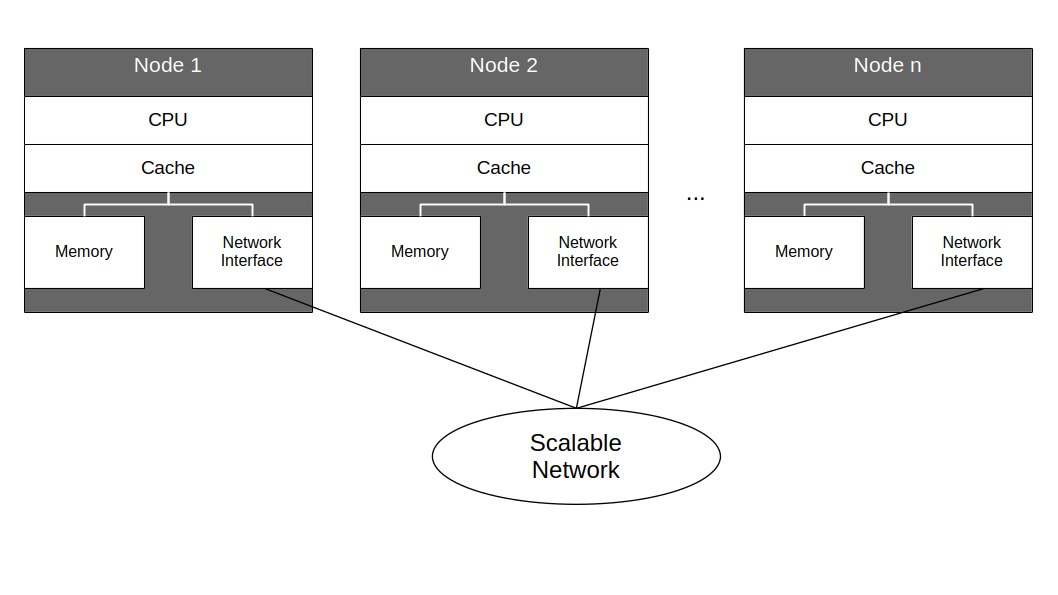
\includegraphics{figures/Diagrams/Setting.png}}
    \caption{Overview of the Setting}
    \label{fig:setting}
\end{figure}

\section{Preliminaries}\label{sec:prelimn}
A graph $G = (V, E \subseteq V \times V)$, where $V := \{v_0, v_1,..., v_{n-1}\}$ are the vertices of $G$ and $E := \{e_1, e_2,...,e_{n-1}\}$ are the edges. The graph may contain only one vertex and zero edges. The number of vertices $|V|$ is often called the order of $G$. A node and a edge are incident, if the node is an endpoint of the edge. The degree of a node is the number of incident edges. If a edge connects two vertices, these vertices are \textit{adjacent} to each other, or also refered to as \textit{neighboring vertices}. A loop is an edge with equal endpoints. Multiple edges are edges with same pair of endpoints. A simple graph has no loops, nor multiple edges. A clique is a set of pairwise adjacent vertices. A path is a simple graph whose vertices can be ordered such that two vertices are adjacent, if and only if they are consecutive in the list. A graph is connected if each pair of vertices in the graph $G$ belongs to a path. A graph is classified as bipartite graph, if the set of graph edges is the union of two disjoint independent sets. If $G$ has a path from node $u$ to node $v$, then the distance from $u$ to v, $d_G(u,v)$ is the shortest length from a $u,v-$path. $\text{diam} (G) := max_{u,v\in V}d_G(u,v)$ is the diameter of a graph. \cite{GraphTheorySchindelhaauer2021} 

\section{Motivation}\label{sec:motivation}
The motivation for this thesis stems from the observed performance discrepancies between the Single-Proposal Deal-Agreement-Based algorithm proposed by Yefim Dinitz, Shlomi Dolev and Manish Kumar \cite{Dinitz2023DAB} and the Push-Pull Sum algorithm described in the paper by Saptadi Nugroho, Alexander Weinmann and Christian Schindelhauer \cite{nugroho2023PushPullSumDataAg} across different network topologies. The obervations were gathered in a the student project with the title "Comparative Analysis of Load Balancing Algorithms in General Graphs" \cite{Bayazitoglu}. Judging from the simulations conducted in the student project, the Push-Pull Sum algorithm seems to perform better in reducing the MSE per round for the complete graph and the star graph compared to the Deal-Agreement-Based algorithm performing better in reducing the MSE per round for the torus grid graph and the ring graph. The simulations were conducted for different network sizes. The network size also played an role in faster convergence.

To address this, the proposed research introduces a novel algorithm, the Adaptive Threshold Push-Pull Sum algorithm that leverages the strengths of both algorithms, creating a Trade-off to mitigate their individual weaknesses. The newly introduced algorithm uses the mechanic of adaptive thresholding, in order to prevent load transfers with low effect in error reduction, since load transfers are pricy operations. By adapting to the structural characteristics of the investigated networks, this new solution aims to achieve robust performance across a wide range of scenarios, bridging the gap between the Deal-Agreement-Based algorithm and the Push-Pull Sum algorithm.

\section{Related Work}\label{sec:relatedwork}
Nugroho et al. \cite{nugroho2023PushPullSumDataAg} proposed the Push-Pull Sum algorithm, which essentially is a composition of two algorithms: the Push-Sum algorithm proposed by David Kempe, Alin Dobra and Johannes Gehrke \cite{kempe2003gossipbasedComp} and the Pull-Sum algorithm. The Push and the Pull mechanics are directly adopted from the Push-Pull Sum algorithm. Nugroho et al. used the mean squared error as a metric to evaluate the performance of their algorithm. In this thesis, I will follow an similar approach. Nugroho et al. conducted their experiments in static general graphs. This research also uses a static graph.  
Dinitz et al. \cite{Dinitz2023DAB} suggested two versions of the Single-Proposal Deal-Agreement-Based algorithm and two versions of a multi-neighbor Load Balancing algorithm, a round robin approach and a self-stabilizing load balancing algorithm. However the only comparable algorithm with ours are the Single-Proposal Deal-Agreement-Based algorithms, from which there exist two variations. One for the contiunous setting and one for the discrete setting. The main difference between these two is that in the contiunous setting any load may be transfered over the edges and in the discrete setting all load transfers must contain integers. For multi-neighbor load balancing the nodes may transfer loads to several neighbors in one round. For the Push-Pull-Sum algorithm this is only the case for the the pull actions where one node responds to every calling node by sending loads back. The self-stabilizing and the round robin approach are asynchronous algorithms, while the Adaptive-Threshold Push-Pull Sum and the Push-Pull Sum algorithms are synchronous algorithm.

\section{Hypothesis}\label{sec:hypothesis}
The Adaptive Threshold Push-Pull Sum load-balancing algorithm, which integrates key features of the Deal-Agreement-Based algorithm and the Push-Pull Sum algorithm, will demonstrate performances that is intermediate between the two in terms of MSE reduction across six distinct network topologies. Specifically, it is expected to perform better than the Deal-Agreement-Based algorithm in high-degree networks and perform better than the Push-Pull Sum algoithm in low-degree networks, achieving a balance that improves overall adaptability and efficiency compared to the both.

This hypothesis will be tested through comparative analysis of the MSE for six distinct topologies (some with different network sizes), demonstrating the algorithm's robustness and scalability across network environments. Model fitting is applied as a analysis technique to see the trend of the data and to be able to make statements regarding the convergence rate. Slopes are computed for three different regions labeled as \textit{Start}, \textit{Middle} and \textit{End}, in order to get details of the performance in specific time frames.

\section{Contribution}\label{sec:contribution}
This study introduces a novel load balancing algorithm that combines the strengths of two established approaches randomized load balancing and deal agreement-based balancing while integrating an adaptive threshold mechanism to enhance performance by adapting to the current state of the network. The load balancing algorithm uses the push and pull mechanics for convergence to a balanced state.
    \chapter{Problem Overview}\label{chap:problemoverview}
The load balancing problem is defined on an undirected general graph, where each node can transfer loads to its neighboring nodes via edges to achieve a balanced network state. The problem setting and the approach to address the problem are elaborated on in this section.

\section{Setting}\label{sec:setting}
\textbf{Continuous and Discrete}: In the continuous setting, nodes can transfer any amount of load over the edges, while in the discrete setting, all load transfers must consist of integer values.

\textbf{Synchronous and Asynchronous}:  In the synchronous setting, the time for message delivery is constant (e.g., O(1)), whereas in the asynchronous setting, the message delivery time can be unpredictably large. However, it is possible to convert an asynchronous setting into a synchronous one by adjusting the time frame within which messages are expected to be delivered.

\textbf{Static or Dynamic}: Load balancing algorithms can operate in either static or dynamic graph settings. In a dynamic graph, connections between nodes may change arbitrarily between rounds. In contrast, the connections and the nodes remain the same for the static graph.

The peer-to-peer network is modeled as a static general graph, meaning the set of edges remains unchanged during the application of the load balancing algorithms. The objective of load balancing is achieved using local algorithms, where each node gathers information only from its direct neighbors. The setting is a continuous setting. Additionally, a synchronous message delivery assumption is made, with a constant delivery time, e.g., O(1). The experiments are conducted on six distinct network topologies, each comprising $2^{10}$ nodes.

\section{Approach}\label{sec:approach}
This research consists of three steps: the design of a load balancing algorithm, the simulation phase to test its ability to balance the state of the network across different topologies, and a comparative analysis of the simulation outcomes using statistical methods. In prior research \cite{Bayazitoglu}, the strengths and weaknesses of two distinct load balancing algorithms were identified by simulating their performance on various topologies and network sizes to test the scalability and adaptability of the algorithms to different situations. The design of the novel adaptive threshold load balancing algorithm builds upon these findings. Each simulation outcome includes 30 distinct experiments to ensure statistical significance. The results are analyzed using the concept of model fitting to identify trends in MSE reduction, with slopes calculated for different regions to assess the consistency of performance. The findings are presented in plots, accompanied by explanations that provide insights into the observed behavior of the load balancing algorithms.

    \chapter{Algorithms}\label{chap:algorithms}
This thesis examines three load balancing algorithms: the Continuous Single-Proposal Deal-Agreement-Based algorithm, the Push-Pull Sum algorithm, and the newly proposed Adaptive Threshold Push-Pull Sum algorithm. The Adaptive Threshold Push-Pull Sums structure is described, along with how it incorporates features from the first two algorithms and the rationale behind its development. The working mechanics of each algorithm are described along with pseudo-code. Furthermore, examples are provided to show how the algorithms achieve a balanced state in the network. To provide further light on the objectives of the Adaptive Threshold Push-Pull Sum method, the aspired results are described.

\section{Characteristics}\label{sec:algoCharacteristics}
Like the graphs, load balancing algorithms may have different characteristics. These characteristics are elaborated on below:

\textbf{Static and Dynamic}: Load balancing algorithms can be classified as either static or dynamic algorithms. Static algorithms assign tasks to the nodes at compile time, while dynamic algorithms assign tasks at run time. The main advantage that static load balancing algorithms have over dynamic load balancing algorithms is that they do not cause any run-time overhead. \cite{Bokhari}

\textbf{Stochastic and Deterministic}: Stochastic load balancing algorithms rely on randomness to select load transfer partners. Deterministic load balancing algorithms, on the other hand, follow predefined distribution rules in order to make load transfers. \cite{ChengzhongFrancis}

\textbf{Global and Local}: Local load balancing algorithms allow nodes to transfer loads within their domain or neighborhood, while global load balancing algorithms enable load balancing operations across the entire network \cite{ChengzhongFrancis}.

\textbf{Monotonic and Non-monotonic}: An algorithm is considered monotonic if each load transfer is from a higher-loaded node to a less-loaded node and the maximal load in the network never increases and the minimal load never decreases \cite{Dinitz2023DAB}.

\textbf{Mass conservation property}: Some load balancing algorithms possess the mass conservation property, which guarantees that the values will converge to the correct aggregate of the network's ground truth \cite{nugroho2023PushPullSumDataAg}.

\textbf{Anytime}: An anytime algorithm can be halted at any stage during the execution, and after stoppage the state of the network is not worse than in any previous rounds. The advantage that comes with an anytime algorithm is that the network in which the load balancing algorithm with this property is applied is guaranteed to show more feasible states with intermediate rounds. \cite{Dinitz2023DAB}

Many of these properties are desirable for load balancing. For instance, monotonicity and the anytime property contribute to better performance and robustness, while locality reduces computational overhead. Similarly, determinism enhances the predictability and reliability of the algorithm's behavior.

\section{Push-Pull Sum Algorithm}\label{sec:classicPPS}
The Push-Pull Sum algorithm as proposed in \cite{nugroho2023PushPullSumDataAg} requires each node to hold sum $s_{i,r}$ and weight $w_{i,r}$ values as initial information. Initially, each node's weight is set to $w_{i,0} = 1$, and the sum of all weights is equal to the network size $N$ at each round. The sum of each node's initial sum values $s_{i,0}$ is equal to whatever the required input $x_i \in \mathbb{R}^{+}_{0}$ is, in the paper the values for the sums are uniformly distributed values between 0 and 100 \cite{nugroho2023PushPullSumDataAg}. The algorithm consists of three main procedures: \textit{RequestData}, \textit{ResponseData}, and \textit{Aggregate}, as detailed in algorithm \ref{alg:PPS}.

Each round $r$, except the first, begins with the \textit{Aggregate} procedure, where each node $i$ collects messages $M_{i,r}$ sent by other nodes $\{(s_m, w_m)\}$ in the previous round $r-1$, requesting data. Each node then updates its sum and weight values as $\sum_{m \in M_{i,r}}{s_m}$ and $\sum_{m \in M_{i,r}}{w_m}$, respectively. The updated load is computed by dividing the sum by the weight. Next, each node calls the \textit{RequestData} procedure. In this procedure, each node chooses a random neighbor node and executes a push operation, so each node sends half of its sum $\frac{s_{i,r}}{2}$ and half of its weight $\frac{w_{i,r}}{2}$ to the chosen neighbor and itself. Finally, each node executes the pull operation, which is described in the \textit{ResponseData} procedure. Here, each node gathers the incoming requests per round $r$ in a set $R_{i, r}$. Then, each node replies to each requesting node, including itself, by distributing half of its sum divided by the number of incoming requests $\frac{\frac{s_{i,r}}{2}}{|R_{i, r}|}$ to each requesting node.

\renewcommand{\algorithmicrequire}{\textbf{Input:}}
\renewcommand{\algorithmicensure}{\textbf{Output:}}
\begin{algorithm}[]
\caption{Push-Pull Sum algorithm}\label{alg:PPS}
\begin{algorithmic}[1]
\Procedure{RequestData}{}
\State Chose a random neighbor node $v$
\State Send $(\frac{s_{u,r}}{2}, \frac{w_{u,r}}{2})$ to the chosen node $v$ and the node $u$ itself
\EndProcedure
\Procedure{ResponseData}{}
\State $R_{u,r} \leftarrow$ Set of the nodes calling $u$ at a round $r$
\For{\textbf{all} $i \in R_{u,r}$}
\State Reply to i with $\left( \frac{\frac{s_{u,r}}{2}}{|R_{u,r}|}, \frac{\frac{w_{u,r}}{2}}{|R_{u,r}|} \right)$
\EndFor
\EndProcedure
\Procedure{Aggregate}{}
\State $M_{u,r} \leftarrow \{(s_{m}, w_{m})\}$ messages sent to $u$ at a round $r-1$
\State $s_{u,r} \leftarrow \sum_{m \in M_{u,r}}^{}s_{m}, w_{u,r} \leftarrow\sum_{m \in M_{u,r}}^{}w_{m}$
\State $f_{avg} \leftarrow \frac{s_{u,r}}{w_{u,r}}$
\EndProcedure
\end{algorithmic}
\end{algorithm}


The setting in \cite{nugroho2023PushPullSumDataAg} is similar to ours. While their study focuses on a Complete graph with $10^{4}$ nodes, this study examines network sizes of $2^{10}$ nodes and includes different topologies. In that paper, 50 experiments were conducted, each running for 30 rounds. Their findings demonstrated that the Push-Pull Sum algorithm reduces the expected potential $\Phi_r$ exponentially. The potential function for the Complete graph is defined as:
\begin{align}
    \Phi_r=\sum_{i,j}\left(v_{i,j,r}-\frac{w_{i,r}}{n}\right)^{2},  
\end{align} where the $v_{i,j,r}$ component stores the fractional value of node $j$'s contribution at round $r$. The equation: 
\begin{align}
    \mathbb{E}[\Phi_{r+1}|\Phi_r=\phi]=(\frac{2e-1}{4e}-\frac{1}{4n})\phi    
\end{align}
is the conditional expectation of $\Phi_r+1$ for the Push-Pull Sum algorithm. The Push-Pull Sum algorithm holds the mass-conservation property and is classified as a stochastic load balancing algorithm due to its randomized neighbor selection process \cite{nugroho2023PushPullSumDataAg}.

The Push-Pull Sum algorithm performed very well on Complete graphs, Ring of Cliques with large clique size, Lollipop graphs with large clique size, and Star graphs. In the case of the Star graph the internal node acts as a distributor of the load. Since each leaf chooses the internal node with 100\% possibility as a "random" neighbor the internal node is involved as a endpoint of $N-1$ external push operations, and redistributes the load via pull operations to the leaves, where the sum is $\frac{\frac{s_{i,r}}{2}}{N-1}$ and accordingly the weight is $\frac{\frac{w_{i,r}}{2}}{N-1}$. For for the Complete graph, the Ring of Cliques and the Lollipop graph, the density of the graph plays an crucial role. Since nodes select neighbors randomly, the high edge density allows the algorithm to spread loads efficiently and prevent bottlenecks. This explains why the Push-Pull Sum algorithm underperformed on Torus Grid and Ring graphs compared to the Single-Proposal Deal-Agreement-Based algorithm, as they are limited to a degree of four and two respectively.

\subsection{Example}\label{subsec:examplePPS}
\begin{figure}
    \centering
    \scalebox{0.75}{\begin{tikzpicture}[scale=0.75, thick, main node/.style={circle, draw, minimum size=1.2cm}]

    % First graph
    \node[main node] (A1) at (-1,4.5) {A};
    \node[main node] (B1) at (3,4.5) {B};
    \node[main node] (C1) at (-1,0) {C};
    \node[main node] (D1) at (3,0) {D};
    
    \node[above, color=blue] at (A1.north) {(3, 1)};
    \node[above, color=blue] at (B1.north) {(15, 1)};
    \node[below, color=blue] at (C1.south) {(62, 1)};
    \node[below, color=blue] at (D1.south) {(44, 1)};

    \node[above, color=blue] at (-1,6) {$R_{A,1}=\{\}$};
    \node[above, color=blue] at (3,6) {$R_{B,1}=\{\}$};
    \node[above, color=blue] at (-1,-2.2) {$R_{C,1}=\{\}$};
    \node[above, color=blue] at (3,-2.2) {$R_{D,1}=\{\}$};

     \node[above, color=blue] at (7.5,6) {$R_{A,1}=\{A, B\}$};
    \node[above, color=blue] at (11.5,6) {$R_{B,1}=\{B, C, D\}$};
    \node[above, color=blue] at (7.5,-2.2) {$R_{C,1}=\{A, C\}$};
    \node[above, color=blue] at (11.5,-2.2) {$R_{D,1}=\{\}$};
    
    \draw (A1) -- (B1);
    \draw (A1) -- (C1);
    \draw (A1) -- (D1);
    \draw (B1) -- (C1);
    \draw (B1) -- (D1);
    \draw (C1) -- (D1);

    % Second graph
    \node[main node] (A2) at (7.5,4.5) {A};
    \node[main node] (B2) at (11.5,4.5) {B};
    \node[main node] (C2) at (7.5,0) {C};
    \node[main node] (D2) at (11.5,0) {D};
    
    \node[above, color=blue] at (A2.north) {$(9, 1)$};
    \node[above, color=blue] at (B2.north) {$(60.5, 1.5)$};
    \node[below, color=blue] at (C2.south) {$(32.5, 1)$};
    \node[below, color=blue] at (D2.south) {$(22, 0.5)$};
    
    \draw (A2) -- (B2);
    \draw (A2) -- (C2);
    \draw (A2) -- (D2);
    \draw (B2) -- (C2);
    \draw (B2) -- (D2);
    \draw (C2) -- (D2);

    \draw[->] (A1) to[out=240, in=120] node[left, scale=0.8] {$(1.5, 0.5)$} (C1);
    \draw[->] (B1) to[out=150, in=30] node[above, scale=0.8] {$(7.5, 0.5)$} (A1);
    \draw[->] (C1) to[out=30, in=240] node[right, scale=0.8] {$(31, 0.5)$} (B1);
    \draw[->] (D1) to[out=60, in=300] node[right,scale=0.8] {$(22, 0.5)$} (B1);


    
    %\draw[dashed, ->] (C1) to[out=60, in=300] node[right] {$\frac{l_{C}-l_{A}}{2}$} (A1);
    %\draw[dashed, ->] (A1) to[out=330, in=210] node[right] {$\frac{l_{C}-l_{A}}{2}$} (B1);
    

    
    \draw[dashed, ->] (C2) to[out=60, in=300] node[left, scale=0.8 ] {$(15.5, 0.25)$} (A2);
    \draw[dashed, ->] (A2) to[out=-30, in=210] node[above, scale=0.8] {$(0.75, 0.25)$} (B2);
    \draw[dashed, ->] (B2) to[out=240, in=30] node[right, scale=0.8] {$(2.5,0.167)$} (C2);
    \draw[dashed, ->] (B2) to[out=300, in=60] node[right, scale=0.8] {$(2.5,0.167)$} (D2);

    % Legend in the middle below the graphs
    \begin{scope}[shift={(3,-3)}]
        % Horizontal line
        \draw (-4,0) -- (-3,0) node[right] {connecting edge};
        % Long right arrow
        \draw[->, line width=1pt] (-4,-1) -- (-3,-1) node[right] {Push};
        % Long right dashed arrow
        \draw[->, dashed, line width=1pt] (-4,-2) -- (-3,-2) node[right] {Pull};
        
        % Load notation
        \node at (5,0) {$(s_{i,r}, w_{i,r})$ : sum and weight values};
        \node at (5.3,-1) {$R_{i,r}$ : Set of nodes calling i at round r};
    \end{scope}

\end{tikzpicture}}
    \caption{Push-Pull Sum: push and pull actions}
    \label{fig:examplePPSSetting}
\end{figure}

The example in figure \ref{fig:examplePPSSetting} illustrates a execution of the Push-Pull Sum algorithm on a Complete graph $K_4$ with four nodes labeled \textit{A, B, C} and \textit{D}. Each node is initially assigned a sum and a weight value. The undirected graph represents the network topology, showing connections between neighboring nodes. The solid directed edges depict the push operations and the dashed directed edges visualize the pull operations. Each node maintains a set $R_{i,r}$ where $i$ is the node ID and $r$ is the round being examined. The load of the node is calculated by $\frac{s_{i,r}}{w_{i,r}}$. The example depicts the first round of a execution of the Push-Pull Sum algorithm. The push and pull operations are distinct. The left-hand side of figure \ref{fig:examplePPSSetting} depicts the behavior of the nodes while executing the push operations, while the right side illustrates the pull operations. During the push phase, each node randomly selects a neighbor to transfer load to. In this example:

\begin{itemize}
    \item Node $A$ selects node $C$ and pushes half of its sum and weight to both node $C$ and itself. (Self-loops are omitted from the figure for readability.)
    \item Node $B$ selects node $A$ as its trading partner.
    \item Nodes $C$ and $D$ push their values to node $B$ and themselves.
\end{itemize}

Given the push operations for each node, the set $R_{i,r}$ is computed. Since node $B$ pushed load to node $A$ and node $A$ pushed load to itself, we get $R_{A,1}=\{A,B\}$. The updated sum and weight values after the push phase can be inspected on the right-hand side of figure \ref{fig:examplePPSSetting}.

Following the push actions, each node proceeds with the \textit{ResponseData}-procedure, executing the pull phase. Each node in $R_{i,1}$ receives a response based on the respective pull values. Since node $A$ has two nodes in its set $R_{A,1}$, it responds to both node $B$ and itself with $\left(\frac{\frac{3}{2}}{2}, \frac{\frac{1}{2}}{2}\right)$, as indicated by a dashed directed edge. Similarly, the remaining nodes \textit{B, C, and D} execute their pull operations. Following the push and pull operations, the nodes update their sum and weight values. The state of the network after round one is depicted in figure \ref{fig:examplePPSResult}. The MSE at the beginning of round 1 is $542.50$. After applying one round of the Push-Pull Sum algorithm, the MSE is reduced to $63.49$.

\begin{figure}
    \centering
    \scalebox{0.75}{\begin{tikzpicture}[scale=0.75, thick, main node/.style={circle, draw, minimum size=1.2cm}]

    % First graph
    \node[main node] (A1) at (-1,4.5) {A};
    \node[main node] (B1) at (3,4.5) {B};
    \node[main node] (C1) at (-1,0) {C};
    \node[main node] (D1) at (3,0) {D};
    
    \node[above, color=blue] at (A1.north) {$(23.75,1)$};
    \node[above, color=blue] at (B1.north) {$(56.25, 1.416)$};
    \node[below, color=blue] at (C1.south) {$(19.5, 0.9167)$};
    \node[below, color=blue] at (D1.south) {$(24.5, 0.67)$};
    
    \draw (A1) -- (B1);
    \draw (A1) -- (C1);
    \draw (A1) -- (D1);
    \draw (B1) -- (C1);
    \draw (B1) -- (D1);
    \draw (C1) -- (D1);

\end{tikzpicture}}
    \caption{Push-Pull Sum: setting after round 1}
    \label{fig:examplePPSResult}
\end{figure}

\section{Continuous Single-Proposal Deal-Agreement-Based Algorithm}\label{sec:singleproposalDAB}
The Continuous Single-Proposal Deal-Agreement-Based algorithm proposed by Dinitz et al. \cite{Dinitz2023DAB} is unlike the Push-Pull Sum algorithm, not a diffusion-based algorithm. The goal of load balancing is achieved based on deterministic deal agreements, where one node proposes a load to one neighboring node, and the neighboring node either accepts the transfer proposal either fully or partially. Dinitz et al. proved that the algorithm has the anytime property, meaning it never worsens the state of the network during execution. Their study examined the algorithm in a dynamic setting, where each node has access to a set of neighboring nodes, including the node's loads. The algorithm is divided into three phases: \textit{proposal}, \textit{deal}, and \textit{summary}. In the \textit{proposal}-phase, each node $u$ identifies its minimally loaded neighbor \textit{v} and sends a proposal to that neighbor if $v$ has a lower load. The proposal is of value:
\begin{align}
    \frac{load_{r}(u)-load_{r}(v)}{2}    
\end{align}
which is labeled as a \textit{fair} proposal. Since the load transfer is fair, the resulting load of $u$ is not lower than that of $v$. $load_{r}(u)$ represents the load of node $u$ at round $r$. In the \textit{deal}-phase, nodes evaluate the deals proposed to them. A node accepts the deal of the node that proposes the maximal load transfer. The actual transfer happens, and the nodes update their loads. Finally, in the \textit{summary}-phase, each node informs their neighbors regarding their updated load values. \cite{Dinitz2023DAB}

\renewcommand{\algorithmicrequire}{\textbf{Input:}}
\renewcommand{\algorithmicensure}{\textbf{Output:}}
\begin{algorithm}
\caption{Continuous Single-Proposal Deal-Agreement-Based protocol}\label{alg:DAB}
\begin{algorithmic}[1]
\Require An undirected graph $G=(V,E,load)$
\Ensure A load state with discrepancy at most $\epsilon$ on $G$
\For{$r=1$ and on}
\For{every node u}
\State Find a neighbor, $v$, with the minimal load
\If{$load_{r}(u) - load_{r}(v)>0$}
\State $u$ sends to $v$ a transfer proposal of value $(load_{r}(u)-load_{r}(v))/2$
\EndIf
\EndFor

\For{every node $u$}
\If{there is at least one transfer proposal to $u$}
\State Find a neighbor, $w$, proposing to $u$ the maximal transfer
\State Node $u$ makes a deal: informs node $w$ on accepting its proposal
\State The actual transfer from $w$ to $u$ is executed 
\EndIf
\EndFor

\For{every node $u$}
\State Node $u$ sends the updated value of its load to its neighbors
\EndFor
\EndFor
\end{algorithmic}
\end{algorithm}


The analysis in Dinitz et al.\cite{Dinitz2023DAB} is based on a potential function that measures the network. The potential for a node $u$ is defined as:
\begin{align}
    p(u) = (load(u)-L_{avg})^{2}    
\end{align}
where $L_{avg}$ represents the current load average in the network. The potential for the graph $p(G)$ is defined as:
\begin{align}
    p(G)=\sum_{u\in V}{p(u)},   
\end{align}
which is the sum of all potential of each node in the graph G. Any fair load transfer of load $l$ decreases the potential of the graph by at least $2*l^{2}$. As a result of any round $r$ of the Continuous Single-Proposal Deal-Agreement-Based algorithm, the graph potential decreases by at least $\frac{K^{2}_r}{2D_r}$, where $K$ is the initial discrepancy and $D$ is a bound for the graph diameter. \cite{Dinitz2023DAB}

The Single-Proposal Deal-Agreement-Based load balancing algorithm struggles to reduce the MSE as rapidly as the Push-Pull Sum algorithm for dense graphs like the Complete graph, the Lollipop graph with a large clique size, and the Ring of Cliques with a large clique size. This limitation arises because each node seeks the minimally loaded partner for load transfer. For a Complete graph, the minimal load partner is the same node with loads of $L_{min}$ (the minimally loaded node in the network). This causes each node to propose to the same node, which then evaluates the proposals and accepts exactly one transfer proposal, namely the maximal one. This situation is described in detail in the appendix in section \ref{sec:struggleDAB} using an example. A similar scenario occurs in the Ring of Cliques and the Lollipop graph. However, in the Ring of Cliques, nodes do not all propose to the same minimal neighbor, instead, they propose to the least-loaded neighbor within their respective cliques. For the Lollipop graph, the nodes in the path graph balance their loads more quickly than the nodes in the clique, which is a bottleneck in this scenario. For the Torus Grid and the Ring graph, the Deal-Agreement-Based algorithm performs better in reducing the error. In these scenarios, the proposals are more evenly distributed among nodes due to the lower density of the graphs. The Star graph is an exception to this case, since we have a similar bottleneck as in the Complete graph, since the internal node is the common neighbor for each leaf, and thus each leaf proposes a load to the internal node. The internal node can accept only one proposal. Again, an example to this is provided in the appendix in section \ref{sec:struggleDAB}.

\subsection{Example}\label{subsec:exampleDAB}
 \begin{figure}
    \centering
    \scalebox{0.75}{\begin{tikzpicture}[ thick, main node/.style={circle, draw, minimum size=1.2cm}]

    % First graph
    \node[main node] (A1) at (0.5,4.5) {A};
    \node[main node] (B1) at (4.5,4.5) {B};
    \node[main node] (C1) at (0.5,0) {C};
    \node[main node] (D1) at (4.5,0) {D};
    
    \node[above, color=blue] at (A1.north) {3};
    \node[above, color=blue] at (B1.north) {15};
    \node[below, color=blue] at (C1.south) {62};
    \node[below, color=blue] at (D1.south) {44};
    
    \draw (A1) -- (B1);
    \draw (A1) -- (C1);
    \draw (A1) -- (D1);
    \draw (B1) -- (C1);
    \draw (B1) -- (D1);
    \draw (C1) -- (D1);

    % Second graph
    \node[main node] (A2) at (7.5,4.5) {A};
    \node[main node] (B2) at (11.5,4.5) {B};
    \node[main node] (C2) at (7.5,0) {C};
    \node[main node] (D2) at (11.5,0) {D};
    
    \node[above, color=blue] at (A2.north) {32.5};
    \node[above, color=blue] at (B2.north) {15};
    \node[below, color=blue] at (C2.south) {32.5};
    \node[below, color=blue] at (D2.south) {44};
    
    \draw (A2) -- (B2);
    \draw (A2) -- (C2);
    \draw (A2) -- (D2);
    \draw (B2) -- (C2);
    \draw (B2) -- (D2);
    \draw (C2) -- (D2);

    \draw[->] (C1) to[out=120, in=240] node[left] {$29.5$} (A1);
    \draw[dashed, ->] (C1) to[out=60, in=300] node[right] {$29.5$} (A1);
    \draw[dashed, ->] (B1) to[out=210, in=330] node[above] {$6$} (A1);
    \draw[dashed, ->] (D1) to[out=120, in=330] node[right] {$20.5$} (A1);

    % Legend in the middle below the graphs
    \begin{scope}[shift={(3,-2)}]
        % Horizontal line
        \draw (-2,0) -- (-1,0) node[right] {connecting edge};
        % Long right arrow
        \draw[->, line width=1pt] (-2,-1) -- (-1,-1) node[right] {actual deal};
        % Long right dashed arrow
        \draw[->, dashed, line width=1pt] (-2,-2) -- (-1,-2) node[right] {proposal};
        
        % Load notation
        \node at (4,0) {$l_{node}$ : load of node};
        \node at (5,-1) {$t_{x,y}$ : transfered load from x to y};
    \end{scope}

\end{tikzpicture}}
    \caption{Deal-Agreement-Based: initial setup and setup after round 1}
    \label{fig:DABExampleAlgo}
 \end{figure}
Figure \ref{fig:DABExampleAlgo} illustrates two settings. The left-hand side of the figure depicts the initial state and the right-handside illustrates the state after one round of execution. The setting is the same as in the example above for the Push-Pull Sum, with the difference that each node is assigned a load value, instead of sum and weight values. In the figure, dashed directed edges represent transfer proposals from one node to another, while solid directed edges indicate actual load transfers. The network consists of four nodes, labeled \textit{A, B, C,} and \textit{D}. Each node identifies its least-loaded neighbor as a potential transfer recipient. Nodes \textit{B, C} and \textit{D} determine node $A$ as their minimal loaded neighbors. Node $A$ identifies node $B$ as the neighbor with the minimal load in its neighborhood, however node $B$ has more load than node $A$, so node $A$ does not send an transfer proposal to node $B$. As a result, nodes \textit{B, C} and \textit{D} each send a transfer proposal of value $\frac{(load_r(i)-load_r(A))}{2}$ to node $A$, where $i \in \{B,C,D\}$. Node $A$ evaluates the proposal and accepts node $C$'s transfer proposal, as node $C$ proposes the largest amount of load, namely $29.5$. The actual transfer happens and $29.5$ of loads are transfered from node $C$ to node $A$. The right-hand side of figure \ref{fig:DABExampleAlgo} shows the state of the network after round 1 of executing the Deal-Agreement-Based algorithm. Node $A$ and $C$ each have equal loads of $32.5$, the loads of nodes $B$ and $D$ remain unchanged. The MSE at the beginning of round 1 is at $542.5$. After executing the first round of the algorithm the MSE decreases to a value of $107.375$, which is approximately one-fifth of the initial MSE.

\section{Adaptive Threshold Push-Pull Sum Algorithm}\label{sec:adaptivethresholdPPS}
The Adaptive Threshold Push-Pull Sum algorithm is composed of key elements from both the Push-Pull Sum and Single-Proposal Deal-Agreement-Based algorithms, extended by the idea of adaptive thresholding. The Adaptive Threshold Push-Pull Sum consists of different procedures. In the \textit{CheckThresholdsRequestData}, each node $u$ chooses a subset $RN_{u,r}$ with:
\begin{align}
    RN_{u,r} \subseteq neighborhood_{u}, |RN_{u,r}|=\lceil \log_{2}{(|neighborhood_{u}|)} \rceil
\end{align}
random neighbors. This increases the likelihood of selecting a well-suited neighbor for load transfer. Selecting only one random neighbor lowers the chance to find an optimal or good neighbor to execute a load transfer. Then the load difference between the node $u$ and each node in $RN_{u,r}$ is computed and checked against a threshold $\theta$. The threshold is computed in the \textit{CalculateThresholds}-procedure. The threshold $\theta$ is calculated as:
\begin{align}
    \theta = k*\sqrt{MSE_r-1}    
\end{align}
where $k$ is some factor to adjust the sensitivity of the threshold. A larger $k$ makes the threshold more sensitive, meaning that fewer nodes are eligible for load transfer, allowing only significant load transfer. Respectively, a smaller $k$ makes the threshold less strict; thus, more nodes are eligible for load transfers. This condition ensures that only load transfers with meaningful impact happen, and load transfers between nodes with low impact on the balance of the network are avoided. The first eligible node in $RN_{u,r}$ that exceeds the threshold receives the sum of value $(\frac{s_i,r}{2})$ and the weight of value $(\frac{w_i,r}{2})$. The \textit{ResponseData} and the \textit{Aggregate}-procedure are directly adapted from the Push-Pull Sum algorithm. The way the loads are distributed, is directly taken from the Push-Pull Sum algorithm and extended by an adaptive threshold mechanism. Like the Single-Proposal Deal-Agreement-Based algorithm, the Adaptive Threshold Push-Pull Sum algorithm employs conditional load transfers, but with a threshold $\theta$ instead of requiring a strictly positive load difference. Instead of initiating a load transfer with the maximally proposing node, the Adaptive Threshold Push-Pull Sum algorithm orders the nodes to initiate a load transfer with the first node proposing load. The reason for that is to reduce computational overhead by avoiding that each node looks through its whole set $RN$ and is required to evaluate each proposal. So the first node proposing a load transfer is accepted as a transfer partner.

Although formally not shown, the Adaptive Threshold Push-Pull Sum algorithm is expected to hold the mass conservation property, as it converged to the correct ground truth in all experiment settings, similar to the Push-Pull Sum algorithm. Also, given that the push and pull mechanisms are directly adapted, these operations are the only operations that let nodes transfer or receive nodes in the algorithm. The Adaptive Threhsold Push-Pull Sum algorithm inherits is an stochastic algorithm as it inherits its stochastic nature from the Push-Pull Sum algorithm, by choosing a subset of neighbors randomly.

\begin{algorithm}
    \caption{Adaptive Threshold Push-Pull Sum algorithm}\label{alg:PPS}
    \begin{algorithmic}[1]
    \Procedure{CalculateThresholds}{}
    \State $\theta \leftarrow k * \sqrt{MSE_{r-1}}$ 
    \EndProcedure
    \Procedure{CheckTresholdRequestData}{}
    \State $RN_{u,r} \leftarrow$ choose $\lceil \log_{2}{(|neighborhood(u)|)} \rceil$ random neighbor
    \For{every node $v_{i} \in RN_{u,r}$}
    \State $\Delta_{u, v_{i}} \leftarrow |(load(u) - load(v_{i}))|$
    \If{$\Delta_{u,v} > \theta$}
    \State Send $(\frac{s_{u,r}}{2}, \frac{w_{u,r}}{2})$ to first node v fulfilling condition and the node $u$ itself
    \EndIf
    \EndFor
    \EndProcedure
    \Procedure{ResponseData}{}
    \State $R_{u,r} \leftarrow$ Set of the nodes calling $u$ at a round $r$
    \For{\textbf{all} $i \in R_{u,r}$}
    \State Reply to i with $\left( \frac{\frac{s_{u,r}}{2}}{|R_{u,r}|}, \frac{\frac{w_{u,r}}{2}}{|R_{u,r}|} \right)$
    \EndFor
    \EndProcedure
    \Procedure{Aggregate}{}
    \State $M_{u,t} \leftarrow \{(s_{m}, w_{m})\}$ messages sent to $u$ at a round $r-1$
    \State $s_{u,t} \leftarrow \sum_{m \in M_{u,r}}^{}s_{m}, w_{u,r} \leftarrow\sum_{m \in M_{u,r}}^{}w_{m}$
    \State $load(u) \leftarrow \frac{s_{u,r}}{w_{u,r}}$
    \EndProcedure
    \end{algorithmic}
    \end{algorithm}

\subsection{Example}\label{subsec:exampleAdaptiveThresholdPPS}
\begin{figure}
    \centering
    \scalebox{0.75}{\begin{tikzpicture}[scale=0.75, thick, main node/.style={circle, draw, minimum size=1.2cm}]

    % First graph
    \node[main node] (A1) at (-1,4.5) {A};
    \node[main node] (B1) at (3,4.5) {B};
    \node[main node] (C1) at (-1,0) {C};
    \node[main node] (D1) at (3,0) {D};
    
    \node[above, color=blue] at (A1.north) {(3, 1)};
    \node[above, color=blue] at (B1.north) {(15, 1)};
    \node[below, color=blue] at (C1.south) {(62, 1)};
    \node[below, color=blue] at (D1.south) {(44, 1)};

    \node[above, color=blue] at (-1,6) {$RN_{A,1}=\{B,C\}$};
    \node[above, color=blue] at (3,6) {$RN_{B,1}=\{A,C\}$};
    \node[above, color=blue] at (-1,-2.2) {$RN_{C,1}=\{A,B\}$};
    \node[above, color=blue] at (3,-2.2) {$RN_{D,1}=\{A,B\}$};

     \node[above, color=blue] at (7.5,6) {$R_{A,1}=\{A, B, C, D\}$};
    \node[above, color=blue] at (11.5,6) {$R_{B,1}=\{A, B\}$};
    \node[above, color=blue] at (7.5,-2.2) {$R_{C,1}=\{\}$};
    \node[above, color=blue] at (11.5,-2.2) {$R_{D,1}=\{\}$};
    
    \draw (A1) -- (B1);
    \draw (A1) -- (C1);
    \draw (A1) -- (D1);
    \draw (B1) -- (C1);
    \draw (B1) -- (D1);
    \draw (C1) -- (D1);

    % Second graph
    \node[main node] (A2) at (7.5,4.5) {A};
    \node[main node] (B2) at (11.5,4.5) {B};
    \node[main node] (C2) at (7.5,0) {C};
    \node[main node] (D2) at (11.5,0) {D};
    
    \node[above, color=blue] at (A2.north) {$(62, 2)$};
    \node[above, color=blue] at (B2.north) {$(9, 1)$};
    \node[below, color=blue] at (C2.south) {$(31, 0.5)$};
    \node[below, color=blue] at (D2.south) {$(22, 0.5)$};
    
    \draw (A2) -- (B2);
    \draw (A2) -- (C2);
    \draw (A2) -- (D2);
    \draw (B2) -- (C2);
    \draw (B2) -- (D2);
    \draw (C2) -- (D2);

    \draw[->] (A1) to[out=30, in=150] node[above, scale=0.8] {$(1.5, 0.5)$} (B1);
    \draw[->] (B1) to[out=210, in=-30] node[above, scale=0.8] {$(7.5, 0.5)$} (A1);
    \draw[->] (C1) to[out=120, in=240] node[right, scale=0.8] {$(31, 0.5)$} (A1);
    \draw[->] (D1) to[out=120, in=-30] node[right, scale=0.8] {$(22, 0.5)$} (A1);


    
    %\draw[dashed, ->] (C1) to[out=60, in=300] node[right] {$\frac{l_{C}-l_{A}}{2}$} (A1);
    %\draw[dashed, ->] (A1) to[out=330, in=210] node[right] {$\frac{l_{C}-l_{A}}{2}$} (B1);
    

    
    \draw[dashed, ->] (A2) to[out=30, in=150] node[below, scale=0.8] {$(0.375, 0.125)$} (B2);
     \draw[dashed, ->] (A2) to[out=240, in=120] node[left, scale=0.8] {$(0.375, 0.125)$} (C2);
     \draw[dashed, ->] (A2) to[out=-30, in=120] node[right, scale=0.8] {$(0.375,0.125)$} (D2);
      \draw[dashed, ->] (B2) to[out=210, in=-30] node[above, scale=0.8] {$(3.75,0.25)$} (A2);

    % Legend in the middle below the graphs
    \begin{scope}[shift={(3,-3)}]
        % Horizontal line
        \draw (-4,0) -- (-3,0) node[right] {connecting edge};
        % Long right arrow
        \draw[->, line width=1pt] (-4,-1) -- (-3,-1) node[right] {Push};
        % Long right dashed arrow
        \draw[->, dashed, line width=1pt] (-4,-2) -- (-3,-2) node[right] {Pull};
        
        % Load notation
        \node at (5,0) {$(s_{i,r}, w_{i,r})$ : sum and weight values};
        \node at (5,-1) {$RN_{i,r}$ : possible random neighbors};
        \node at (5.3,-2) {$R_{i,r}$ : Set of nodes calling i at round r};
    \end{scope}

\end{tikzpicture}}
    \caption{Adaptive Threshold Push-Pull Sum: push and pull actions}
    \label{fig:ATPPSExampleSetting}
\end{figure}

Figure \ref{fig:ATPPSExampleSetting} depicts a similar setting as described in section \ref{subsec:examplePPS}. According to the Adaptive Threshold Push-Pull Sum algorithm, each node chooses $\lceil \log_{2}{(|neighborhood|)} \rceil$ neighbors. For this setting, each node chooses two neighbors, which are added to the set $RN_{i,1}$ for each node $i$. For instance, node $A$ computes $RN_{A,1}$ as $\{B,C\}$. The load differences between node $A$ and nodes $B$ and $C$ are computed. In this example, $k$ is set to $0.01$, thus the threshold $\theta$ is given by $0.01*\sqrt{542.5} \approx 0.23$. Since both load differences between nodes $A$ and $B$ and nodes $A$ and $C$ exceed this threshold, both nodes are eligible to propose a load transfer with node $A$. In this scenario, node $A$ selects node $B$ as a transfer partner and pushes half of its sum $1.5$ and weight $0.5$ to node $B$ and itself. This process is repeated for each node accordingly. Similar to the example in section \ref{subsec:examplePPS}, the nodes then execute the pull operation. The result is depicted in figure \ref{fig:ATPPSExampleResult}. The MSE dropped from $542.5$ initially to $251.86$. The error reduction depends on the sensitivity factor $k$. If $k$ is set to 1, the load transfer between node $A$ and $B$ would not have happened. Instead, nodes $A$ and $C$ would have exchanged loads, leading to a larger impact on the balance of the network. 

\begin{figure}
    \centering
    \scalebox{0.75}{\begin{tikzpicture}[scale=0.75, thick, main node/.style={circle, draw, minimum size=1.2cm}]

    % First graph
    \node[main node] (A1) at (-1,4.5) {A};
    \node[main node] (B1) at (3,4.5) {B};
    \node[main node] (C1) at (-1,0) {C};
    \node[main node] (D1) at (3,0) {D};
    
    \node[above, color=blue] at (A1.north) {$(64.625,1.875)$};
    \node[above, color=blue] at (B1.north) {$(5.625, 0.875)$};
    \node[below, color=blue] at (C1.south) {$(31.375, 0.625)$};
    \node[below, color=blue] at (D1.south) {$(22.375, 0.625)$};
    
    \draw (A1) -- (B1);
    \draw (A1) -- (C1);
    \draw (A1) -- (D1);
    \draw (B1) -- (C1);
    \draw (B1) -- (D1);
    \draw (C1) -- (D1);

    \node at (1,6.5) {network after round 1};


\end{tikzpicture}}
    \caption{Adaptive Threshold Push-Pull Sum: setting after round 1}
    \label{fig:ATPPSExampleResult}
\end{figure}
\subsection{Aspired Outcome}\label{subsec:aspiredOutcomeAdaptiveThresholdPPS}

Considering the simulation results presented in \cite{Bayazitoglu}, the discrepancy between the MSE reduction abilities per round for the different topologies shows that the algorithms perform either very well or mediocre to bad. The primary motivation behind designing the Adaptive Threshold Push-Pull Sum algorithm was to find a compromise solution that enhances adaptability across various network topologies.

The final results of the first load balancing step can be taken from table \ref{tab:overviewExamples}. The Push-Pull Sum algorithm shows the lowest MSE after round one, followed by the Deal-Agreement-Based algorithm and the Adaptive Threshold Push-Pull Sum algorithm. A small $k$ value was used for demonstrative purposes (as the simulations were conducted with small $k$ values). A higher k value would have a greater impact in the first round. In section \ref{chap:simulationoutcomes}, we will see that the Adaptive Threshold Push-Pull Sum algorithm proceeds to enhance in reducing error in later rounds, as the MSE and thus the thresholds adjust.

\begin{table}
\centering
\begin{tabular}{|c|c|c|c|c|}
\hline
 & \textbf{Initial} & \textbf{Dinitz et al.} & \textbf{Nugroho et al.} & \textbf{Bayazitoglu} \\ \hline
\textbf{Node A}  & 3      & 32.5    & (23.75, 1) = 23.75     & (64.625, 1.875) = 34.47 \\ \hline
\textbf{Node B}  & 15     & 15      & (56.25, 1.416) = 39.72 & (5.625, 0.875) = 6.43   \\ \hline
\textbf{Node C}  & 62     & 32.5    & (19.5, 0.9167) = 21.27 & (31.375, 0.625) = 50.2  \\ \hline
\textbf{Node D}  & 44     & 44      & (24.5, 0.67) = 36.57   & (22.375, 0.625) = 35.8  \\ \hline
\textbf{MSE} & 542.50 & 107.375 & 63.49                  & 251.86                  \\ \hline
\end{tabular}
\caption{Overview over example outcomes}
\label{tab:overviewExamples}
\end{table}
    \chapter{Topologies}\label{chap:topologies}
The simulations were conducted for six distinct network topologies. Each network has $2^{10}$ (1024) nodes. The behavior of the algorithms in these different topologies is observed, since each topology has different characteristics; different performances exploiting the specials of the topologies are expected. The topologies contain \textit{Complete graph}, \textit{Torus Grid graph}, \textit{Ring graph}, \textit{Star graph}, \textit{Lollipop graph}, and \textit{Ring of Cliques}. In the following, the topologies including these characteristics are presented.

\section{Complete Graph}\label{sec:2completegraph}
The Complete graph $K_N$, as illustrated in \hyperref[fig:completegraphDemo]{figure} \ref{fig:completegraphDemo}, is a graph where each pair of distinct nodes is connected by an edge. The Complete graph, also referred to as a fully connected graph, has $N$ nodes and $\frac{N\times(N-1)}{2}$ edges. The Complete graph is a regular graph, where each node has a degree of $N-1$. As it contains the maximum possible number of edges for a given set of nodes, it is considered a dense graph \cite{GraphTheorySchindelhaauer2021}. The diameter of a Complete graph is 1, as each node is directly connected to every other node. Since each node has the same degree and connectivity, algorithms can treat all nodes uniformly.

The Complete graph is used in financial trading systems and military communications, where high reliability and low latency are critical. The Complete graph ensures optimal routing paths between nodes, due to its low diameter \cite{Banerjee2001}.

\begin{figure}[H]
    \centering
    \begin{tikzpicture}
    \foreach \i in {1,...,16} {
      \node[draw, fill=blue, circle, minimum size=4pt] (v\i) at ({360/16 * (\i-1)}:3) {};
    }
    
    \foreach \i in {1,...,16} {
      \foreach \j in {1,...,16} {
        \ifnum\i<\j
          \draw (v\i) -- (v\j);
        \fi
      }
    }
    
  \end{tikzpicture}
    \caption{Complete graph: network size 16}
    \label{fig:completegraphDemo}
\end{figure}
 
\section{Torus Grid Graph}\label{sec:2torusgridgraph}
The two-dimensional Torus Grid graph, also referred to as the $k \times m$-Torus graph or $T_{k,m}$, is a graph that is built like a two-dimensional mesh with wrap-around edges as depicted in \hyperref[fig:torusGraph]{figure} \ref{fig:torusGraph} \cite{Mahlmann2010}. Here, $k$ represents the height, while $m$ denotes the width of the grid. The graph consists of $k \times m$ nodes and $2\times k \times m$ edges (if $k, m$ > 2) and is a regular graph, where each node has a degree of 4. The graph's diameter is given by $\frac{\min(k,m)}{2}$. Tori are scalable, as the number of connections per node is constant, regardless of the graph size. In the previous research \cite{Bayazitoglu}, the simulation results showed to not vary over different network sizes. Torus topology is widely used in supercomputers like IBM Blue Gene and Cray systems for high-performance computing. It is also implemented in Network-on-Chip (NoC) designs for its ability to handle data distribution with low latency and high fault tolerance \cite{Banerjee2001}.

\begin{figure}[H]
    \centering
    \scalebox{1.5}{\tikzset{
    block/.style={draw, fill=blue, circle, minimum size=3pt},
    arrow/.style={->},
    line/.style={-}
}

\begin{tikzpicture}[>=stealth',node distance=0.5cm]
    % Creating rows of blocks
    {[start chain]
        \node[on chain] (s0) {};
        \node[on chain] (s1) {};
        \node[on chain] (s2) {};
        \node[on chain] (s3) {};
        \node[on chain] (s4) {};
    }
    {[start chain]
        \node[block,on chain, below = 0.15 cm of s0] (A0) {};
        \node[block,on chain, join =by {line}] (A1) {};
        \node[block,on chain, join =by {line}] (A2) {};
        \node[block,on chain, join =by {line}] (A3) {};
    }
    {[start chain]
        \node[block,on chain, below = of A0] (B0) {};
        \node[block,on chain, join =by {line}] (B1) {};
        \node[block,on chain, join =by {line}] (B2) {};
        \node[block,on chain, join =by {line}] (B3) {};
    }
    {[start chain]
        \node[block,on chain, below = of B0] (C0) {};
        \node[block,on chain, join =by {line}] (C1) {};
        \node[block,on chain, join =by {line}] (C2) {};
        \node[block,on chain, join =by {line}] (C3) {};
    }
    {[start chain]
        \node[block,on chain, below = of C0] (D0) {};
        \node[block,on chain, join =by {line}] (D1) {};
        \node[block,on chain, join =by {line}] (D2) {};
        \node[block,on chain, join =by {line}] (D3) {};
    }

    % Drawing vertical lines
    \draw (A0) -- (B0) -- (C0) -- (D0); % -- (E0);
    \draw (A1) -- (B1) -- (C1) -- (D1); % -- (E1);
    \draw (A2) -- (B2) -- (C2) -- (D2); % -- (E2);
    \draw (A3) -- (B3) -- (C3) -- (D3); % -- (E3);
    % Drawing loop backs horizontal
    \draw (A0.west) -- ($(A0.west) - (0.15, 0)$);
    \draw ($(A0.west) - (0.15, 0)$) -- ($(A0.west) - (0.15, 0)+(0,0.5)$);
    \draw ($(A0.west) - (0.15, 0)+(0,0.5)$) -- ($(A0.west) +(3.1,0.5)$);
    \draw ($(A0.west) +(3.1,0.5)$) |- (A3.east);
    % \draw (A0.north) |- (s2.north east) -| (A4.north);
    % B row
    \draw (B0.west) -- ($(B0.west) - (0.15, 0)$);
    \draw ($(B0.west) - (0.15, 0)$) -- ($(B0.west) - (0.15, 0)+(0,0.5)$);
    \draw ($(B0.west) - (0.15, 0)+(0,0.5)$) -- ($(B0.west) +(3.1,0.5)$);
    \draw ($(B0.west) +(3.1,0.5)$) |- (B3.east);
    % C row
    \draw (C0.west) -- ($(C0.west) - (0.15, 0)$);
    \draw ($(C0.west) - (0.15, 0)$) -- ($(C0.west) - (0.15, 0)+(0,0.5)$);
    \draw ($(C0.west) - (0.15, 0)+(0,0.5)$) -- ($(C0.west) +(3.1,0.5)$);
    \draw ($(C0.west) +(3.1,0.5)$) |- (C3.east);
    % D row
    \draw (D0.west) -- ($(D0.west) - (0.15, 0)$);
    \draw ($(D0.west) - (0.15, 0)$) -- ($(D0.west) - (0.15, 0)+(0,0.5)$);
    \draw ($(D0.west) - (0.15, 0)+(0,0.5)$) -- ($(D0.west) +(3.1,0.5)$);
    \draw ($(D0.west) +(3.1,0.5)$) |- (D3.east);

    % Vertical Loopbacks

    % 0 column
    \draw (A0.north) -- ($(A0.north) + (0.0, 0.15)$);
    \draw ($(A0.north) + (0, 0.15)$) -- ($(A0.north) + (0, 0.15)+(-0.5,0)$);
    \draw ($(A0.north) + (0, 0.15)+(-0.5,0)$) -- ($(D0.north) +(-0.5,-0.65)$);
    \draw ($(D0.north) +(-0.5,-0.65)$) -| (D0.south);
    % 1 column
    \draw (A1.north) -- ($(A1.north) + (0.0, 0.15)$);
    \draw ($(A1.north) + (0, 0.15)$) -- ($(A1.north) + (0, 0.15)+(-0.5,0)$);
    \draw ($(A1.north) + (0, 0.15)+(-0.5,0)$) -- ($(D1.north) +(-0.5,-0.65)$);
    \draw ($(D1.north) +(-0.5,-0.65)$) -| (D1.south);
    % 2 column
    \draw (A2.north) -- ($(A2.north) + (0.0, 0.15)$);
    \draw ($(A2.north) + (0, 0.15)$) -- ($(A2.north) + (0, 0.15)+(-0.5,0)$);
    \draw ($(A2.north) + (0, 0.15)+(-0.5,0)$) -- ($(D2.north) +(-0.5,-0.65)$);
    \draw ($(D2.north) +(-0.5,-0.65)$) -| (D2.south);

    % 3 column
    \draw (A3.north) -- ($(A3.north) + (0.0, 0.15)$);
    \draw ($(A3.north) + (0, 0.15)$) -- ($(A3.north) + (0, 0.15)+(-0.5,0)$);
    \draw ($(A3.north) + (0, 0.15)+(-0.5,0)$) -- ($(D3.north) +(-0.5,-0.65)$);
    \draw ($(D3.north) +(-0.5,-0.65)$) -| (D3.south);
    
    \end{tikzpicture}}
    \caption{Torus Grid graph: network size 16}
    \label{fig:torusGraph}
\end{figure}

\section{Ring Graph}\label{sec:2ringgraph}
The Ring graph $R_N$ is a regular graph, where each node has a degree of two, forming a cycle. The Ring graph can be constructed by building a Path graph, where the first and the last nodes are connected by an edge as depicted in figure \ref{fig:ring}. The graph consists of $N$ nodes and $N$ edges. The diameter of a ring is given by $\lfloor{\frac{N}{2}}\rfloor$. The regularity ensures that no single node has an advantage, making algorithm design and guaranteeing fairness in load balancing easier. Most of the Ring structures use a token-based communication model. The node that holds the token may transmit data. Most of the current high-speed LANs have a Ring topology \cite{Vidomenko1997}. The advantage of a Ring structure is that it is easy to troubleshoot when faults occur, as the node that is faulty hinders the whole traffic. However, a significant drawback is that a single outage of a node may disrupt the whole network activity.

\begin{figure}[H]
    \centering
    \scalebox{0.8}{\begin{tikzpicture}
  \def\nodes{16}
  \def\radius{4}
  \foreach \i in {1,...,\nodes} {
      \node[draw, fill=blue, circle, minimum size=6pt] (v\i) 
      at ({\i*360/\nodes}: \radius) {};
  }

  \foreach \i in {1,...,\nodes} {
      \pgfmathtruncatemacro{\j}{mod(\i, \nodes) + 1}
      \draw (v\i) -- (v\j);
  }
\end{tikzpicture}}
    \caption{Ring graph: network size 16}
    \label{fig:ring}
\end{figure}

\section{Star Graph}\label{sec:2stargraph}
A Star graph $S_N$ as illustrated in \hyperref[fig:stargraphDemo]{figure} \ref{fig:stargraphDemo}, is a bipartite graph \cite{west2001introduction} that is structured like a tree structure with a single central node connected to $N-1$ nodes, or leaves. A Star graph with $N$ nodes has $N-1$ edges. In this structure, every leaf node has a degree of 1, meaning it is connected only to the internal node. The central node has a degree of $N-1$. The diameter of a Star graph is 2, as the path from one leaf node through internal node to another leaf node takes two steps. From a load balancing perspective the internal node acts as a point of redistribution. This topology is particularly suitable for master-slave or client-server models where the central node delegates tasks and collects results. A challenge to face when using the Star topology is that the central node may become overloaded in high-load scenarios, requiring careful design to prevent bottlenecks. A common usage for the Star topology is a LAN (Local Area Network) in home networks, where all devices are connected to a hub or the router \cite{Jayeola2023}. A drawback when dealing with Star graphs is that the failure of the central node (hub or router) shuts down the whole network. The advantage of such a setting is that adding new devices is simple and failures of leaf nodes do not affect the whole network.

\begin{figure}[H]
    \centering
    \begin{tikzpicture}
    \node[draw, fill=blue, circle, minimum size=6pt] (center) at (0, 0) {};
    \foreach \i in {1,...,15} {
            \node[draw, fill=blue, circle] (n\i) at ({360/15 * (\i-1)}:3) {};
            \draw (center) -- (n\i);
        }
\end{tikzpicture}
    \caption{Star graph: network size 16}
    \label{fig:stargraphDemo}
\end{figure}


\section{Lollipop Graph}\label{sec:2lollipopgraph}
A $(k, m)$-Lollipop graph $L_{k,m}$ is a graph that consists of a clique and a Path graph as depicted in \hyperref[fig:lollipopgraphDemo]{figure} \ref{fig:lollipopgraphDemo}. The clique and the Path graph are connected by a bridge node, thus a single edge. The $(k, m)$-Lollipop graph consists of a clique with $k$ nodes and a path size of $m$ nodes. A Lollipop graph has $N$ nodes, where $N = k+m$ and $(\frac{k*(k-1)}{2})+m$ edges \cite{JonassonLollipopGraphs2000}.

\begin{figure}[H]
    \centering
    \scalebox{1}{\begin{tikzpicture}
    % Define the 8 vertices in a flat line
    \foreach \i in {1,...,9} {
      \node[draw, fill=blue, circle, minimum size=6pt] (v\i) at (\i, 0) {};
    }
    
    % Draw edges to connect each vertex to the next
    \foreach \i in {1,...,8} {
      \pgfmathtruncatemacro{\j}{\i+1}
      \draw (v\i) -- (v\j);
    }

    % Define additional vertices for the complete graph on v1, centered around v1
    \node[draw, fill=blue, circle, minimum size=6pt] (c1) at (0,1) {};
    \node[draw, fill=blue, circle, minimum size=6pt] (c2) at (0,-1) {};
    \node[draw, fill=blue, circle, minimum size=6pt] (c3) at (-1,2) {};
    \node[draw, fill=blue, circle, minimum size=6pt] (c4) at (-1,-2) {};
    \node[draw, fill=blue, circle, minimum size=6pt] (c5) at (-2,-1) {};
    \node[draw, fill=blue, circle, minimum size=6pt] (c6) at (-2,1) {};
    \node[draw, fill=blue, circle, minimum size=6pt] (c7) at (-3, 0) {};
    
    % Connect the complete graph nodes to v1
    \foreach \k in {1,2,3,4,5,6,7} {
      \draw (v1) -- (c\k);
    }

    % Draw edges between the new nodes to form a complete graph
    \foreach \a in {1,2,3,4,5,6,7} {
      \foreach \b in {\a,...,7} {
        \ifnum\a=\b\else
        \draw (c\a) -- (c\b);
        \fi
      }
    }

  \end{tikzpicture}}
    \caption{Lollipop graph: network size 16}
    \label{fig:lollipopgraphDemo}
\end{figure}

\section{Ring of Cliques}\label{sec:2ringofcliquegraph}
The ($k \times m$)-Ring of Cliques $ROC_{k,m}$ consists of $k$ cliques, each containing $m$ nodes. The cliques are connected to form a ring structure. To create the ring, one edge from each clique is removed, and the endpoints of these removed edges are connected to form a regular graph \cite{Mahlmann2010}. A $k \times m$ ring of cliques has $\left( k\times \left(\frac{m\times (m - 1)}{2}-1 \right) \right)+k$ edges. The connectivity of the graph increases with larger clique sizes and decreases with smaller clique sizes.

\begin{figure}[H]
    \centering
    \scalebox{1}{\newcommand\single[2]{
\foreach \x in {1,...,#2}{
\pgfmathsetmacro{\ang}{360/#2}
    \pgfmathparse{(\x-1)*\ang}
    \node[draw, fill=blue, circle, minimum size=6pt] (#1-\x) at (\pgfmathresult:10cm) {};
  }
  \foreach \x [count=\xi from 1] in {2,4}{
            \foreach \y in {2,4}{
                    \path (#1-\xi) edge[-] (#1-\y);
                    \path (#1-3) edge[-] (#1-\y);
                }
        }
}

\begin{tikzpicture}
    \begin{scope}[local bounding box=scope1]
    \end{scope}

    \foreach \s[count=\si from 0] in {0,90,...,360}{
        \begin{scope}[shift={($(scope1) +(\s:2)$)}, scale=0.1, rotate=\s+90]
            \single{\si}{4};
        \end{scope}
    }

    \foreach \i/\j in {1/2, 2/3, 3/4, 4/1}{
        \ifnum\i=1
            \draw[thick] (\i-1) to[out=180, in=90] (\j-3);
        \else\ifnum\i=2
            \draw[thick] (\i-1) to[out=-90, in=180] (\j-3);
        \else\ifnum\i=3
            \draw[thick] (\i-1) to[out=0, in=-90] (\j-3);
        \else
            \draw[thick] (\i-1) to[out=90, in=0] (\j-3);
        \fi\fi\fi
    }
\end{tikzpicture}

}
    \caption{Ring of Cliques: network size 16}
    \label{fig:ringofcliquesDemo}
\end{figure}

\section{Expected Outcome}\label{sec:expectedoutcome}
\begin{itemize}
    \item \textbf{Complete graph}: The high-connectivity of the Complete graph provides a variety of load transfer opportunities for each node, which will benefit randomized algoithms such as the Push-Pull Sum based load balancing algorithms, as they spread the loads uniformly across the entire network. However, the Complete graph creates a bottleneck for the Deal-Agreement-Based algorithm, as all nodes propose to the same subset of neighbors (if there are multiple nodes that hold $L_{min}$). Since only the highest proposal is accepted per node, the number of transfers per round is significantly limited. 
    \item \textbf{Torus Grid graph}: Many load balancing algorithms perform well on 2D Tori due to the focus on local redistribution. The wrap around edges eliminate boundary effects and provide balanced redistribution across the entire grid. Due to its low regular degree the Deal-Agreement-Based algorithm will perform very well, as the nodes distribute load efficiently between each of its four neighbors. The Adaptive Threshold Push-Pull Sum algorithm improves upon the traditional Push-Pull Sum algorithm by selecting a subset of neighboring nodes and restricting load transfers to those with significant impact on the network balance. This approach utilises smaller neighborhoods more effectively than a purely randomized strategy.
    \item  \textbf{Ring graph}: Unlike Complete graphs or Tori, the Ring graph possesses a sequential nature of data transfers, which makes it slower for loads to propagate across the entire ring. The Deal-Agreement-Based algorithm draws an important advantage over the Push-Pull Based algorithms as it chooses the optimal load transfer partner out of its two immediate neighbors. In contrast, the Push-Pull Sum-based algorithms rely on random neighbor selection, which is suboptimal in a ring structure.The Push-Pull Sum algorithm selects one of two nodes randomly, as does the Adaptive Threshold Push-Pull Sum algorithm, because each node chooses a subset of $\log_{2}{(2)}$ and ultimately ends up with one neighbor.
    \item \textbf{Star graph}: In the Star graph the central node acts as a point of redistribution. This benefits the Push-Pull Sum based algorithms, as each node pushes to the central node (for the Adaptive Threshold Push-Pull Sum algorithm, this is only the case if the load discrepancies surpass the threshold). The central node redistributes loads to each leaf. For the Deal-Agreement-Based algorithm the Star graph creates a bottleneck, since each leaf has only one neighbor (the central node), all nodes propose to the same central node. The internal neighbor initiates the load transfer, accepting the maximal proposing load, resulting in exactly one load transfer.
    \item \textbf{Lollipop graph}: The Lollipop graph is particularly interesting since it combines a dense clique structure with a sparse Path graph, which introduces a mixed topology challenge. The node linking the clique and the Path graph often becomes a bottleneck, since it bridges two different connectivity regions. Within the clique, load balancing is highly efficient for Push-Pull Sum based algorithms, while the Deal-Agreement-Based algorithm struggles due to excessive proposals. Load transfers in the Path graph are sequential, where a deterministic approach like the one of the Deal-Agreement-Based algorithm shows to be very effective, while randomized algorithms like the Push-Pull Sum algorithm will show a moderate perforamce. The relative sizes of the clique and path affect algorithm performance, a larger clique benefits Push-Pull Sum-based approaches, while an extended Path favors the Deal-Agreement-Based algorithm.
    \item \textbf{Ring of Cliques}: Within each clique, Push-Pull Sum-based algorithms perform well due to dense intra-clique connectivity. However, inter-clique balancing poses a challenge for the Push-Pull Sum based algorithms. The Deal-Agreement-Based algorithm benefits from its deterministic load distribution, efficiently transferring loads via the bridging nodes to other cliques once internal balancing is achieved. Push-Pull Sum algorithms struggle due to randomized inter-clique communication. The Adaptive Threshold Push-Pull Sum algorithm mitigates this by selecting neighbors based on a threshold, often favoring inter-clique exchanges, once internal balancing is achieved. The Shared nodes between cliques act as bottlenecks, regulating load transfer and potentially becoming overloaded.
\end{itemize}

    \chapter{Implementation and Technology Stack}\label{chap:implementation}
A variety of technologies were utilized to achieve the underlying results. Simulations were conducted using \textit{PeerSim}, a simulation framework for \textit{Java}. As a result of each simulation, an output file is generated that contains different simulation parameters, settings, and performance metrics. The data analysis part of this project is primarily implemented using \textit{Python} as a programming language.

\section{Programming Languages}\label{sec:proglangs}
\textit{Python 3.12.6} is used for several tasks, mostly for preparing data necessary to conduct simulations and post-simulation analysis. For plotting purposes, \textit{matplotlib v.3.9.1} is used and for handling data and data analysis \textit{SciPy v.1.14.1} and \textit{NumPy v.2.0.0} are used.

For conducting the simulations, \textit{Java Oracle OpenJDK 21.0.1} and \textit{PeerSim v.1.0.5} are utilized.

\section{Simulation Framework}\label{sec:simulationframework}
PeerSim is a simulation tool developed in Java, which is composed of two engines: the cycle-driven engine and the event-driven engine. I chose PeerSim for the simulations because it is well-suited for large-scale peer-to-peer simulations. In previous projects, I was able to conduct simulations up to $2^{14}$ nodes and could probably push the boundaries by scaling to even higher dimensions. PeerSim is designed with pluggable components, implemented as interfaces, which are intuitive to use generally. Running a simulation in PeerSim follows four steps. The first step is setting up a \textit{configuration file}, which defines key parameters such as network size and the load-balancing protocols being simulated.

\begin{lstlisting}[caption=Example configuration, captionpos=b, numbers=left, label=lst:exampleConfig]
# network size declaration and initialization
SIZE = 1024
network.size SIZE

# synchronous CD-protocol
CYCLES = 100
simulation.cycles CYCLES

# classic PPS protocol definition
protocol.loadBalancingProtocols loadBalancingProtocols.
PushPullSumProtocol
protocol.loadBalancingProtocols.linkable loadBalancingProtocols

# control classic PPS
control.avgo loadBalancingProtocols.PushPullSumObserver

# protocol to operate on
control.avgo.protocol loadBalancingProtocols
control.avgo.numberOfCycles CYCLES
\end{lstlisting}

Listing \ref{lst:exampleConfig} shows a section of a configuration file used in this project. This configuration sets up a simulation of the Push-Pull Sum algorithm for a network with 1024 nodes (\textbf{lines 2 and 3}) for 100 rounds (\textbf{lines 6 and 7} in Listing \ref{lst:exampleConfig}). From \textbf{lines 10 to 12}, the Push-Pull Sum algorithm is loaded. The way the algorithms are implemented, one algorithm consists of at least two Java classes, the \textit{<ProtocolName>Protocol.java} and the \textit{<ProtocolName>Observer.java}, and a shared \textit{loadBalancingParameters.java}, which contains parameters like the cycle counter or topology-specific parameters as depicted in figure \ref{fig:uml}. At \textbf{line 15}, the \textit{control} class is declared, and its usage follows in \textbf{lines 18 and 19}, where it is assigned parameters of type \textit{protocol} and \textit{numberOfCycles}. This process simultaneously handles steps two and three of creating a simulation by selecting the protocols to simulate and specifying control objects. Following that, the last step is to invoke the simulator class \textit{peersim.Simulator.class}. For that, the IDE may be configured to call the simulator class on execution of the program code. Alternatively, a command line in the terminal can also invoke the simulator class. More on this in the PeerSim documentation \cite{peersimdocs}.

PeerSim provides a wide range of classes and interfaces for simulations. In the cycle-driven approach, the framework offers the \textit{CDProtocol} interface, which defines the \textit{nextCycle} method. The \textit{nextCycle} method is executed at the beginning of every simulation round.

Nodes in PeerSim are implemented as containers that hold various protocols. Each node is uniquely identified by a \textit{nodeID} and interacts with the \textit{Linkable} interface, which provides access to neighboring nodes. A class implementing the Linkable interface can override several methods, such as:

\begin{itemize}
    \item \textbf{getNeighbor()}: Retrieves a neighbor with a specified ID.
    \item \textbf{degree()}: Returns the number of connections (or neighbors) a node has.
    \item \textbf{addNeighbor()}: Adds a neighbor to the node's set of neighbors.
\end{itemize}

To monitor or modify simulations, control objects are required. A class implementing the \textit{Control} interface must define the execute method, which can be used to observe or alter the simulation at each round. \cite{peersimdocs}

\begin{figure}
    \centering
    \scalebox{0.45}{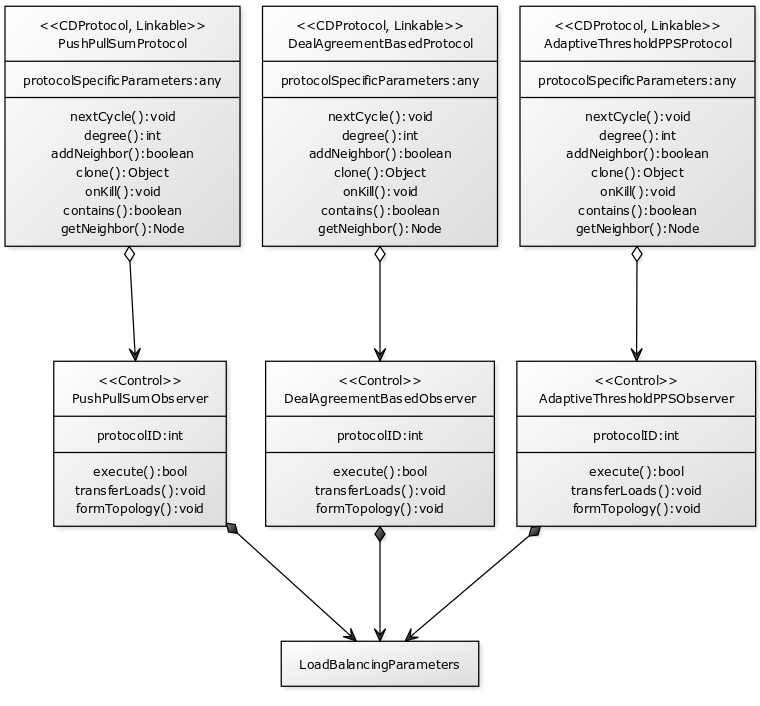
\includegraphics{figures/Diagrams/projectUML.png}}
    \caption{Project structure}
    \label{fig:uml}
\end{figure}

\section{Implementation Details}\label{sec:implementationdetails}
Figure \ref{fig:ProcessModel} depicts a process model, modeling the method chosen to transition from experiment creation to data analysis and visualization. The methodology follows three steps. First, I wrote a Python script that generates configuration files where each node has uniformly distributed random load/sum values. 30 distinct experiments were created to improve statistical significance. Then a Java script reads these configuration files and assigns an initial load value to each node. After that the simulations are conducted. Each simulation outputs a file containing the simulation results, mainly the MSE per round, the loads per round, and the configuration of the network (e.g., which topology is chosen, network size, etc.). The simulation results are averaged per round and then analyzed. Out of the simulation results, plots are generated, showing the MSE reduction per round in log-log or log-linear graphs. Additionally, model-fitting techniques are applied to further analyze trends in the data.

\begin{figure}
    \centering
    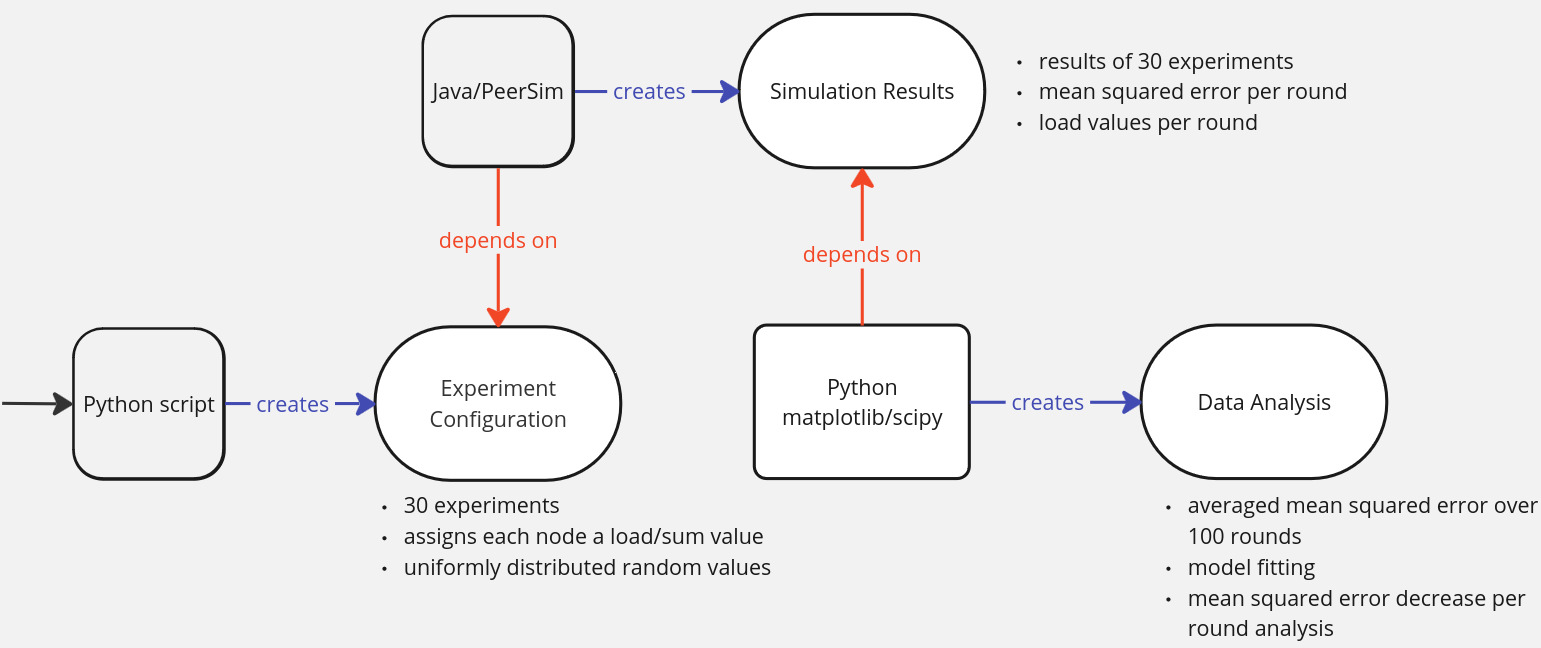
\includegraphics[width=\textwidth]{figures/Diagrams/process_model.png}
    \caption{Process model: methodic}
    \label{fig:ProcessModel}
\end{figure}
    \chapter{Simulation Outcomes}\label{chap:simulationoutcomes}
When analyzing load balancing algorithms, the stability and efficiency of the algorithms are considered. Stability refers to how well an algorithm balances any initial load distribution across a network \cite{ChengzhongFrancis}. In the following, this is tested. 1. by conducting 30 independent experiments for each topology, each with different initial load values per node 2. by choosing six distinct topologies (some with varying structural symmetry, e.g., $L_{32,32}$, $L_{128,8}$, and $L_{8,128}$) to test the performance of the load balancing algorithms. Efficiency measures how fast an algorithm achieves a balanced state in the network. To test this, the MSE is chosen as a metric and compared over the rounds to see which algorithm achieves low error values faster. A lower MSE at an earlier stage indicates higher efficiency. For clarity, the load balancing algorithms are abbreviated:

\textbf{DAB - Single-Proposal Deal-Agreement-Based Algorithm}

\textbf{PPS - Push-Pull Sum Algorithm (classic or traditional PPS)}

\textbf{ATPPS - Adaptive Threshold Push-Pull Sum Algorithm (adaptive PPS)}

The simulation outcomes are presented in log-log or log-linear graphs (logs for the MSE data are base 10), since the MSE varies significantly over the 100 simulation rounds. Each simulation outcome includes an analysis of the slopes for three regions of the x-axis (simulation rounds) and the overall slope computed across all 100 rounds. The MSE data over time is modeled using linear regression, polynomial regression, exponential regression, or logarithmic regression, depending on the best-fitting model.

\textbf{Linear Regression}: Linear regression models the relationship between MSE and simulation rounds as $$MSE_r=m*r+b,$$ where $m$ is the slope, calculated as $m=\frac{\Delta MSE}{\Delta r}=(\frac{MSE_{r_2}-MSE_{r_1}}{r_2 - r_1})$. In this context the slope is mostly negative, as $MSE_r$ decreases in comparison to $MSE_{r-1}$. $b$ is the initial MSE at round $r=0$, which represents the initial imbalance of the network before any load balancing is applied.

\textbf{Polynomial Regression}: The polynomial regression model is expressed as $$MSE_r=a_0+a_1*r+a_2*r^{2}+a_3*r^{3}+...+a_n*r^{n}.$$ This model is utilized when MSE reduction per round follows a power law relationship. It captures non-linear relationships between the independent variable $r$ and dependent variable $MSE_r$ \cite{MotulskyDataFitting}. Polynomial regression can model non-linear trends like diminishing returns (e.g., rapid MSE reduction initially, then slower reduction). It fits the curvature of MSE decay, even if it's not strictly exponential or linear. Higher-degree polynomials can capture intricate patterns in the reduction of MSE over rounds.

\textbf{Exponential Regression}: The exponential regression model is given by $$MSE_r=a*e^{-br}.$$ Exponential models capture the initially steep drop in MSE at early rounds, followed by slower reductions in later rounds. $a$ represents the initial MSE value. A larger $a$ indicates a higher initial load imbalance in the network. $b$ is the decay rate; it captures how quickly the MSE decreases per round $r$. Since MSE decreases over time, $b$ is negative. A larger negative value for $b$ indicates a faster error reduction in the network, thus a faster convergence, while values closer to 0 indicate slower error reduction.

\textbf{Logarithmic Regression}: The logarithmic regression models data as $$\log{(MSE_r)}=a+b*\log{(r)},$$ where $a$ is the initial MSE when $\log{(r)}=0$ and $b$ is the rate of reduction per unit increase in $\log{(r)}$. A large positive $b$ decreases the MSE faster. If $b$ is small, the error reduction slows down as the rounds progress.This model is effective in analyzing load balancing algorithms where initial rounds see significant MSE reductions, followed by progressively smaller improvements.

\section{Complete Graph}\label{sec:completeGraph}

\begin{figure}[]
    \centering
    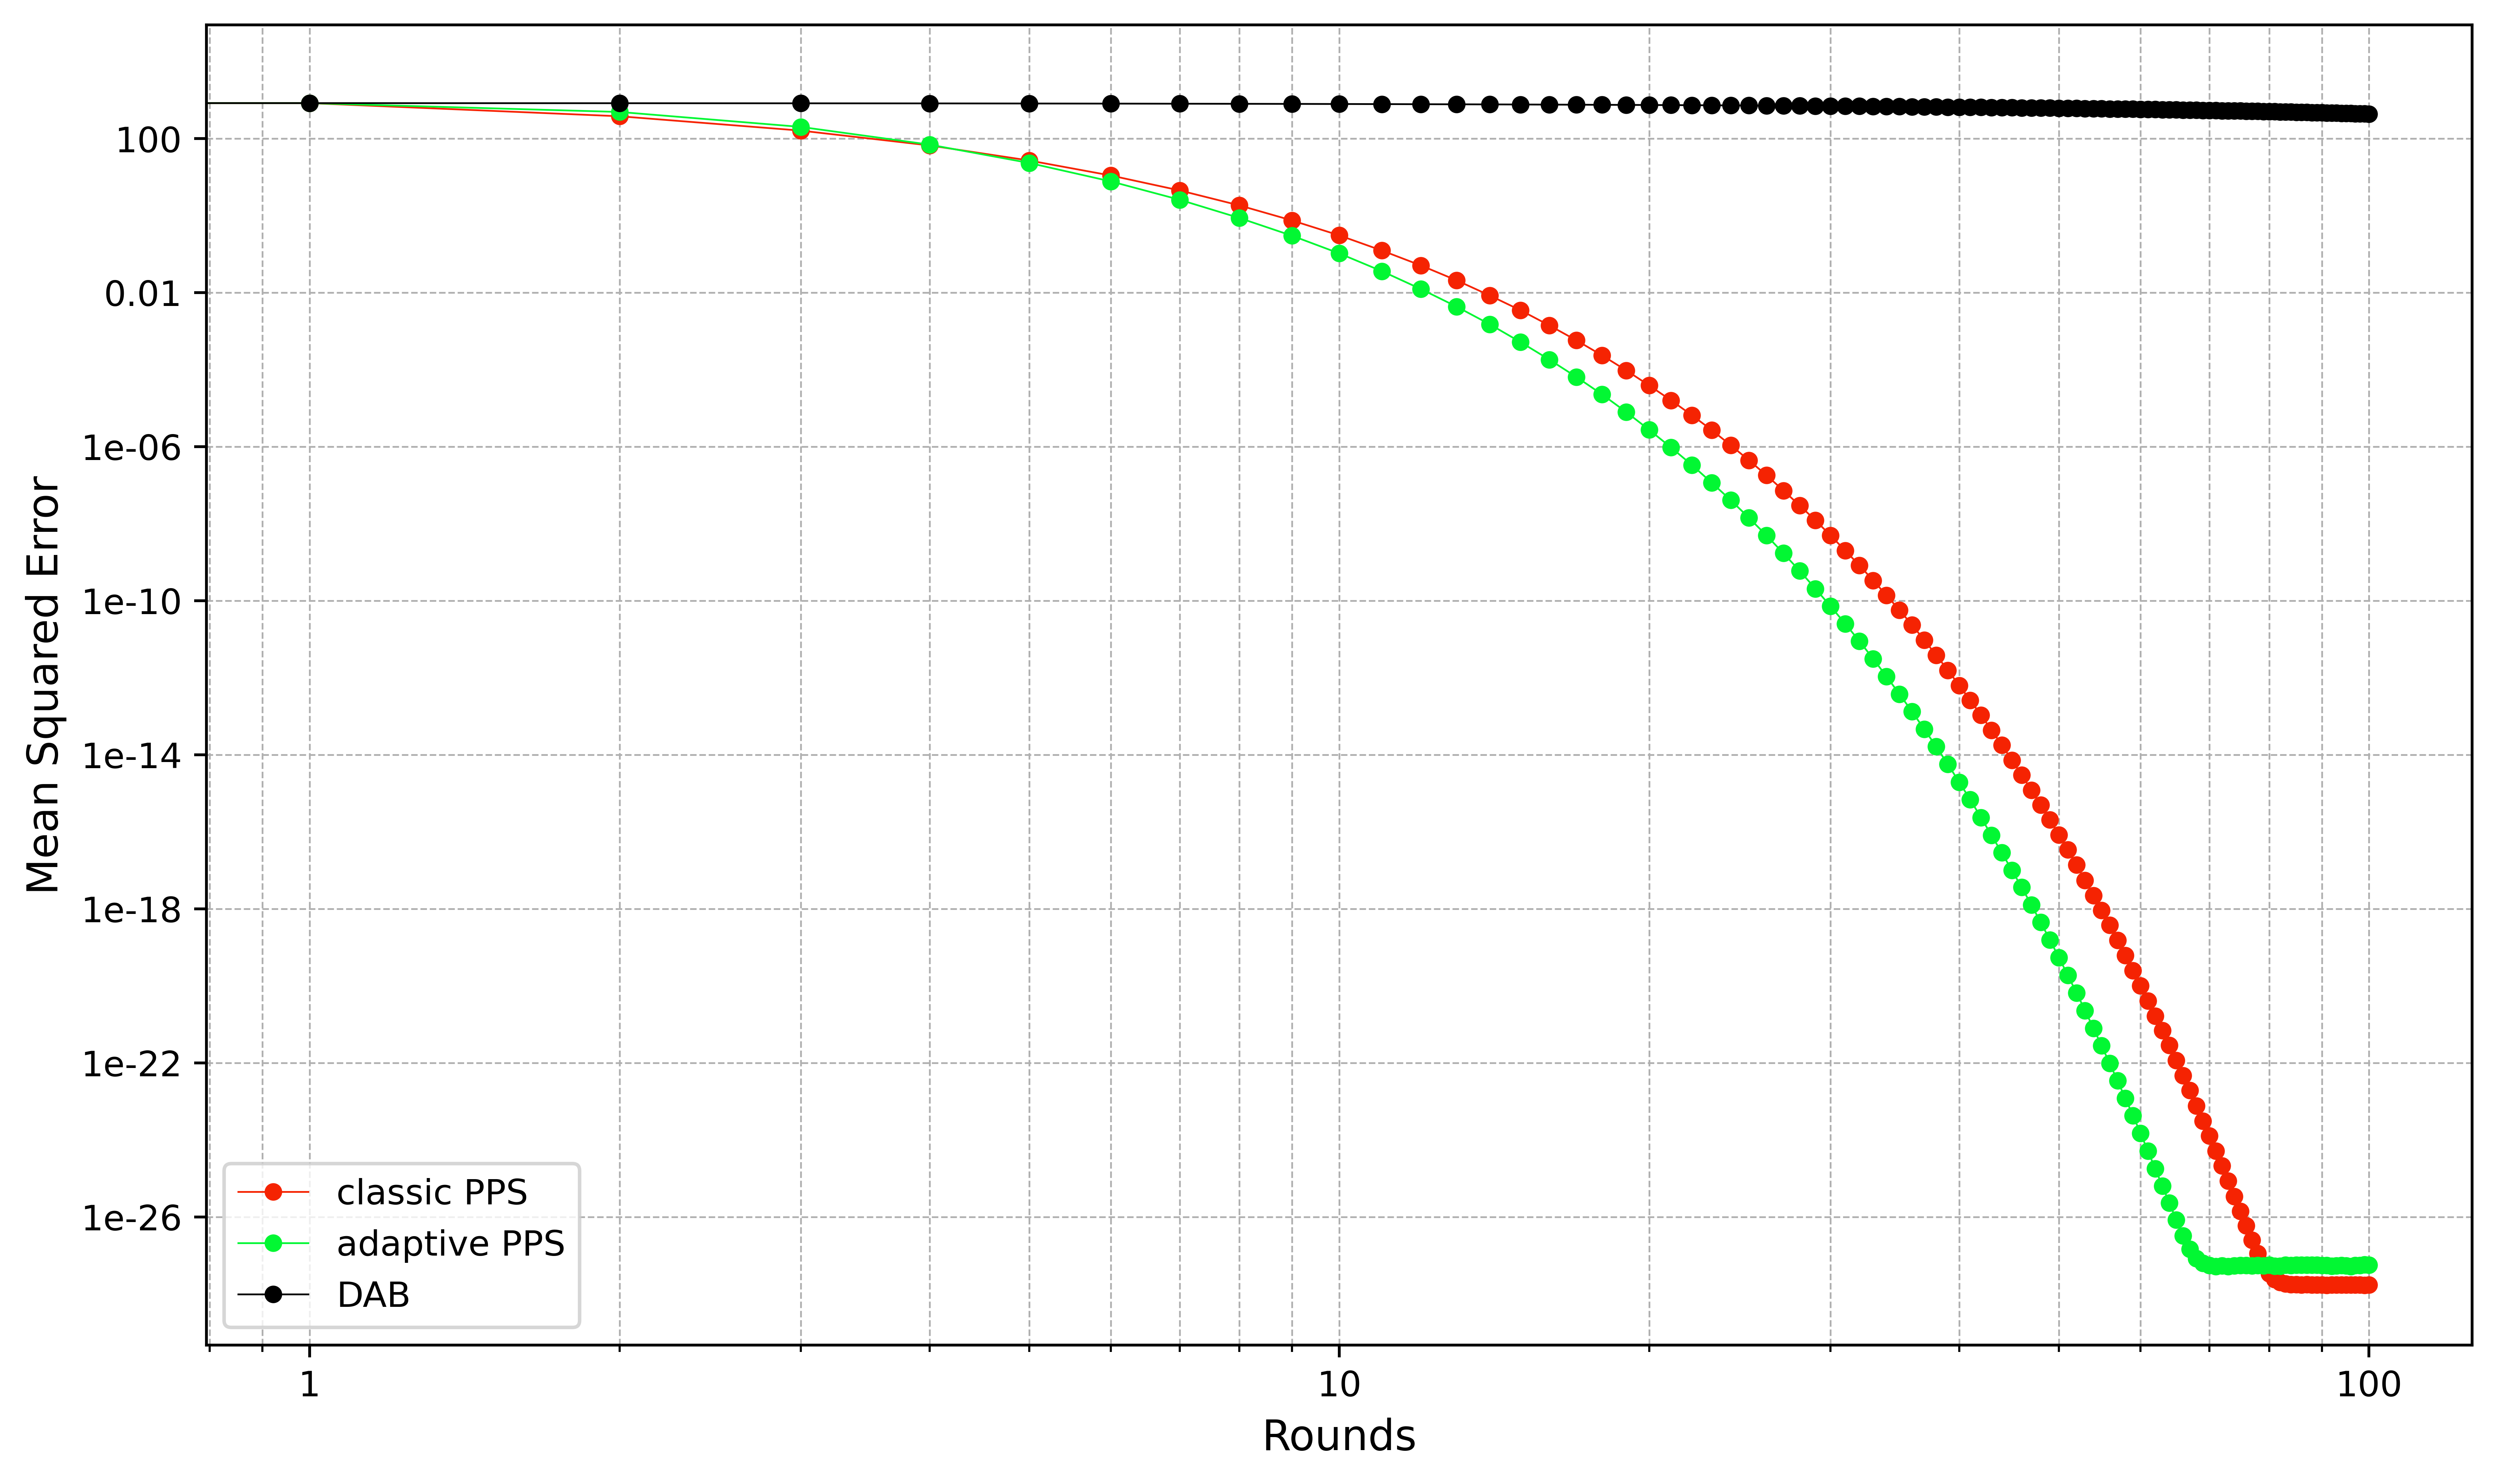
\includegraphics[width=\linewidth]{figures/Simulation_outcomes/CompleteGraph/DAB_vs_PPS_CG_r100_n1024_averaged_loglog.png}
    \caption{Complete graph: mean squared error per rounds (log-log)}
    \label{fig:completegraphMSEperRoundLogLog}
\end{figure}

Figure \ref{fig:completegraphMSEperRoundLogLog} presents the MSE reduction per round for the three load balancing algorithms simulated on the Complete graph on a log-log graph. The DAB curve (black curve) shows a linear trend and a gentle decrease of the MSE over the 100 rounds. The DAB performs poorly since it uses a fixed, deterministic load redistribution rule for its nodes, where each node selects the minimally loaded neighbor and proposes a load transfer. In a Complete graph where each node is interconnected, the same few nodes that hold the load of amount $L_{min}$ are the nodes that are receiving all the proposals. Since each minimal neighbor only accepts one proposal per round, the number of load transfers is heavily limited, resulting in slow MSE reduction. The PPS and ATPPS algorithms leverage the high connectivity of the network more effectively, due to their randomized nature. The PPS curve (red curve) exhibits a steady decrease in MSE, therefore showing efficient MSE reduction over time. Since all nodes are equally connected, no structural constraints slow down the process of pushing and pulling loads from neighbors. However, PPS does not distinguish between nodes that are highly imbalanced and those that are nearly balanced, leading to unnecessary load transfers in later rounds, which slows convergence. The ATPPS algorithm (green curve) achieves even faster MSE reduction than PPS. As the system nears equilibrium, ATPPS reduces redundant exchanges, causing the red curve to stagnate after a certain point in time. In summary, DAB underperforms due to limitations on the amount of load transfers; PPS improves upon this but lacks adaptive control, while ATPPS optimally balances load while avoiding unnecessary exchanges, making it the most effective approach in this setting.

Figure \ref{fig:dabCompleteModelFit} shows the exponential regression fit for the MSE data when the DAB algorithm as a load balancing algorithm is applied to the network. Even though the curve might not suggest an exponential decay, the MSE data fits with the exponential regression model following the equation $MSE_r=844.63*e^{-0.01*r}$. The decay rate of -0.01 suggests a very slow decrease in MSE. The fitted curve and model seem very suitable for the MSE data, since the fitted curve aligns with the MSE data. The MSE data of the PPS is fitted to the exponential regression model for rounds 10 to 80. Over time, repeated randomized exchanges smooth out load imbalances, leading to an exponential decay in MSE, as seen in figure \ref{fig:ppsCompleteModelFit}. The best fit follows the equation $MSE_r=2530.41*e^{-0.9*r}$. In Figure \ref{fig:atppsCompleteModelFit}, the exponential regression fit is visualized for the MSE data of the ATPPS load balancing algorithm graph in the complete graph for rounds 10 to 65. The fitted curve is expressed by the equation $MSE_r=4309.94*e^{-1.06*r}$. A steep error reduction is indicated by the decay rate of -1.06. As the PPS algorithm, the ATPPS algorithm reduces the error very effectively in an exponential manner. Rounds 66 to 100 show a plateauing of the MSE data. The adaptive mechanism provides a faster decline in error indicated by the decay rate of -1.06 versus the one of the PPS of -0.9.

Figure \ref{fig:completegrapslopes} visualizes a heat map of the slopes (rates of change) for the three load balancing algorithms across different regions of the graph. The values reflect how steeply the MSE decreases over rounds. PPS and ATPPS have steep negative slopes in the start region, rounds 1-10 with a value of -92, indicating rapid initial improvement. However, their slopes in the middle (rounds 11-65) and end regions (rounds 66-100) approach zero, suggesting a plateau in performance. DAB has shallower negative slopes overall, reflecting a more gradual and consistent error reduction across all regions. The general slopes (rounds 1-100) for PPS and ATPPS (-8.4) are much steeper than DAB (-4.4), suggesting that PPS and ATPPS converge faster on average. The end region is chosen as 66-100 to catch the trend of plateauing for the ATPPS and also for PPS, which is beginning to plateau in error reduction in later rounds (rounds 80-100). The MSE is reduced significantly by the PPS and ATPPS. The initial MSE value of $832$ is reduced to $1.72 \times 10^{-28}$ for the PPS and $5.63 \times 10^{-28}$ for the ATPPS, while the DAB reduced the error to nearly half of the initial value, achieving a value of $436.84$.

\begin{figure}[]
    \centering
    \scalebox{0.8}{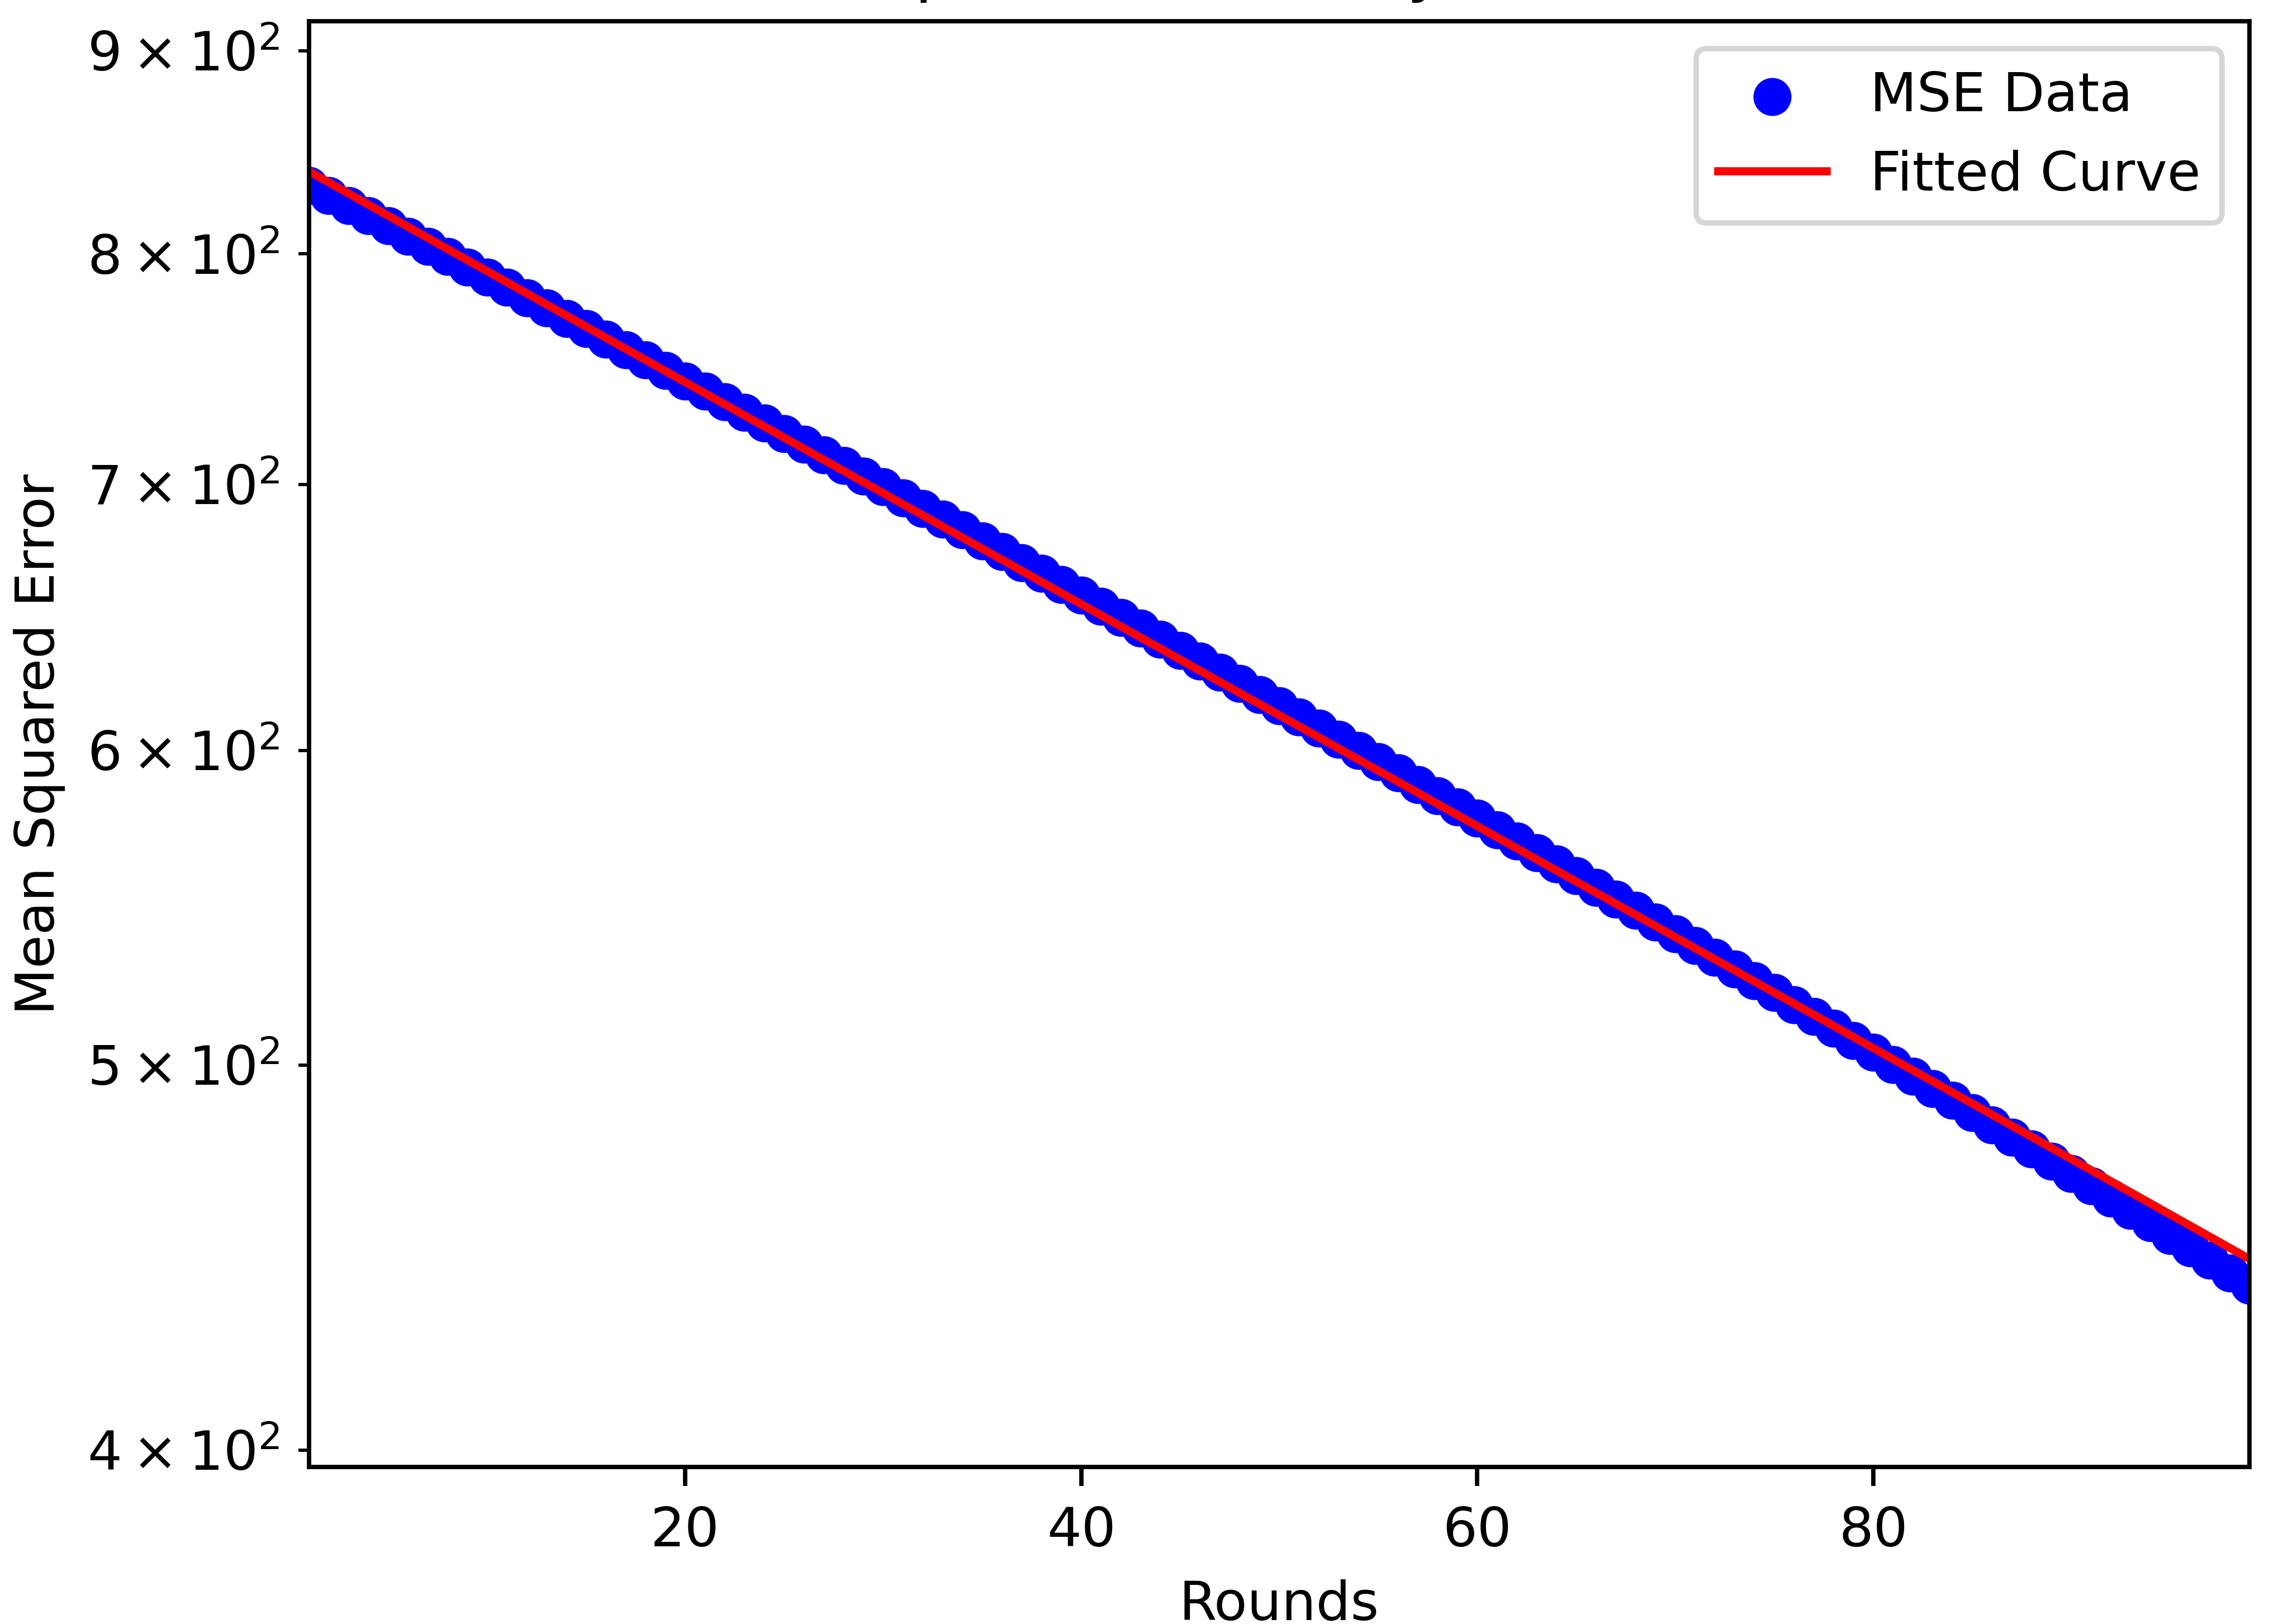
\includegraphics{figures/Simulation_outcomes/CompleteGraph/DAB/DAB_modelfitting_rounds_99_model_1.png}}
    \caption{Complete graph - exponential regression fit: DAB}
    \label{fig:dabCompleteModelFit}
\end{figure}

\begin{figure}[]
    \centering
    \scalebox{0.8}{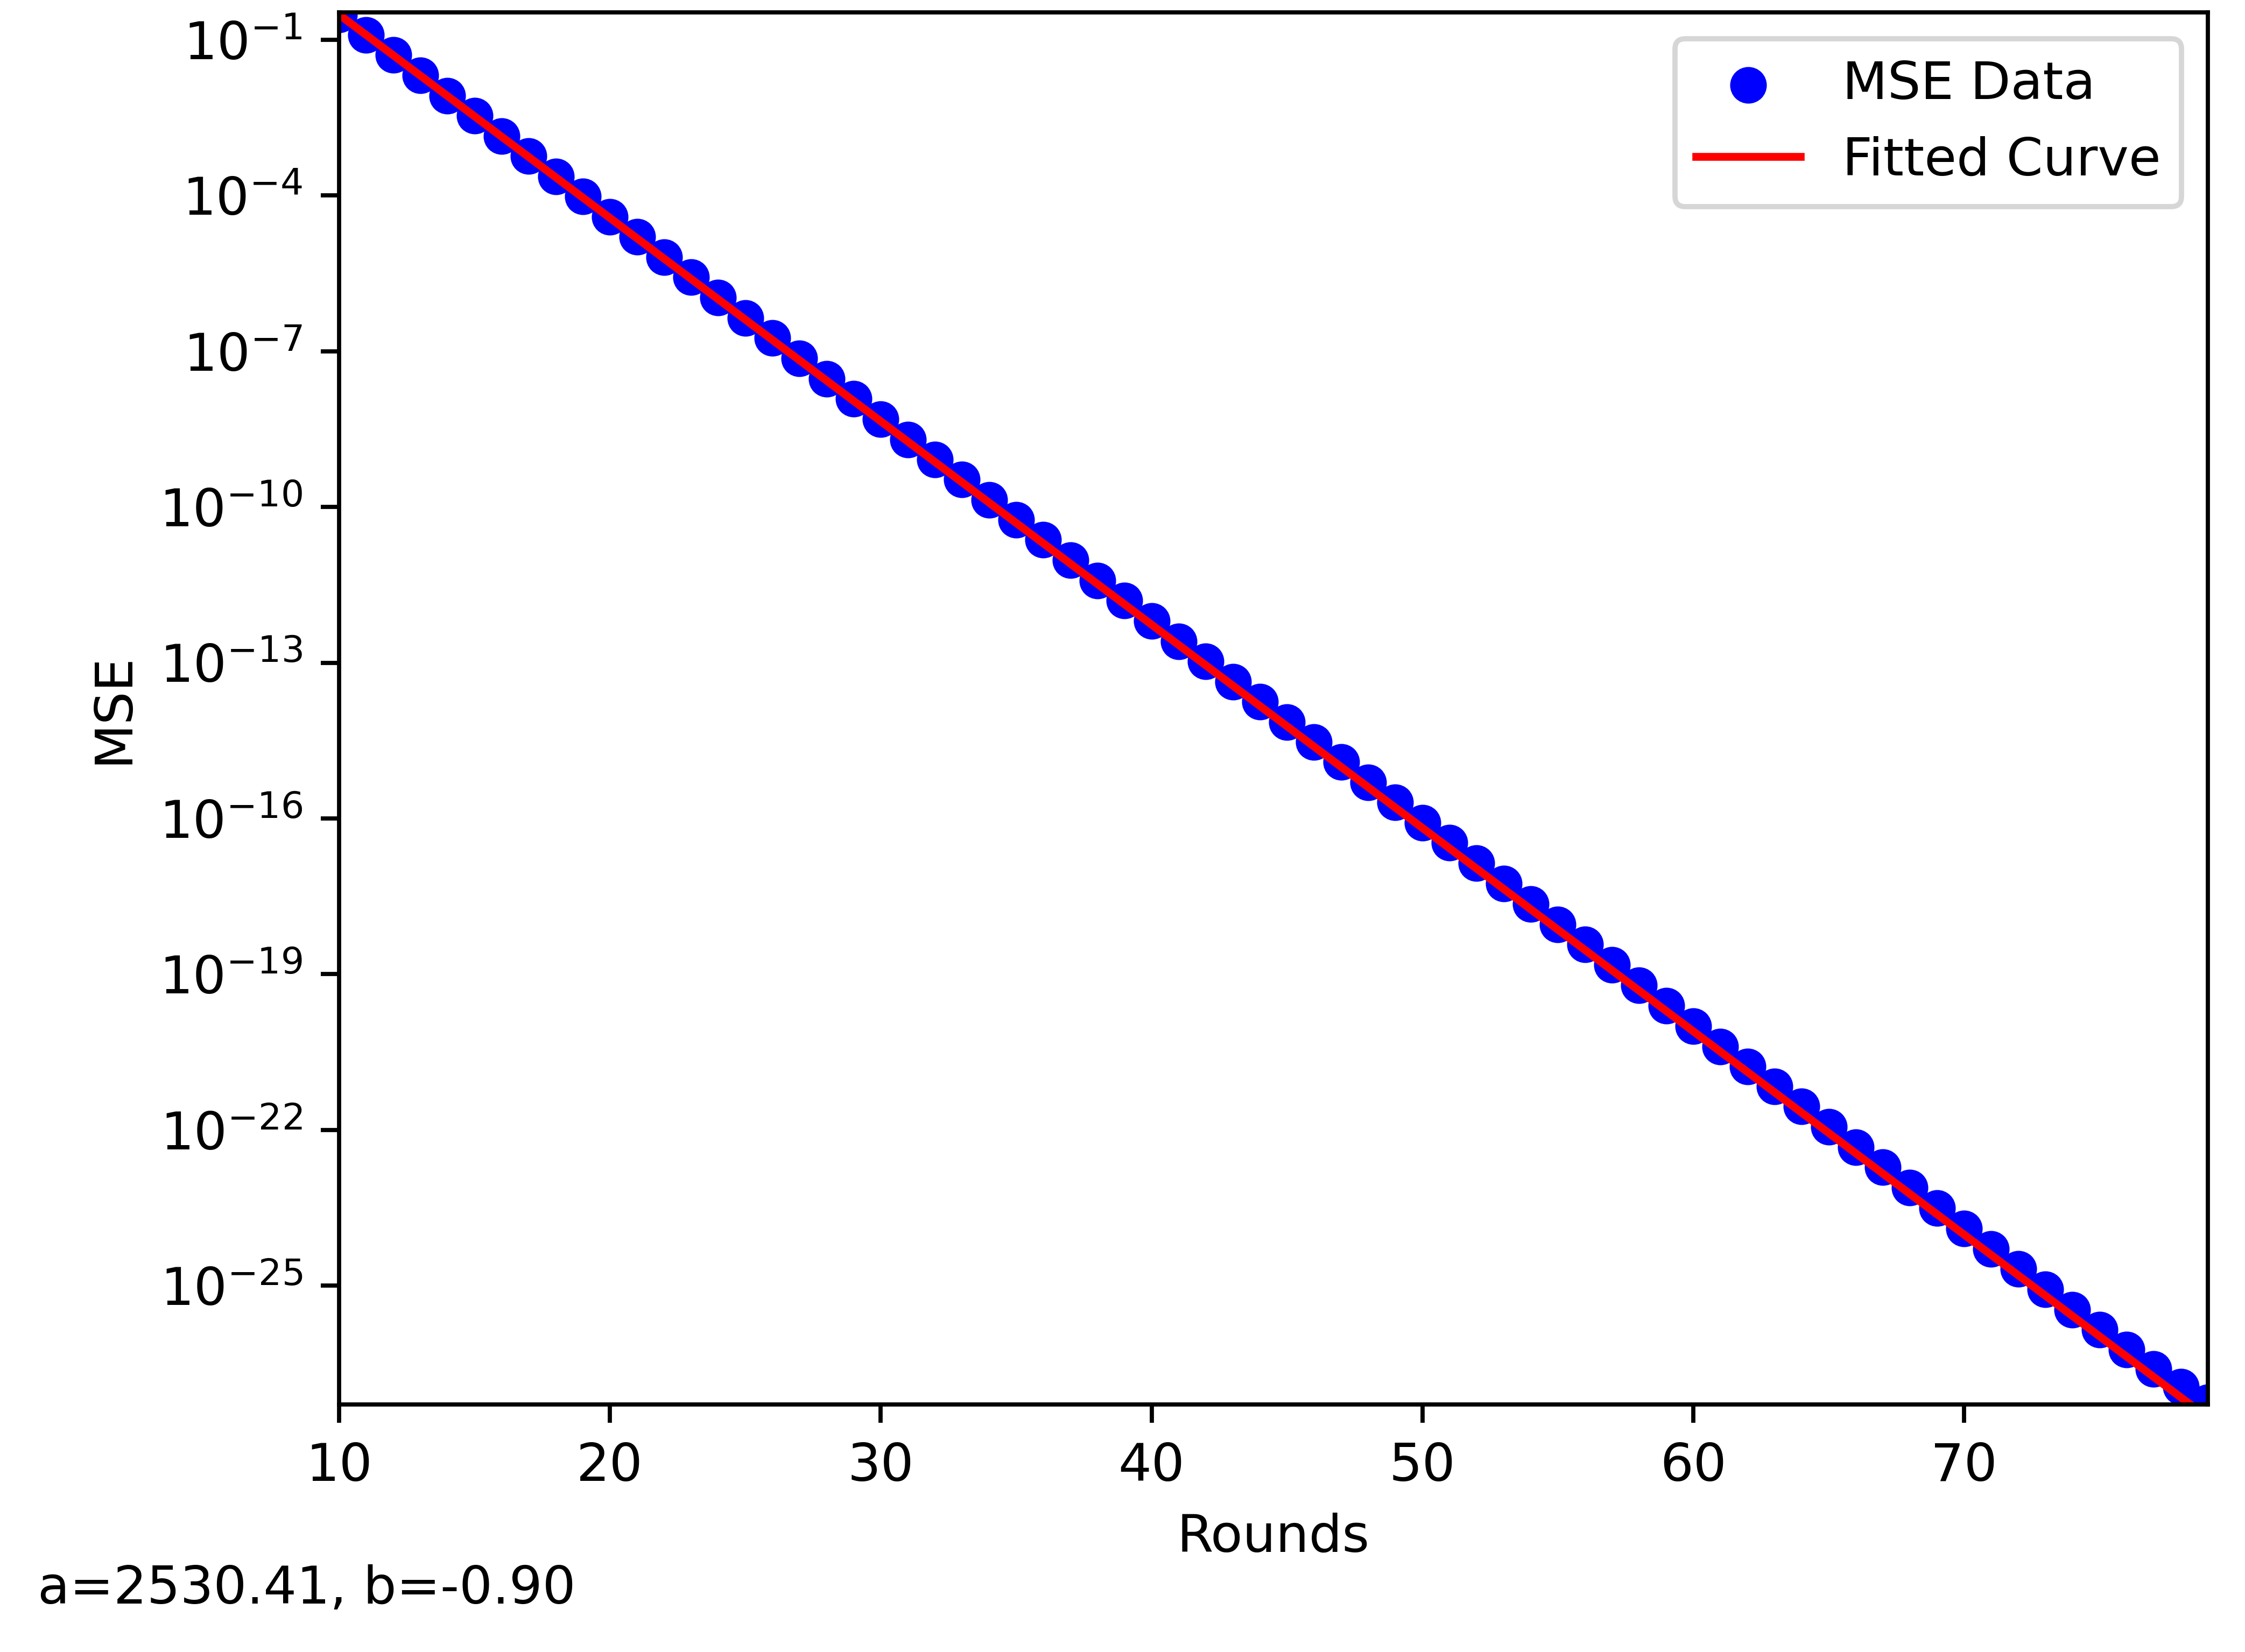
\includegraphics{figures/Simulation_outcomes/CompleteGraph/PPS/PPS_modelfitting_rounds_79_model_1.png}}
    \caption{Complete graph - exponential regression fit: PPS}
    \label{fig:ppsCompleteModelFit}
\end{figure}

\begin{figure}[]
    \centering
    \scalebox{0.8}{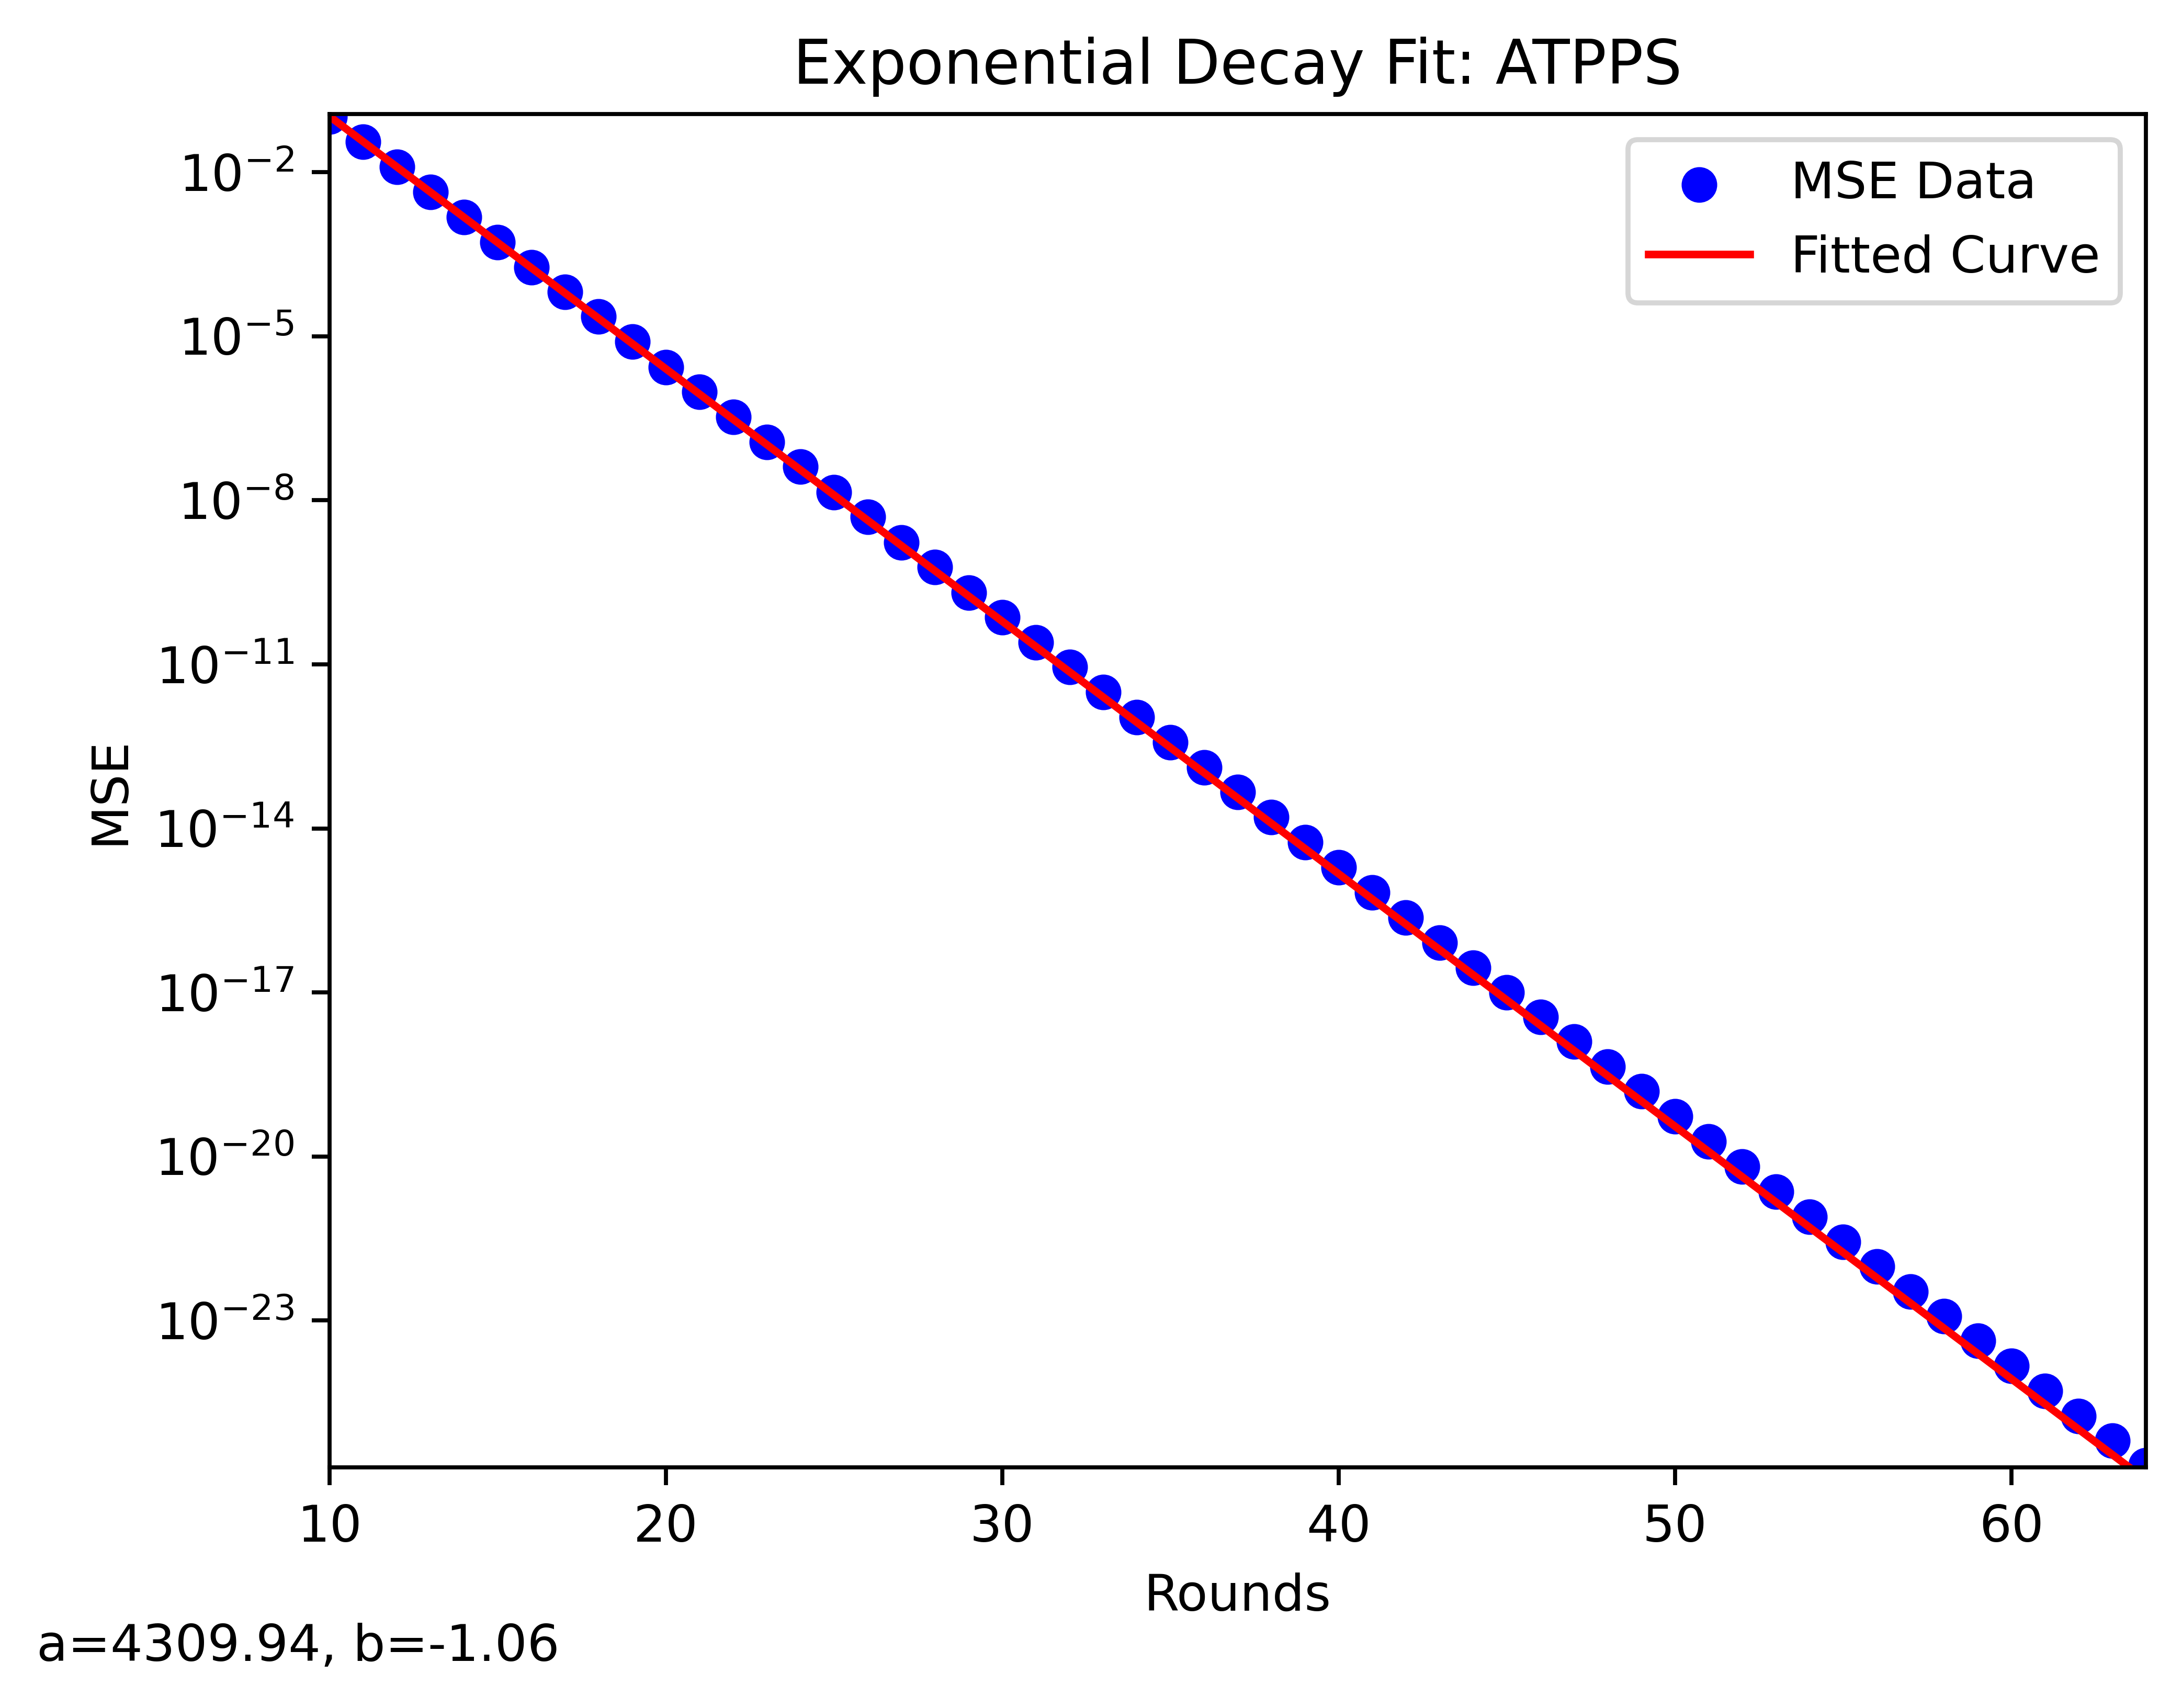
\includegraphics{figures/Simulation_outcomes/CompleteGraph/ATPPS/ATPPS_modelfitting_rounds_64_model_1.png}}
    \caption{Complete graph - exponential regression fit: ATPPS}
    \label{fig:atppsCompleteModelFit}
\end{figure}

\begin{figure}
    \centering
    \scalebox{0.8}{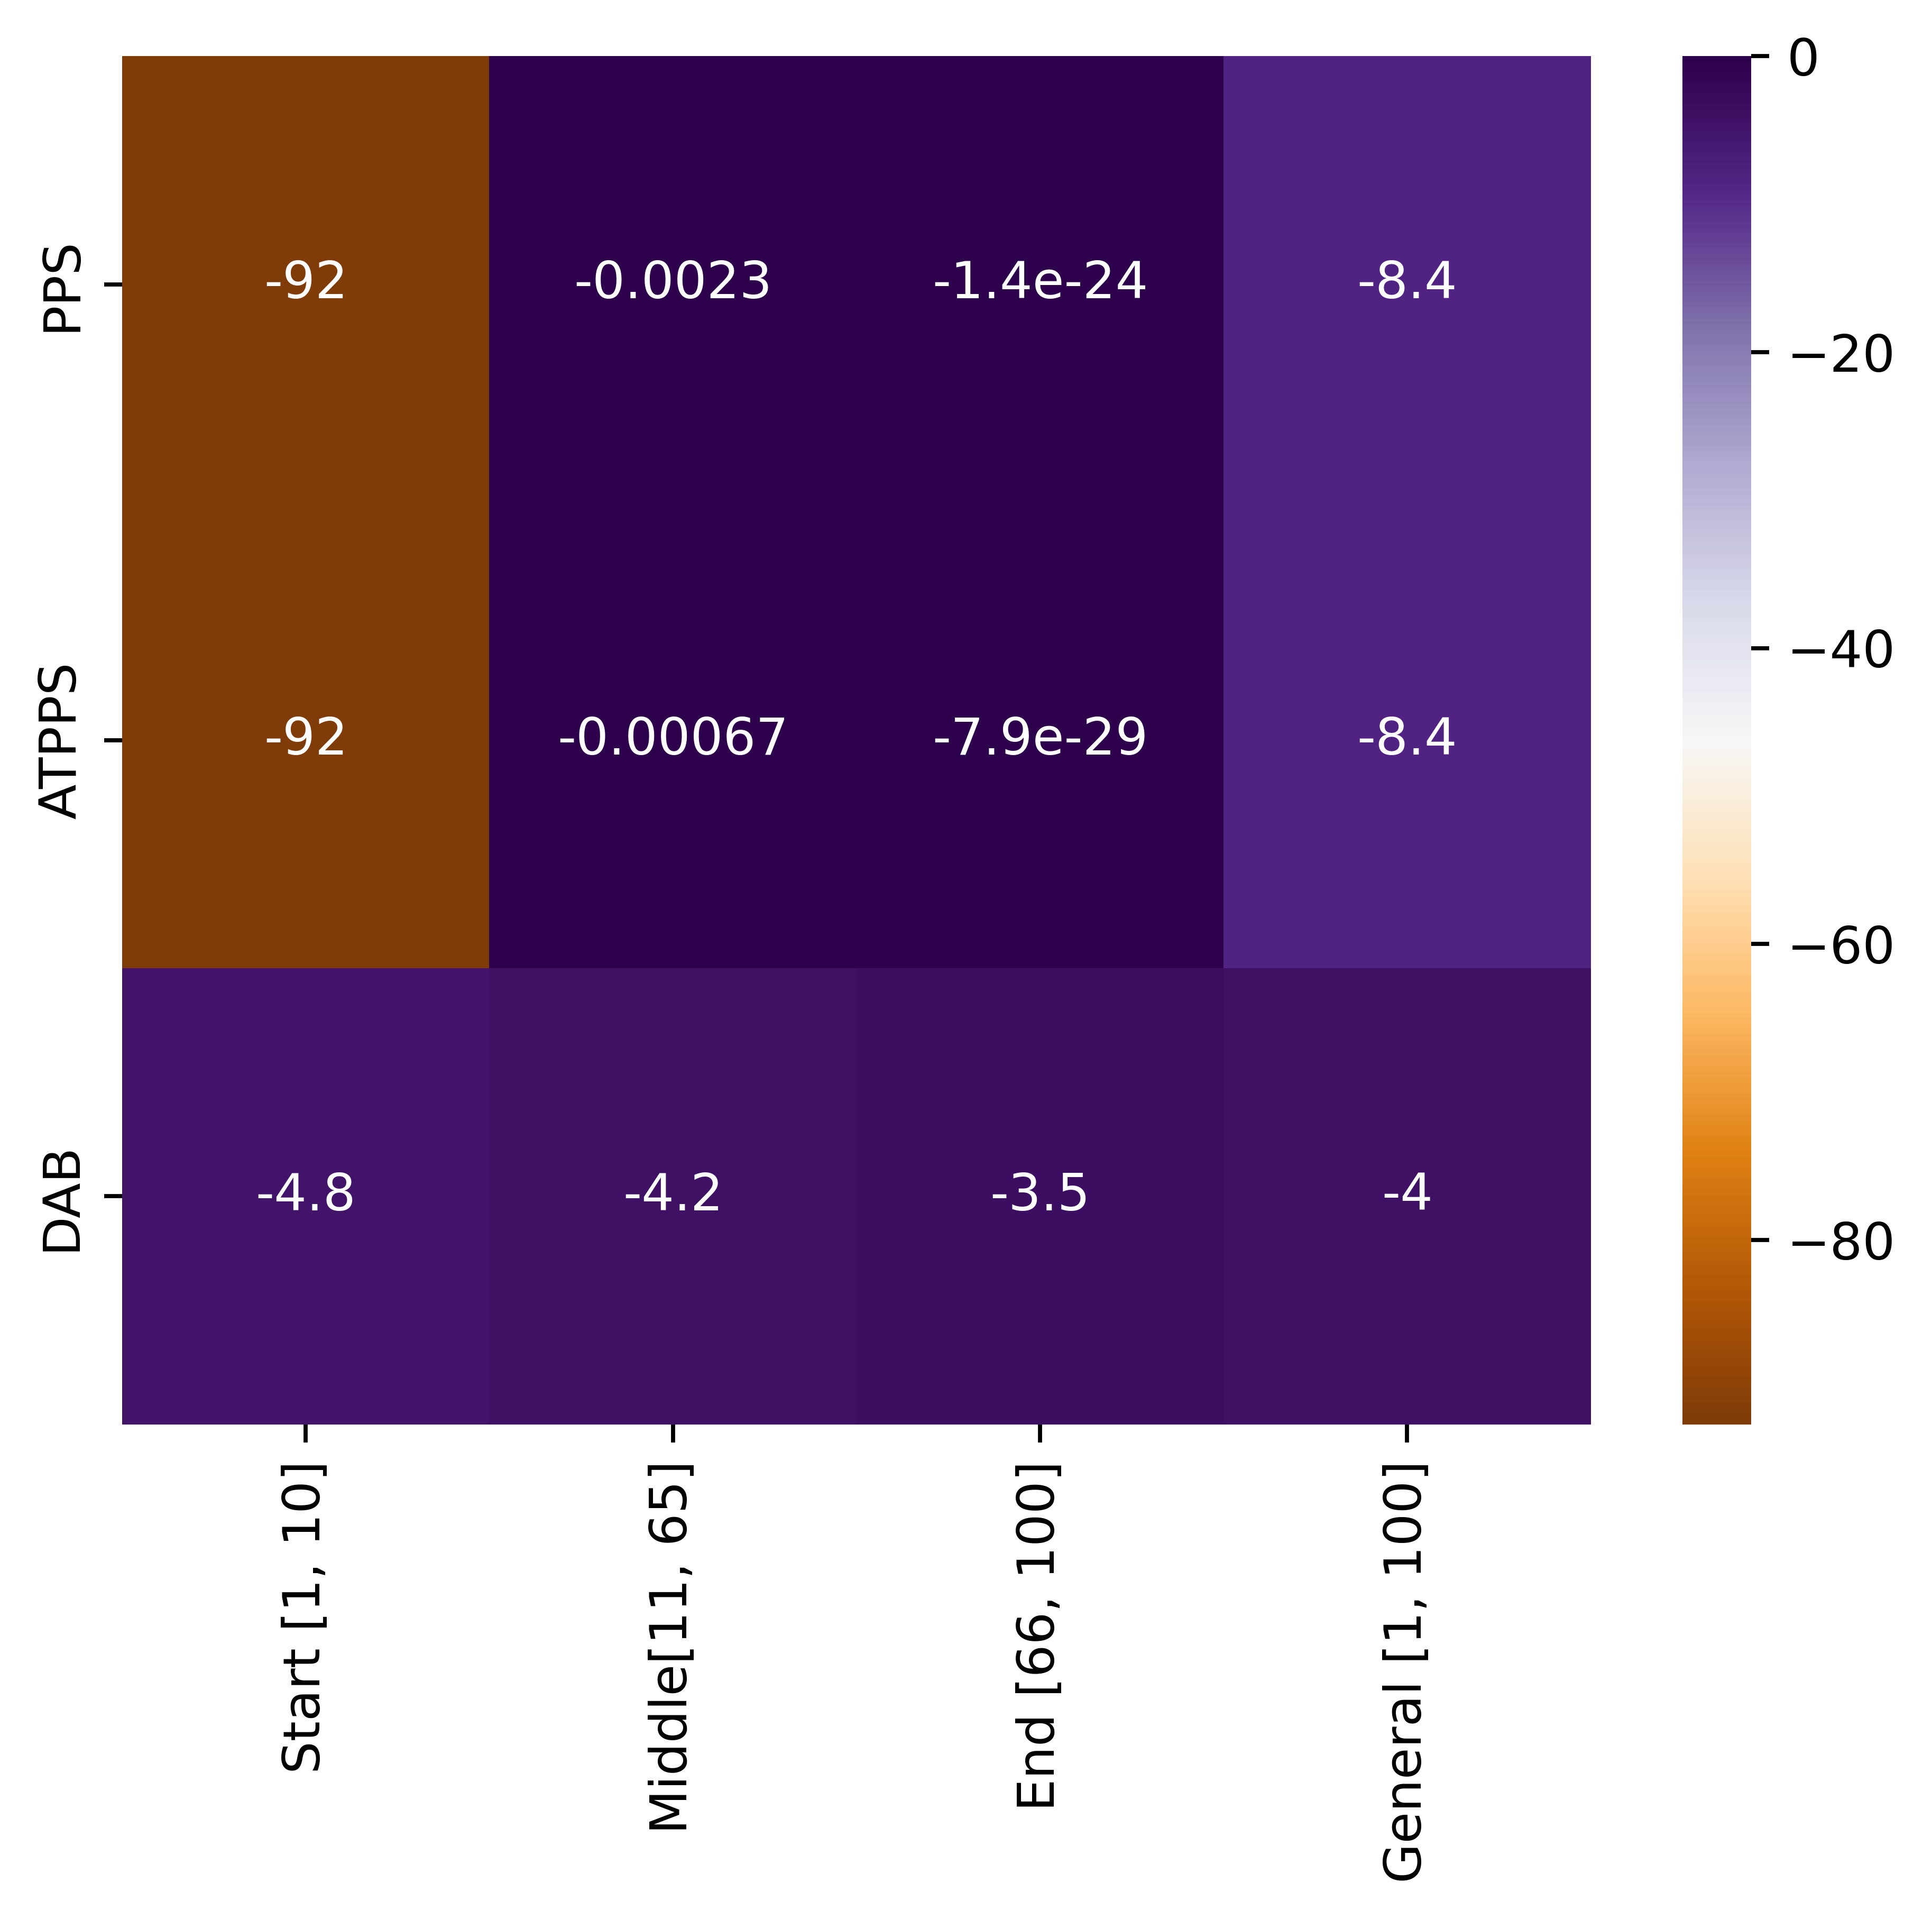
\includegraphics{figures/Simulation_outcomes/CompleteGraph/DAB_vs_PPS_vs_ATPPS_slopesheatmap_100rounds.png}}
    \caption{Complete graph: heat map of slopes per region}
    \label{fig:completegrapslopes}
\end{figure}

\section{Star Graph}\label{sec:stargraph}
The behavior of the curves in figure \ref{fig:stargraphMSEperRoundLogLog} is similar to those for the Complete graph, with the difference that the PPS curve falls more steeply than the ATPPS curve. Again, DAB shows a much slower MSE reduction compared to PPS and ATPPS, as indicated by the flatter slope of its curve. It converges minimally, with MSE remaining nearly constant over rounds after an initial reduction. This indicates that DAB is less efficient in balancing load in a Star graph, likely due to its deterministic nature and lack of dynamic adaptability. In the Star graph, all the leaves have the central node as a partner, meaning each leaf node selects the same central node to propose load transfers. When the central node has a higher load than the leaf requesting a transfer, no load transfer occurs between these two nodes, creating a bottleneck. Both PPS and ATPPS exhibit steep MSE reductions early on, as seen in the sharp downward trends in the log-log plot. The PPS algorithm balances load more efficiently than the ATPPS algorithm since it reduces MSE faster and reaches lower MSE values sooner (as of round 45) before the curve plateaus. The Push-Pull Sum based algorithms draw an advantage from the Star graph, as the redistribution happens through the central node, which is chosen by every leaf node as a push destination. Following that, the central node redistributes parts of the load to the leaf nodes in magnitude of $\frac{\frac{s_i,r}{2}}{N-1}$.

As seen in figure \ref{fig:dabStarModelFit} the MSE data for the DAB-balanced network aligns nearly perfectly with the fitted curve of the exponential regression model given by the equation $MSE_r=840.42*e^{-0.01*r}$ for the rounds 1 to 100, even though the decay rate of -0.01 indicates a very slow reduction in error. From round to round, the improvement in the network remains minimal. This highlights the inability of the DAB to balance the network within 100 rounds to a satisfactory level. Figures \ref{fig:ppsStarModelFit} and \ref{fig:atppsStarModelFit} show the fitted curves for the MSE data of the PPS and ATPPS algorithms, respectively. The best-fit model for the MSE data of the PPS load balancing algorithm between rounds 10 to 45 follows the equation $MSE_r=29794.60*e^{-1.39*r}$. The rounds 10 to 45 exhibit the steepest decline in MSE, and for that reason, they have been fitted to an exponential regression model. The decay rate of $-1.39$ indicates a rapid reduction in error, especially in comparison to DAB. For the ATPPS algorithm, the MSE data fits best with the exponential model in the range of rounds 18 to 60, following the equation $MSE_r=9329.40*e^{-1.05*r}$. In Star graphs, the central node dominates communication, and load balancing heavily depends on that node. Threshold-based adjustments do not significantly impact performance under these conditions. The discrepancy between the two PPS algorithms can be explained by the fact that the ATPPS limits the number of messages due to the conditional threshold-based load transfer, which means that there is less interaction compared to the PPS.

Overall, the situation is similar to the Complete graph, with the Push-Pull Sum-based algorithms performing an extremely quick error reduction and the DAB reducing the error exponentially at a very slow rate. This behaviour is captured in the heat map of figure \ref{fig:stargraphslopes}. While the DAB algorithm reduces the error with an average slope of $-3.75 \pm 0.55$ for the three regions, the Push-Pull Sum-based algorithms achieve an initial error reduction of approximately $-92$ within the first 10 rounds. The slopes approach zero in the middle and end regions, which implies negligible MSE reduction in later stages. This is because the network is already sufficiently balanced that later rounds will not see a noticeable improvement in the MSE. Both algorithms converge early and maintain a near-steady state afterward. The DAB's lack of adaptability leads to slower convergence and less effective load balancing, as reflected in its consistently shallow slopes. The MSE decreases from an initial value of $832$ to approximately $480.47$ for the DAB, while for the PPS and ATPPS algorithms, the MSE reaches values of $8.3\times 10^{-24}$ for the PPS and $\sim6.5 \times 10^{-24}$ for the ATPPS.

\begin{figure}[]
    \centering
    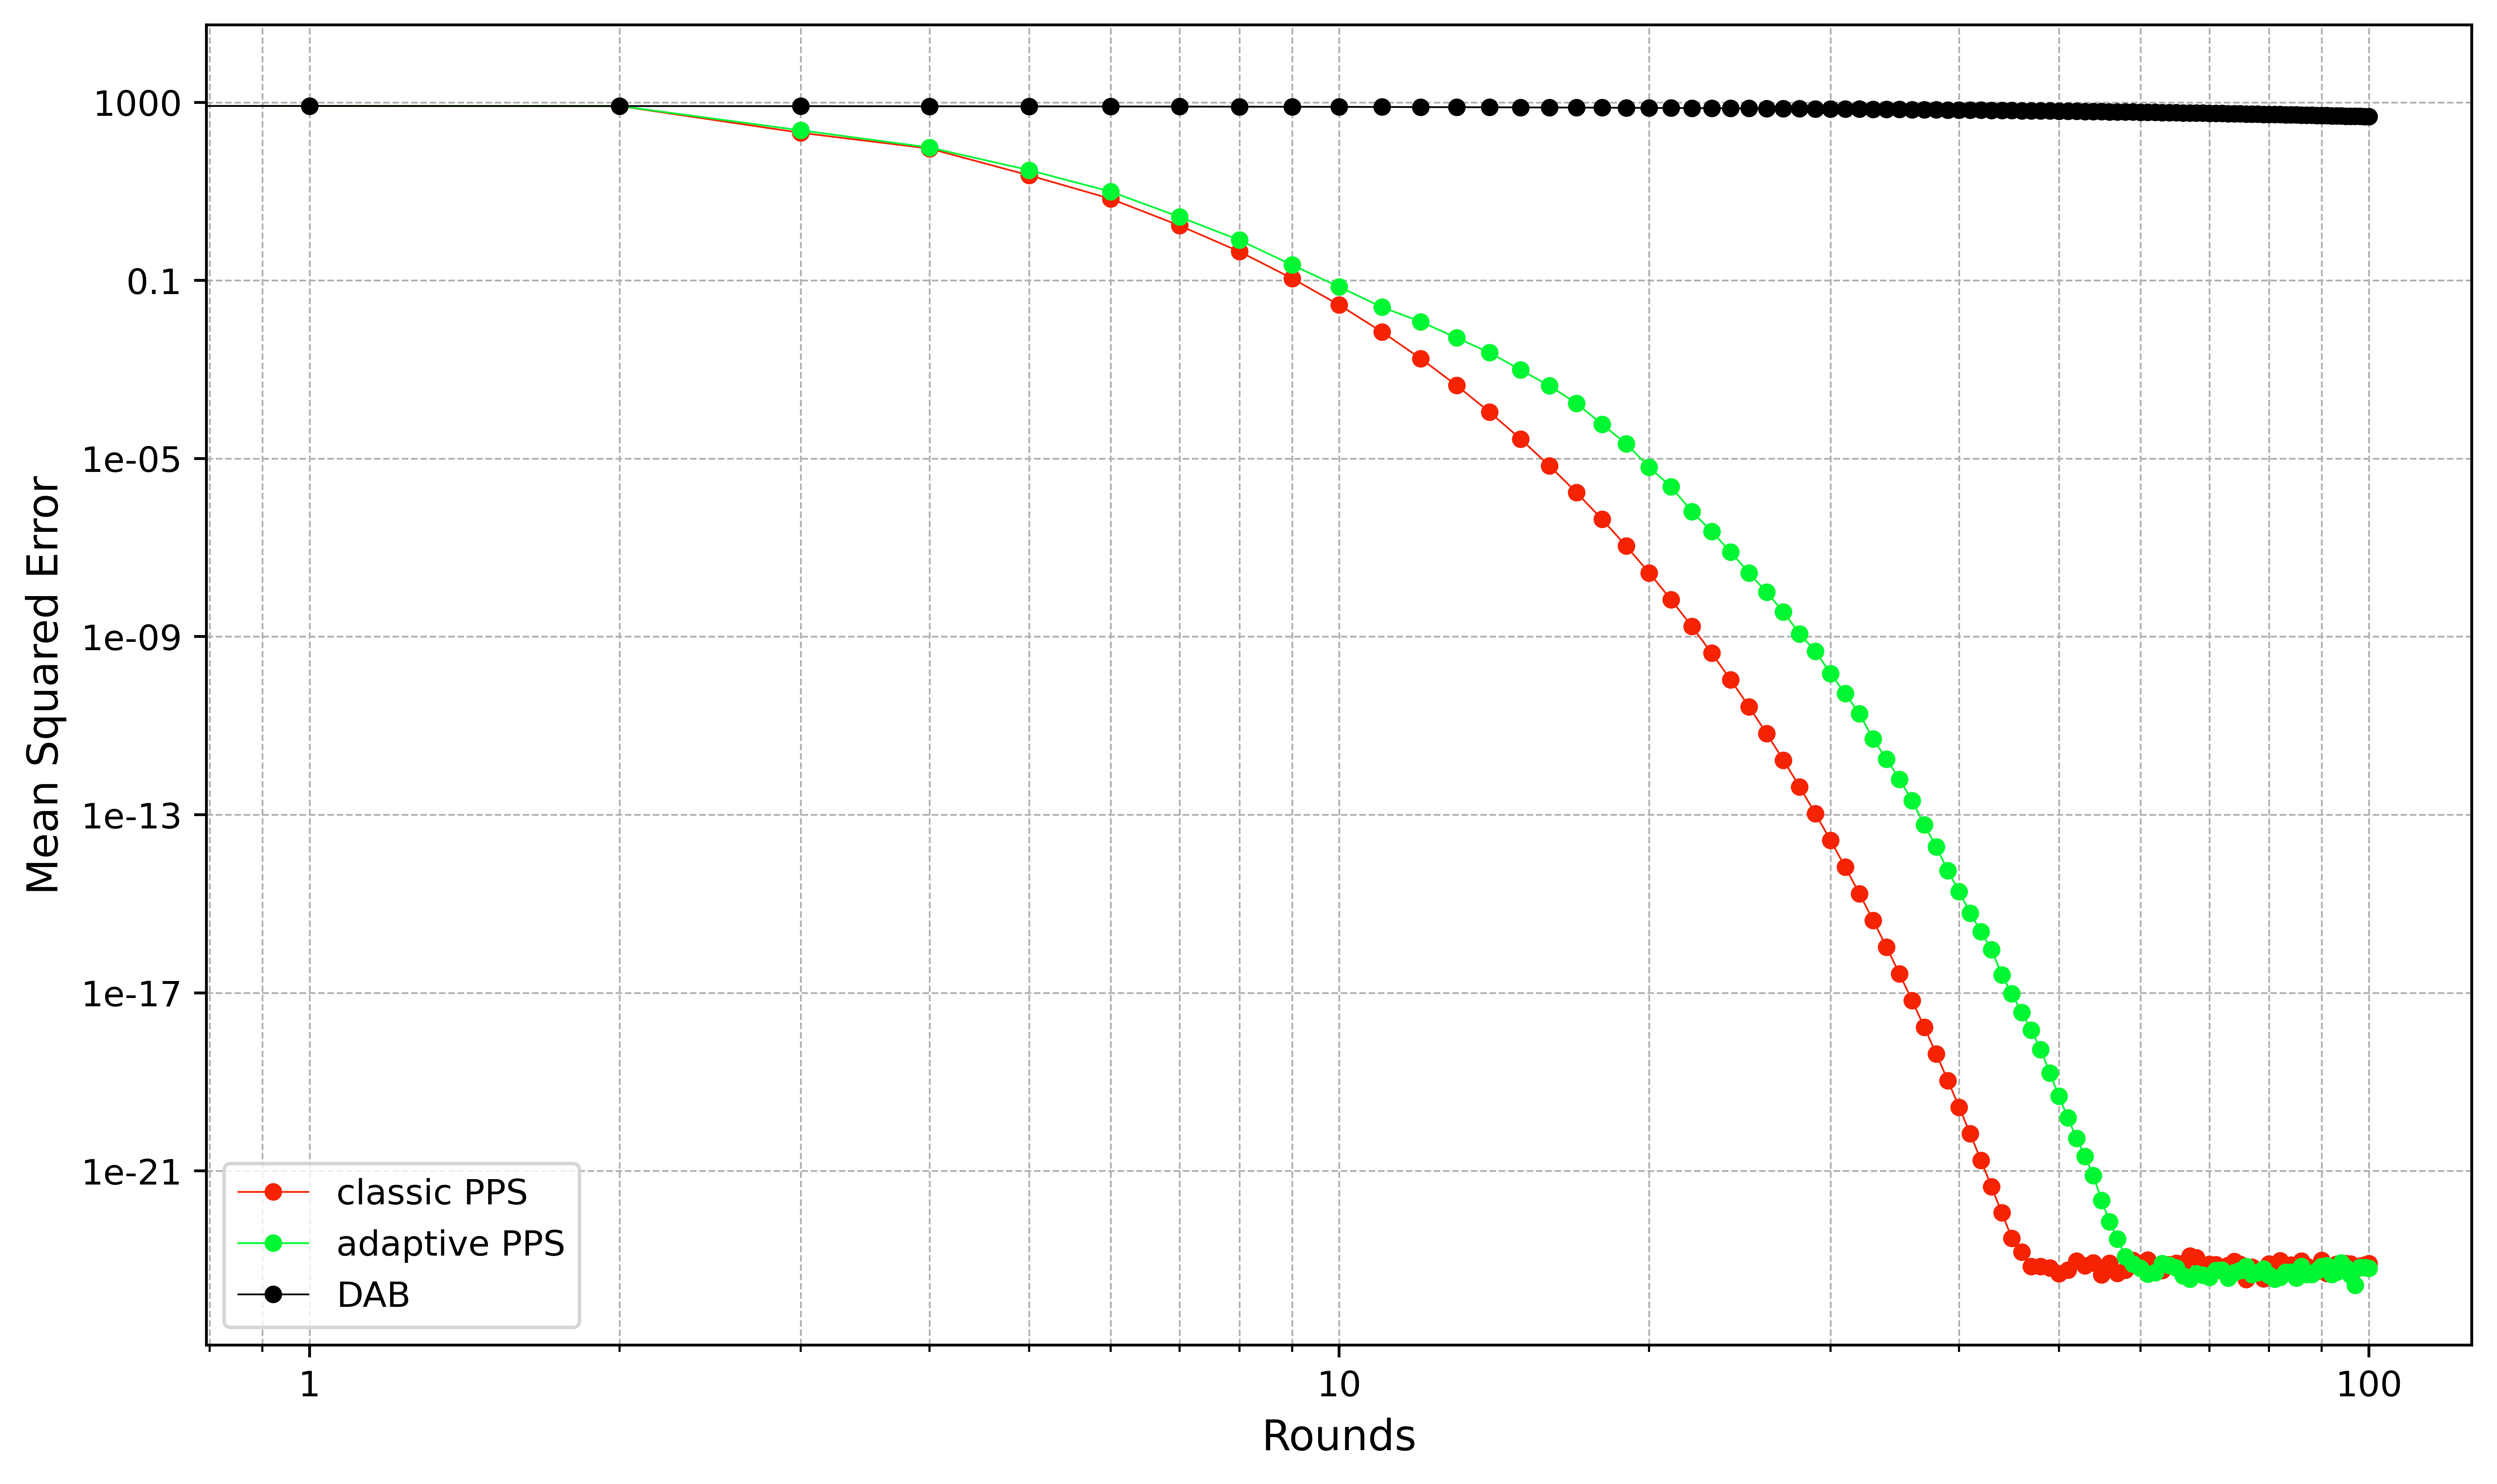
\includegraphics[width=\textwidth]{figures/Simulation_outcomes/StarGraph/DAB_vs_PPS_SG_r100_n1024_averaged_loglog.png}
    \caption{Star graph: mean squared error per rounds (log-log)}
    \label{fig:stargraphMSEperRoundLogLog}
\end{figure}
\begin{figure}[]
    \centering
    \scalebox{0.8}{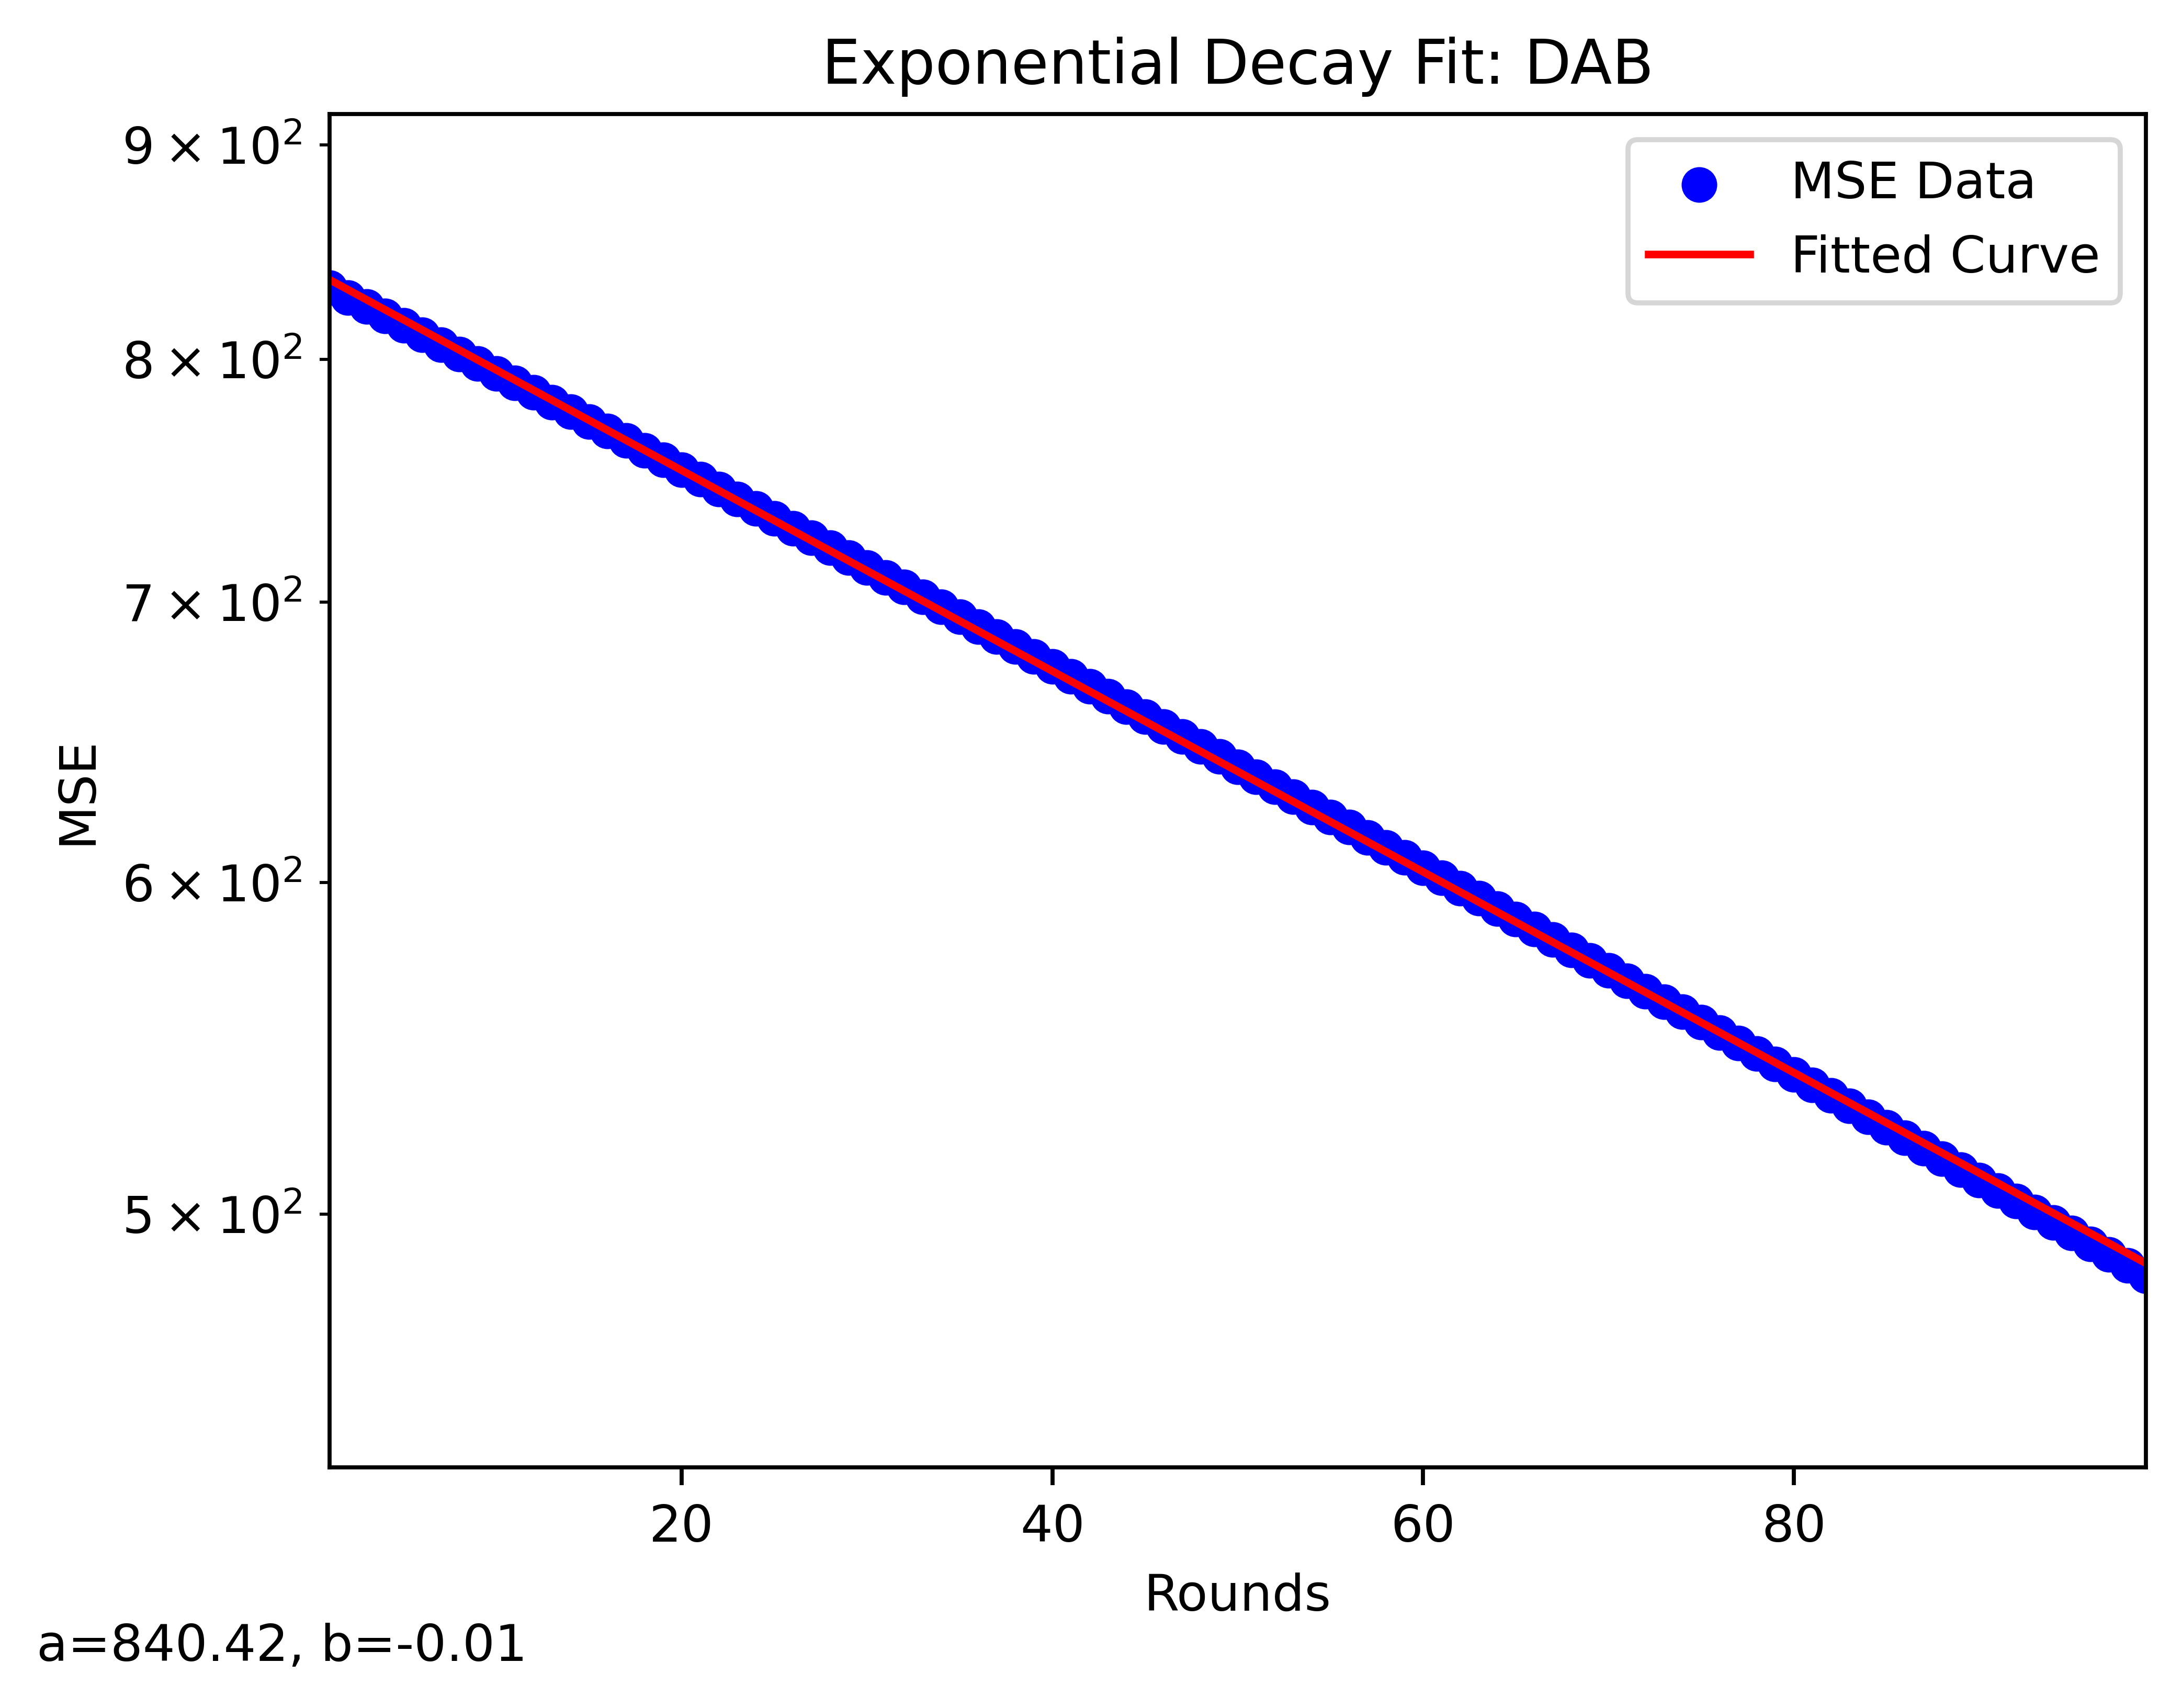
\includegraphics{figures/Simulation_outcomes/StarGraph/DAB/DAB_modelfitting_rounds_99_model_1.png}}
    \caption{Star graph - exponential regression fit: DAB}
    \label{fig:dabStarModelFit}
\end{figure}
\begin{figure}[]
    \centering
    \scalebox{0.8}{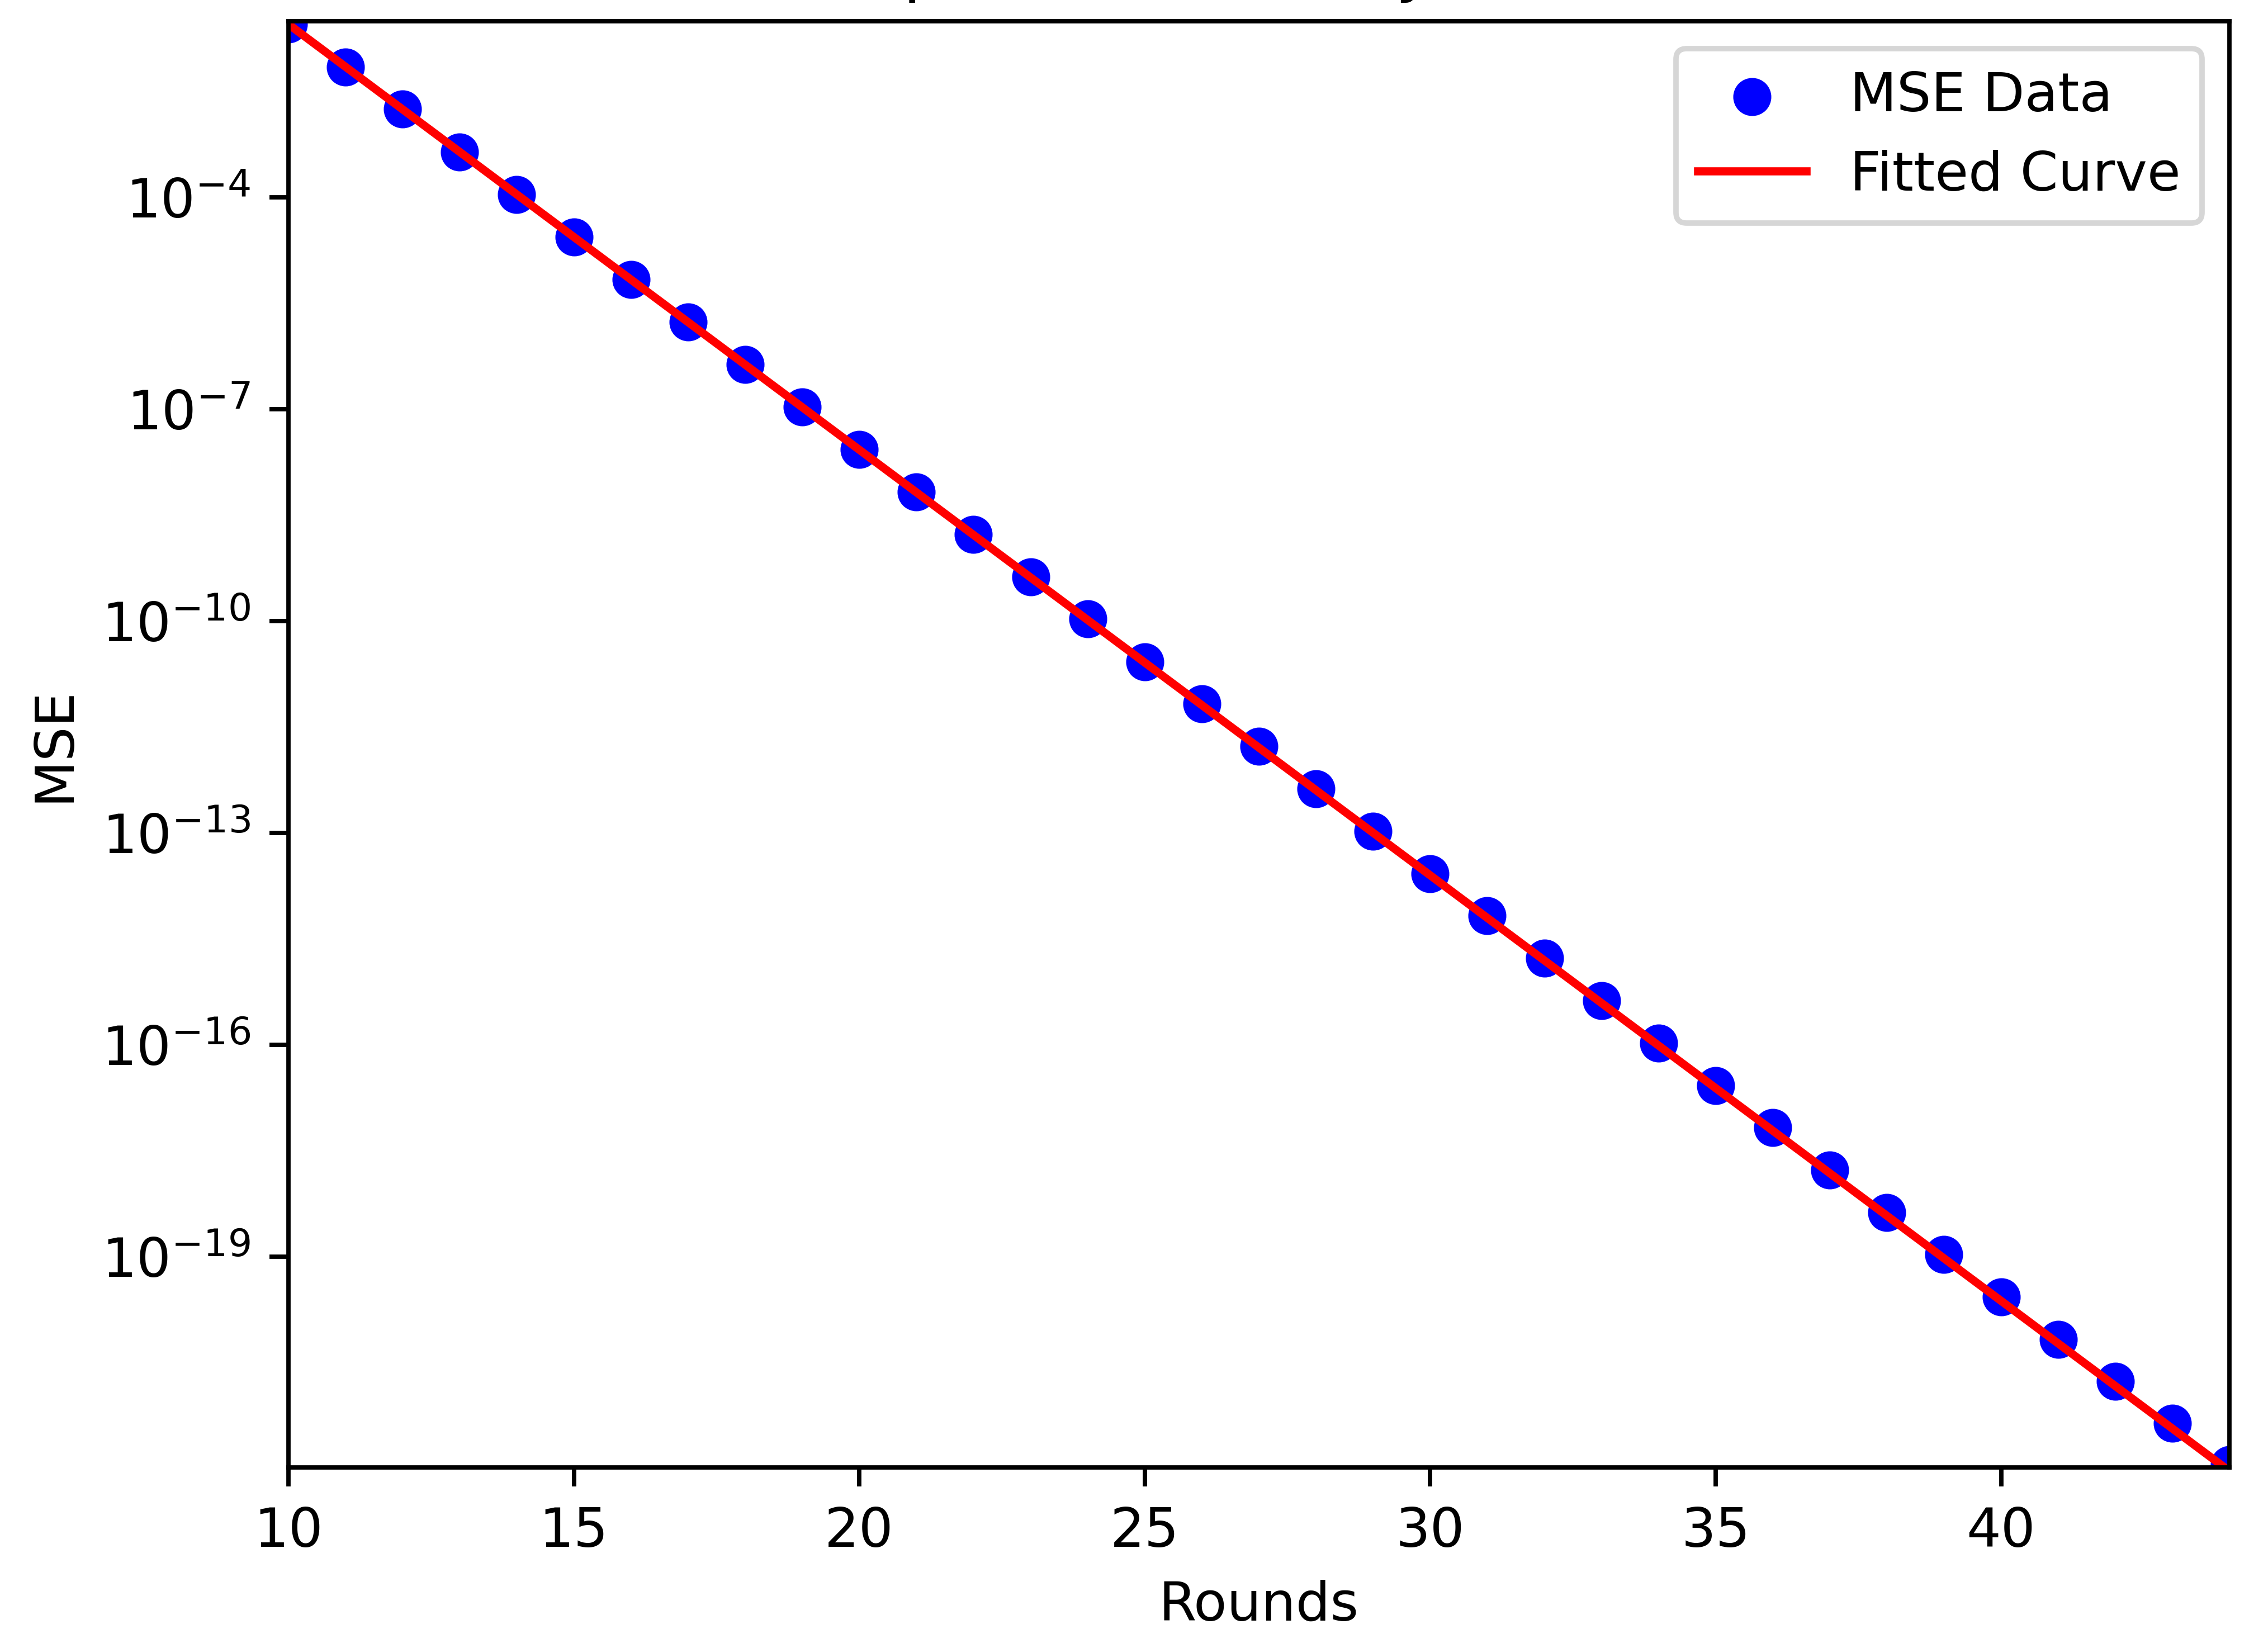
\includegraphics{figures/Simulation_outcomes/StarGraph/PPS/PPS_modelfitting_rounds_44_model_1.png}}
    \caption{Star graph - exponential regression fit: PPS}
    \label{fig:ppsStarModelFit}
\end{figure}
\begin{figure}[]
    \centering
    \scalebox{0.8}{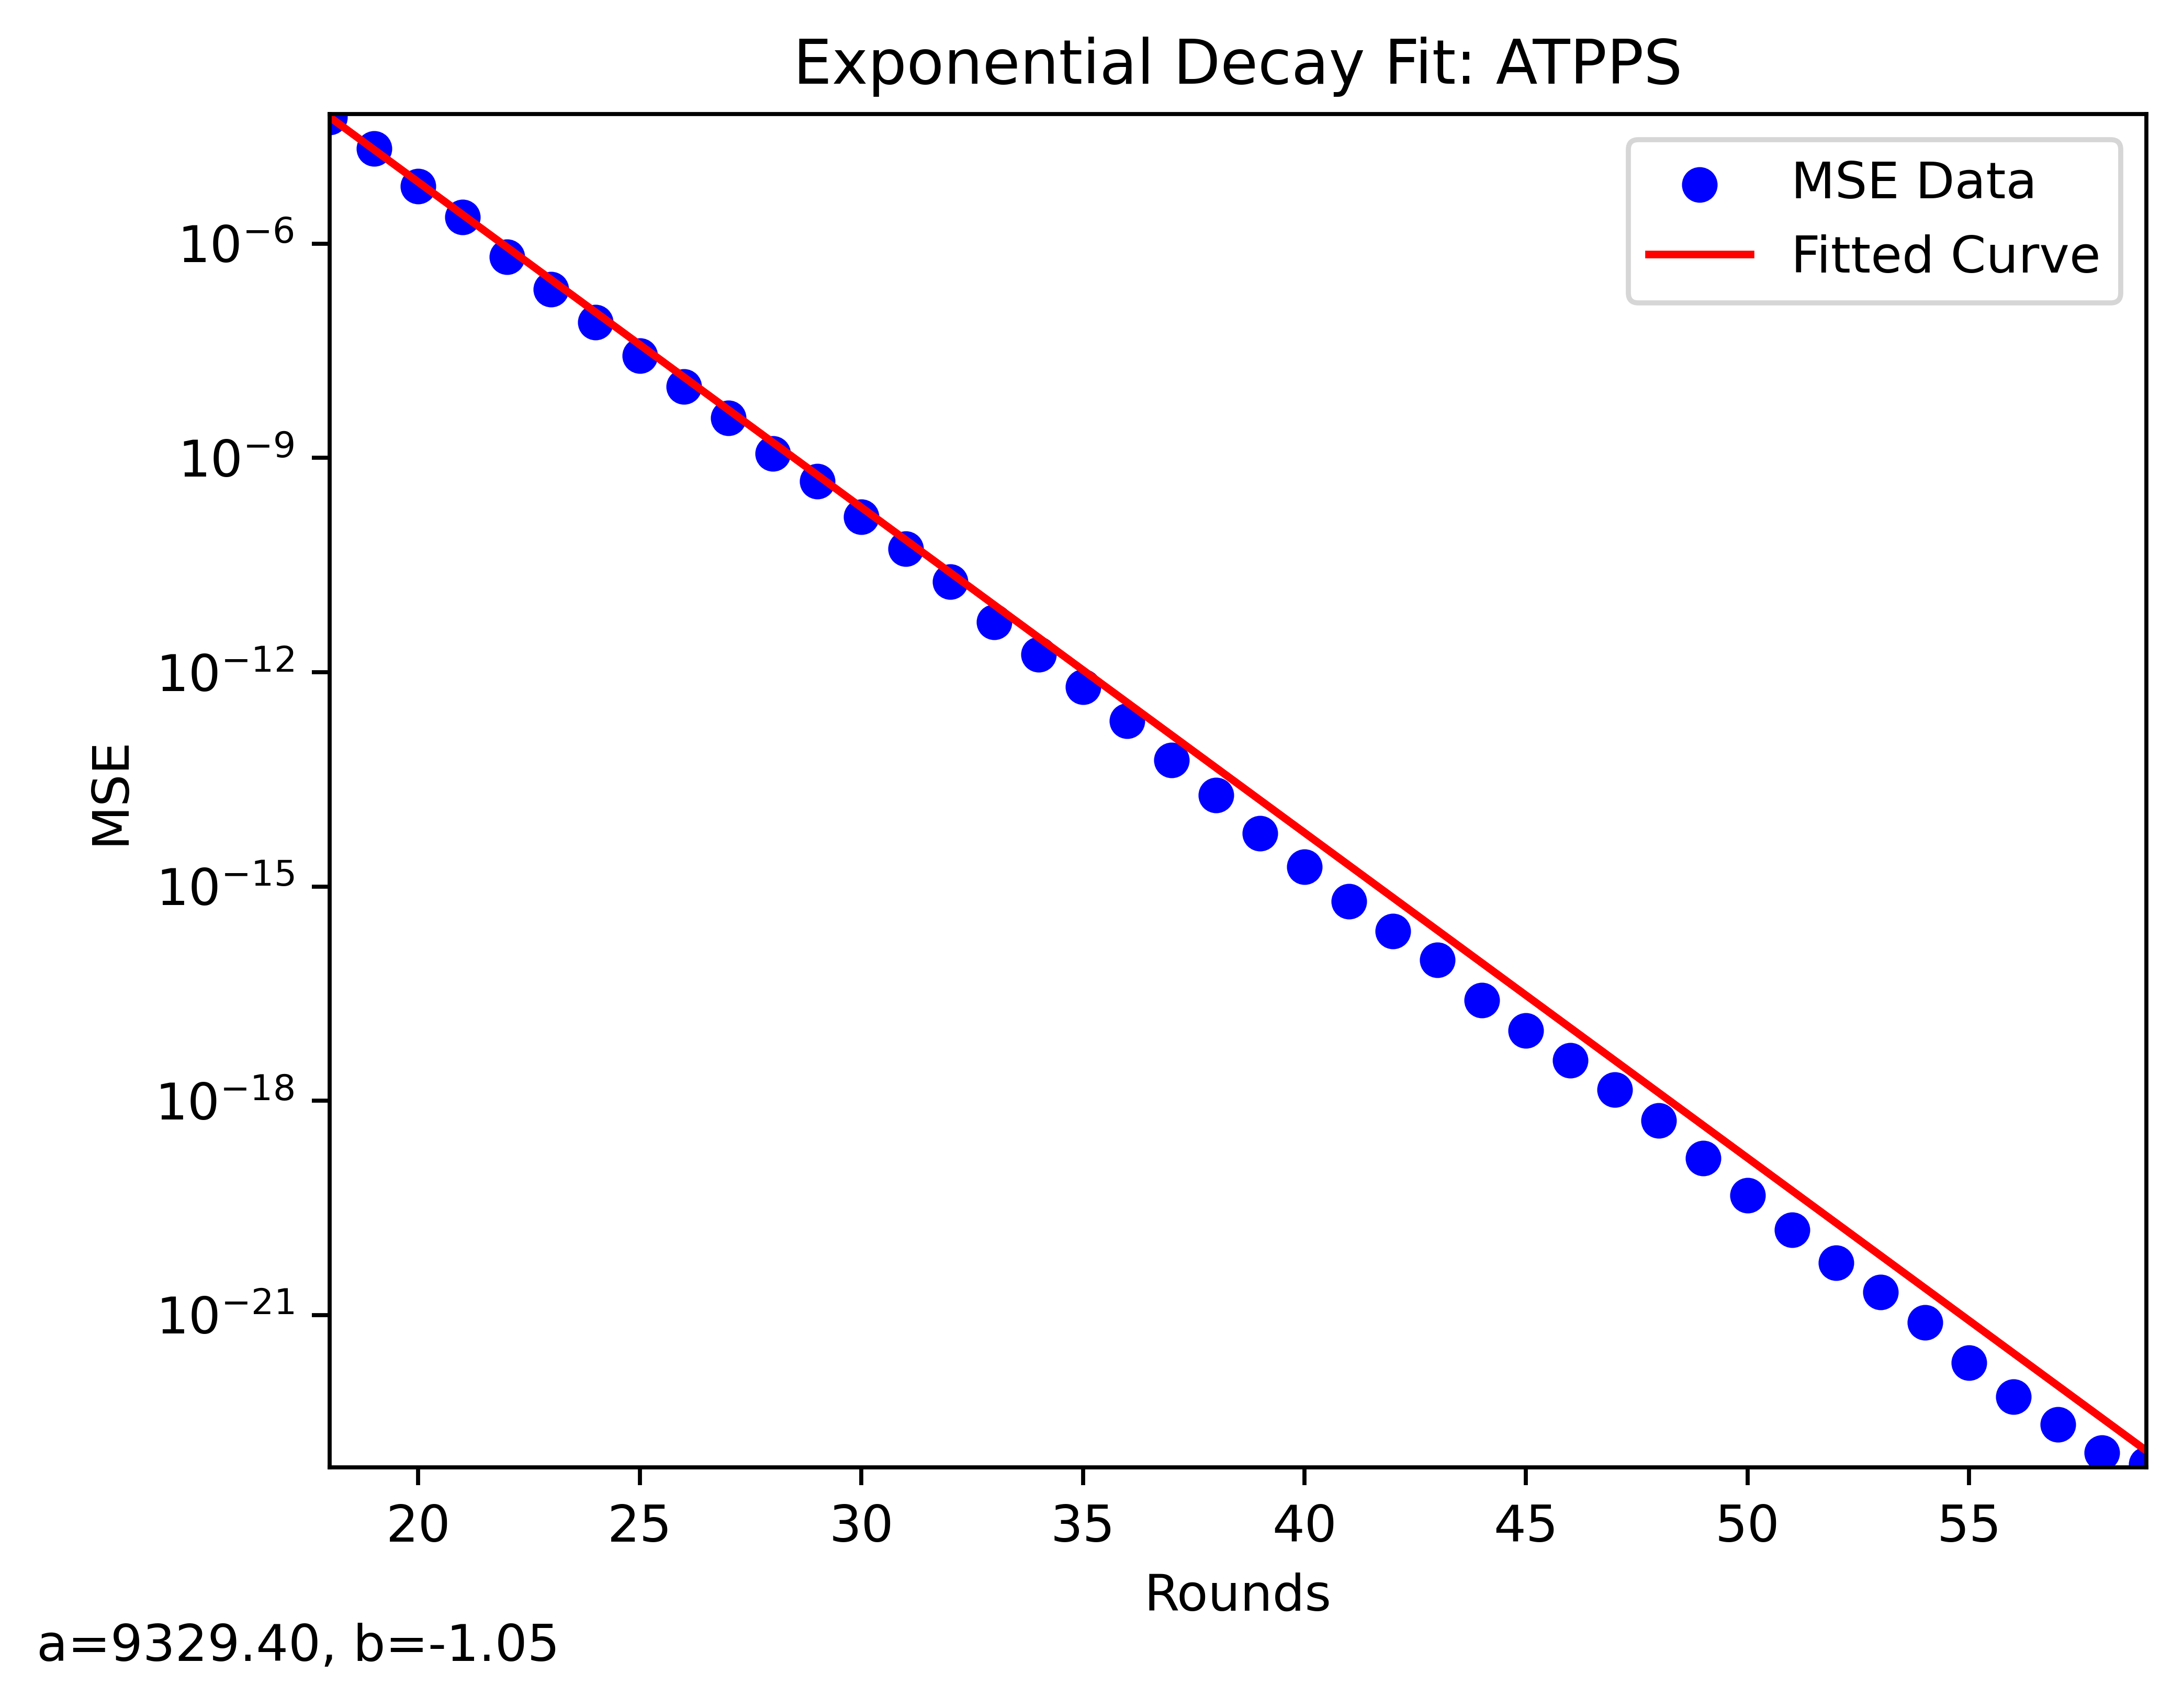
\includegraphics{figures/Simulation_outcomes/StarGraph/ATPPS/ATPPS_modelfitting_rounds_59_model_1.png}}
    \caption{Star graph - exponential regression fit: ATPPS}
    \label{fig:atppsStarModelFit}
\end{figure}
\begin{figure}
    \centering
    \scalebox{0.8}{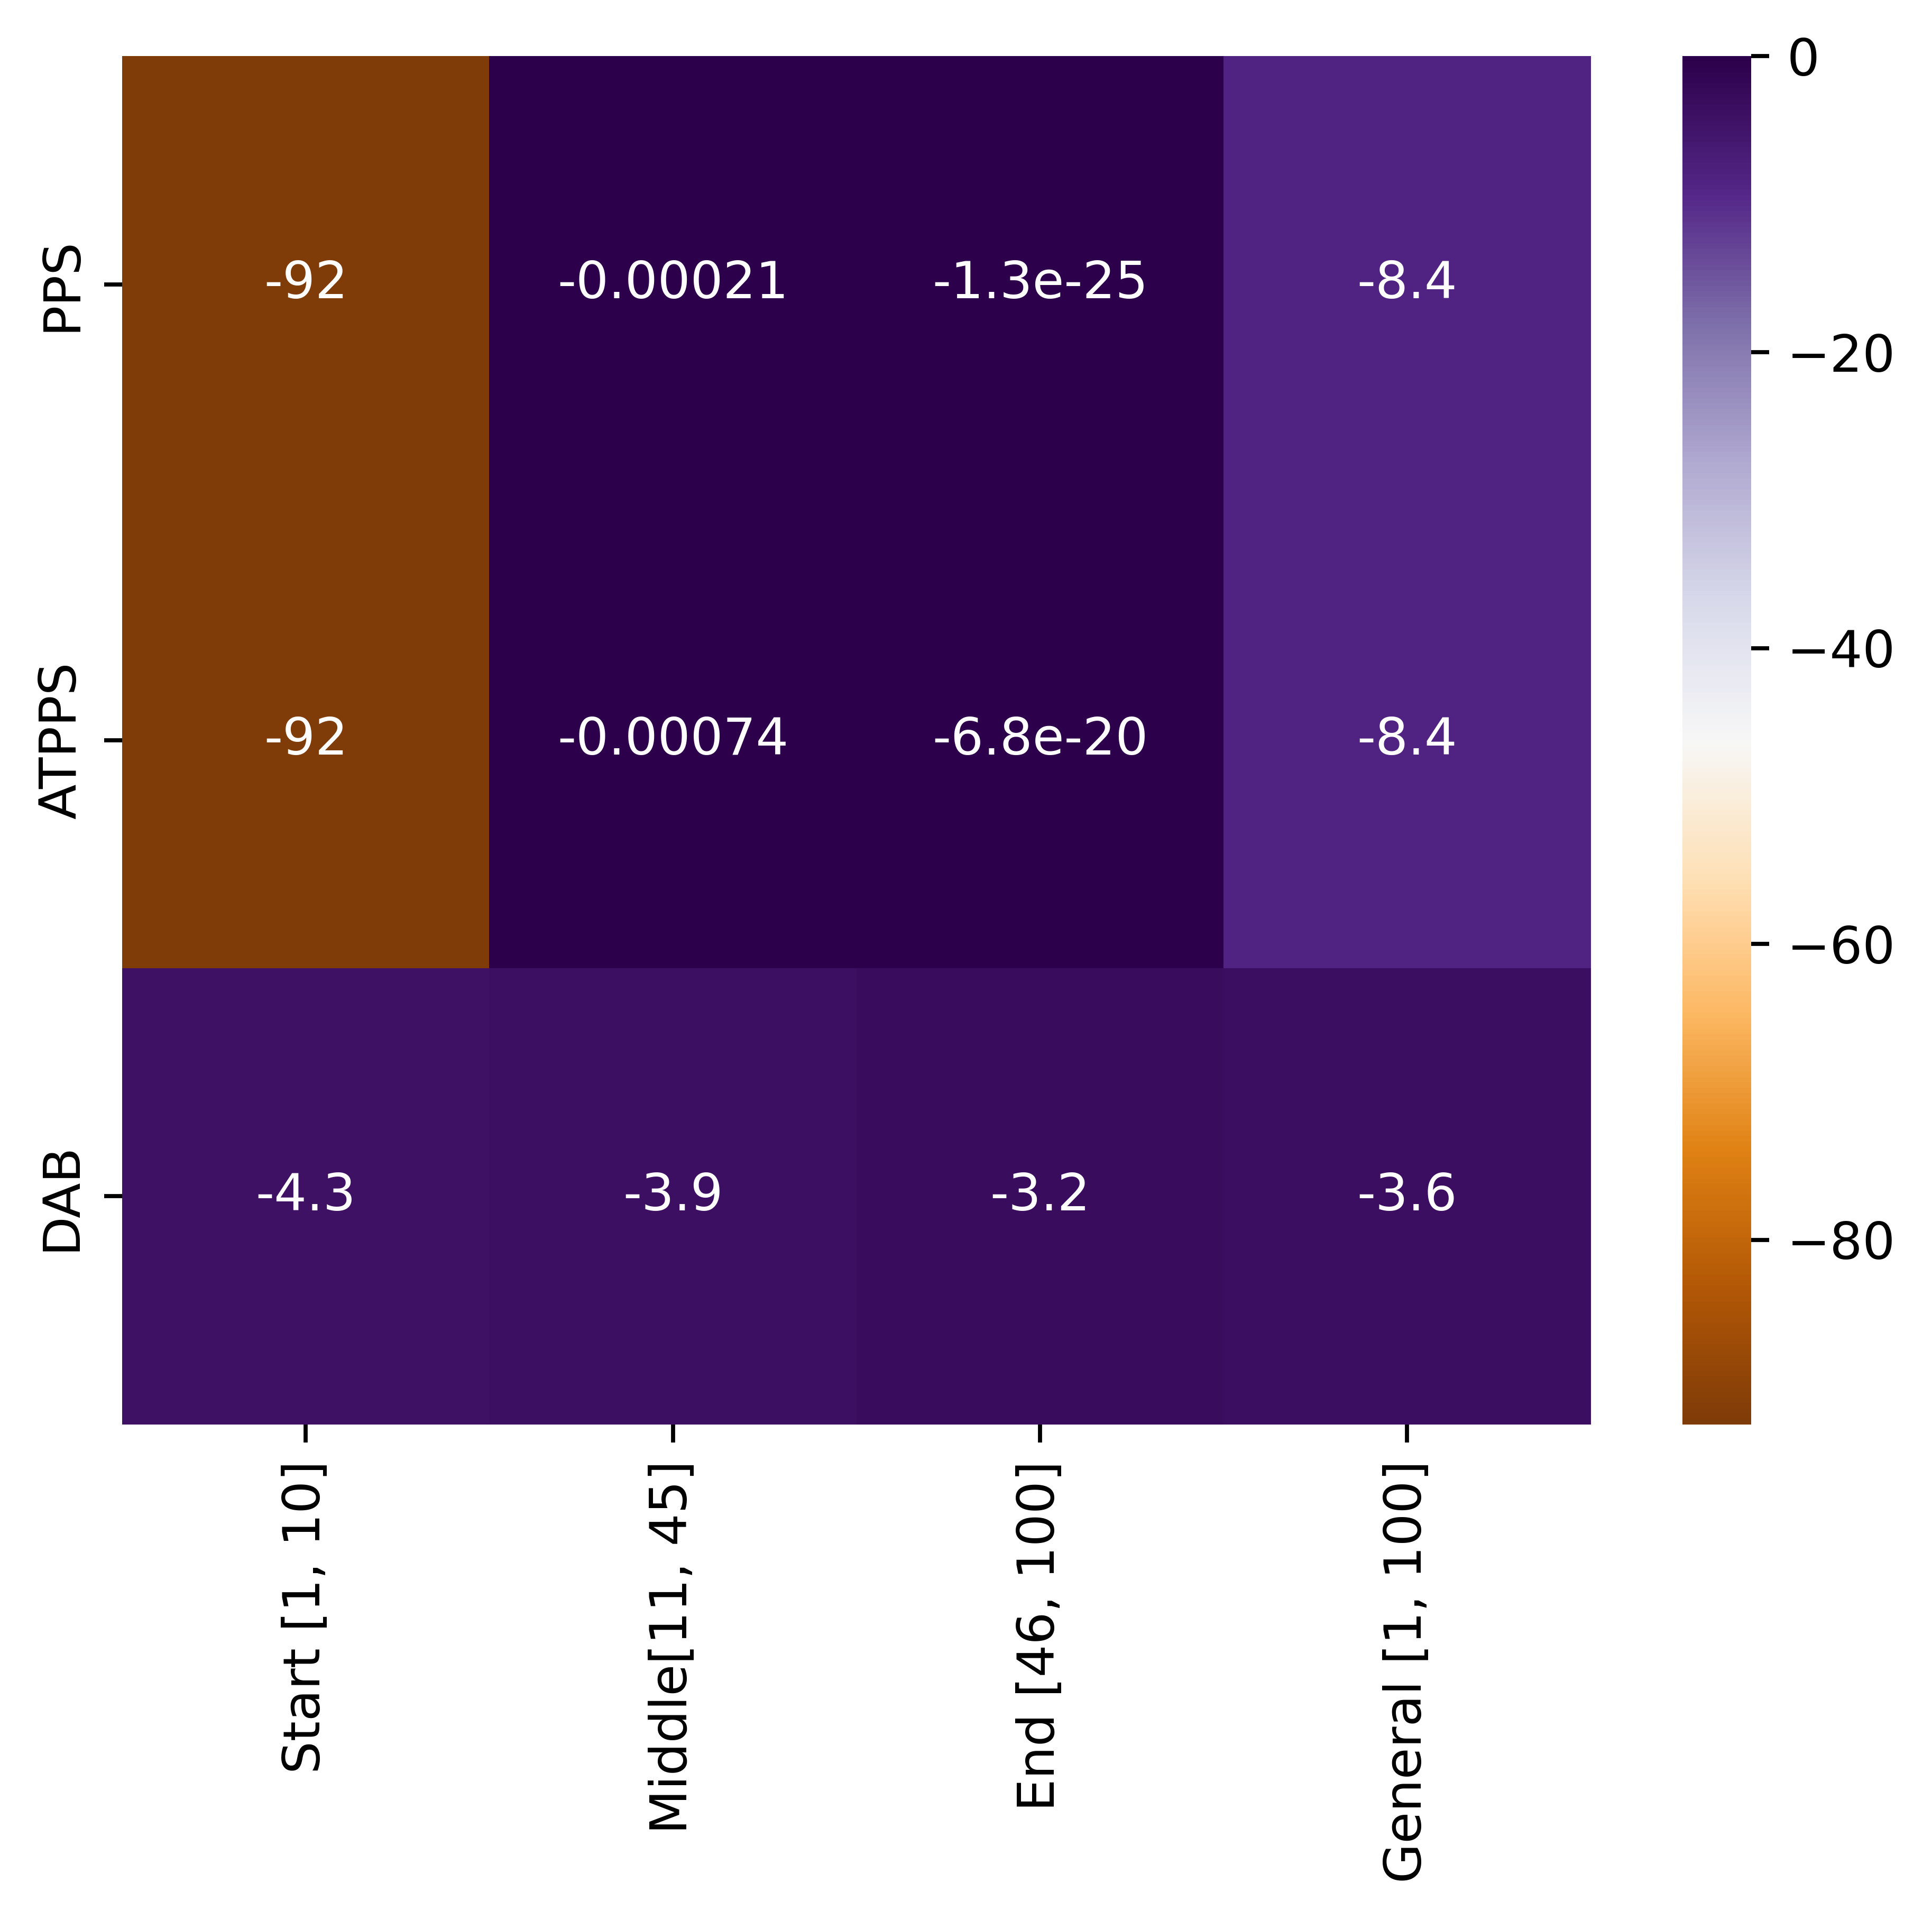
\includegraphics{figures/Simulation_outcomes/StarGraph/DAB_vs_PPS_vs_ATPPS_slopesheatmap_100rounds.png}}
    \caption{Star graph: heat map of slopes per region}
    \label{fig:stargraphslopes}
\end{figure}

\section{Ring Graph}\label{sec:ringgraph}
The DAB curve in figure \ref{fig:ringgraphMSEperRoundLogLog} shows the steepest decline in error in the first few rounds of the simulation. The slope of the first 10 rounds is -84 for the DAB curve compared to -82 for each Push-Pull Sum based algorithm as depicted in figure \ref{fig:ringgraphslopes}. The near-overlap of PPS and ATPPS across the 100 rounds of simulation indicates that the adaptive mechanism provides limited additional benefit in a Ring graph, where choosing a random neighbor might already target the optimal load transfer partner. In the sense that in a Ring topology, each node only has access to its two neighbors. The adaptive threshold mechanism relies on meaningful differences in load between nodes to trigger exchanges, but in a Ring graph, local differences might not vary significantly enough to make the threshold mechanism advantageous for each neighborhood. For the PPS, every node communicates with its neighbors in every round. This constant exchange ensures rapid propagation of load updates. The adaptive threshold might reduce some of these exchanges, but in a Ring graph, where the diameter is large, reducing communication might delay convergence rather than improve it. Thus, the threshold mechanism could counteract its own benefits, limiting the advantage of the ATPPS over the PPS. The DAB functions way better in this scenario, since it always interacts with the optimal partner to exchange loads. The randomness benefit vanishes for a network topology where each node only has two neighbors, and a deterministic approach actually performs better.

The MSE data of each algorithms simulations were fitted to the polynomial regression model with degree of 4 each. The best-fit model for the DAB MSE data for the rounds 10 to 60 follow the equation: $MSE_r=1.72\times 10^{-5}r^{4}-2.30\times 10^{-3}r^{3}+ 0.19r^{2}-5.99r+114.83$ (figure \ref{fig:dabRingModelFit}). A similiar equation is fitted for the PPS and ATPPS curves: $MSE_r= 2.99\times 10^{-5}r^{4}-0.5\times 10^{-2}r^{3} + 0.32r^{2} -9.68r + 166.30$ (figure \ref{fig:ppsRingModelFit}) for the PPS, and for the ATPPS: $MSE_r=3.04\times 10^{-5}r^{4}-0.5\times 10^{-2}r^{3} + 0.32r^{2}-9.64r+161.86$ (figure \ref{fig:atppsRingModelFit}).

\begin{figure}[]
    \centering
    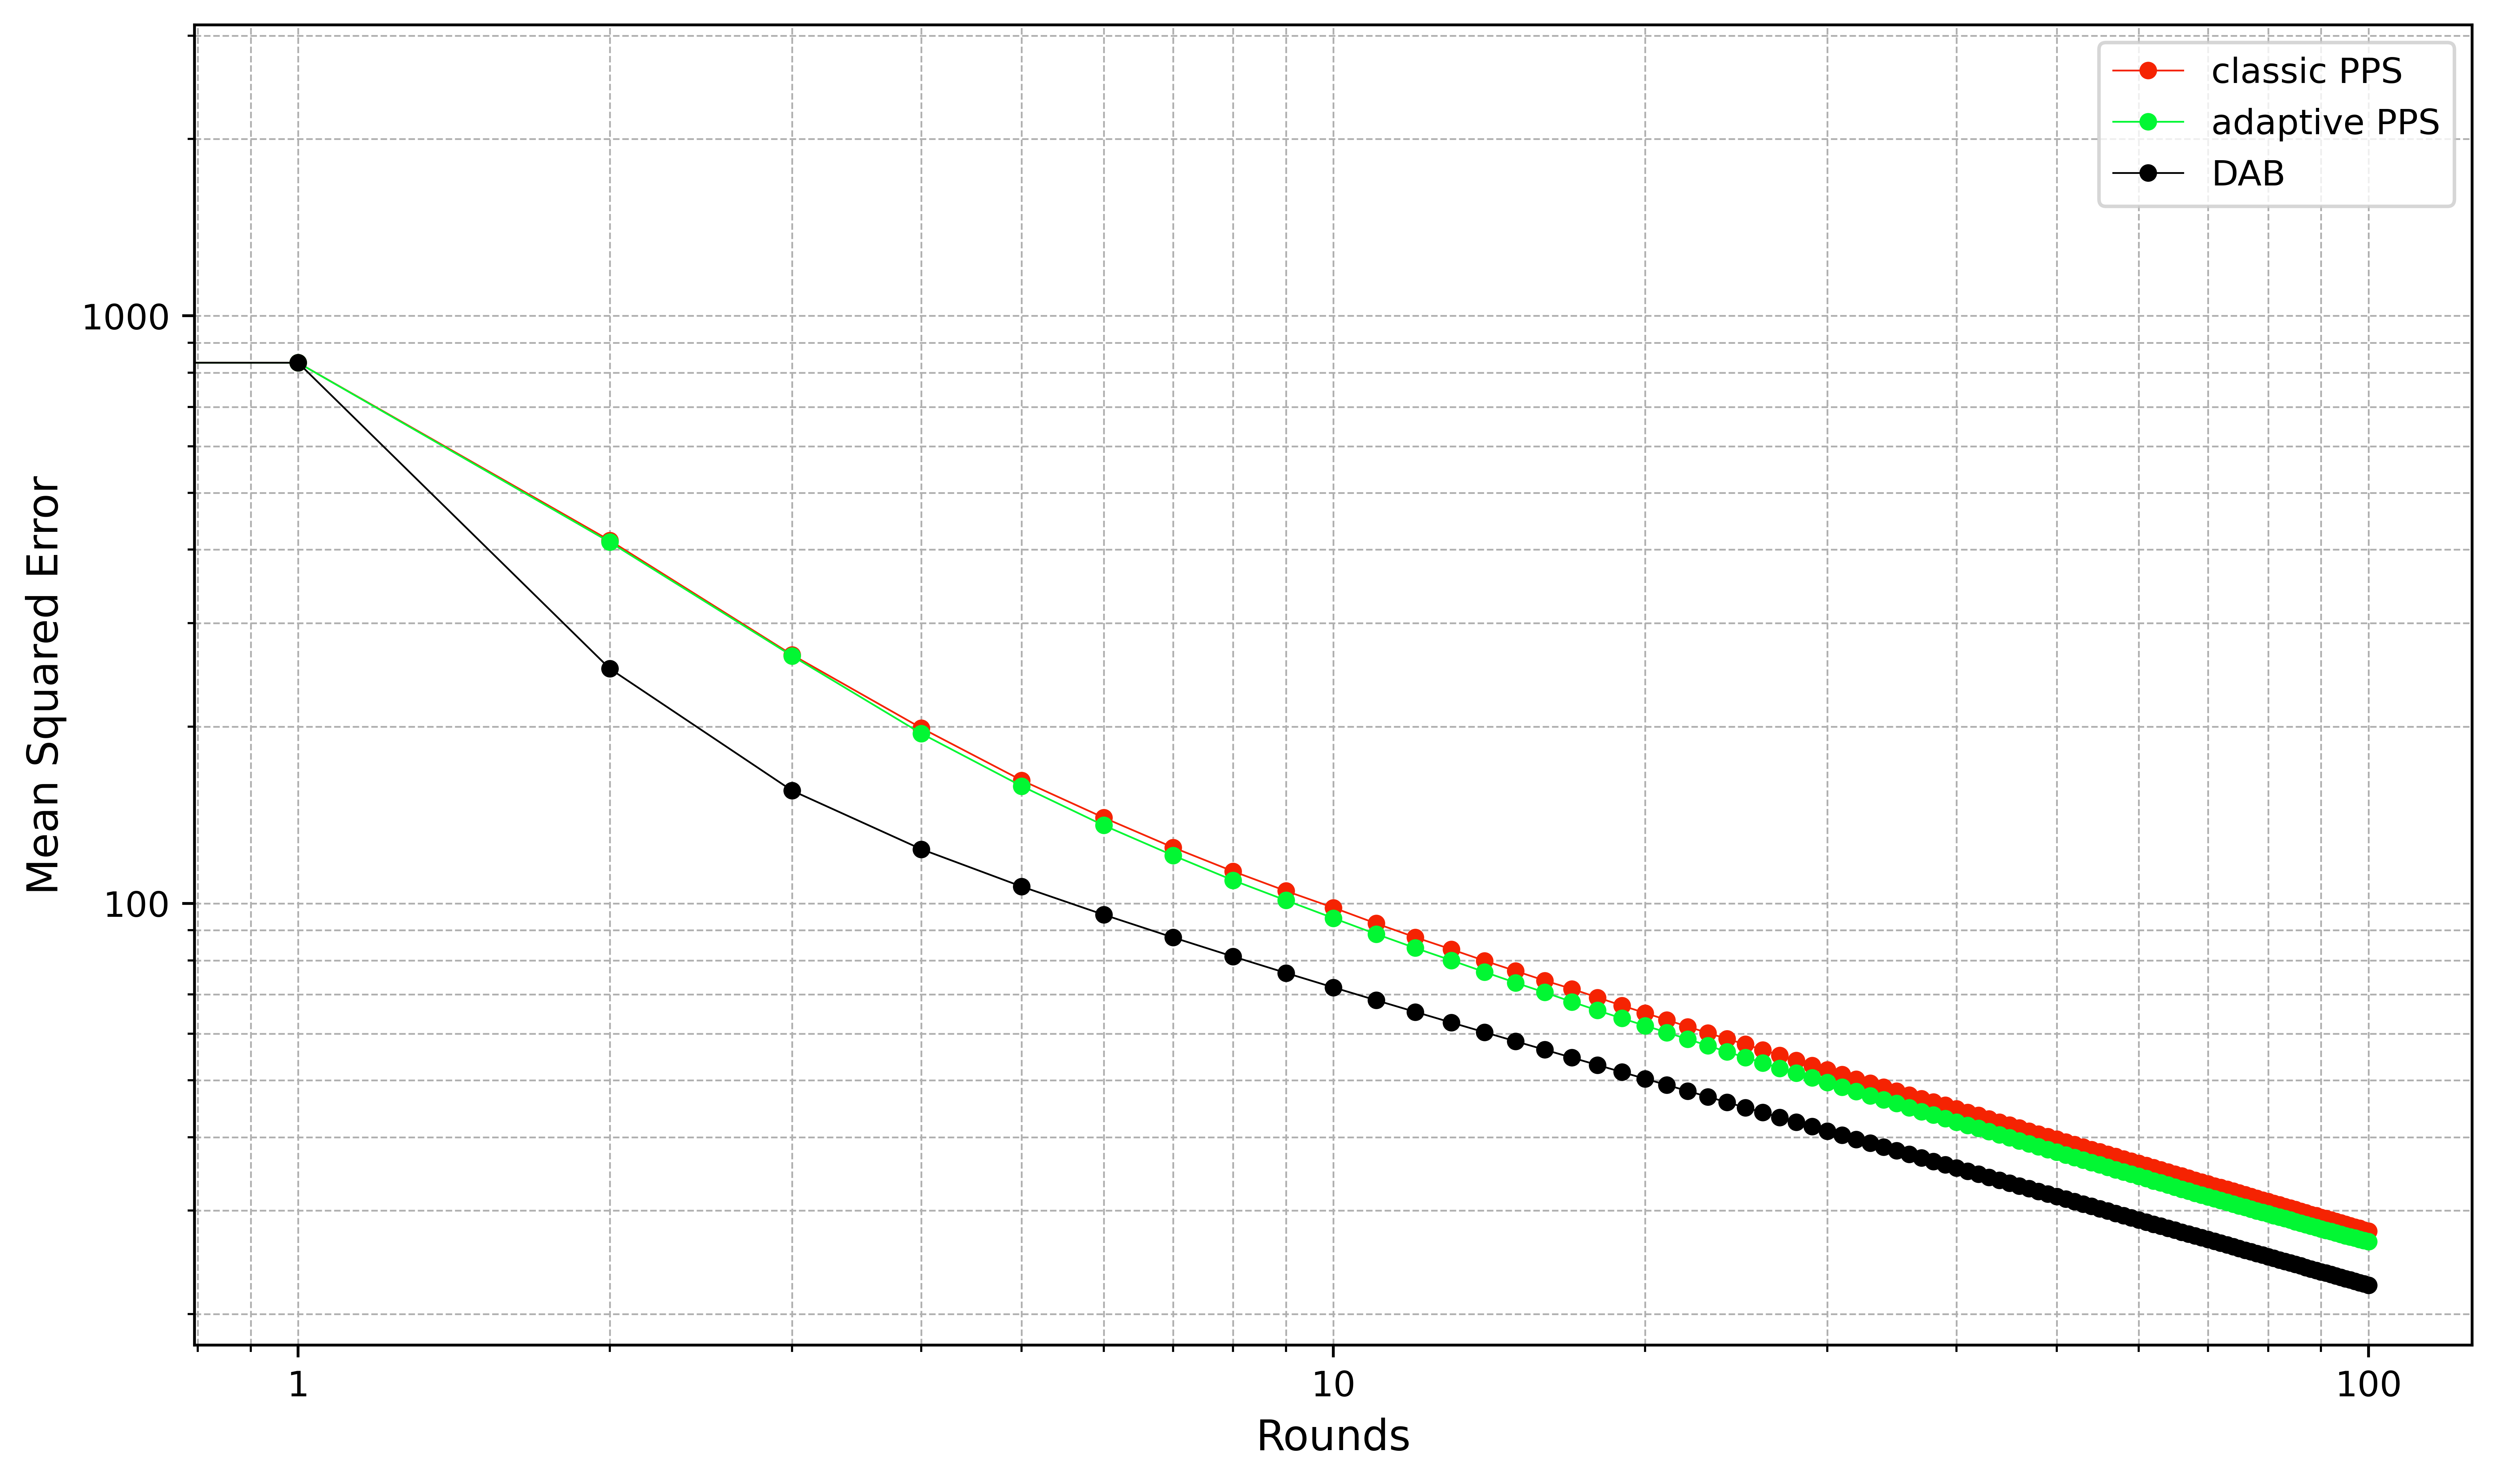
\includegraphics[width=\linewidth]{figures/Simulation_outcomes/RingGraph/DAB_vs_PPS_RG_r100_n1024_averaged_loglog.png}
    \caption{Ring graph: mean squared error per rounds (log-log)}
    \label{fig:ringgraphMSEperRoundLogLog}
\end{figure}
\begin{figure}[]
    \centering
    \scalebox{0.8}{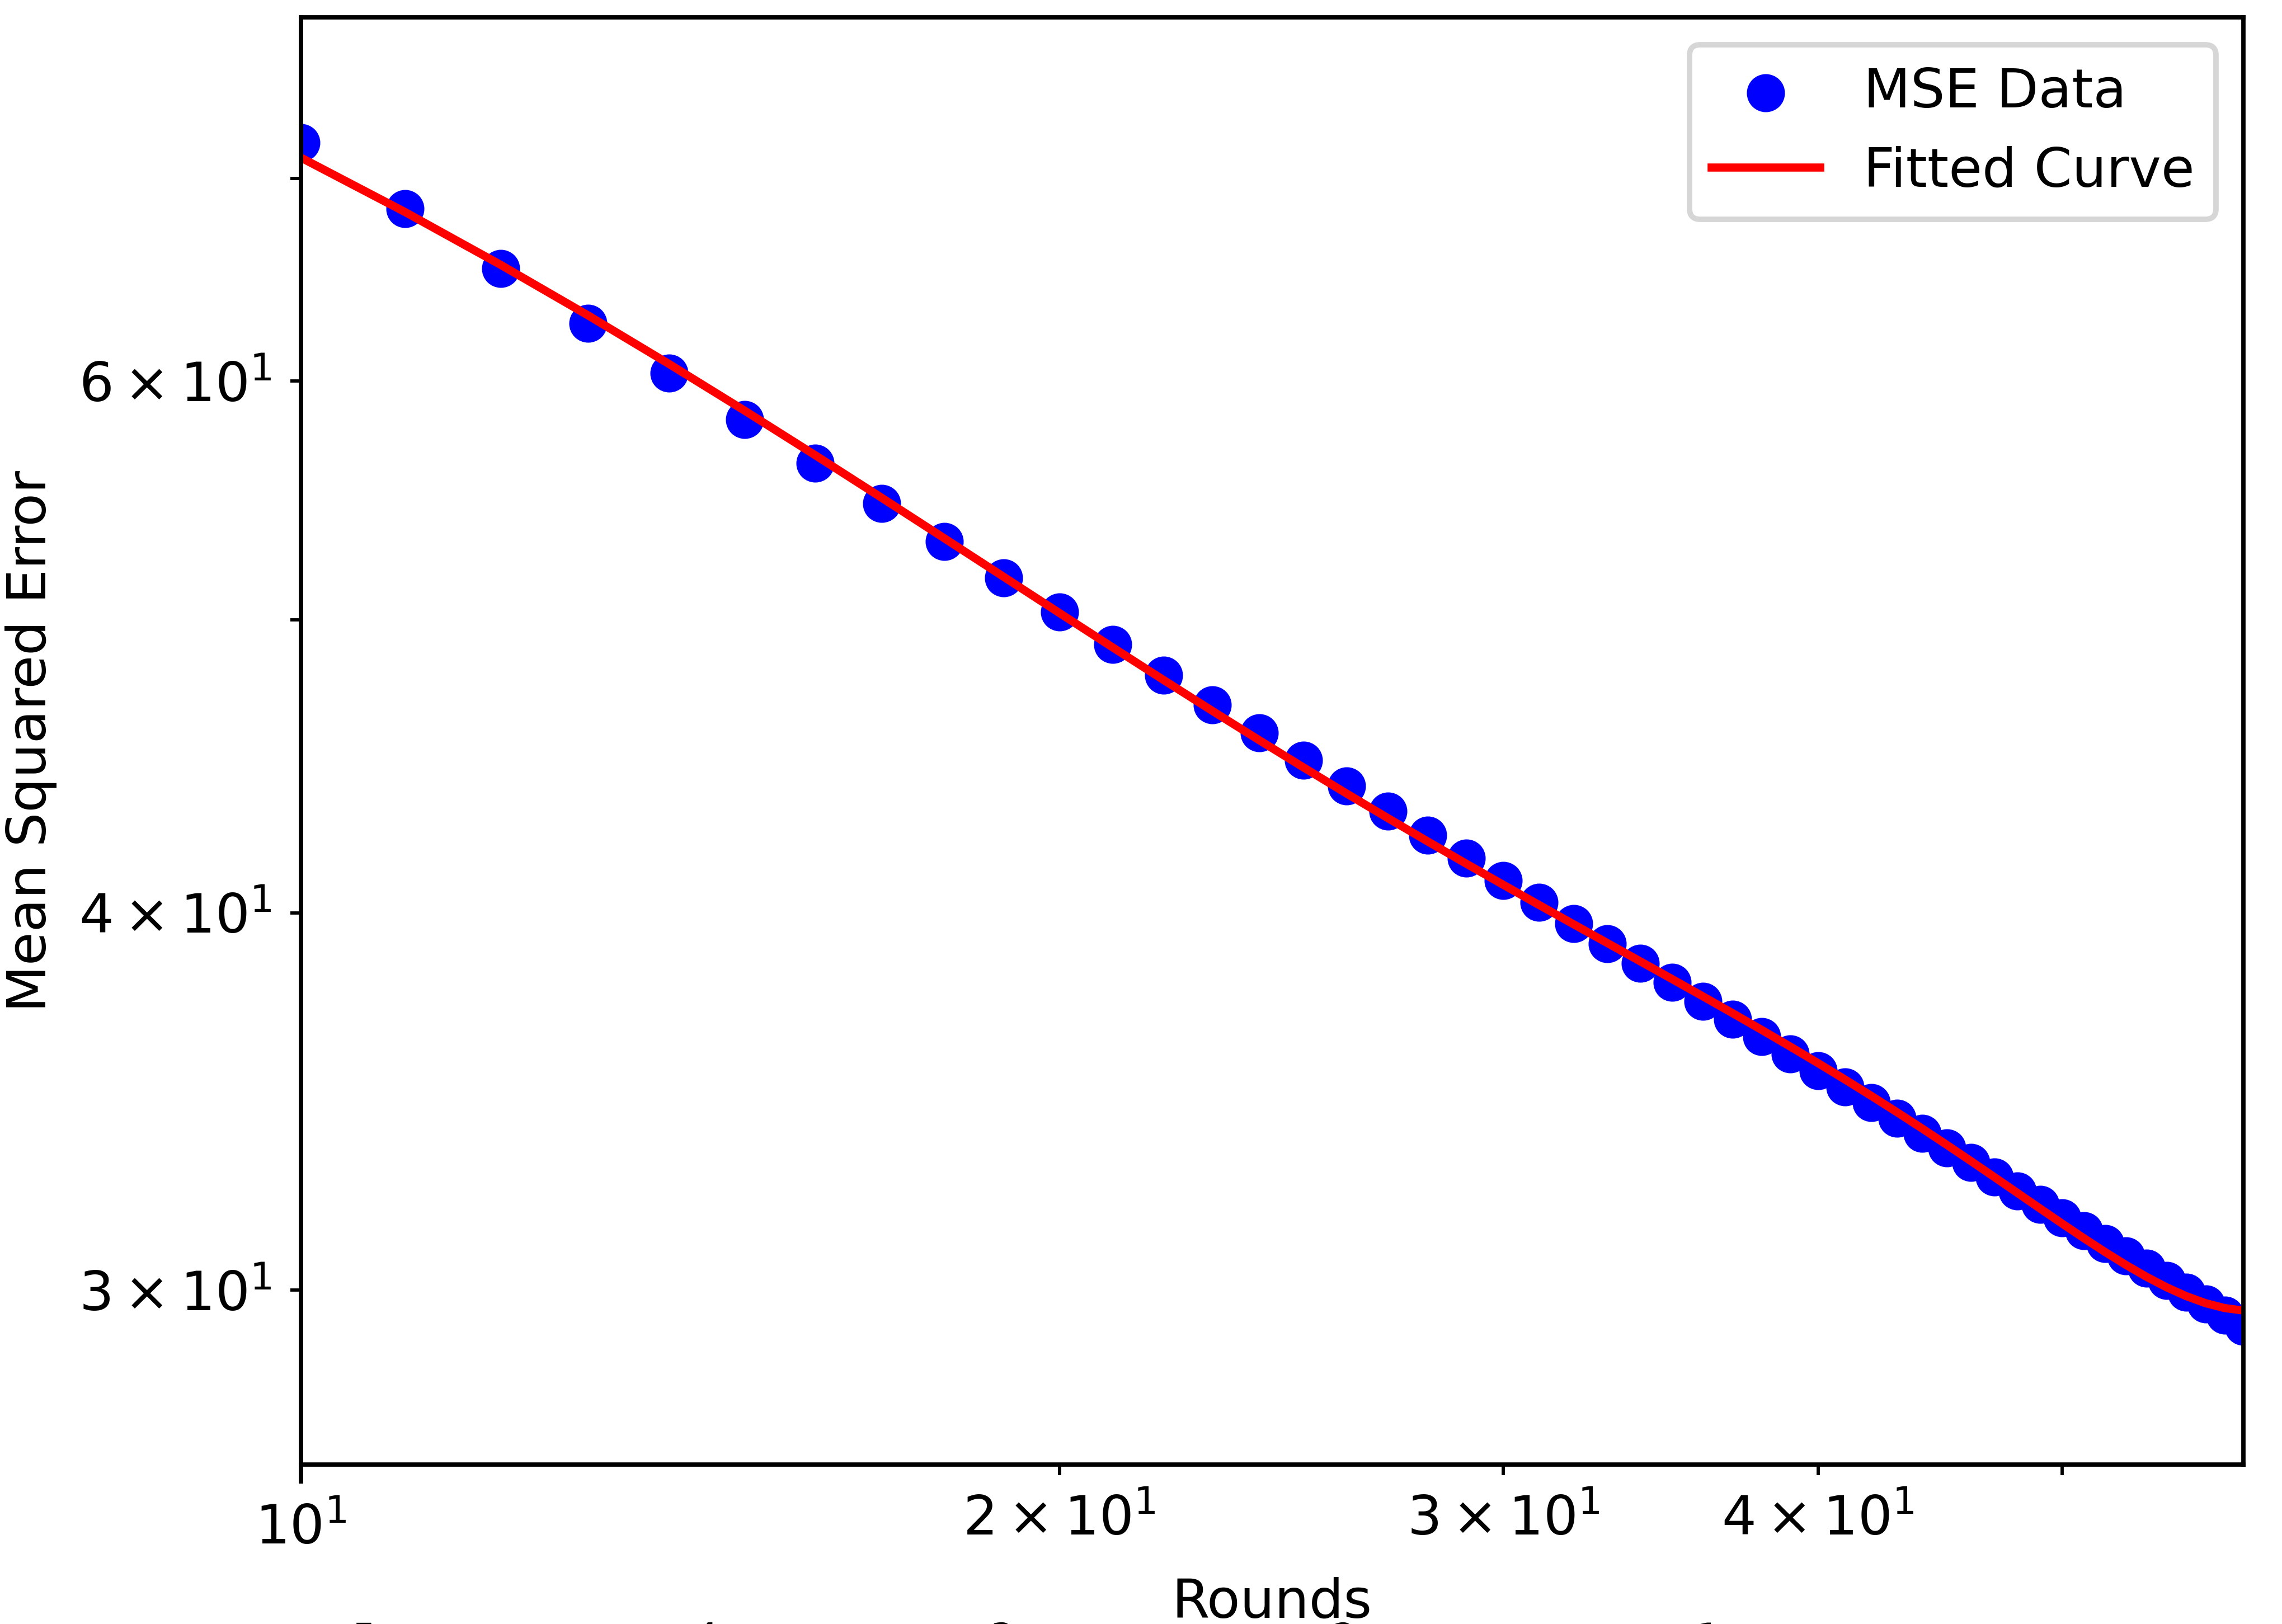
\includegraphics{figures/Simulation_outcomes/RingGraph/DAB/DAB_modelfitting_rounds_59_model_2.png}}
    \caption{Ring graph - polynomial regression fit: DAB}
    \label{fig:dabRingModelFit}
\end{figure}
\begin{figure}[]
   \centering
   \scalebox{0.8}{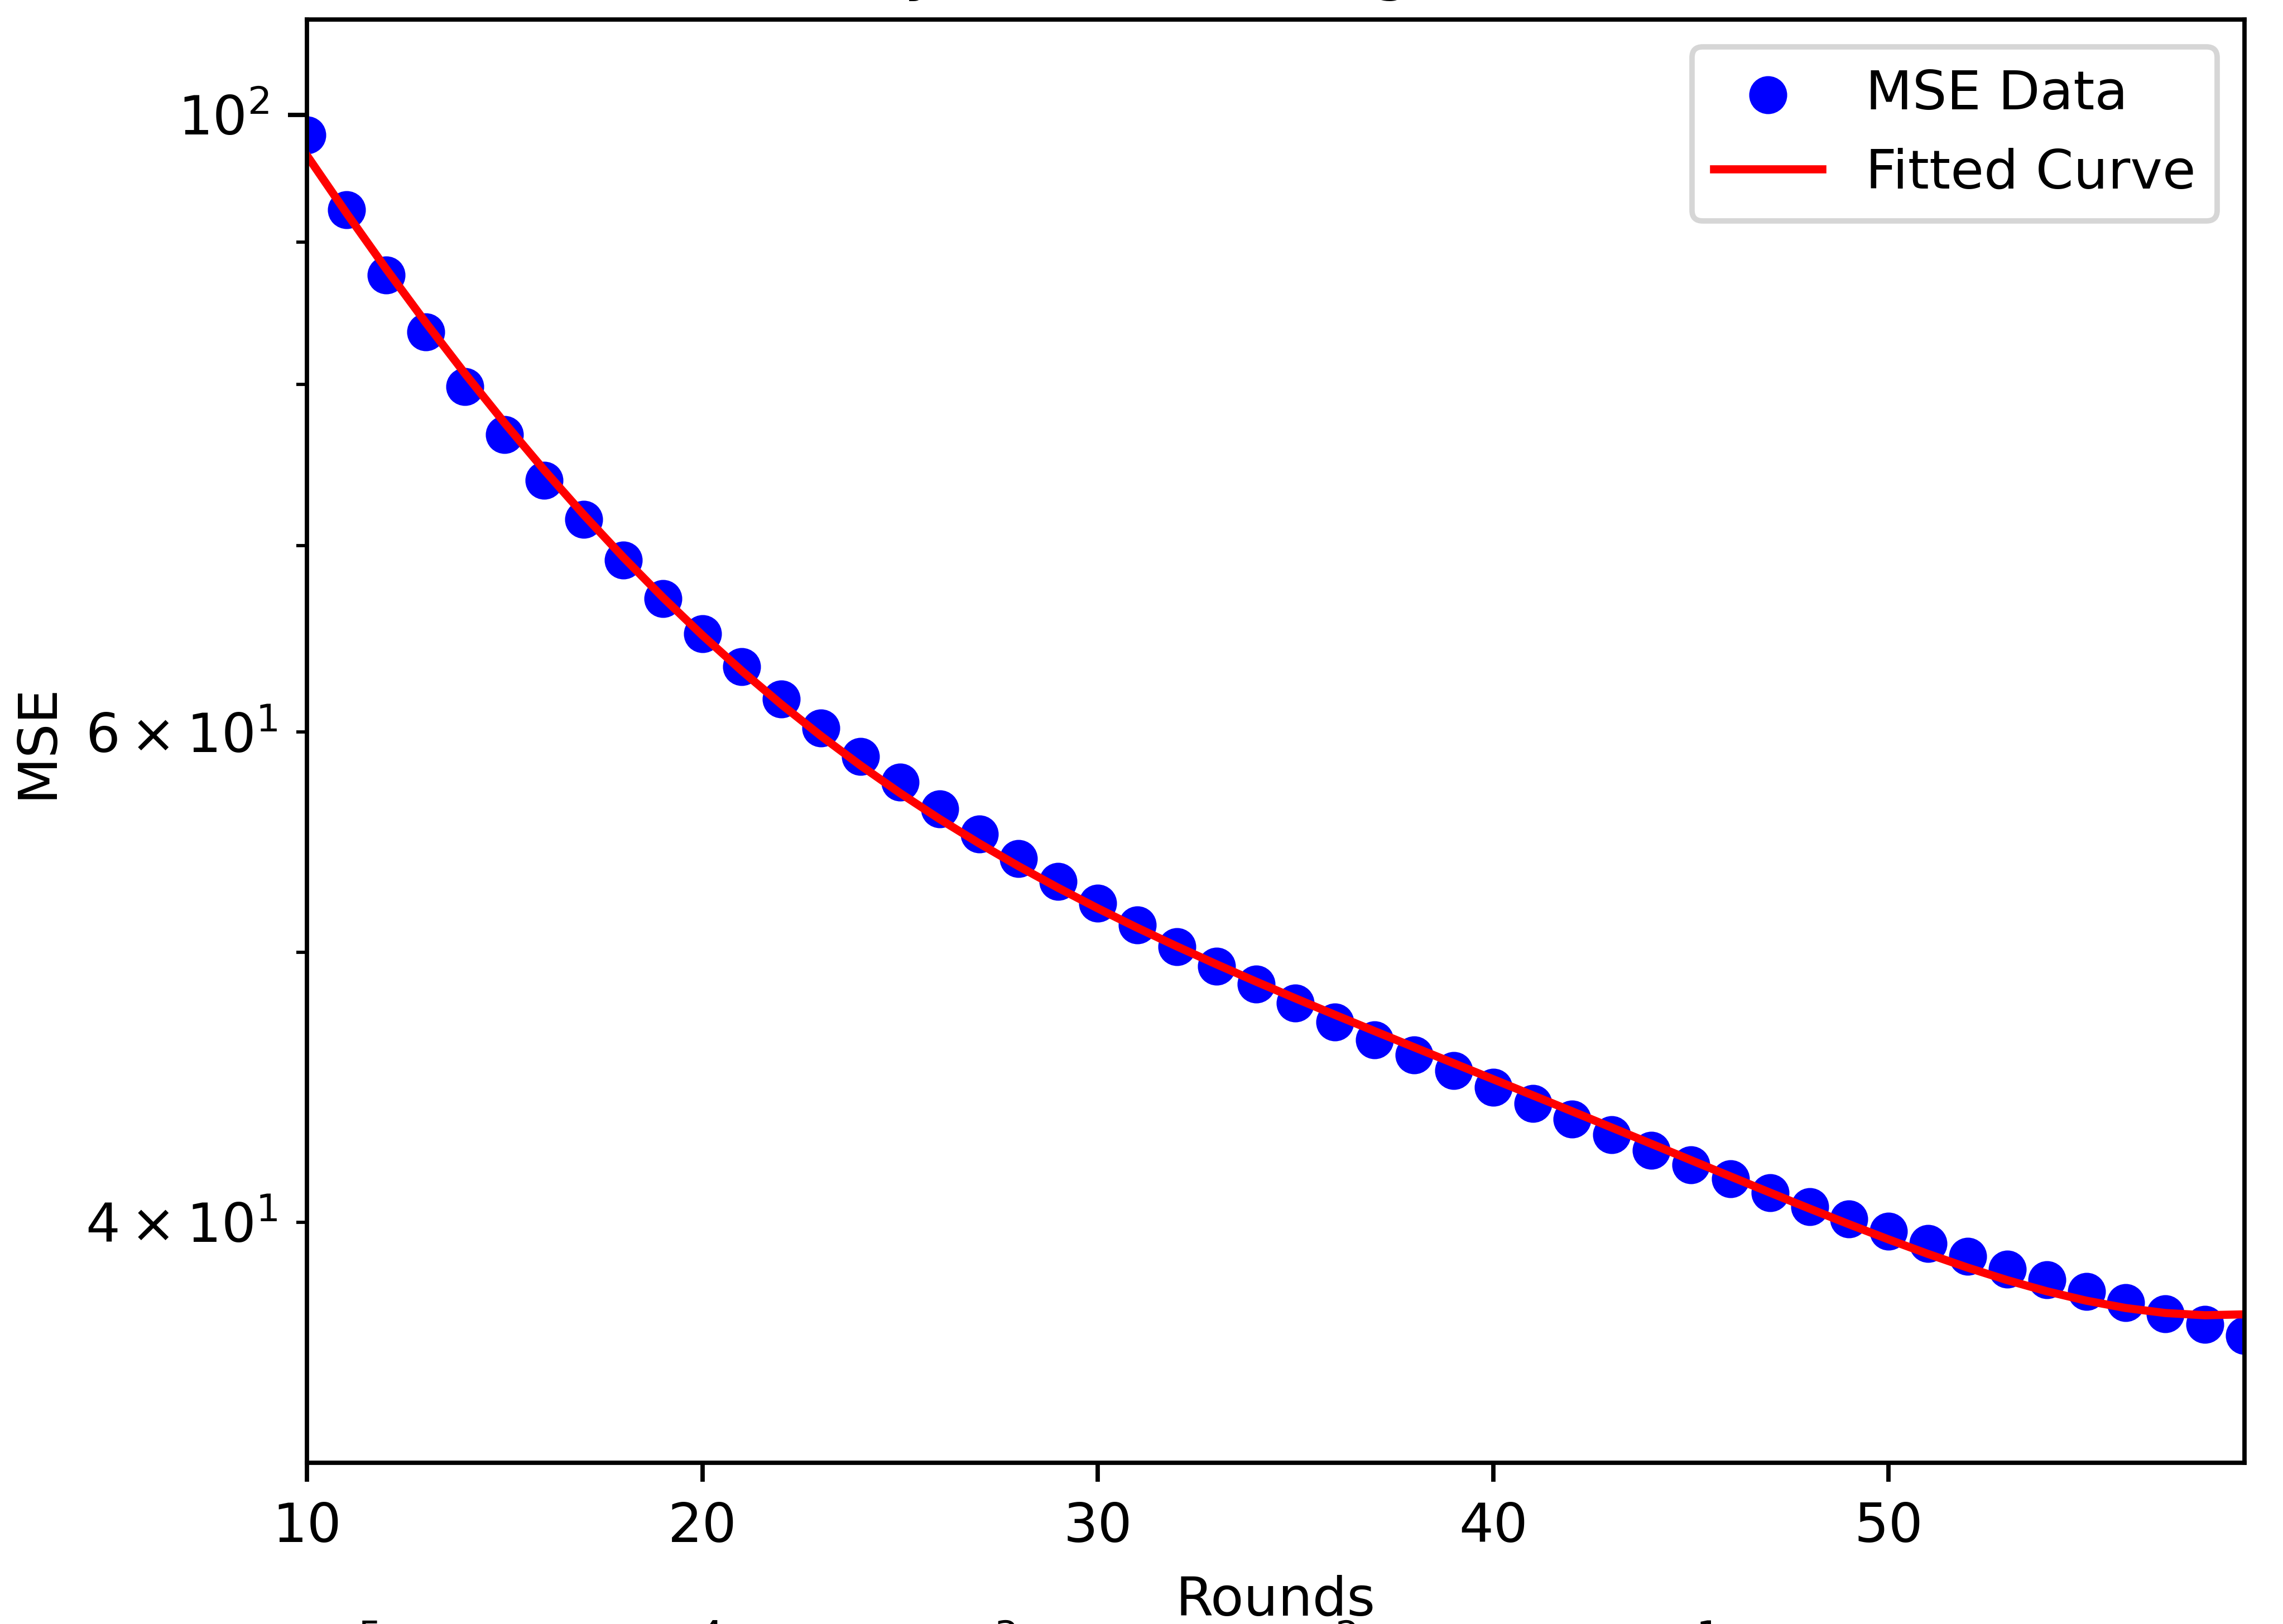
\includegraphics{figures/Simulation_outcomes/RingGraph/PPS/PPS_modelfitting_rounds_59_model_2.png}}
   \caption{Ring graph - polynomial regression fit: PPS}
   \label{fig:ppsRingModelFit}
\end{figure}
\begin{figure}[]
    \centering
    \scalebox{0.8}{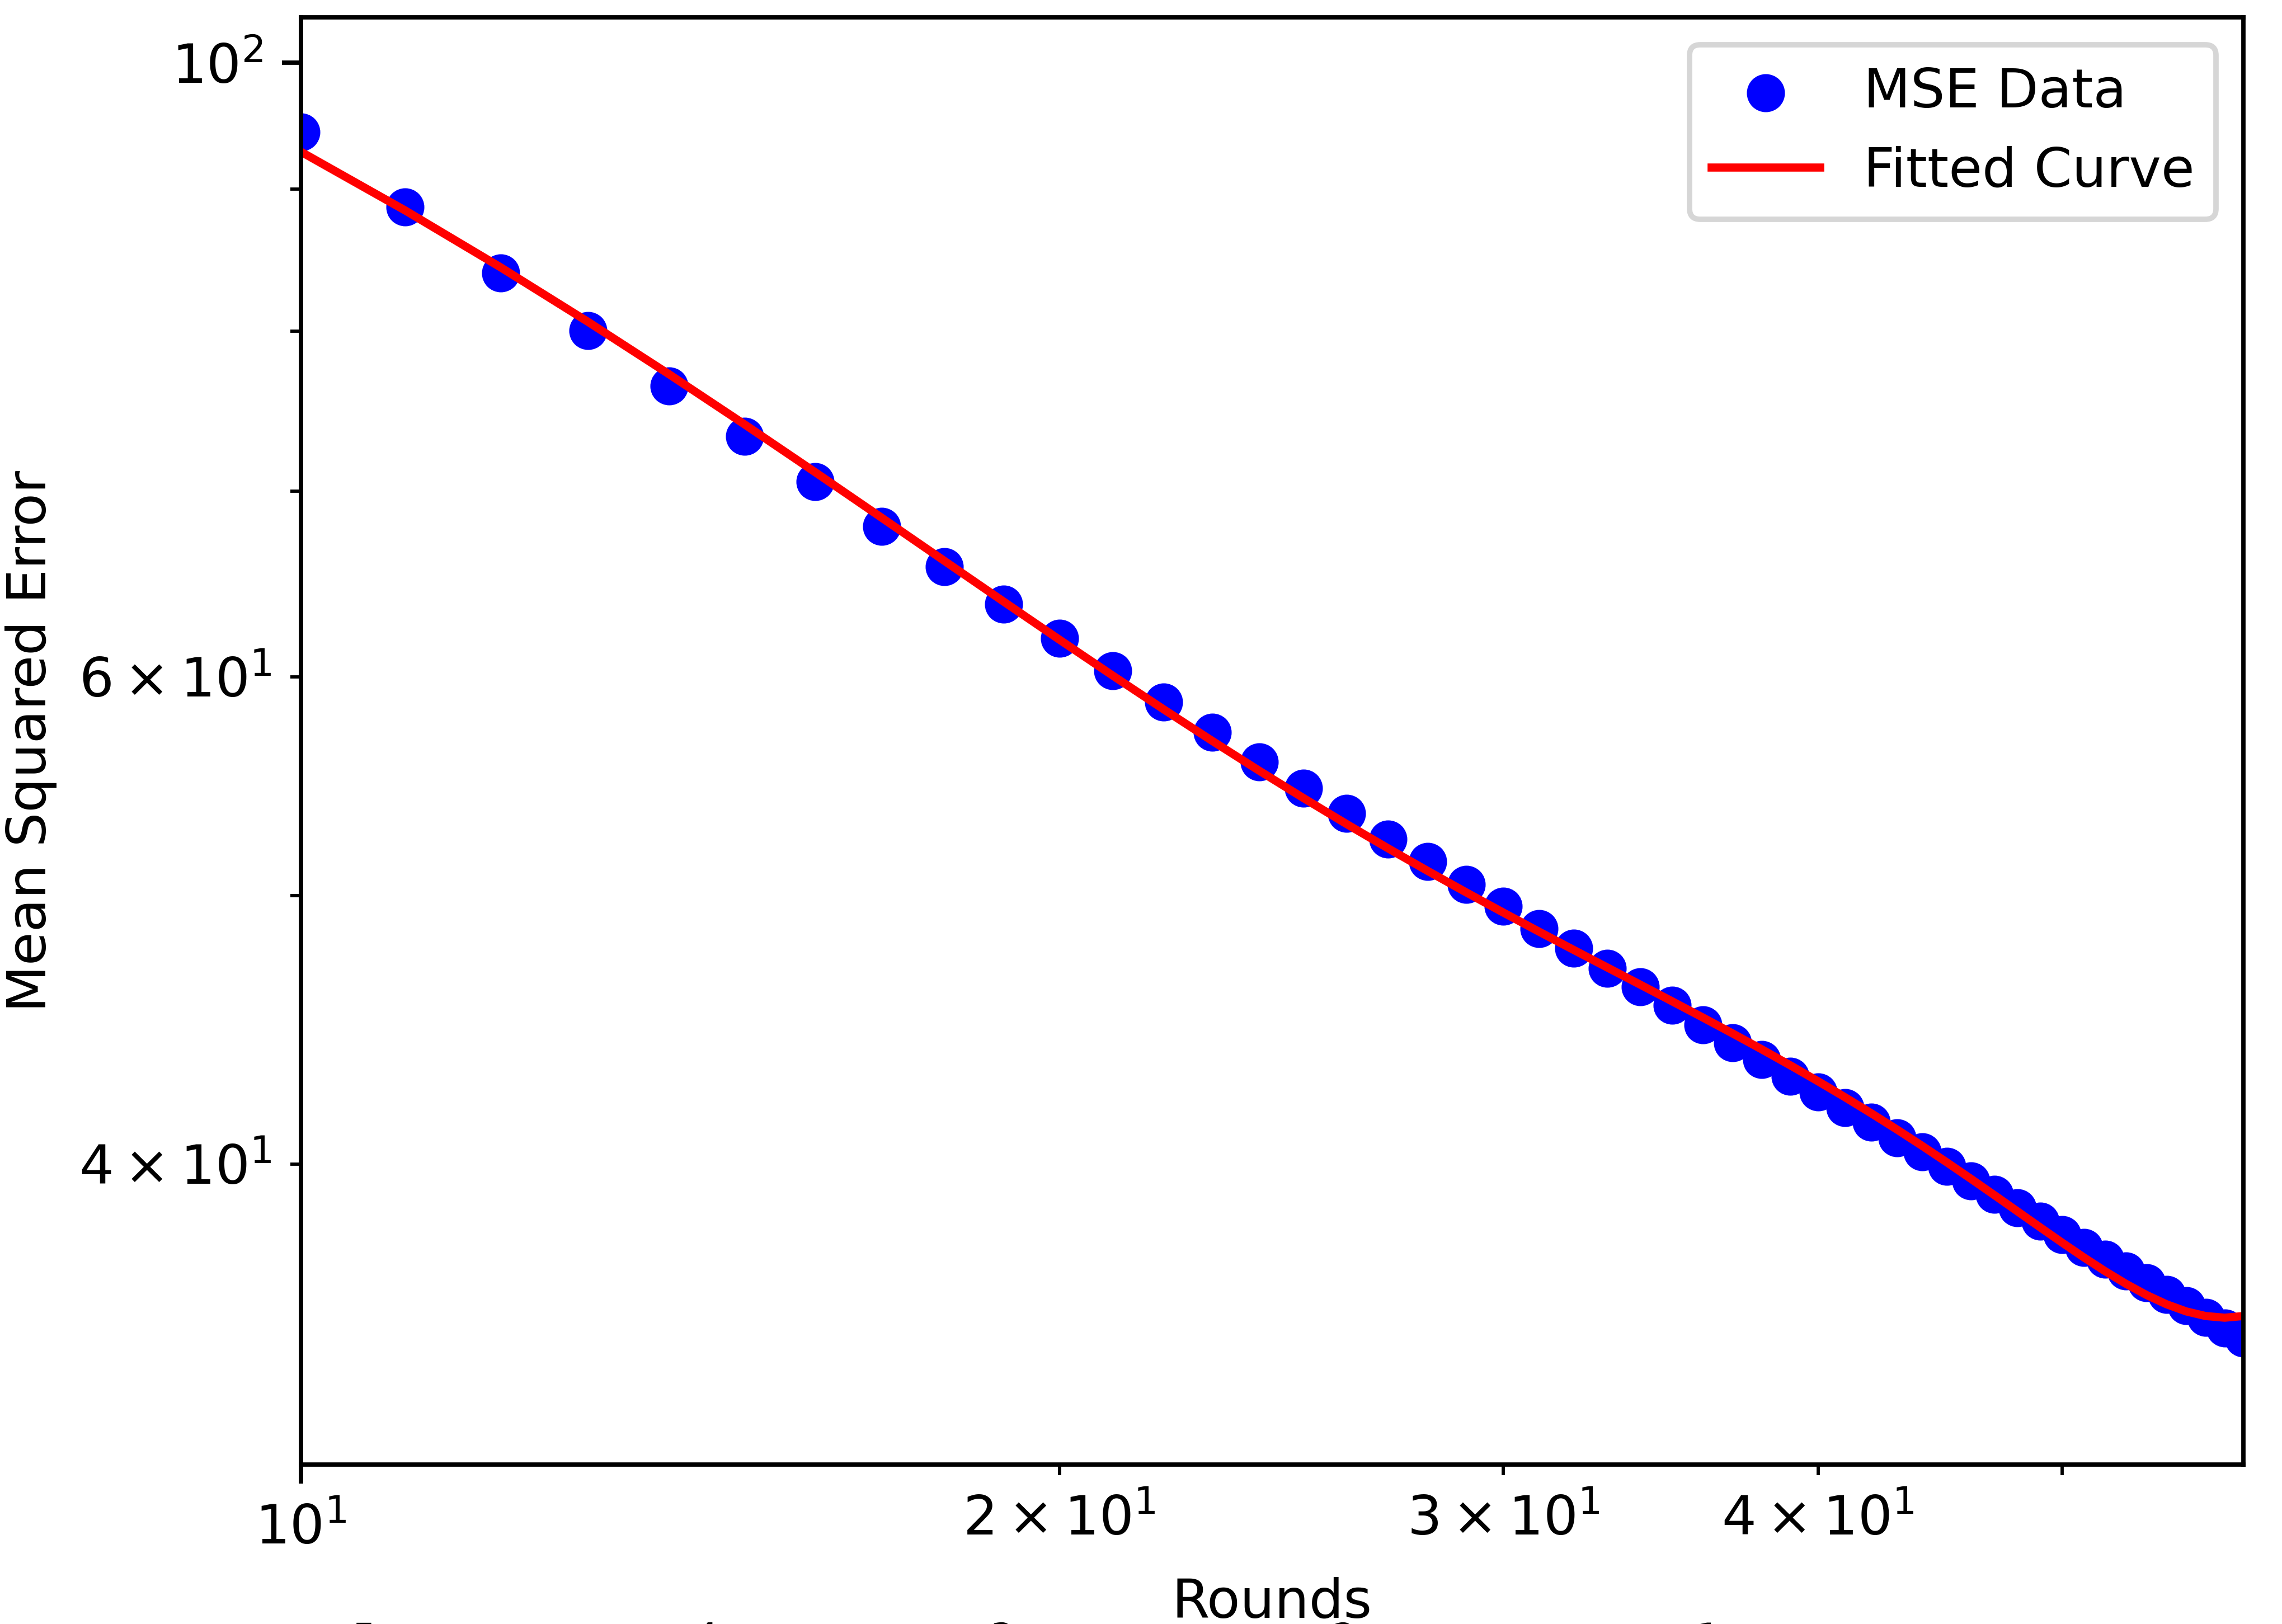
\includegraphics{figures/Simulation_outcomes/RingGraph/ATPPS/ATPPS_modelfitting_rounds_59_model_2.png}}
    \caption{Ring graph - polynomial regression fit: ATPPS}
    \label{fig:atppsRingModelFit}
\end{figure}
\begin{figure}
    \centering
    \scalebox{0.8}{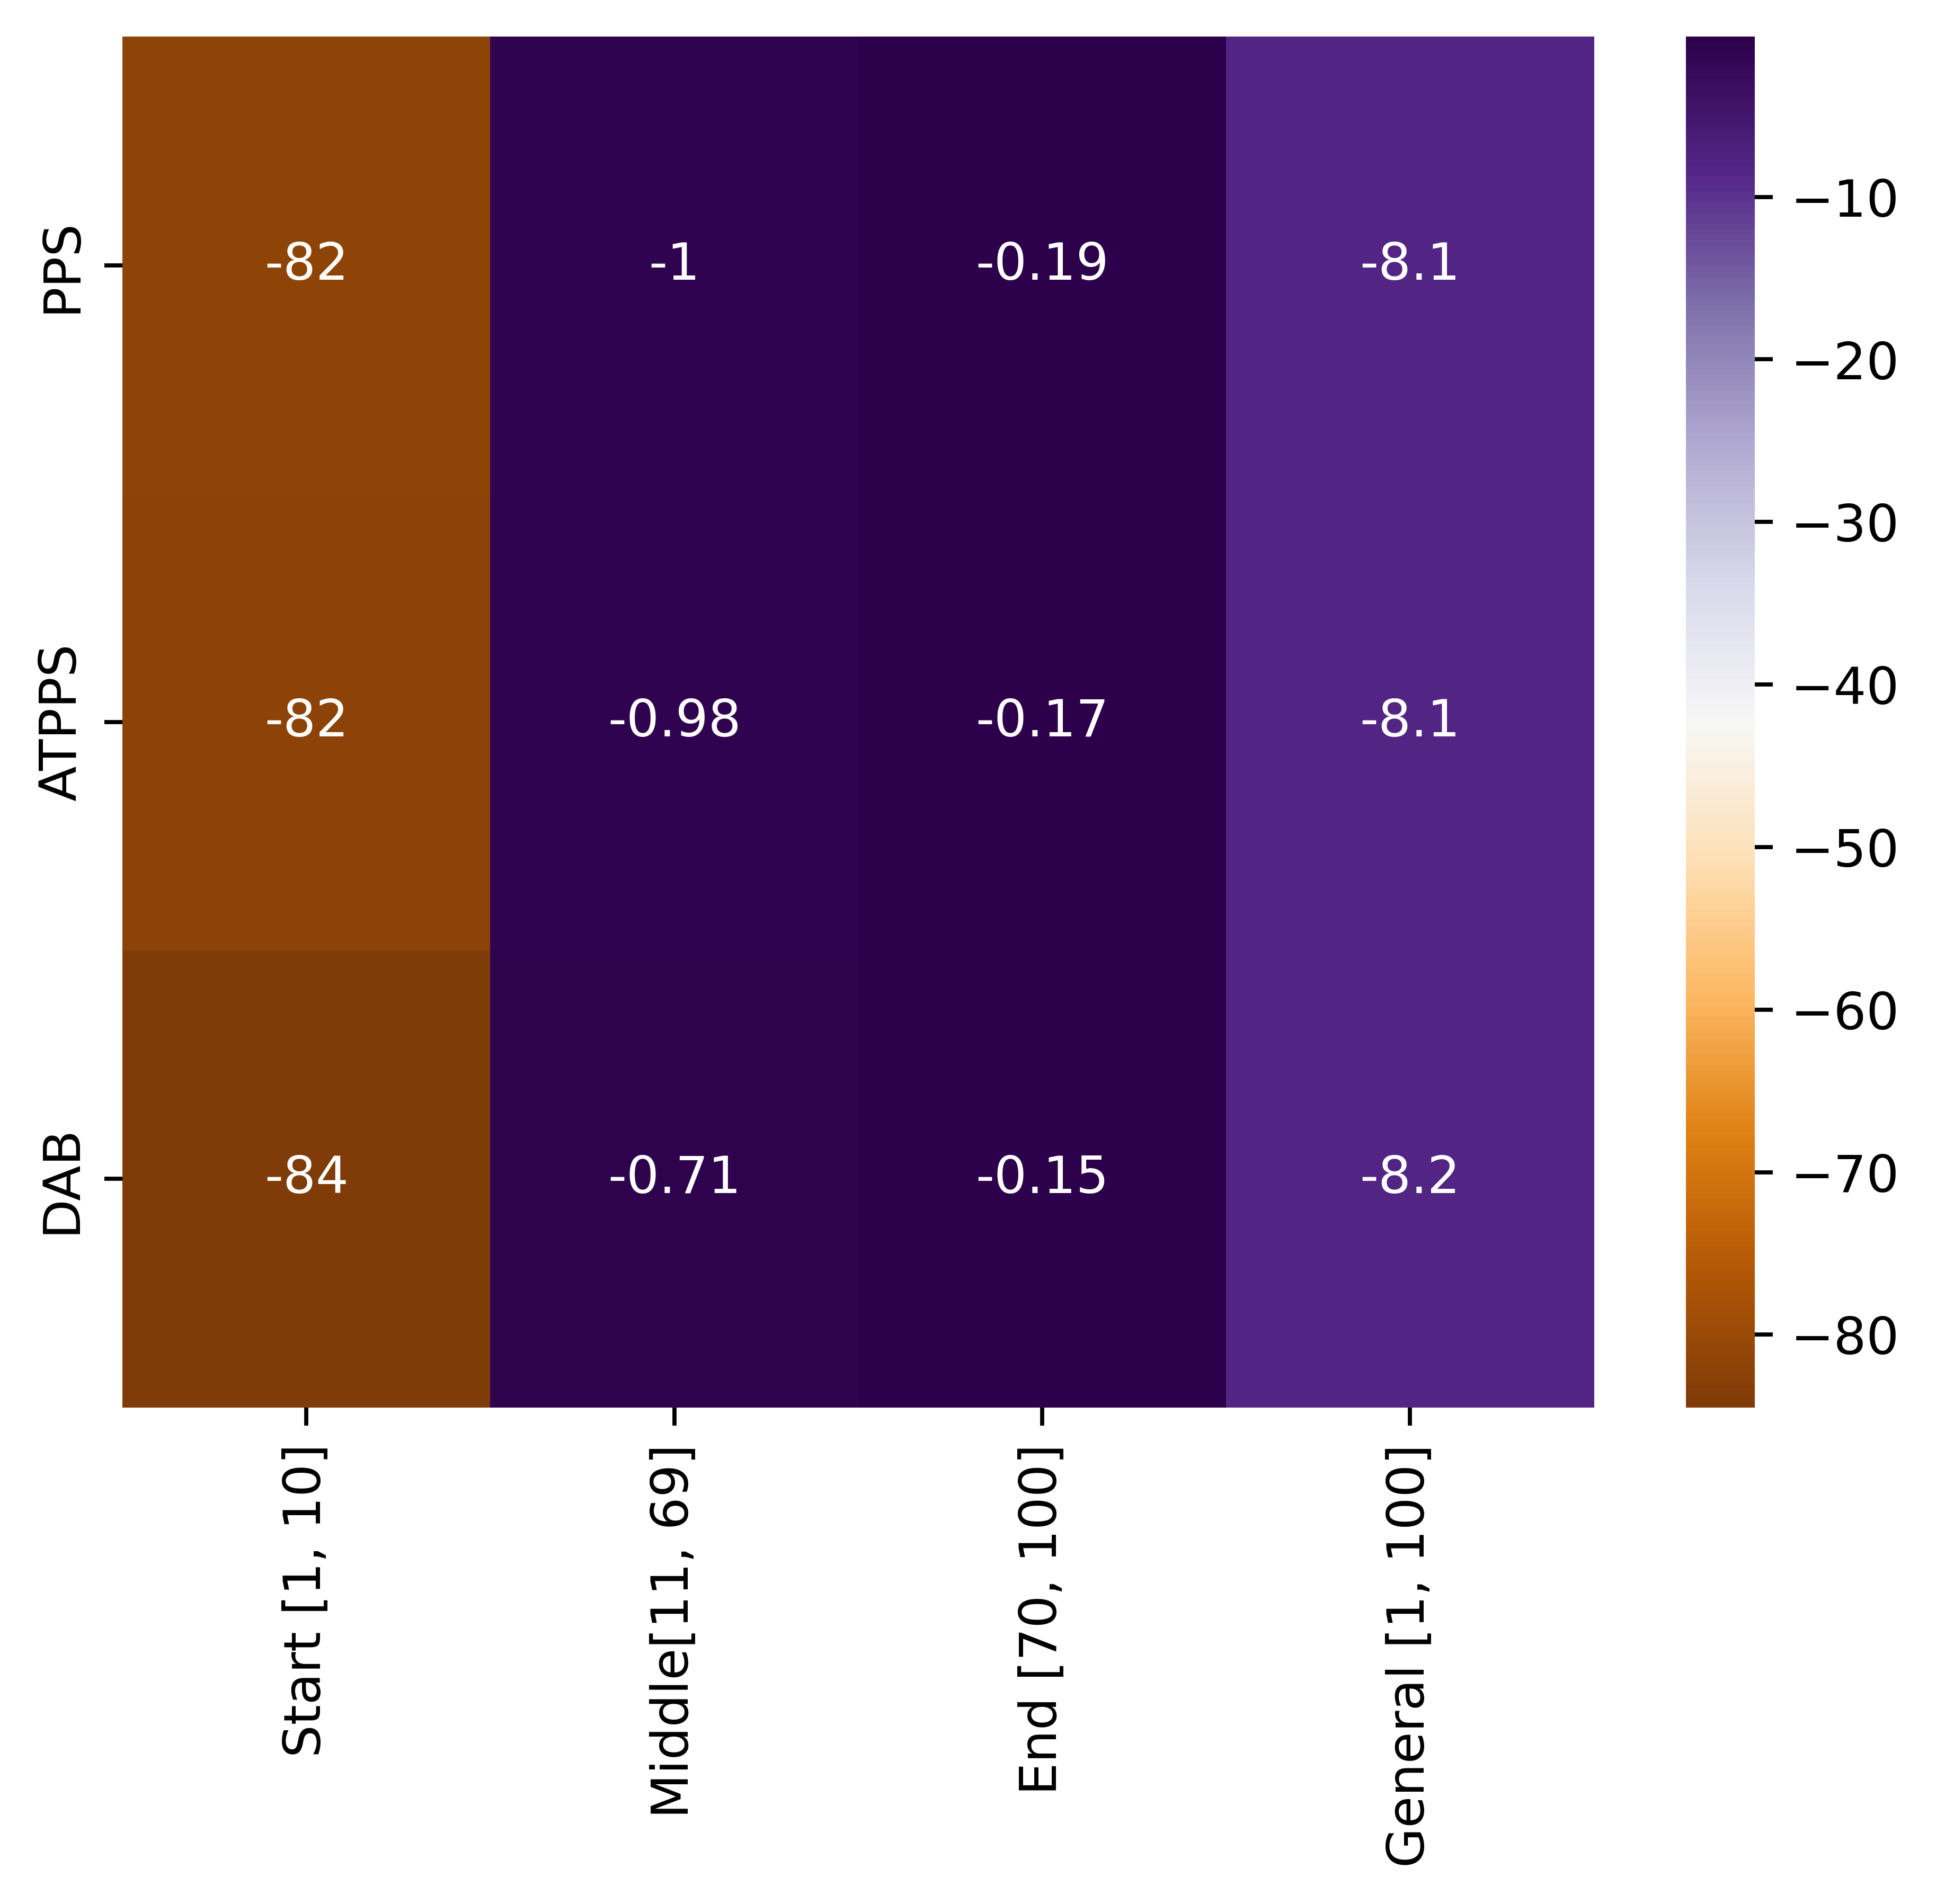
\includegraphics{figures/Simulation_outcomes/RingGraph/DAB_vs_PPS_vs_ATPPS_slopesheatmap_100rounds.png}}
    \caption{Ring graph: heat map of slopes per region}
    \label{fig:ringgraphslopes}
\end{figure}

\section{Torus Grid Graph}\label{sec:torusgridGraph}
Figure \ref{fig:torusMSEperRoundLogLog} shows the MSE reduction over rounds on a Torus Grid graph, plotted on a log-log scale. The DAB curve appears to have a slightly faster initial reduction compared to PPS' and ATPPS' curve in the beginning (rounds 1 to 7). The slope in this region is superior for the DAB algorithm with a value of -140 compared to -130 for the Push-Pull Sum based algorithms (figure \ref{fig:torusgraphslopes}). The PPS curve and ATPPS curve maintain nearly identical performances during the middle region (rounds 8 to 40), reducing MSE at a similar rate, with a slope of -1 for the PPS curve and -0.83 for the ATPPS curve. DAB shows a noticeable improvement of reducing the imbalance compared to both, PPS and ATPPS, achieving lower MSE values consistently. This suggests that DAB adapts more efficiently to the graph's structure during the intermediate (rounds in the middle) rounds. DAB continues to reduce MSE more effectively than the Push-Pull Sum based protocols in the end region (rounds 41 to 100). PPS and ATPPS exhibit convergence, but they lag behind the DAB algorithm in reaching minimal MSE. A Torus grid has more structured connectivity compared to a Star or Ring graph, allowing better distribution of loads via localized interactions. DAB's deterministic approach benefits from leveraging this regularity, leading to its superior performance. The ATPPS algorithm achieves a compromise solution in this scenario. It performs better than the PPS approach judging from the simulation outcomes, especially in later rounds, where the adaptiveness condition prevents "redundant" load transfers from happening and prioritizing load transfers that reduce the error impactfully.

The uniform neighborhood structure of Tori ensure that DAB's deterministic decisions (e.g., always choosing the minimal neighbor) are consistently effective across the graph. The algorithm does not suffer from random suboptimal decisions introduced by probabilistic neighbor choices, making it well-suited to the topology. Both PPS and ATPPS protocols rely on randomly selecting a neighbor for load exchange. While this randomness is beneficial in irregular or dense graphs (e.g., Star or Complete graphs), it is less effective in structured topologies compared to the DAB like a Torus Grid. The Push-Pull Sum based algorithms do not always target the most unbalanced areas. This means that load propagation can sometimes "stall" in certain regions, requiring more rounds to achieve global balance. The ATTPS draws its benefit over the PPS (especially in later rounds) by deciding which option of the available subset is the best. The discrepancy between the two load balancing algorithms widens in the last few rounds as trades between two nodes with higher load differences are more impactful once the network is already heavily balanced.

The fitted polynomial curve of degree 5 matches the MSE data for DAB effectively, capturing the non-linear dynamics during rounds 10 to 39 following the equation: $MSE_r=-1.35\times 10^{-6}r^{5}+ 1.89\times 10^{-4}r^{4}-0.01r^{3}+0.30r^{2}-4.6r+34.10$ (figure \ref{fig:dabTorusModelFit} a)). This suggests that in the early rounds (rounds 10 to 39), the MSE reduction follows a complex pattern due to the DAB's optimization mechanism, such as its focus on minimizing neighbors loads dynamically. The higher degree captures these dynamics with more precision than simpler models. In later rounds the performance of the DAB can still be captured by a polynomial curve of degree 3 with equation: $MSE_r=-6.01\times 10^{-06}r^{3}+1.66\times 10^{-3}r^{2}-0.16r+6$ (figure \ref{fig:dabTorusModelFit} b)). By this stage, the load balancing has stabilized, and the reduction in MSE is more linear or gradual. A lower-degree polynomial suffices for rounds 40 to 100 since the dynamics are simpler compared to the earlier rounds. The curve behavior for the PPS and ATPPS are similar to that of the DAB curve expressed for rounds 10 to 39 by the equations: $MSE_r=-5.54\times 10^{-6}r^{5}+7.65\times 10^{-4}r^{4}-0.04r^{3}+1.16r^{2}-16.81r+112.86$ for the PPS (figure \ref{fig:ppsTorusModelFit} a)) and: $MSE_r = -3.65 \times 10^{-6}r^{5} + 5.16 \times 10^{-4}r^{4} - 0.03r^{3} + 0.83r^{2} - 12.52r + 88.16$ for the ATPPS (figure \ref{fig:atppstorusModelFit} a)). The equations that describe the behavior of the two Push-Pull Sum based algorithms are fitted for the rounds 40 to 100 for the PPS is: $MSE_r = -1.15 \times 10^{-5}r^{3} + 3.205\times 10^{-3}r^{2} - 0.33r + 13.72$ (figure \ref{fig:ppsTorusModelFit} b))and for the ATPPS is: $MSE_r = -9.99 \times 10^{-6}r^{3} + 2.8034\times 10^{-3}r^{2} - 0.28r + 11.29$ (figure \ref{fig:atppstorusModelFit} b)). 
\begin{figure}[]
    \centering
    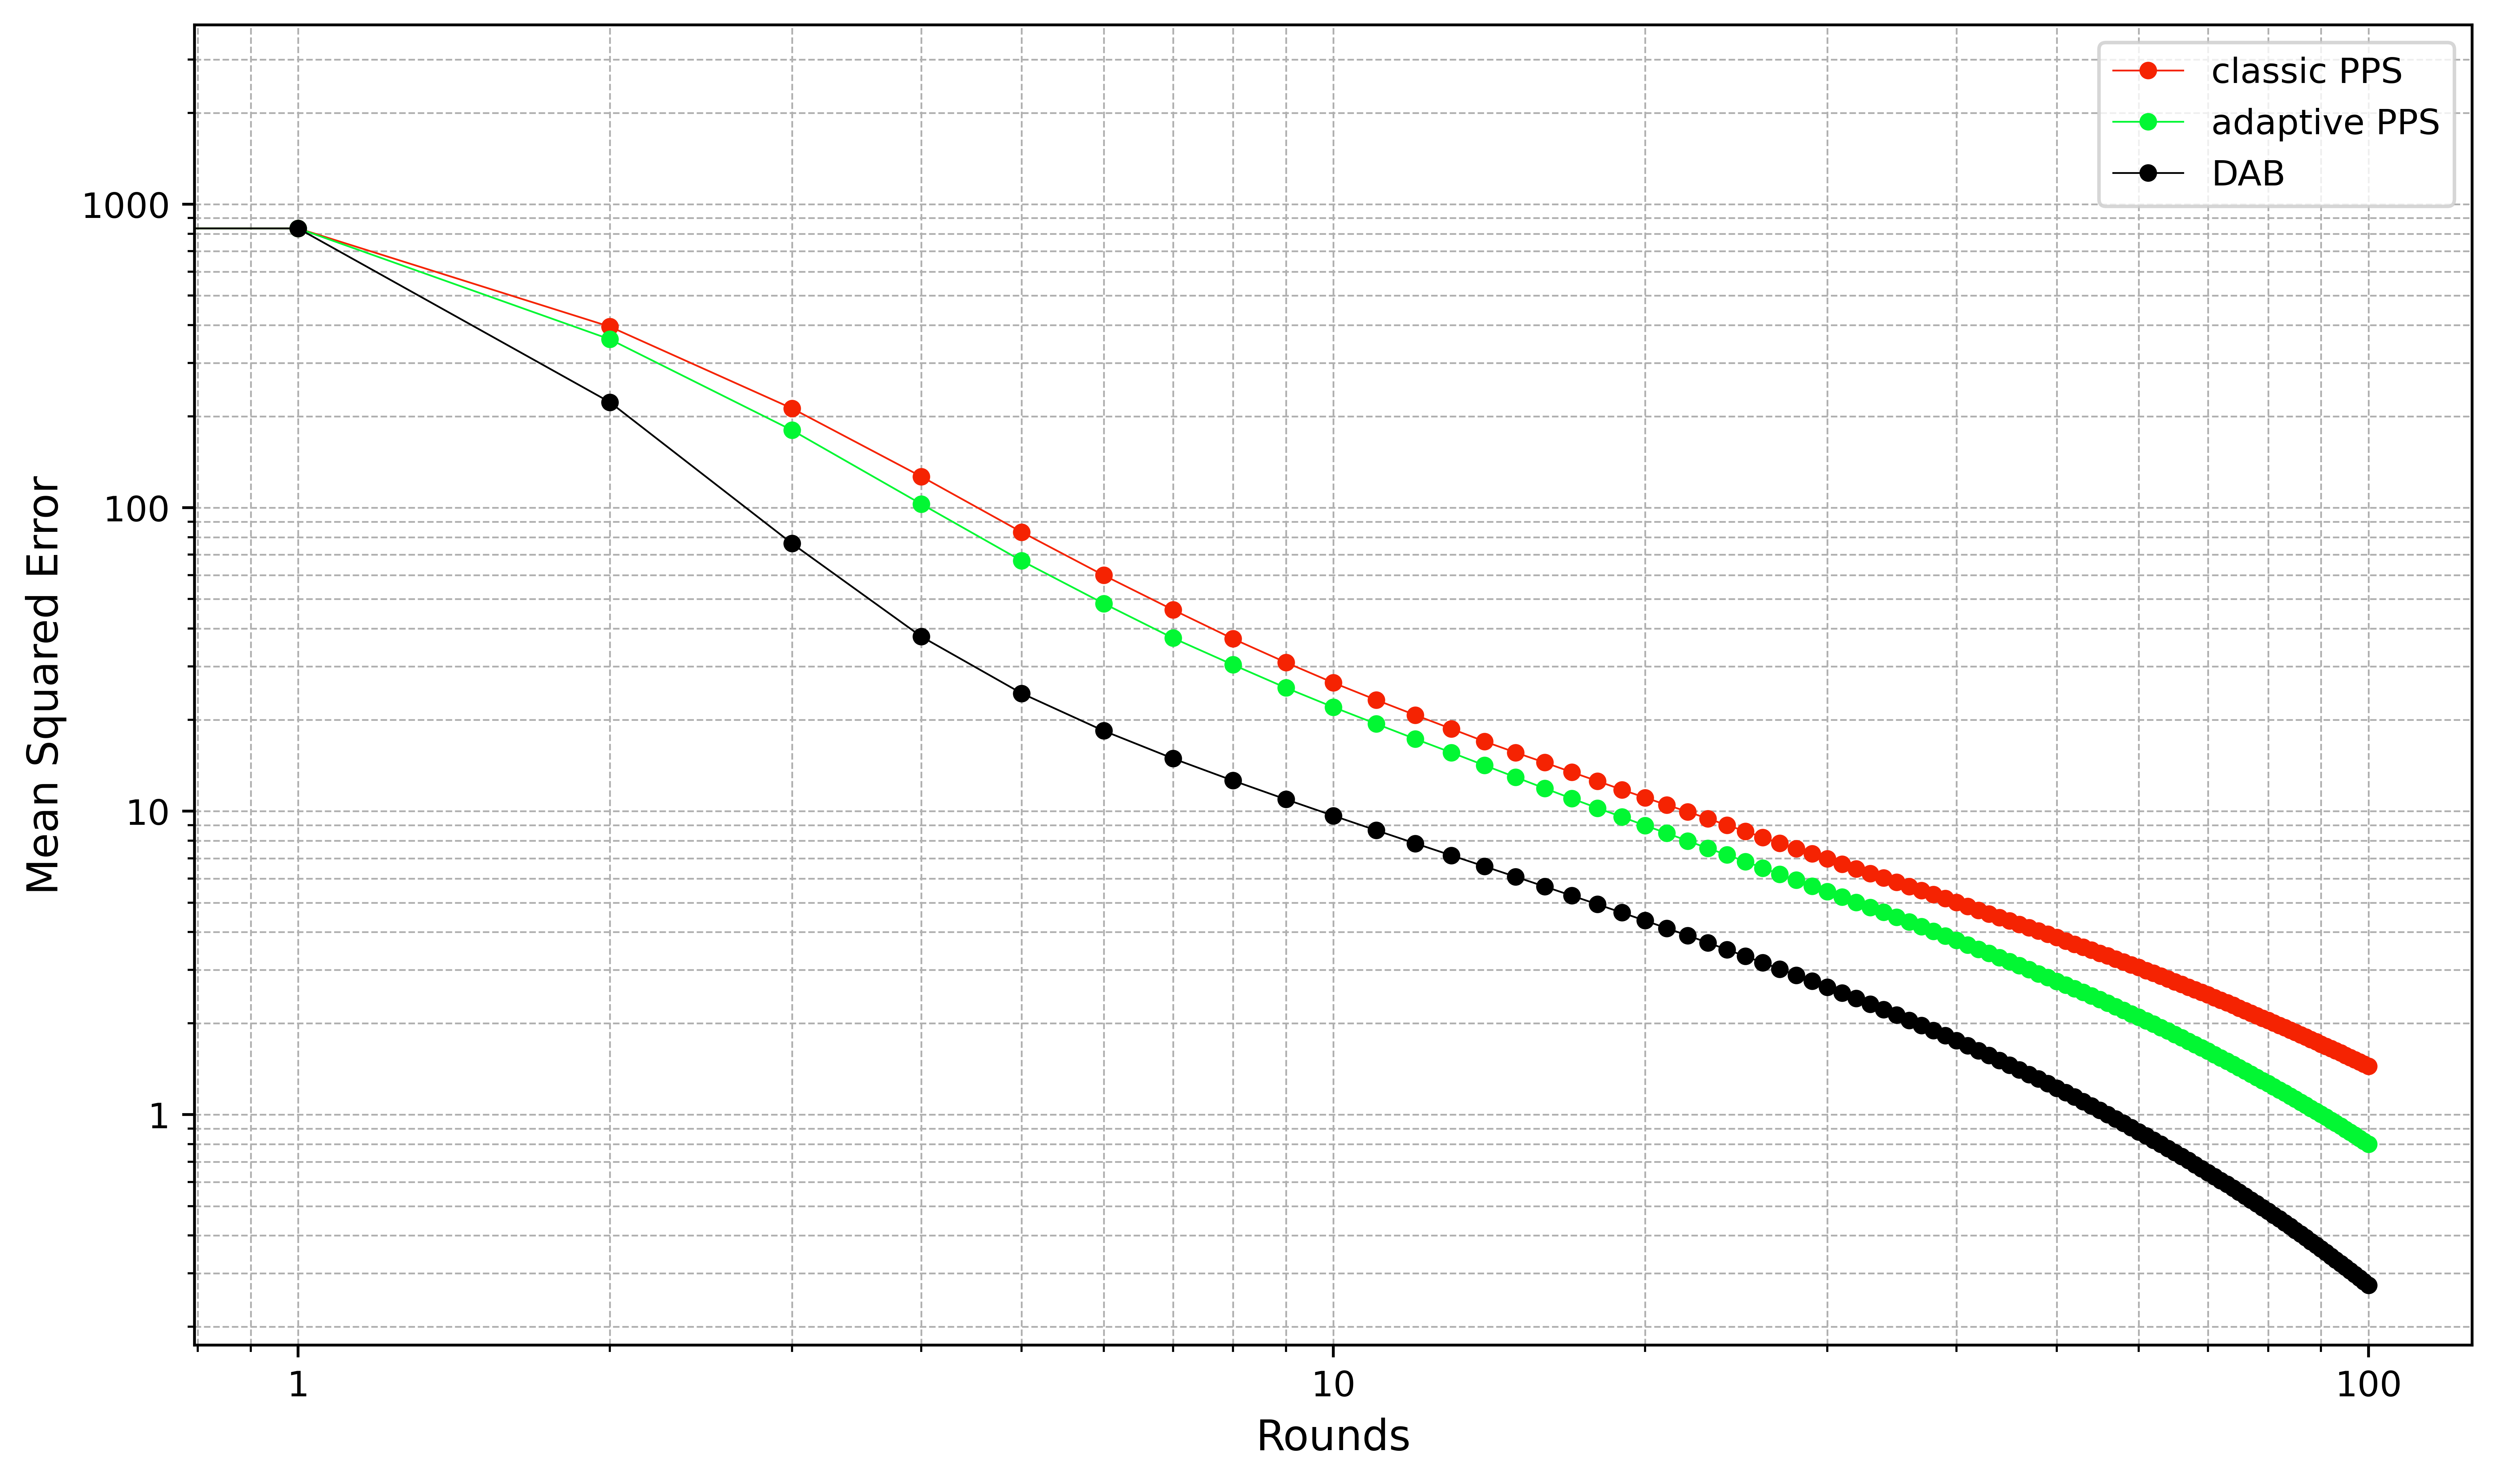
\includegraphics[width=\linewidth]{figures/Simulation_outcomes/TorusGridGraph/DAB_vs_PPS_TGG_r100_n1024_averaged_loglog.png}
    \caption{Torus Grid: mean squared error per rounds (log-log)}
    \label{fig:torusMSEperRoundLogLog}
\end{figure}
\begin{figure}[!ht]
     \centering
         \subfloat[]{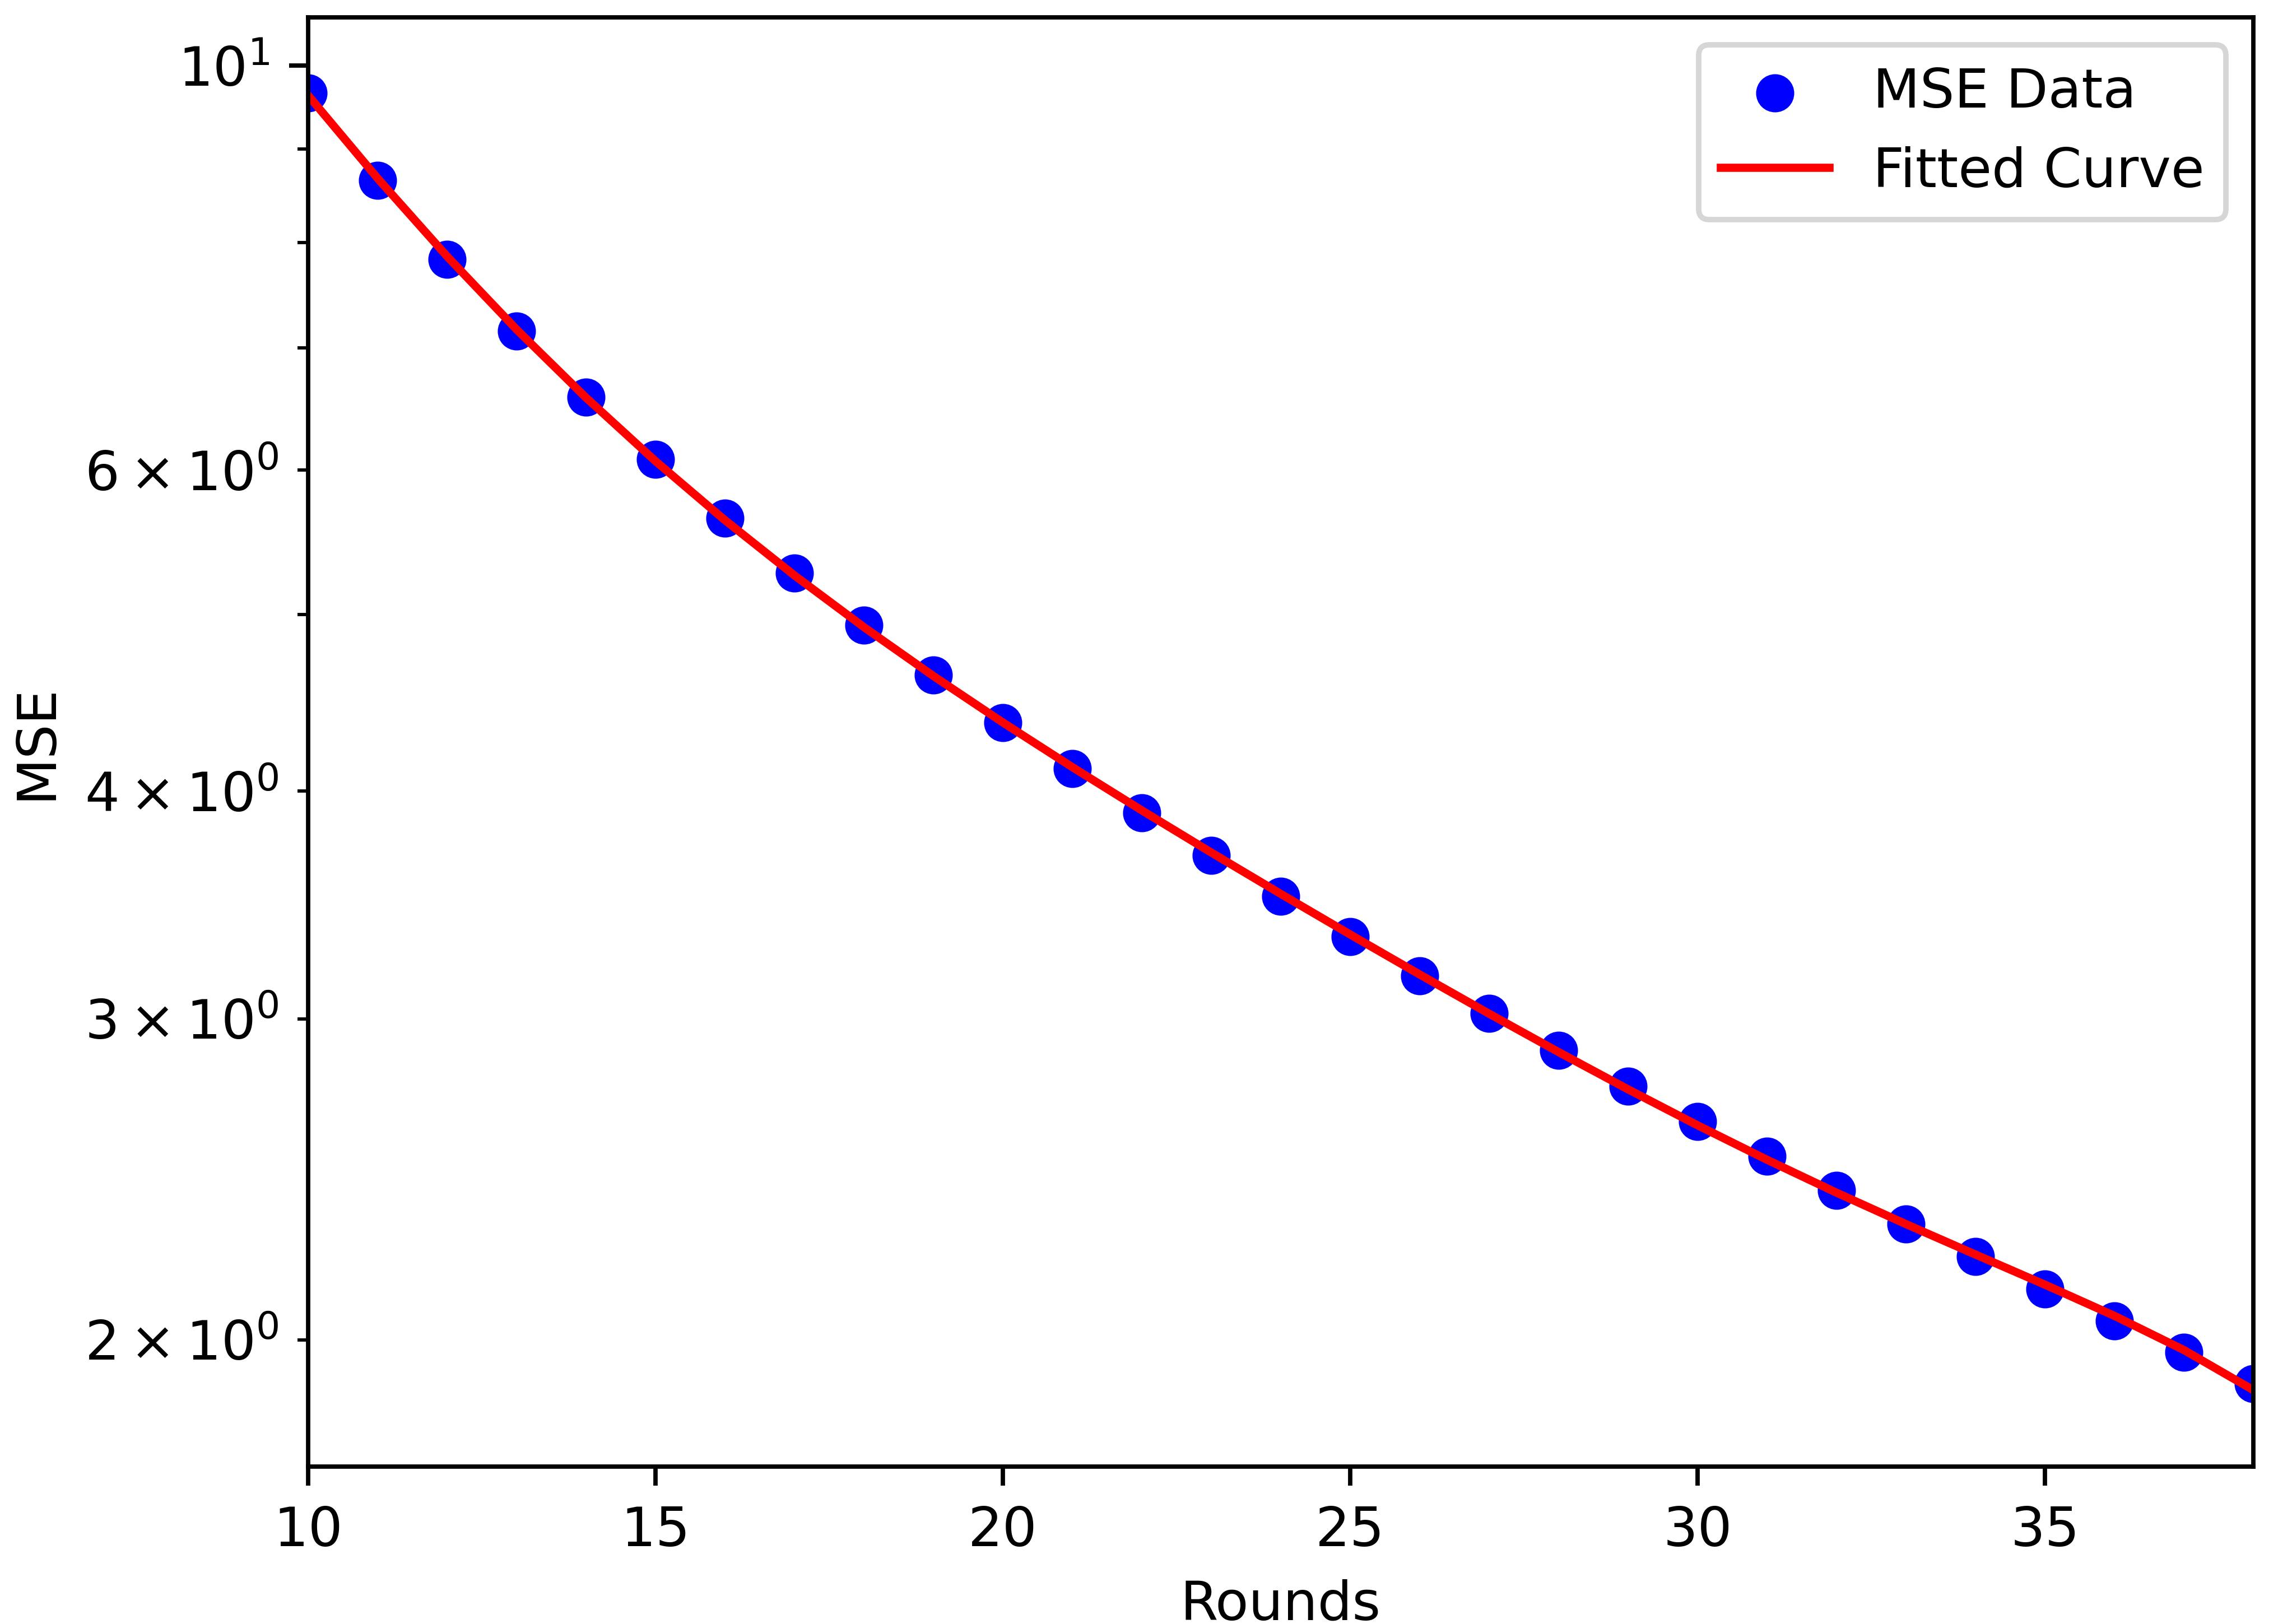
\includegraphics[width=0.49\linewidth]{figures/Simulation_outcomes/TorusGridGraph/DAB/DAB_modelfitting_rounds_38_model_2.png}}
     \hfil
         \subfloat[]{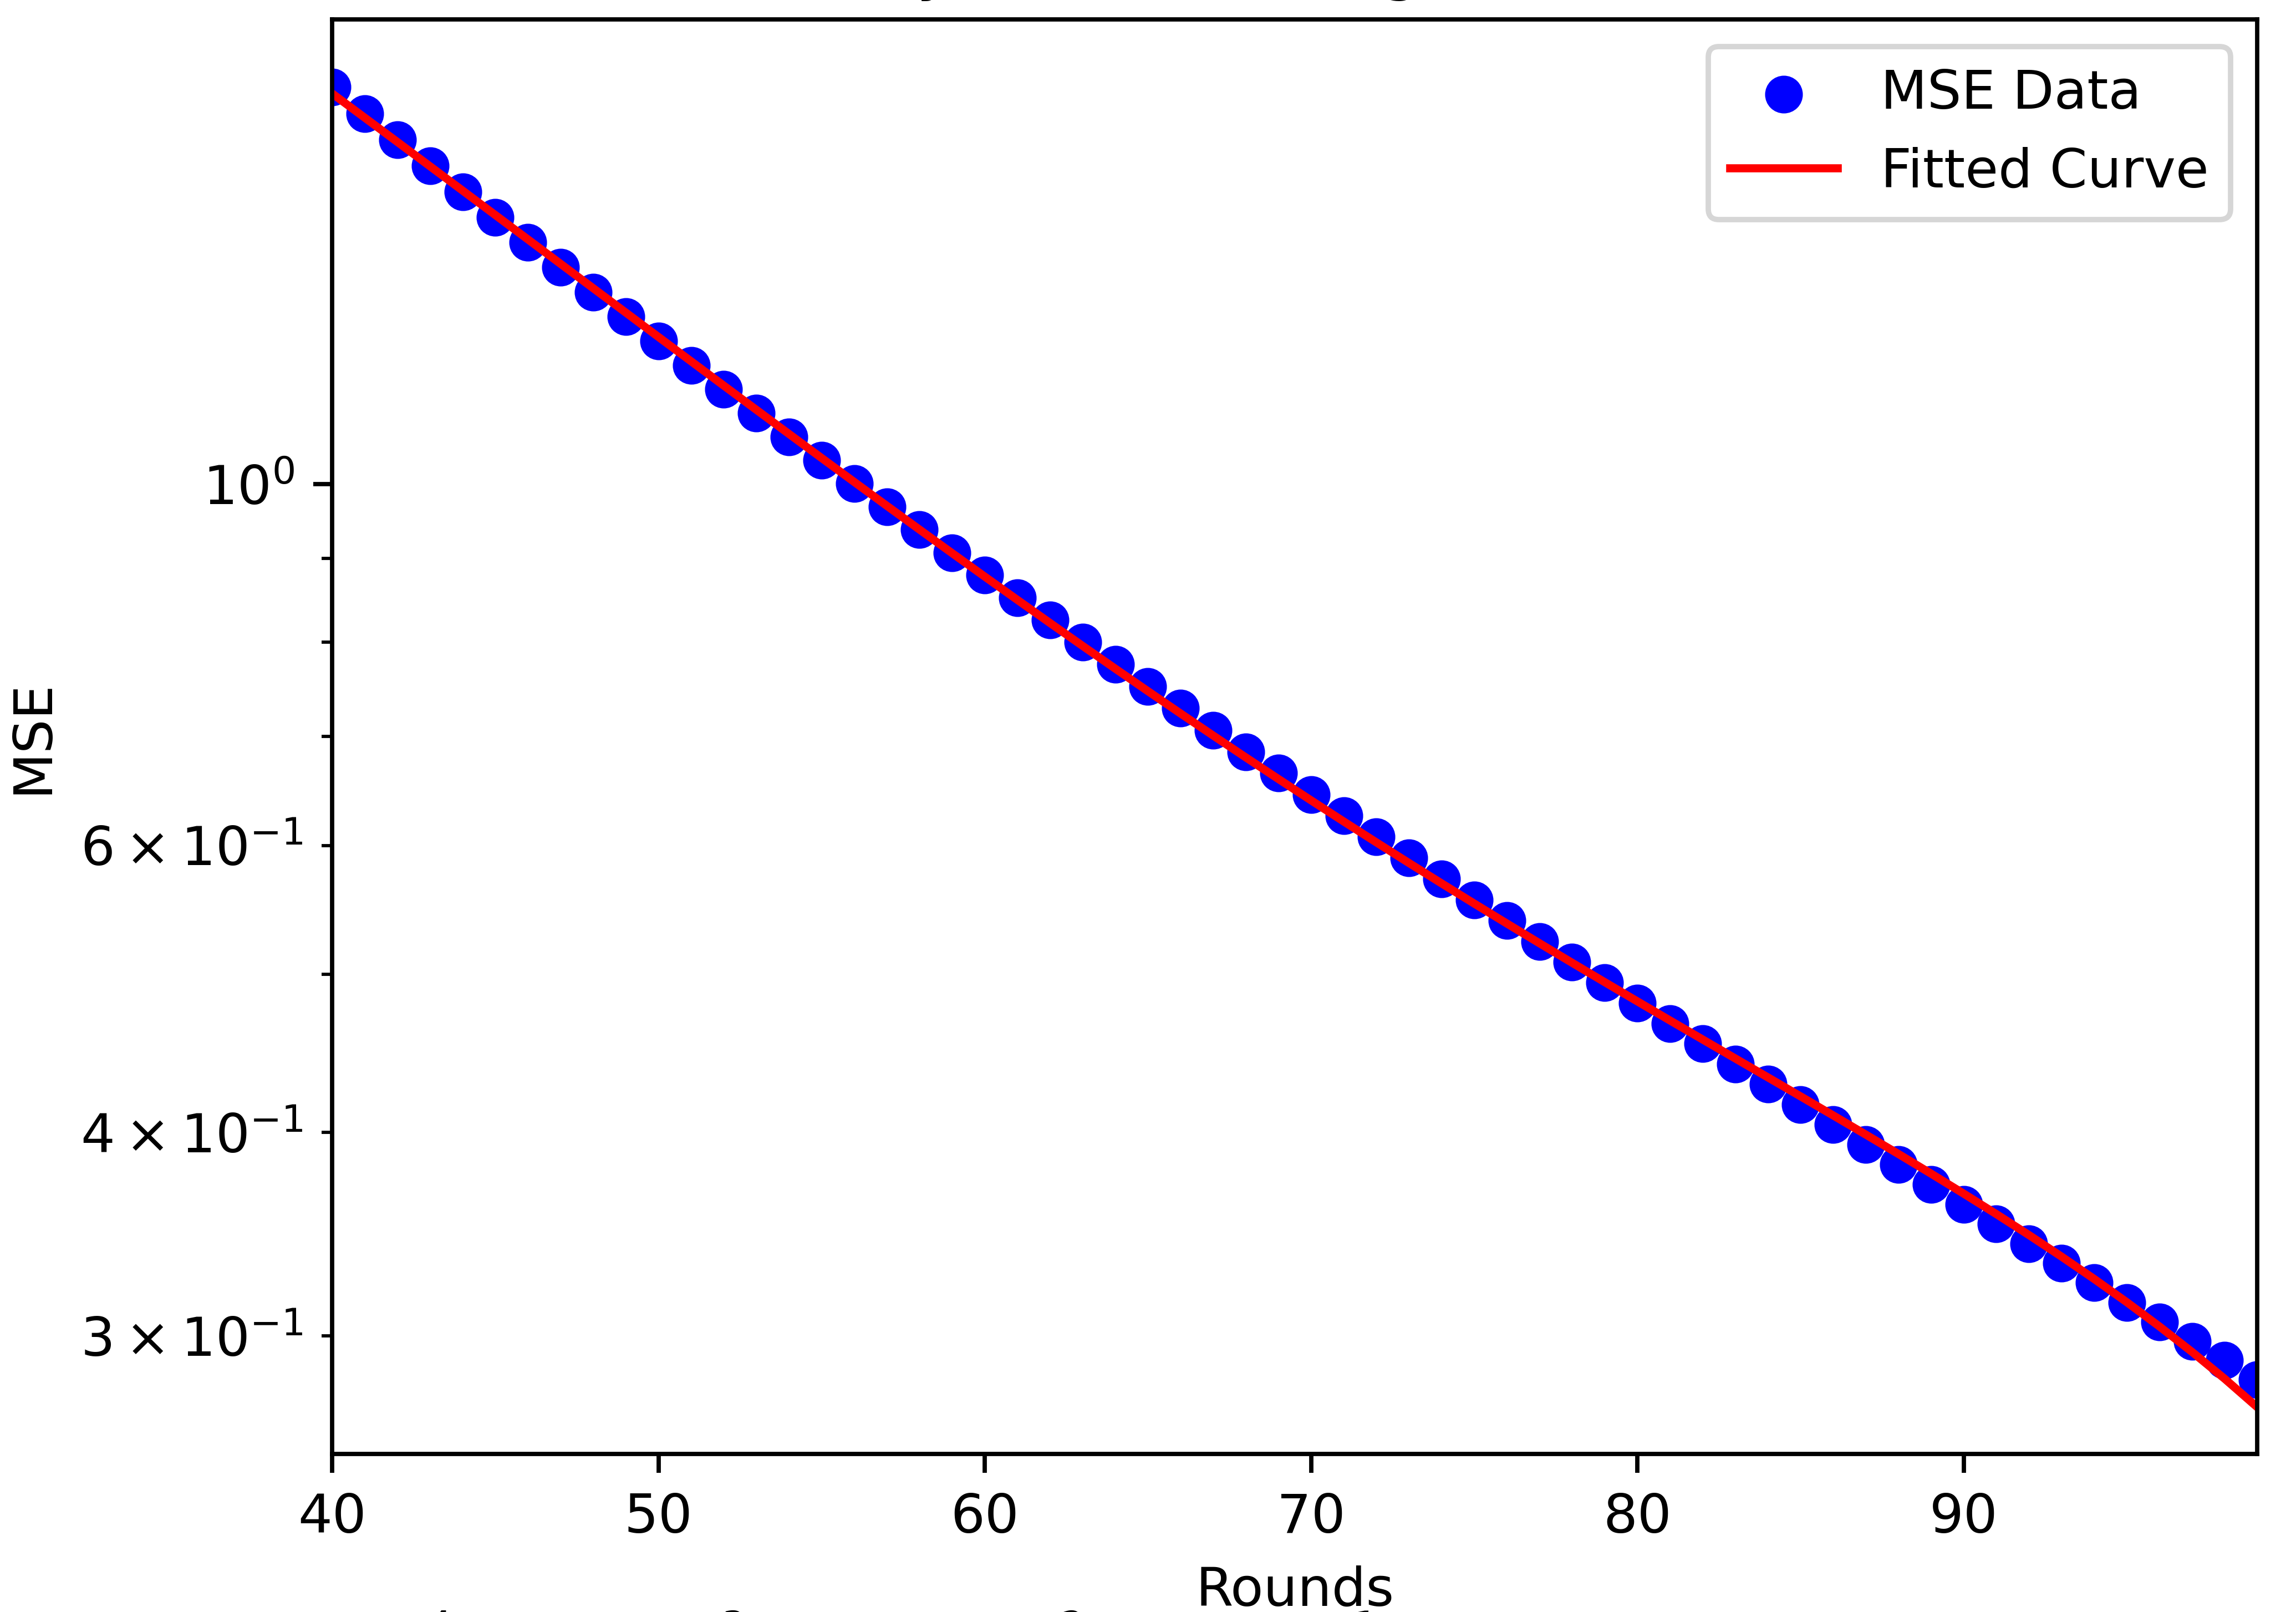
\includegraphics[width=0.49\linewidth]{figures/Simulation_outcomes/TorusGridGraph/DAB/DAB_modelfitting_rounds_99_model_2.png}}
     \caption{Torus Grid - polynomial regression fit: DAB; rounds 10-39 and 40-100}
         \label{fig:dabTorusModelFit}
 \end{figure}
 \begin{figure}[!ht]
     \centering
         \subfloat[]{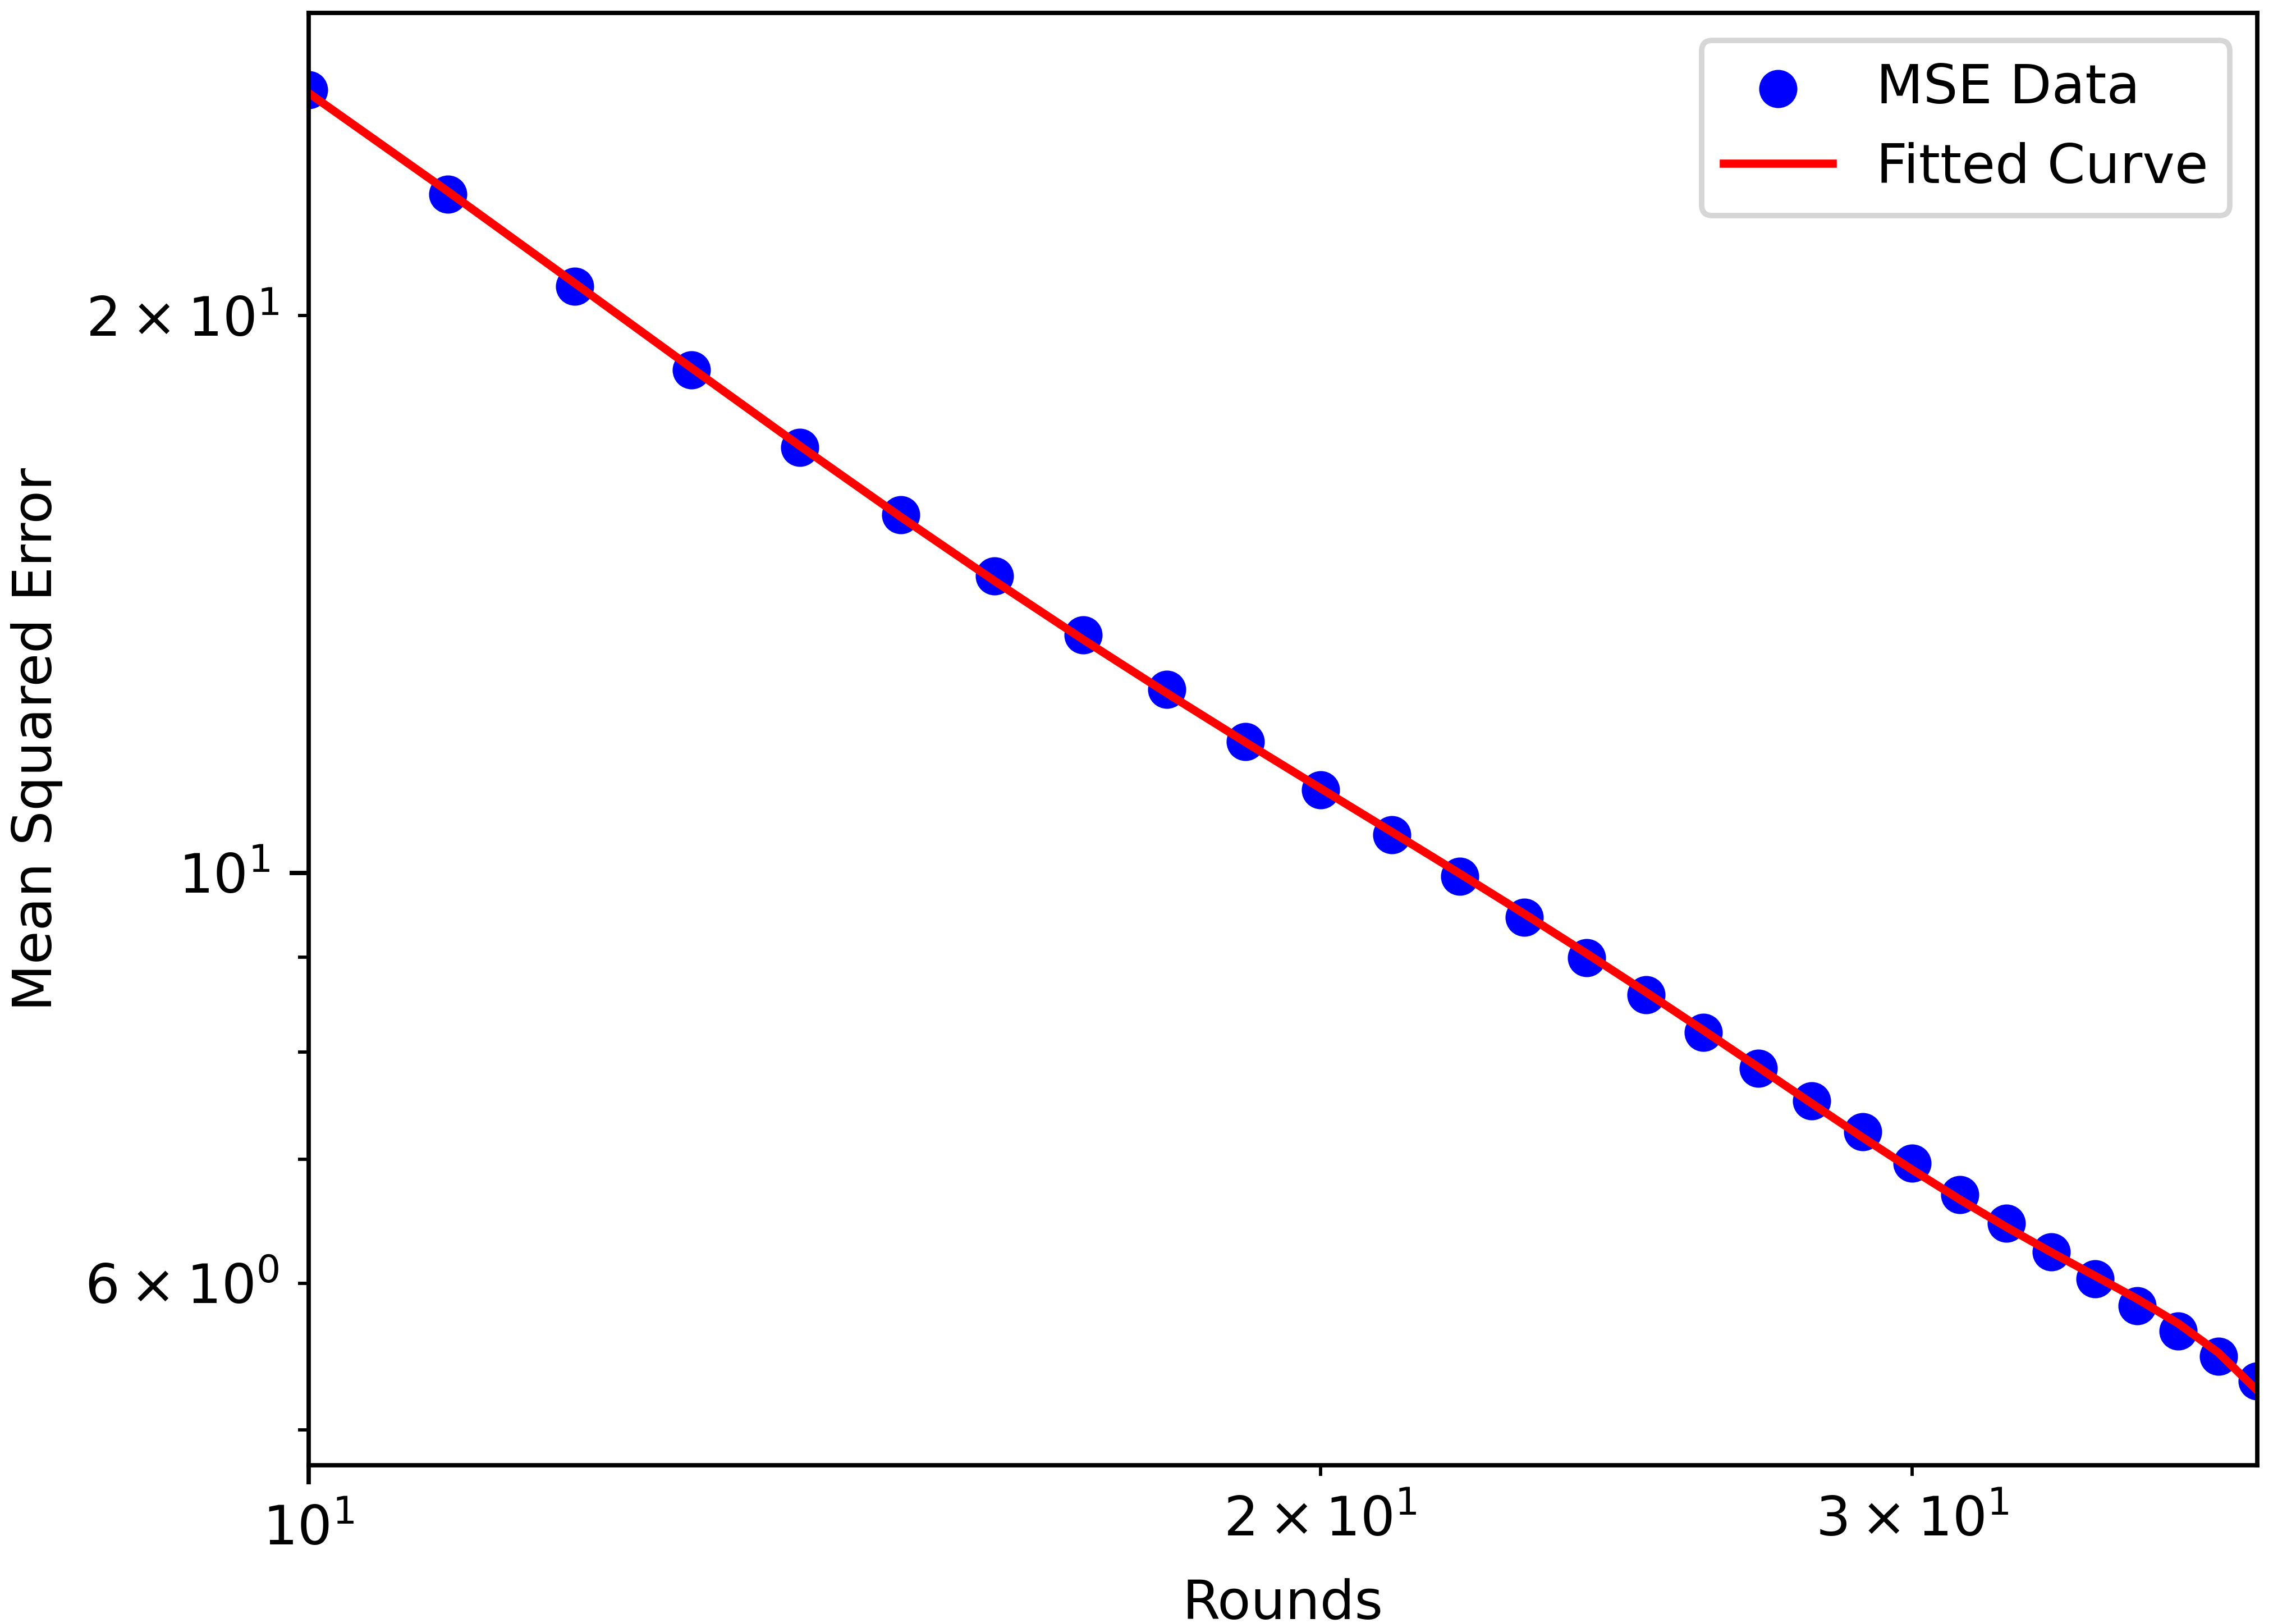
\includegraphics[width=0.49\linewidth]{figures/Simulation_outcomes/TorusGridGraph/PPS/PPS_modelfitting_rounds_38_model_2.png}}
     \hfil
         \subfloat[]{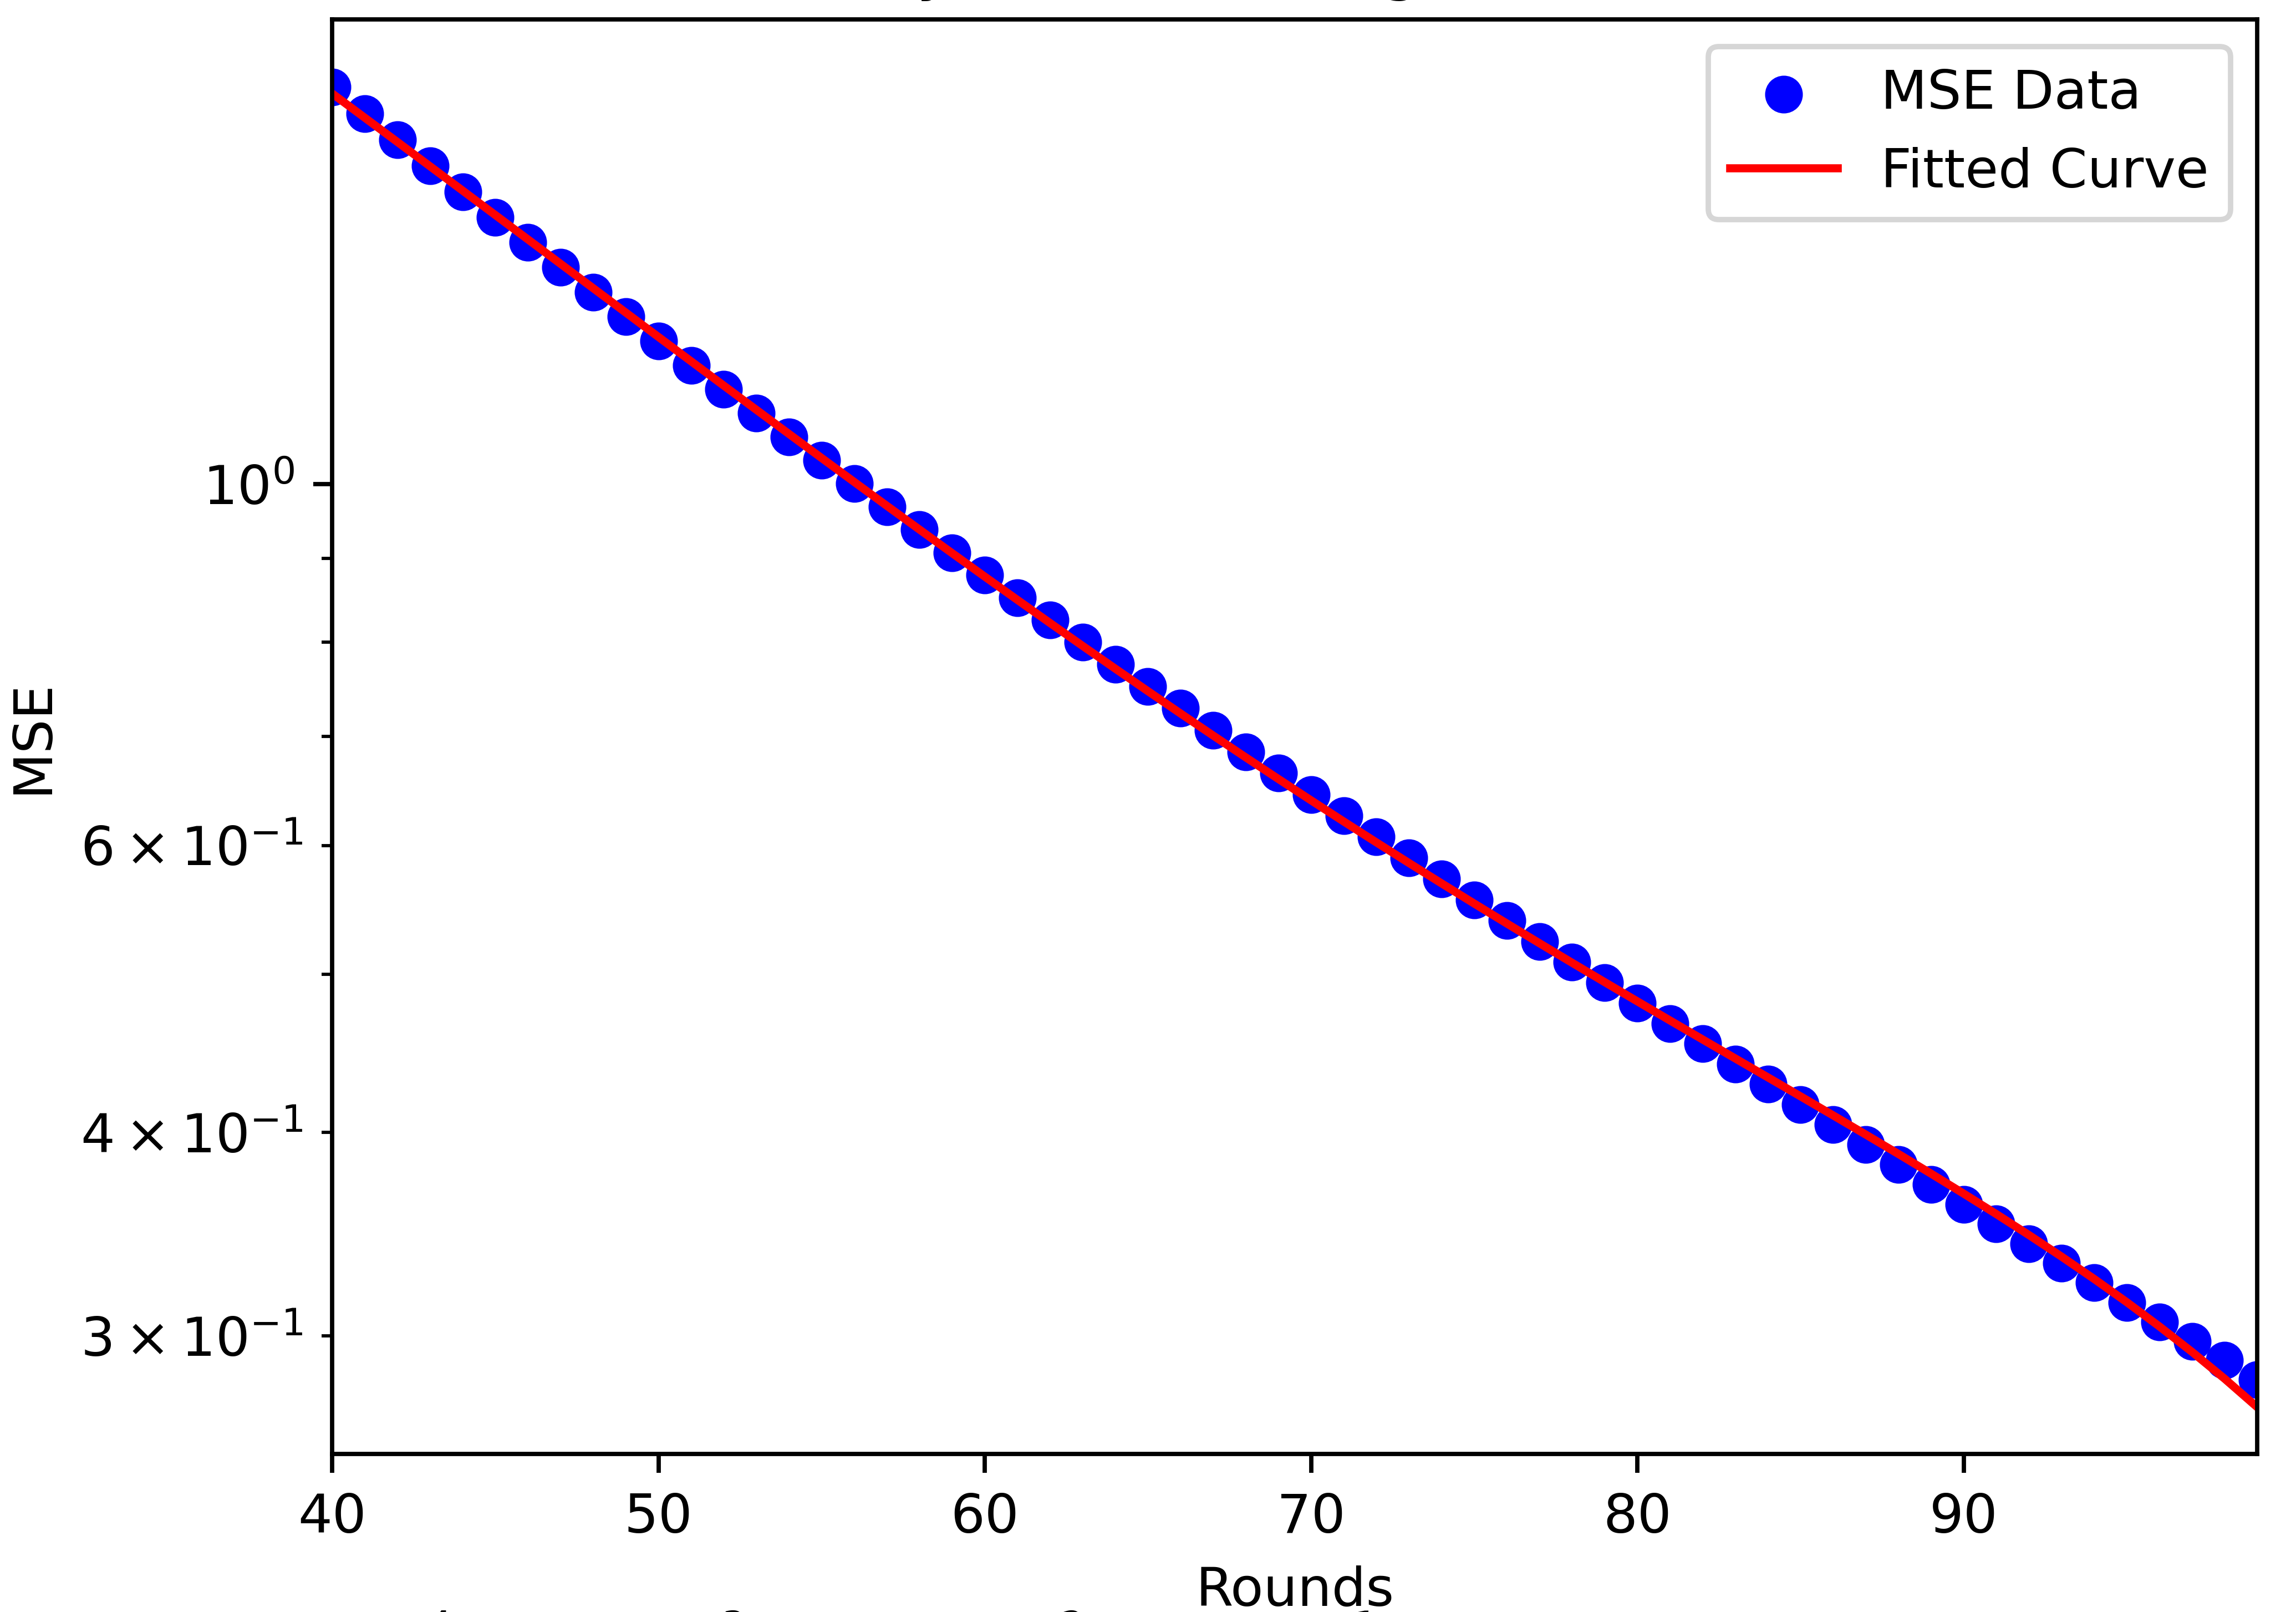
\includegraphics[width=0.49\linewidth]{figures/Simulation_outcomes/TorusGridGraph/DAB/DAB_modelfitting_rounds_99_model_2.png}}
     \caption{Torus Grid - polynomial regression fit: PPS; rounds 10-39 and 40-100}
         \label{fig:ppsTorusModelFit}
 \end{figure}
\begin{figure}[!ht]
    \centering
        \subfloat[]{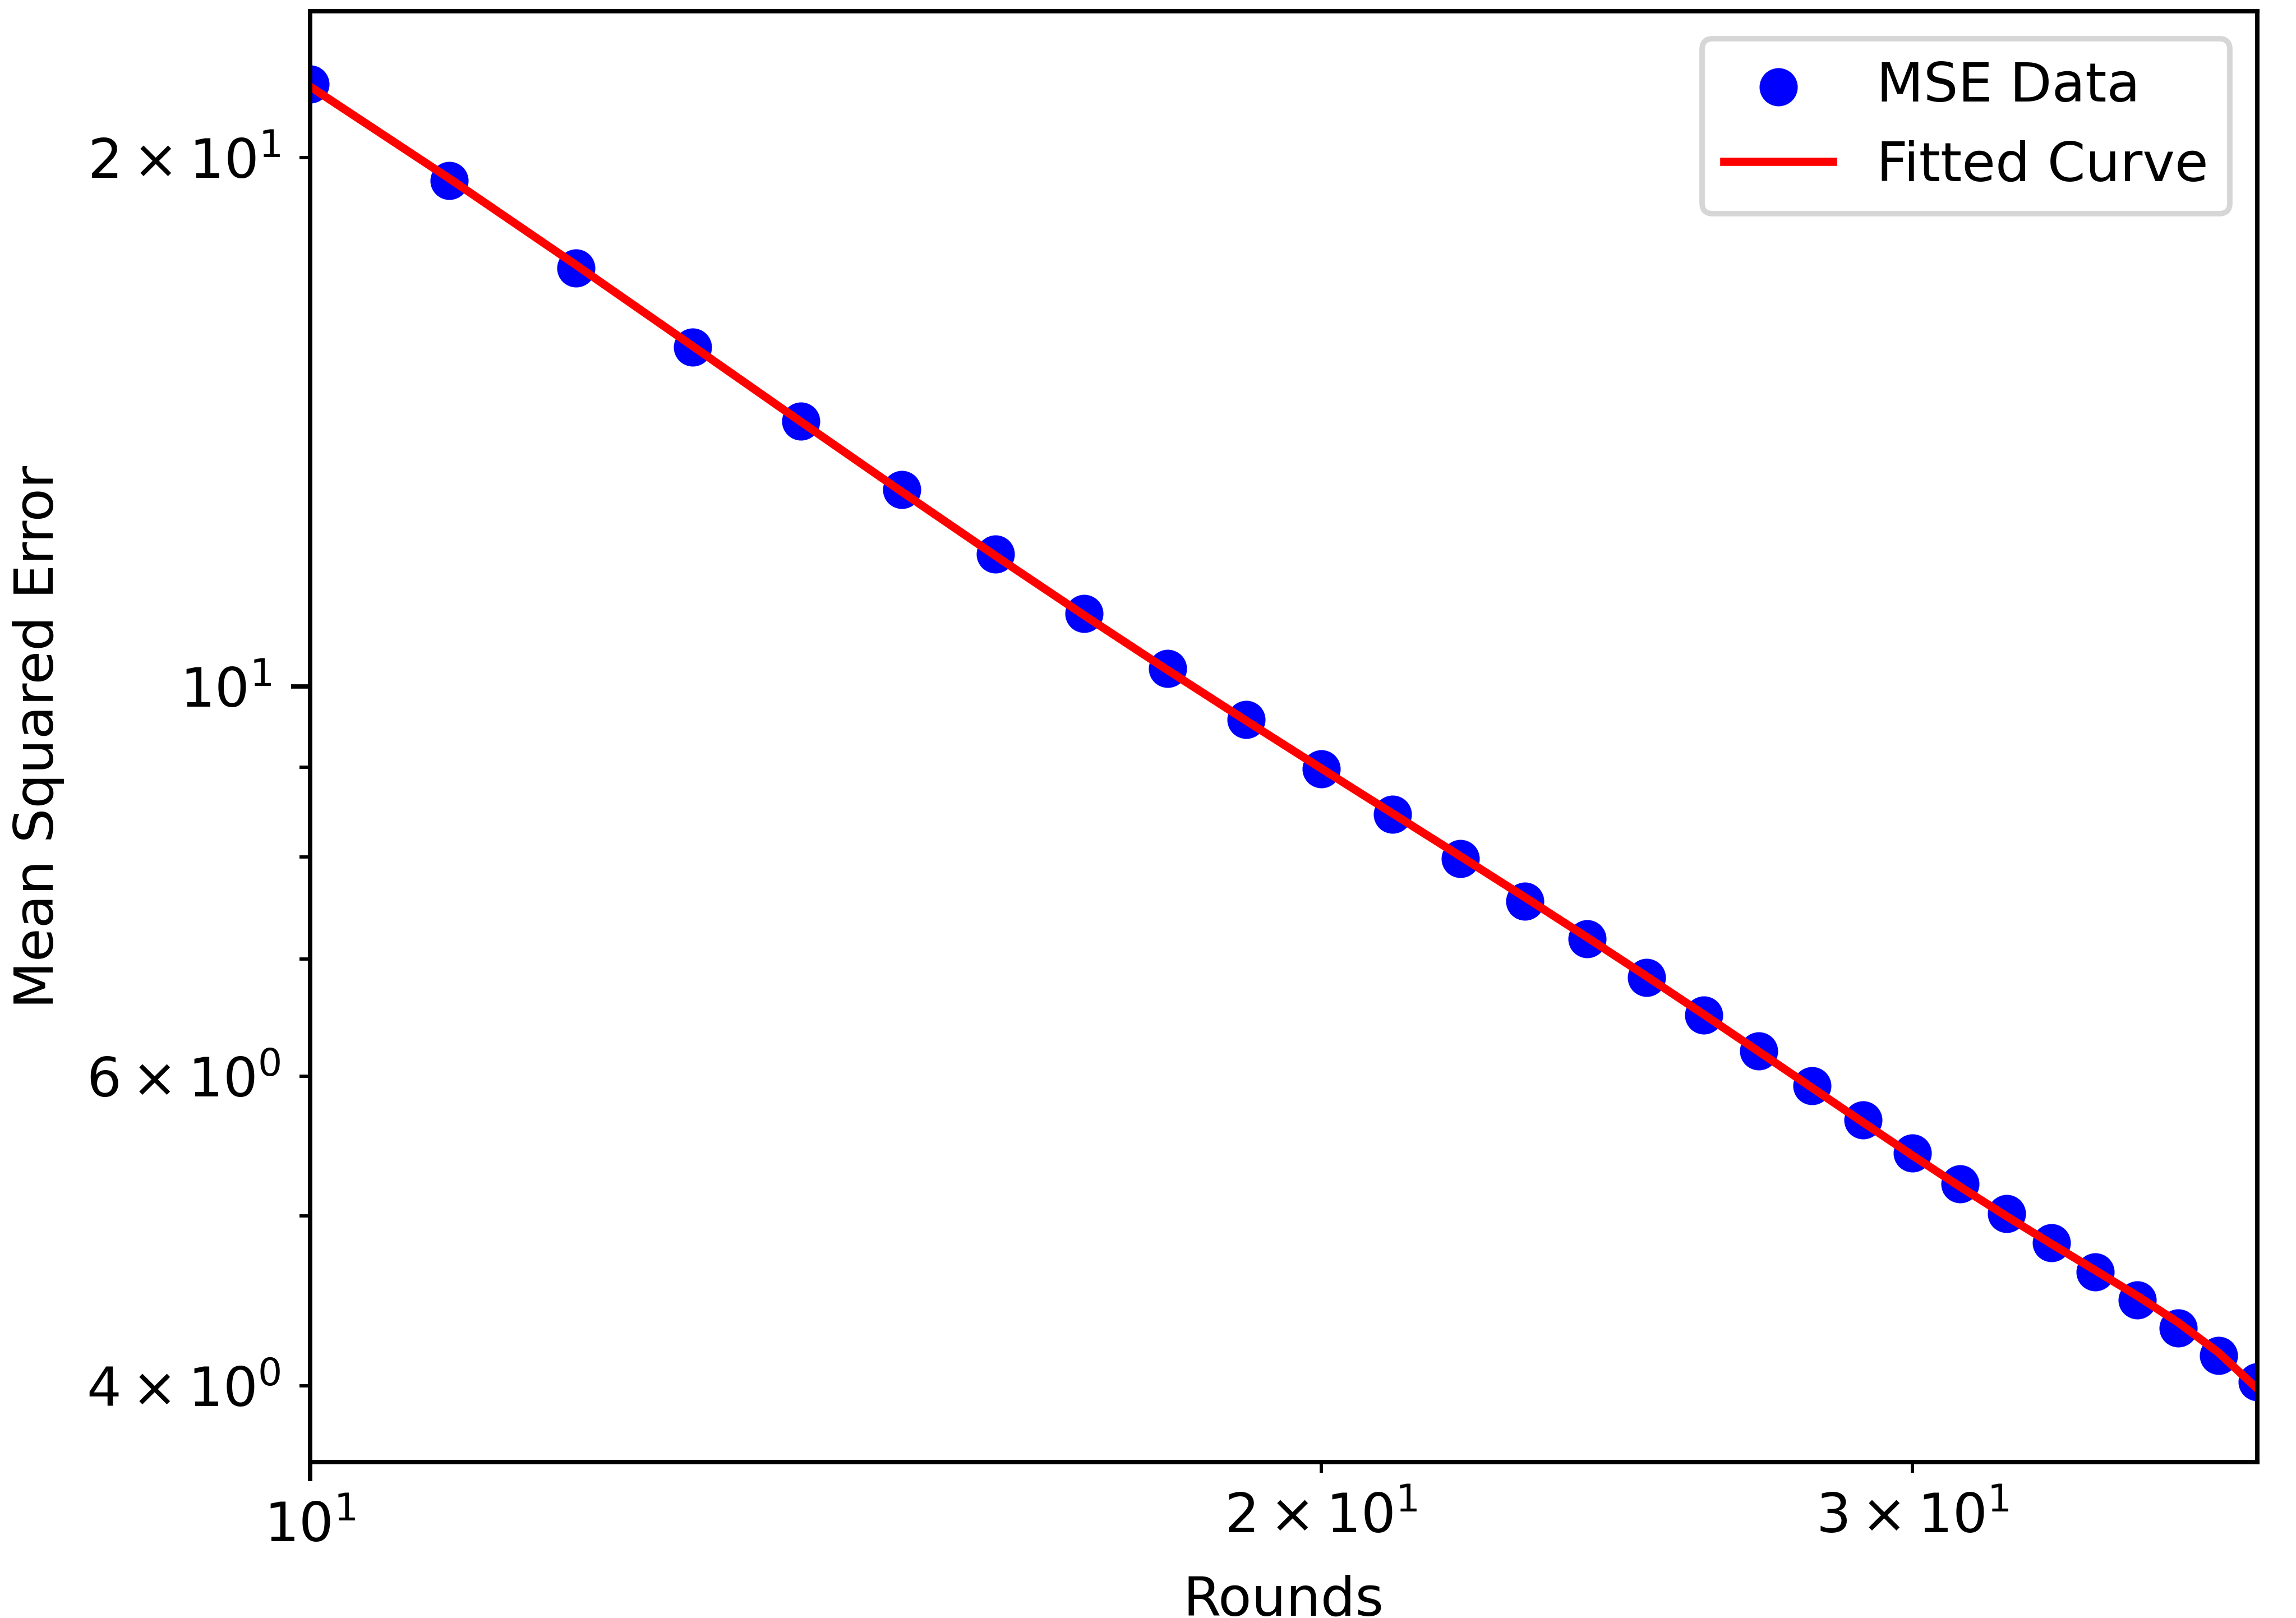
\includegraphics[width=0.49\linewidth]{figures/Simulation_outcomes/TorusGridGraph/ATPPS/ATPPS_modelfitting_rounds_38_model_2.png}}
    \hfil
        \subfloat[]{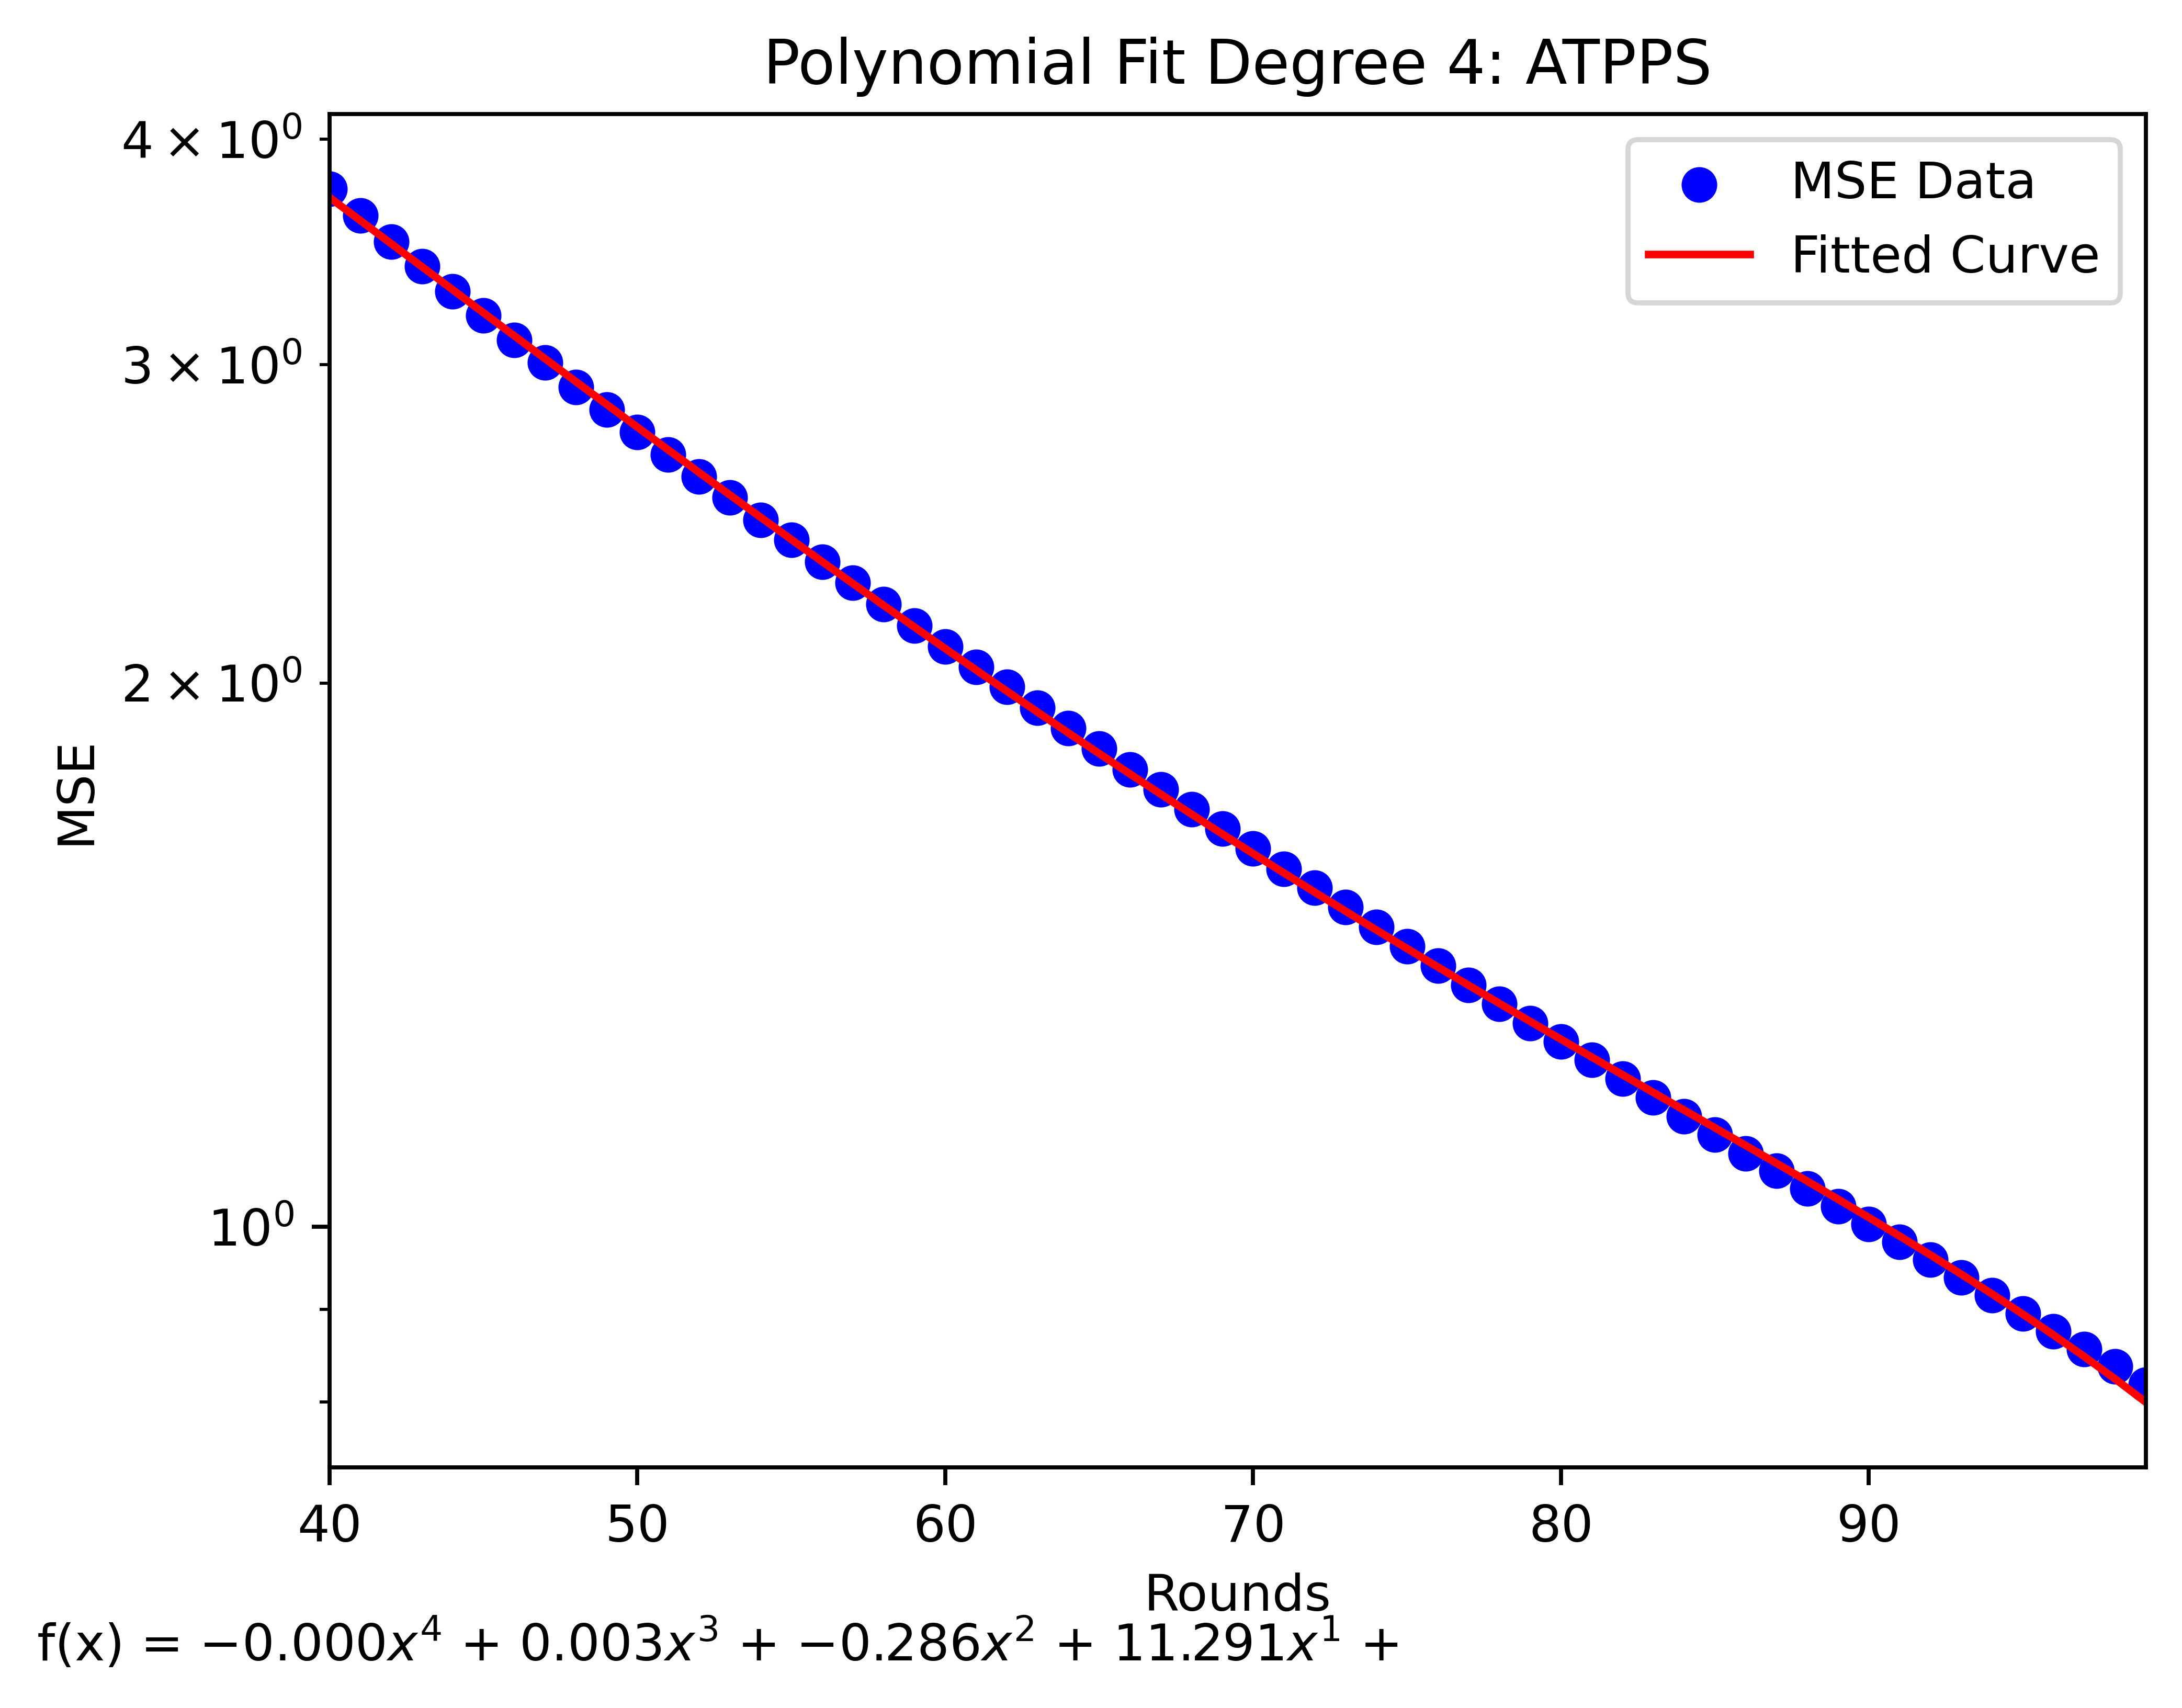
\includegraphics[width=0.49\linewidth]{figures/Simulation_outcomes/TorusGridGraph/ATPPS/ATPPS_modelfitting_rounds_99_model_2.png}}
    \caption{Torus Grid - polynomial regression fit: ATPPS; rounds 10-39 and 40-100}
        \label{fig:atppstorusModelFit}
\end{figure}
 \begin{figure}
     \centering
     \scalebox{0.8}{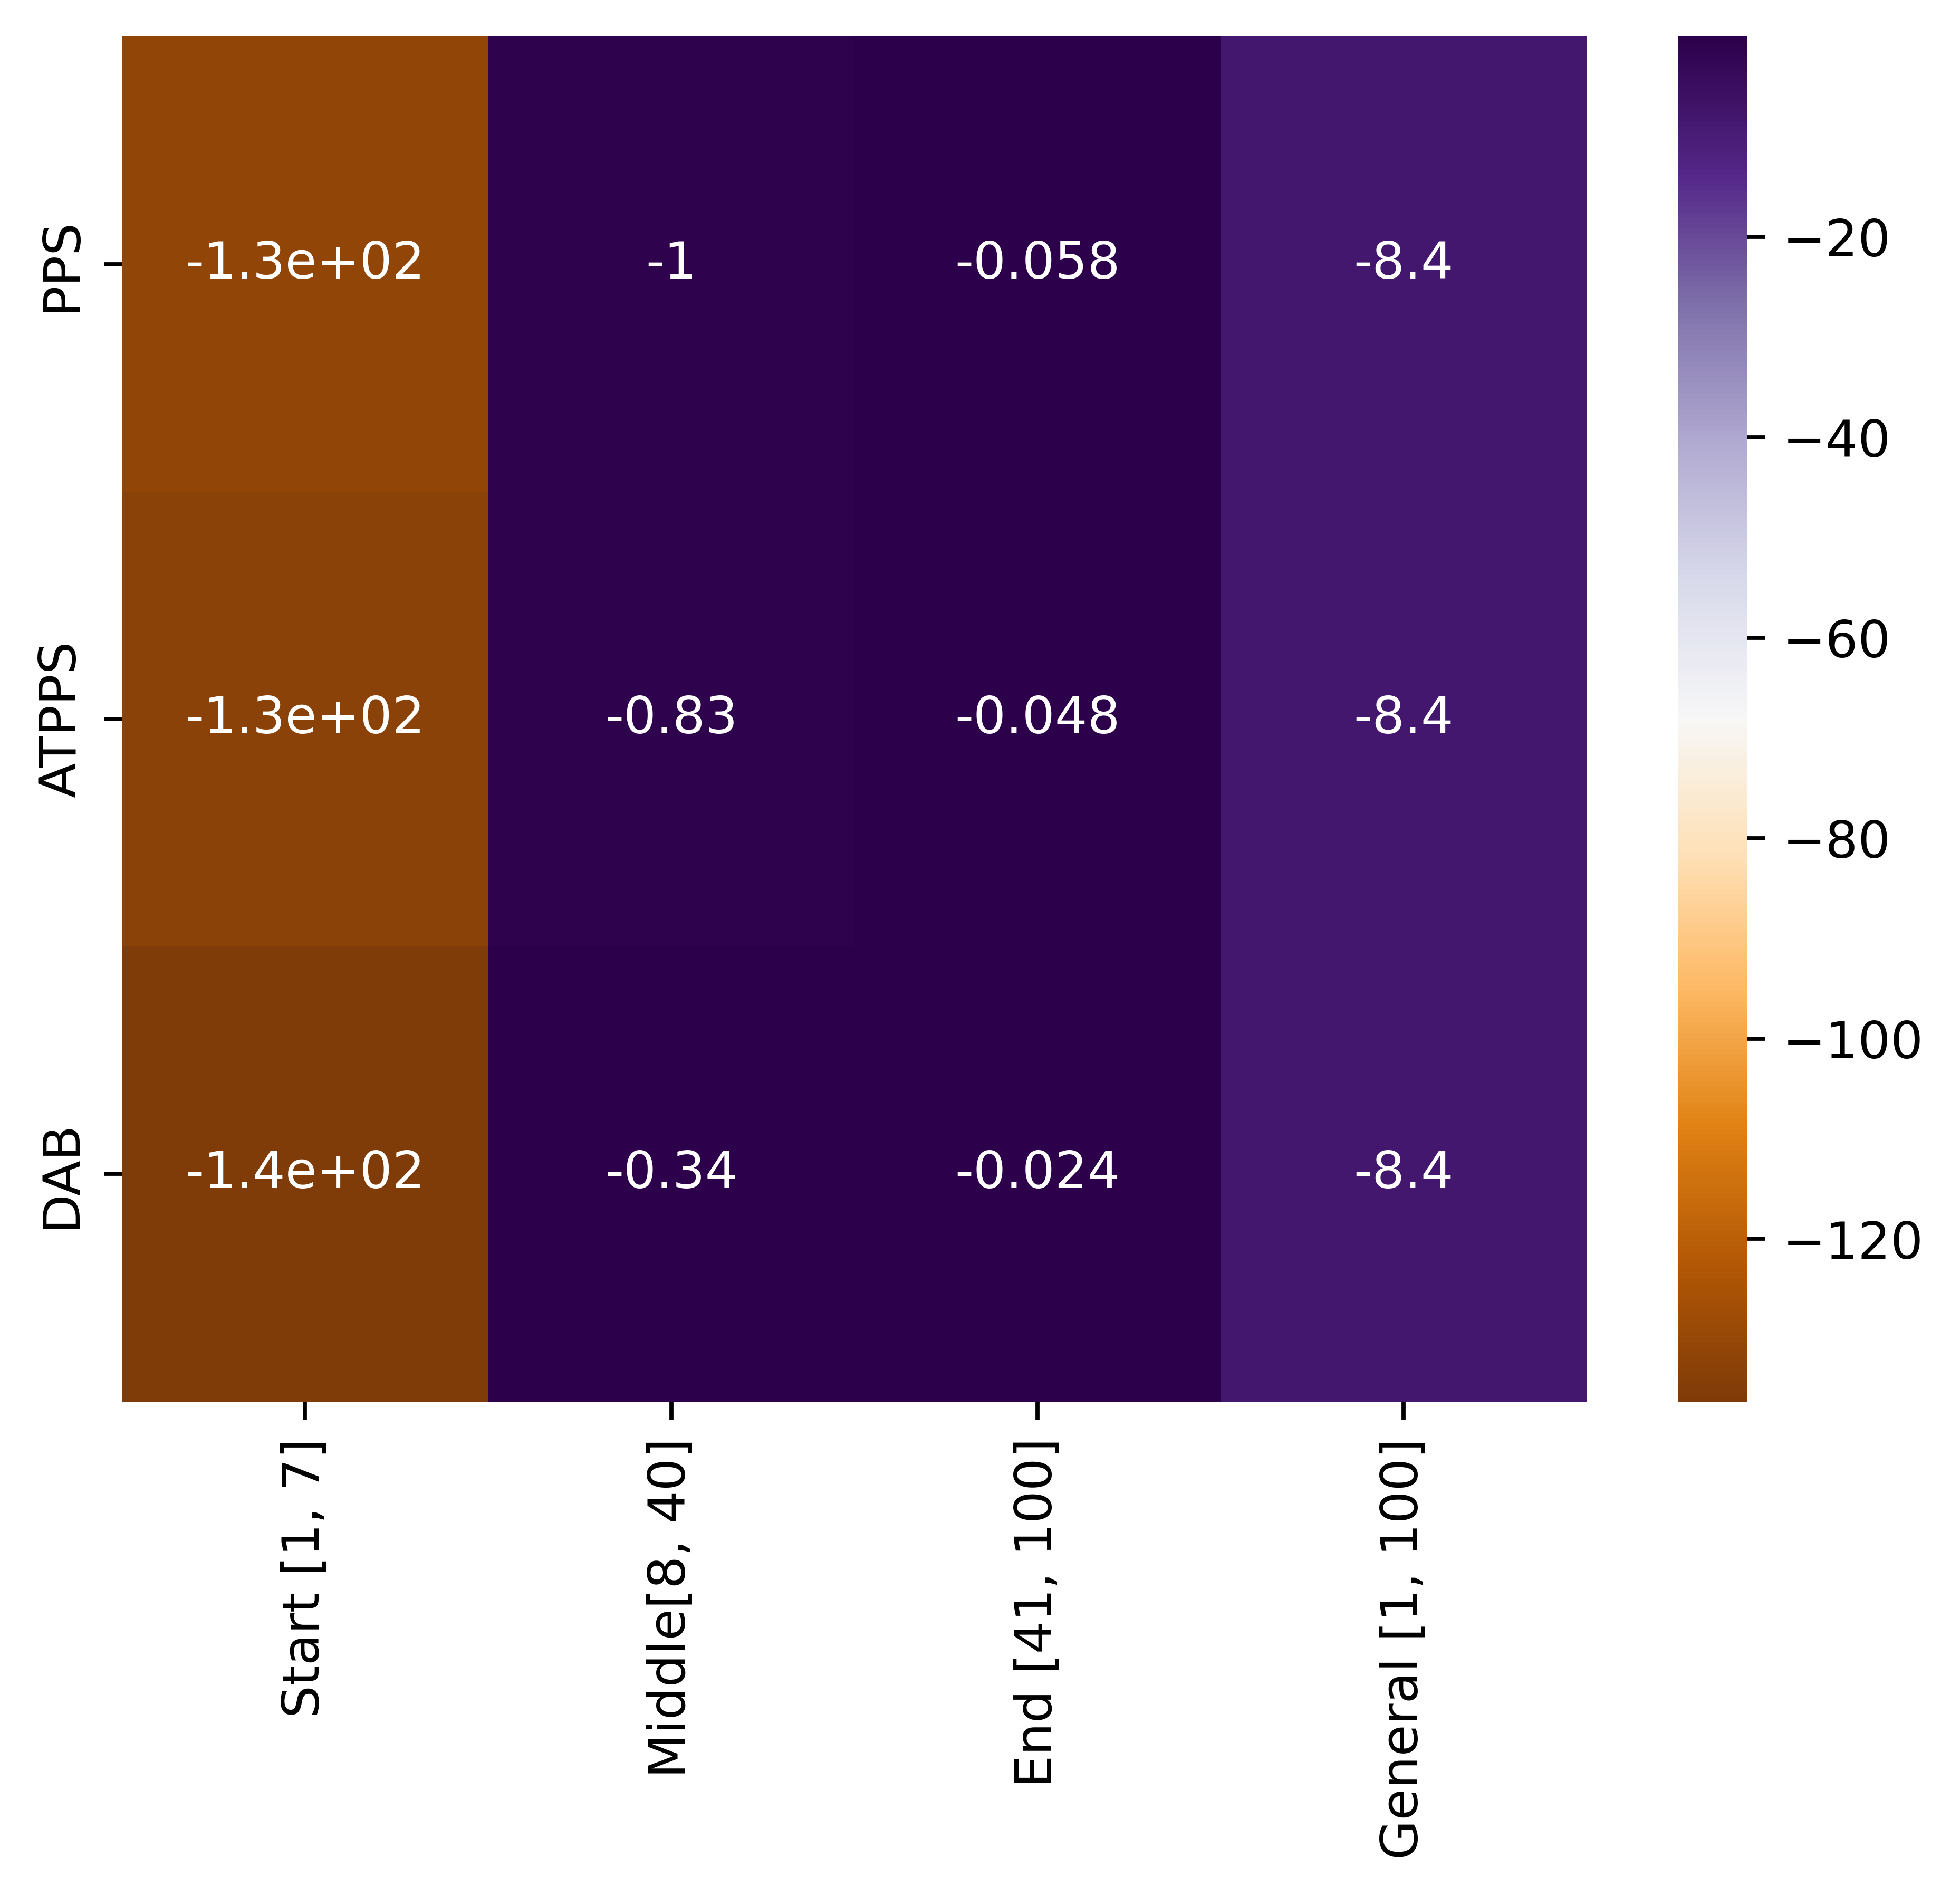
\includegraphics{figures/Simulation_outcomes/TorusGridGraph/DAB_vs_PPS_vs_ATPPS_slopesheatmap_100rounds.png}}
     \caption{Torus Grid: heat map of slopes per region}
     \label{fig:torusgraphslopes}
 \end{figure}

 \section{Lollipop Graph}\label{sec:lollipopgraph}
\subsection{(512, 512) Lollipop Graph}
Figure \ref{fig:lollipopgraphMSEperRoundLogLog} shows the three curves of the load balancing algorithms. The ATPPS slightly outperforms the PPS. The DAB lacks to perform as good as the other two load balancing algorithms in reducing the error. The superior performance of PPS and ATPPS compared to DAB in the Lollipop graph can be explained by the structure of the graph and the fundamental differences in how these algorithms operate. The clique region consists of high connectivity and enables rapid local balancing for the  Push-Pull Sum based algorithms. While the path region consists of limited connectivity and slows down information propagation and balancing for the Push-Pull Sum based algorithms and favors the deterministic algorithm DAB. The initial discrepancy in the first 10 rounds is due to the potentialy fast decrease of error for the PPS in cliques. The DAB struggles to perform good for cliques as observed in section \ref{sec:completeGraph}. DAB performs rather well in the Path graph which in theory is similar to the Ring graph without the edge connecting the first and last nodes as described in section \ref{sec:ringgraph}. It prioritizes nodes with the least load, which can lead to inefficient propagation along the clique. Load imbalances in the clique region take longer to converge because DAB does not exploit the random spreading mechanism of Push-Pull Sum based algorithms. In the initial phase PPS rapidly reduces the MSE, demonstrating strong initial convergence. The Push-Pull Sum based algorithms achieve a steep downwards slope with value -130 between rounds 1 to 7, while the DAB reaches nearly half of it with value -67 (figure \ref{fig:lollipopslopes}) In the mid-to-late phase the slope flattens for both of the Push-Pull Sum based algorithms, indicating slower convergence this is also indicated by the slopes droping to as low as $-0.12$ to $\sim-0.9$. In this phase, the path section of the Lollipop graph dominates the residual imbalances. The ATPPS achieves nearly identical behavior to the PPS in the early rounds, as it starts with similar strategies where the threshold is relatively easy surpassed as the load differences in the network are still very high. ATPPS outperforms the PPS slightly in the later rounds due to its ability to dynamically adjust its balancing strategy based on the current state of load imbalances. This allows it to better address residual imbalances in the path section of the Lollipop graph as showcased in section \ref{sec:ringgraph}.

The DAB model fit follows the equation: $MSE_r=-5.89\times10^{-5}r^{3}+0.03r^{2}-5.68r+459.42$ (figure \ref{fig:dablollipopgraphModelFit}), which is a 4-th degree polynomial equation. The PPS and ATPPS are a bit more complex and expressed by a polynomial equation of degree 5. The PPS model fit follows the equation: $MSE_r=8.44\times 10^{-7}r^{4}-2.52\times 10^{-4}r^{3}-0.03r^{2}-1.64r+56.68$ (figure \ref{fig:ppslollipopgraphModelFit}) and the ATPPS model fit follows the equation: $MSE_r=8.69 \times 10^{-7}r^{4}-2.56 \times 10^{-4}r^{3}+0.03r^{2}-1.62r+54.48$ (figure \ref{fig:atppslollipopgraphModelFit}).

\begin{figure}[]
    \centering
    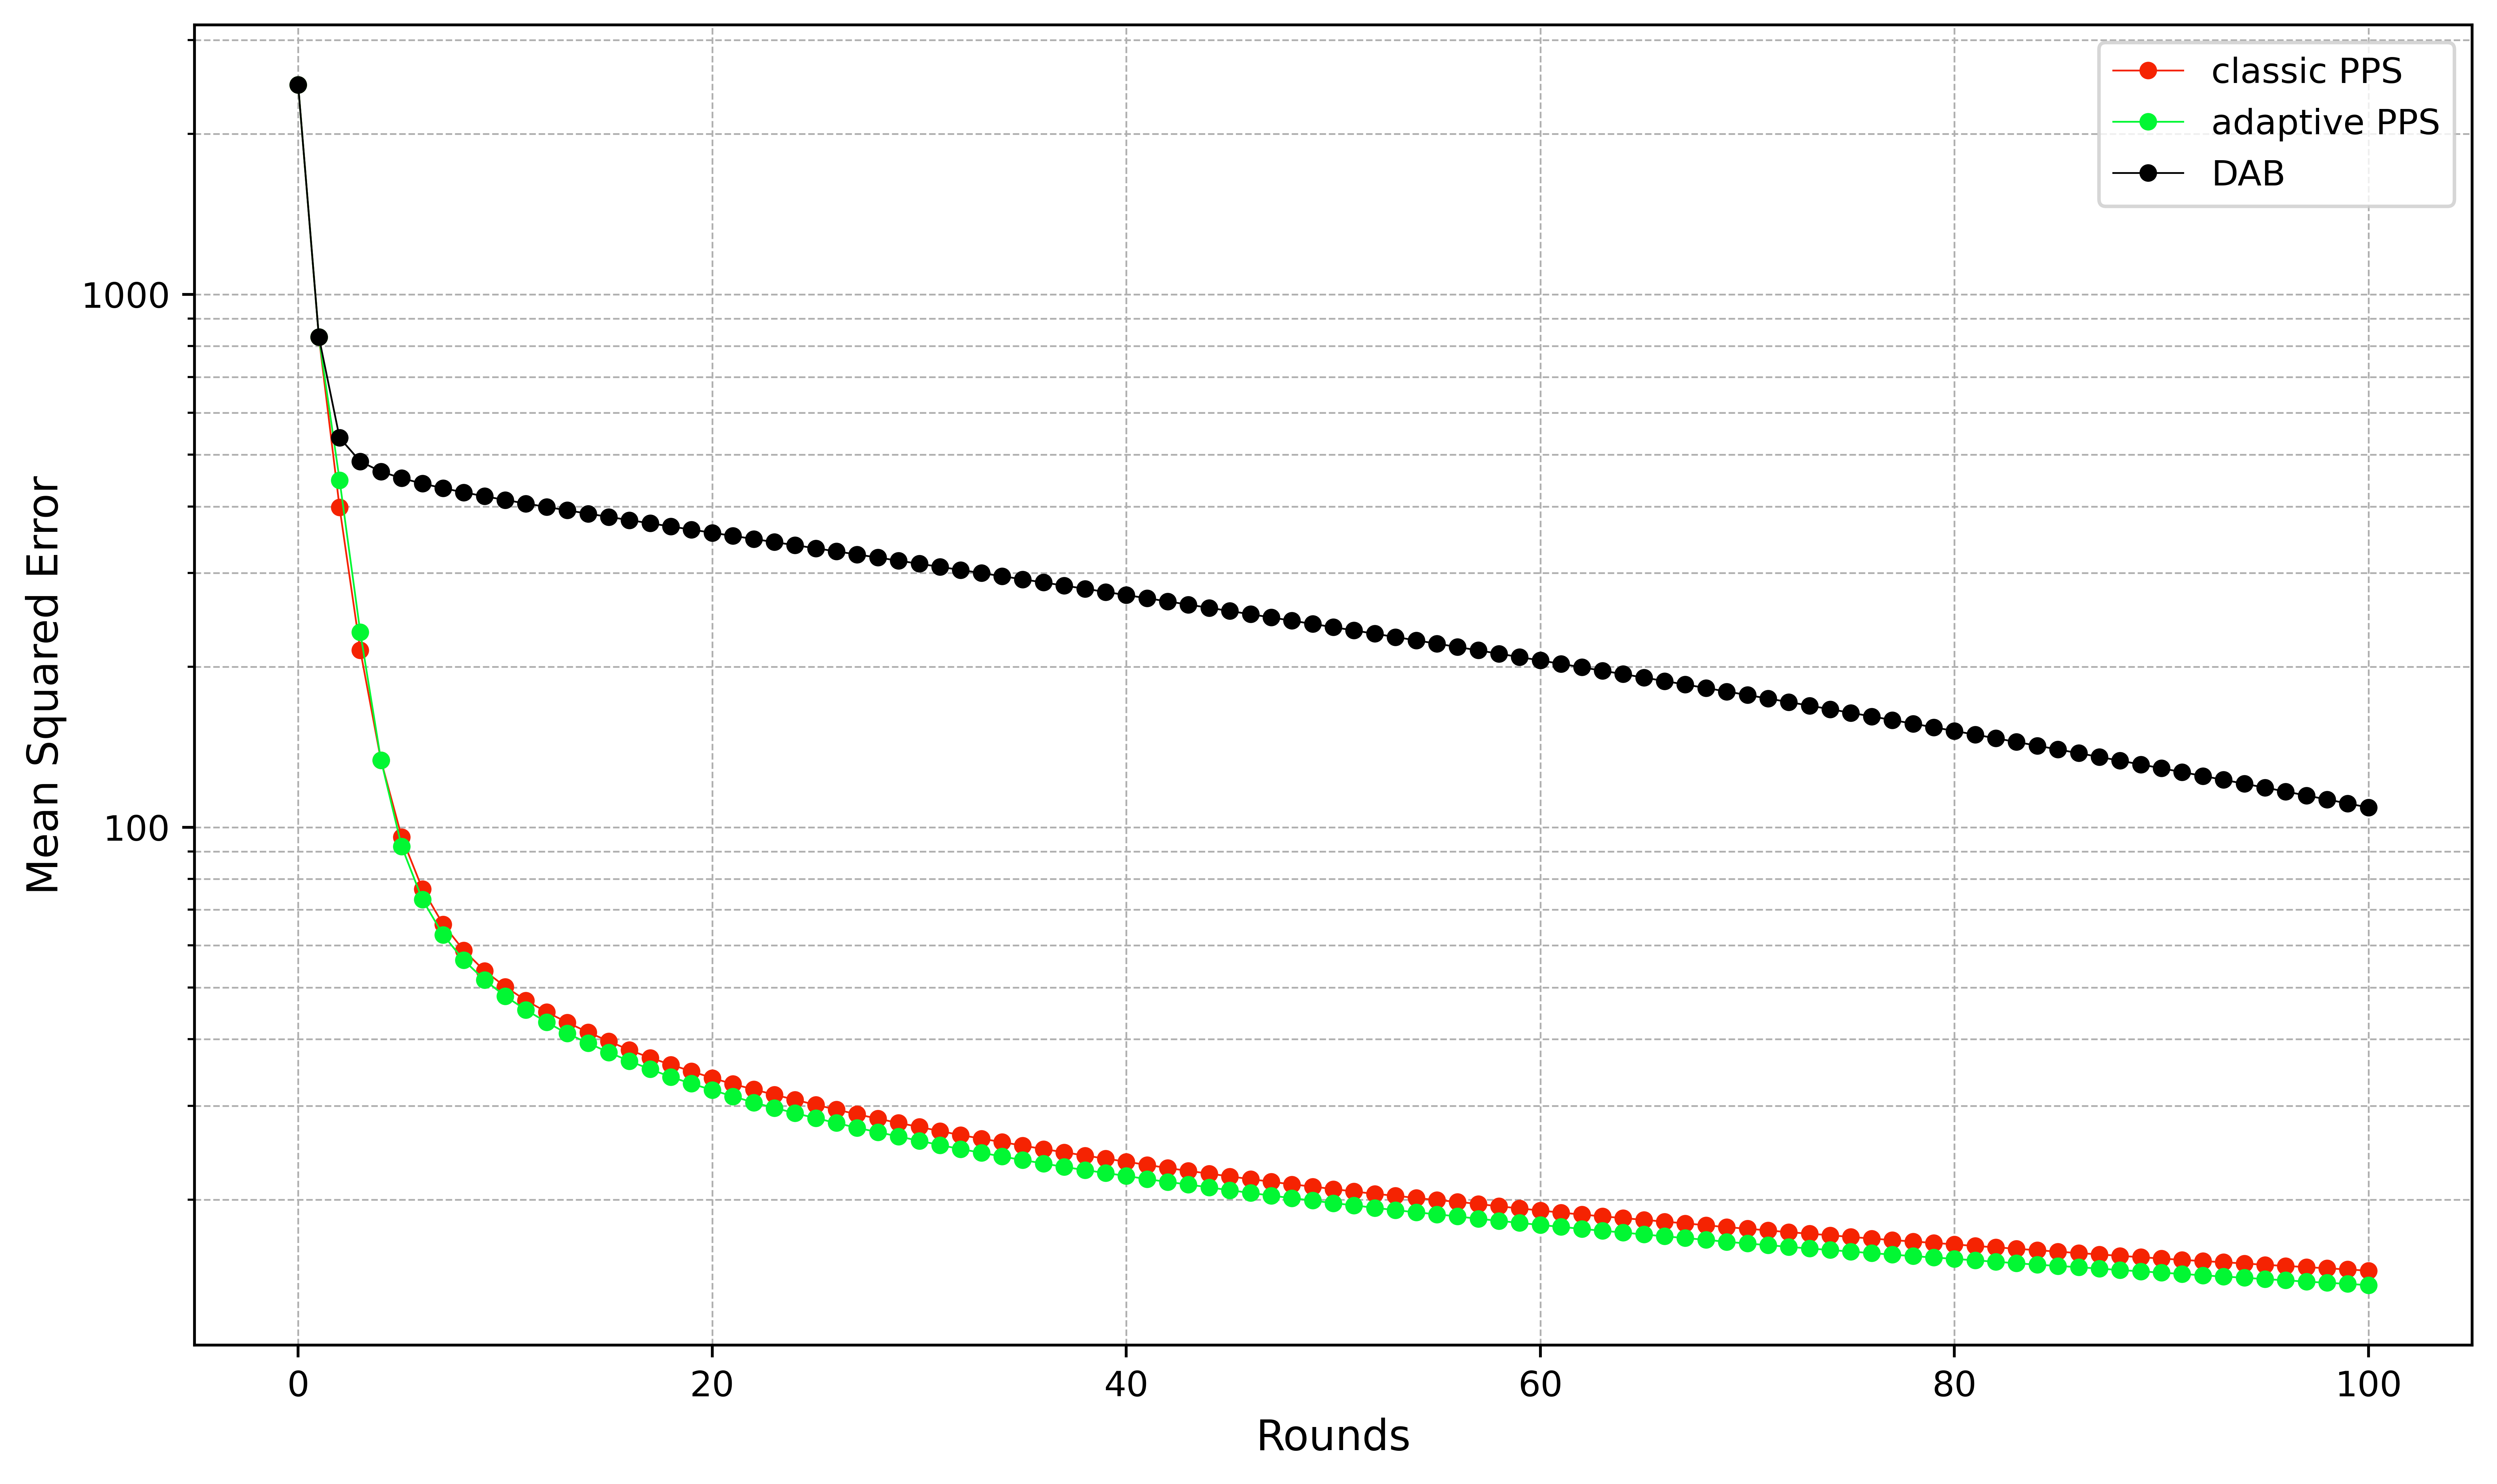
\includegraphics[width=\linewidth]{figures/Simulation_outcomes/LollipopGraph/512_512/DAB_vs_PPS_LG_r100_n1024_averaged_log.png}
    \caption{(512, 512)-Lollipop graph: mean squared error per rounds (log-linear)}
    \label{fig:lollipopgraphMSEperRoundLogLog}
\end{figure}

\begin{figure}[]
    \centering
    \scalebox{0.8}{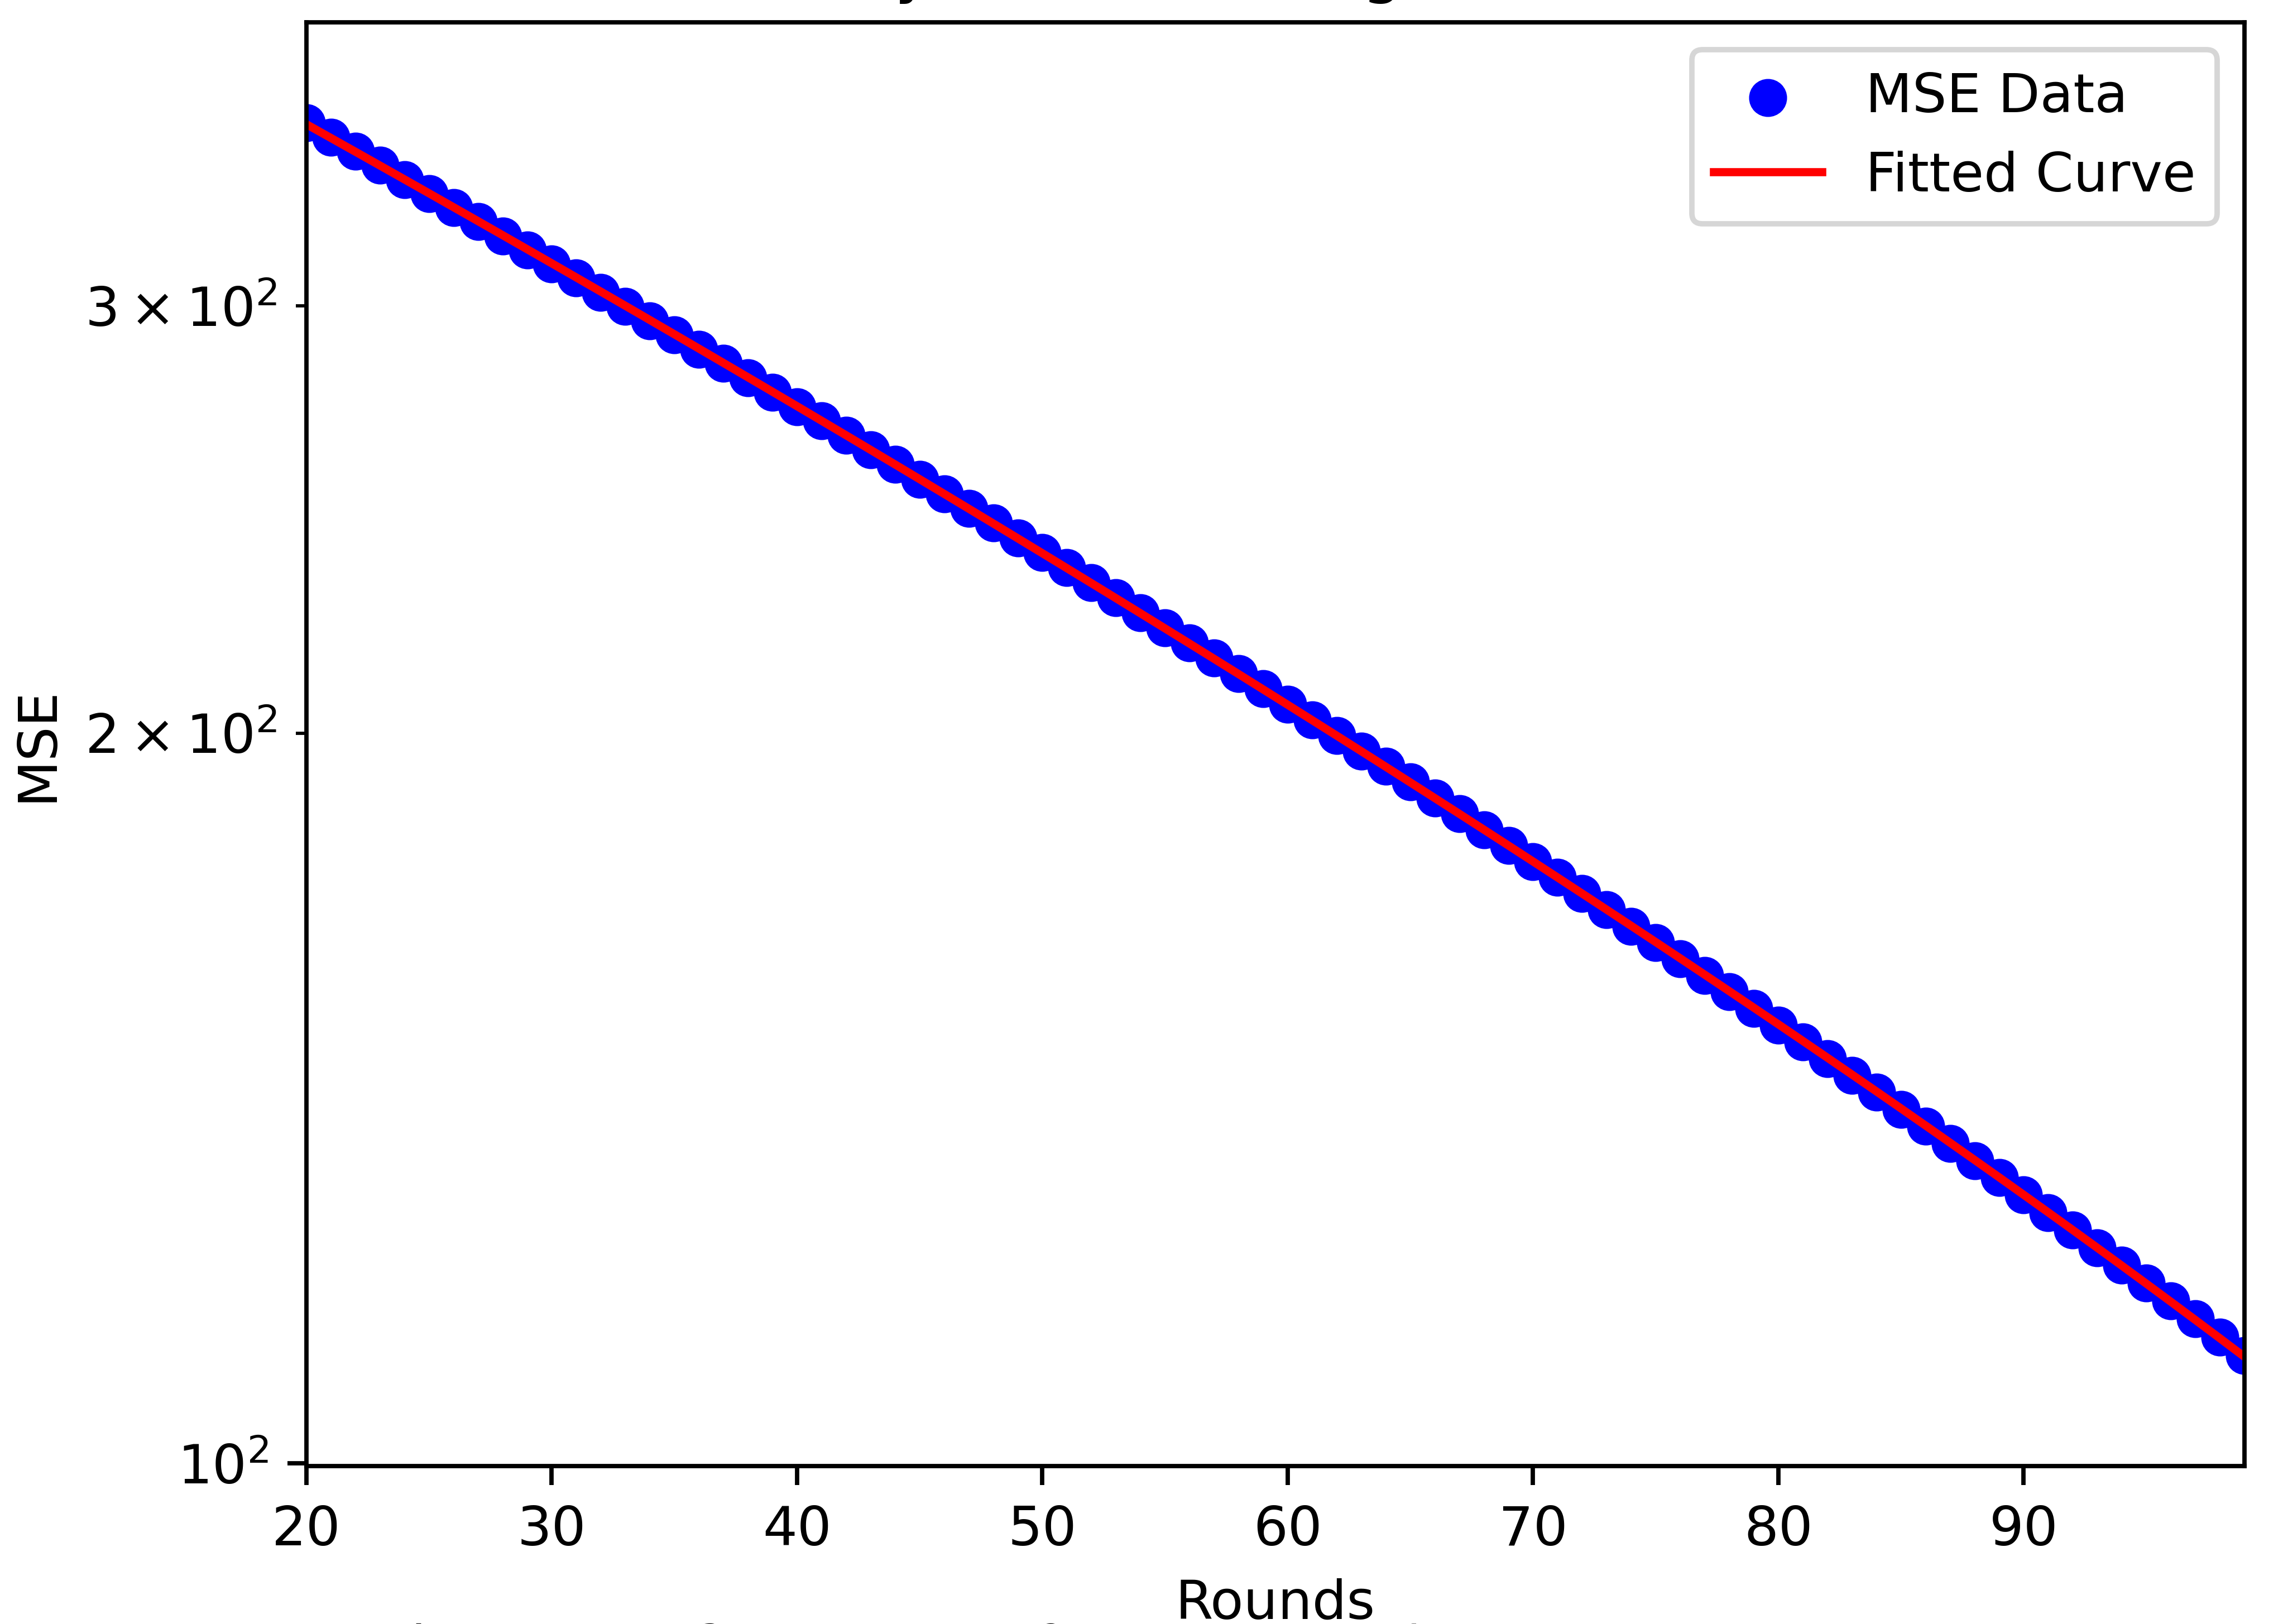
\includegraphics{figures/Simulation_outcomes/LollipopGraph/512_512/DAB/DAB_modelfitting_rounds_99_model_2.png}}
    \caption{(512, 512)-Lollipop graph - polynomial regression fit: DAB}
    \label{fig:dablollipopgraphModelFit}
\end{figure}

\begin{figure}[]
    \centering
    \scalebox{0.8}{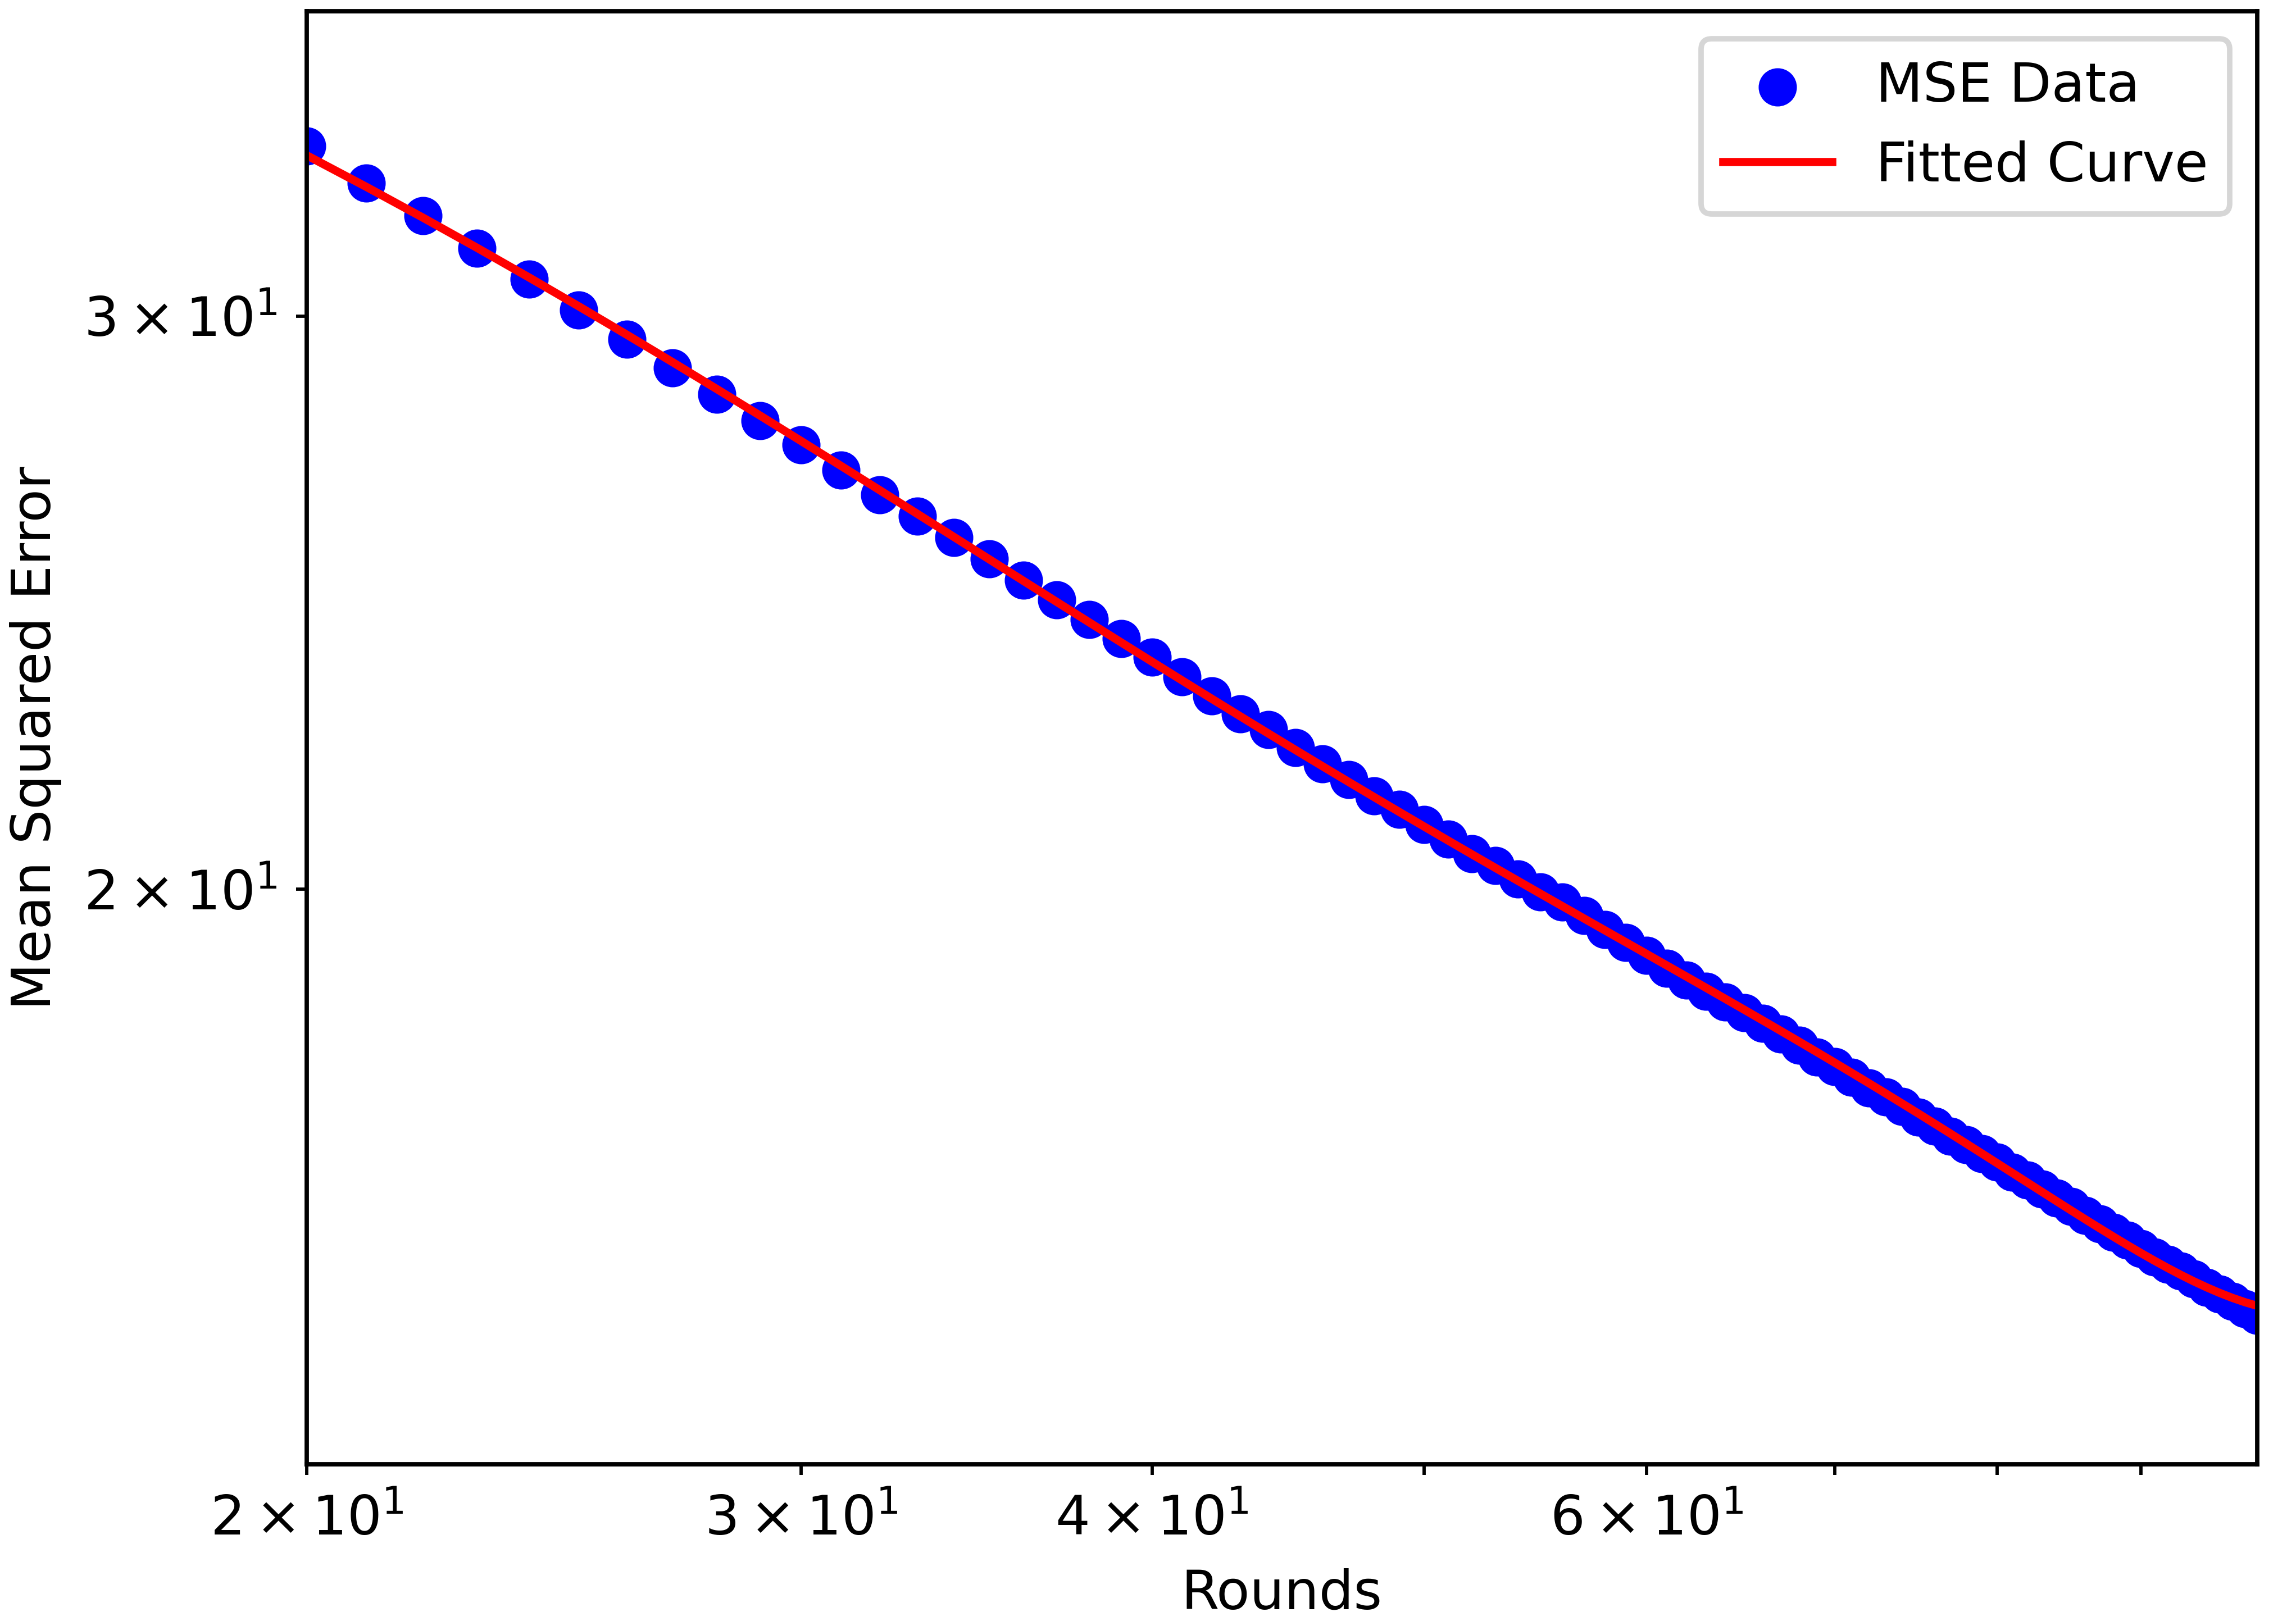
\includegraphics{figures/Simulation_outcomes/LollipopGraph/512_512/PPS/PPS_modelfitting_rounds_99_model_2.png}}
    \caption{(512, 512)-Lollipop graph - polynomial regression fit: PPS}
    \label{fig:ppslollipopgraphModelFit}
\end{figure}

\begin{figure}[]
    \centering
    \scalebox{0.8}{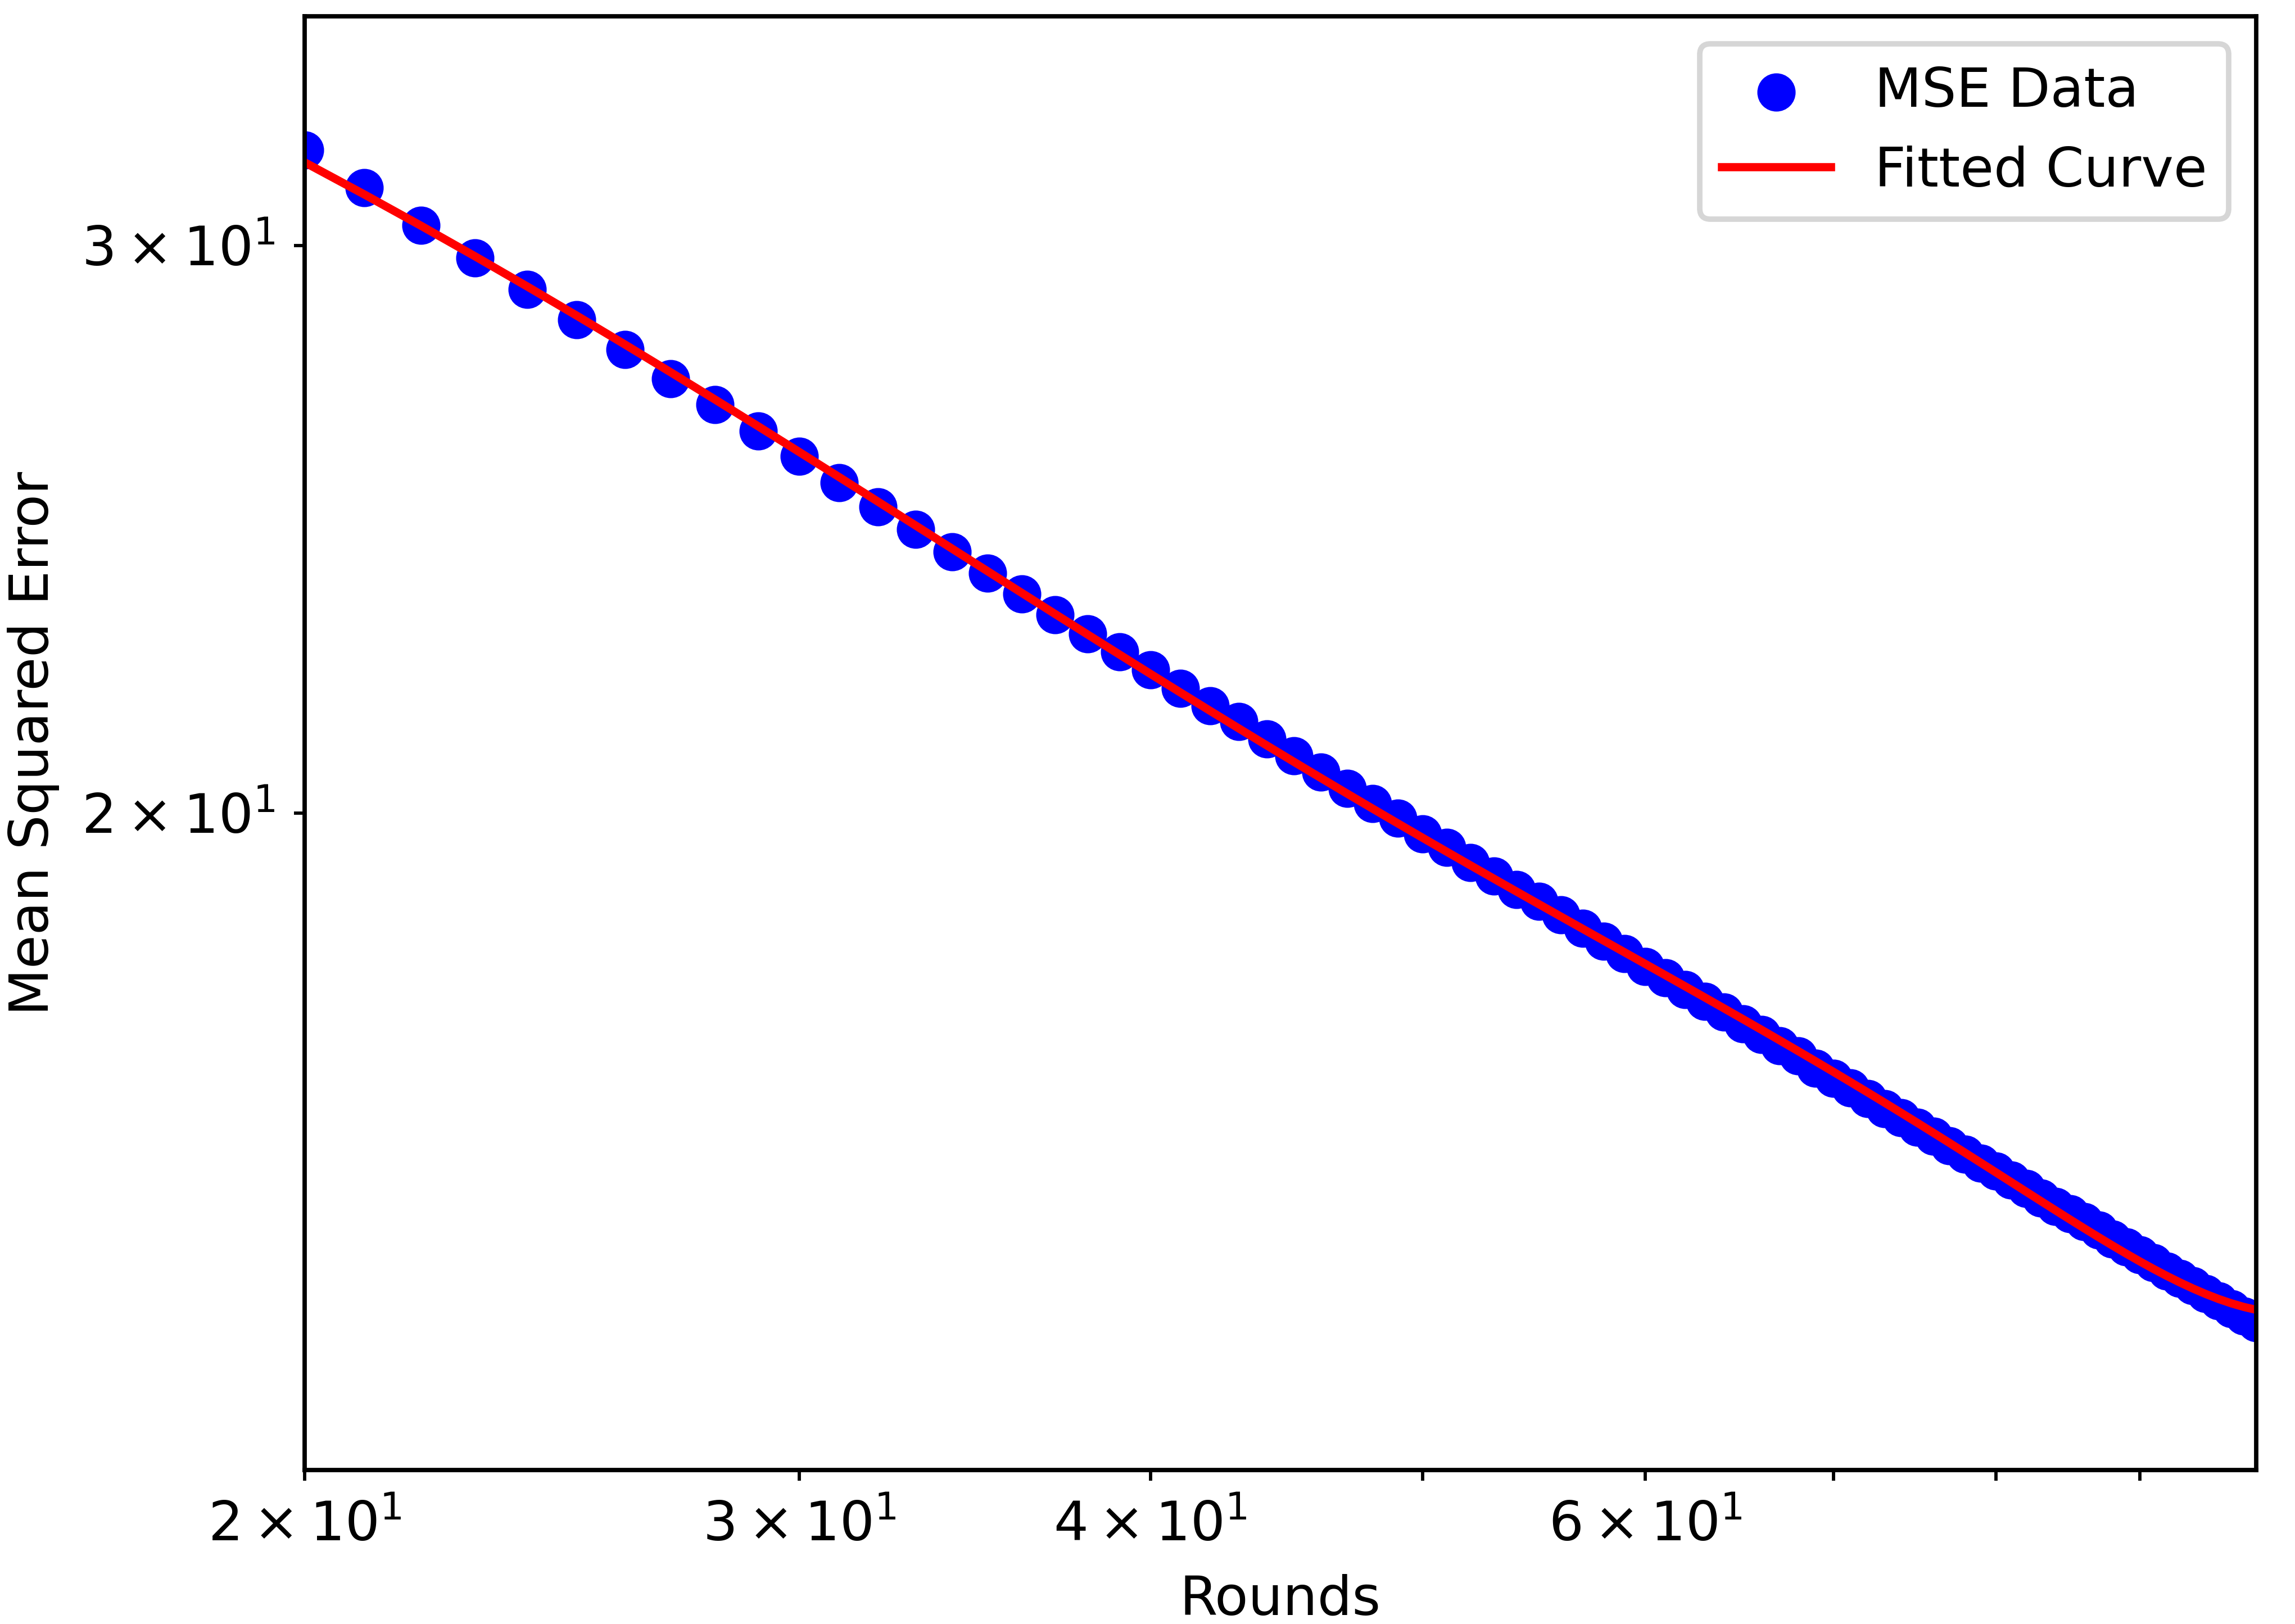
\includegraphics{figures/Simulation_outcomes/LollipopGraph/512_512/ATPPS/ATPPS_modelfitting_rounds_99_model_2.png}}
    \caption{(512, 512)-Lollipop graph - polynomial regression fit: ATPPS}
    \label{fig:atppslollipopgraphModelFit}
\end{figure}

\begin{figure}
    \centering
    \scalebox{0.8}{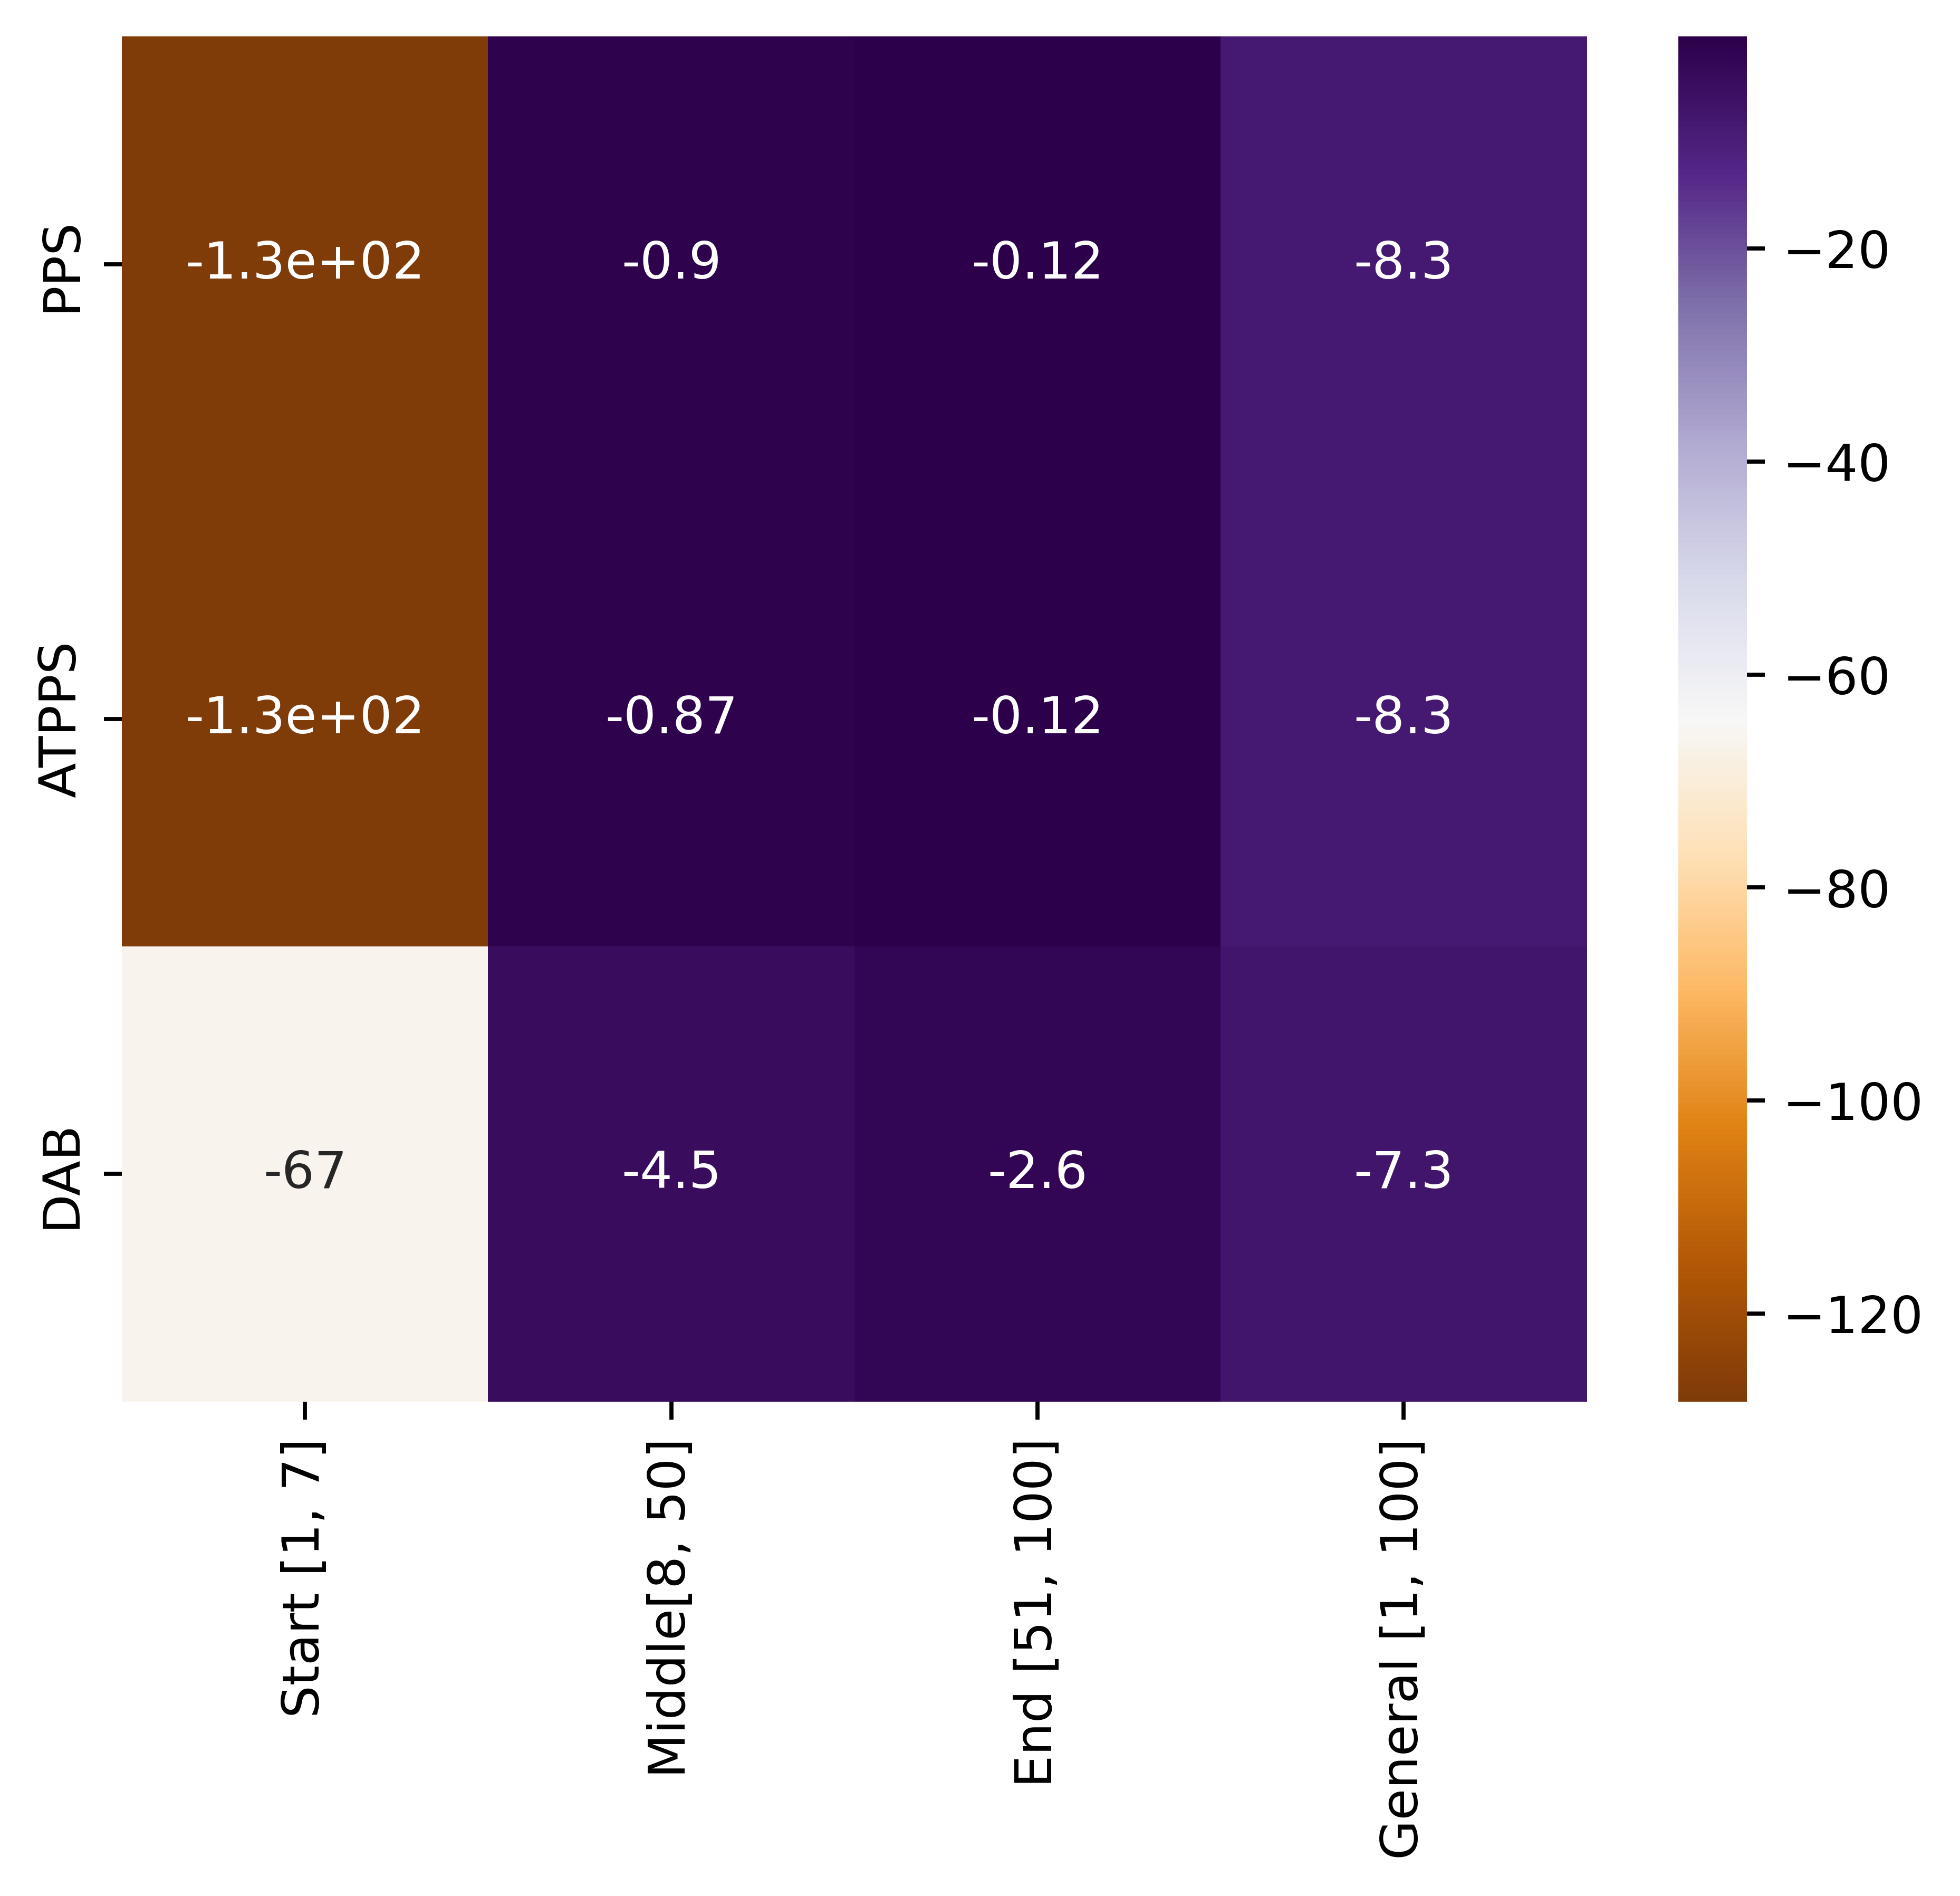
\includegraphics{figures/Simulation_outcomes/LollipopGraph/512_512/DAB_vs_PPS_vs_ATPPS_slopesheatmap_100rounds.png}}
    \caption{Lollipop graph: heat map of slopes per region}
    \label{fig:lollipopslopes}
\end{figure}

To see the impact of the pathsize and cliquesize on the simulation results respectively, the simulations are conducted with less nodes assigned to the clique in subsection \ref{subsec:128_896lollipop}. The network sizes remains the same. The nodes assigned to the cliques are cut to 128 which is one fourth of the previous value of 512. Thus 896 nodes are assigned to the path size. And similarly the simulations are conducted with less nodes assigned to the path in subsection \ref{subsec:896_128lollipop}.  

\subsection{(128, 896) Lollipop Graph}\label{subsec:128_896lollipop}
In the initial region, the first 7 rounds, PPS and ATPPS start with a steep decrease in MSE with a slope of -86 as depicted in figure \ref{fig:128_896lollipopslopes}. DAB, on the other hand, has a slightly slower initial convergence compared to PPS showcasing a slope of -110. Compared to the slopes of the previous experiment where the path size and the clique size where equal, the convergece in the first 7 rounds improved for the DAB, achieving a steeper downwards slope. The slope in this region in the previous experiment was -68 and improved to -110. In the middle region, rounds 8 to 50, the ATPPS shows a performance close to that of the PPS where both curves maintain a consistently steep slope. In this region the DAB shows to have the steepest slope decreasing the error by -2.8 on average per round. The PPS and ATPPS already show low MSE values beforehand due to the steep decrease of error in the initial phase, thus only reduce the error by around $\sim -1.5$ per round on average. In the end region the DAB shows a slightly sharper decline in MSE compared to earlier rounds. This could be due to the longer path structure of the graph: once the majority of the load has propagated through the clique, the balancing process accelerates. Both Push-Pull Sum variants continue to outperform DAB, achieving lower MSE values in fewer rounds due to their clique-centric structure, which more effectively balances loads in the smaller clique. Interestingly the PPS and ATPPS slightly diverge between rounds 10 and 90 and finaly interesect (or nearly) in round 100.

\begin{figure}[]
    \centering
    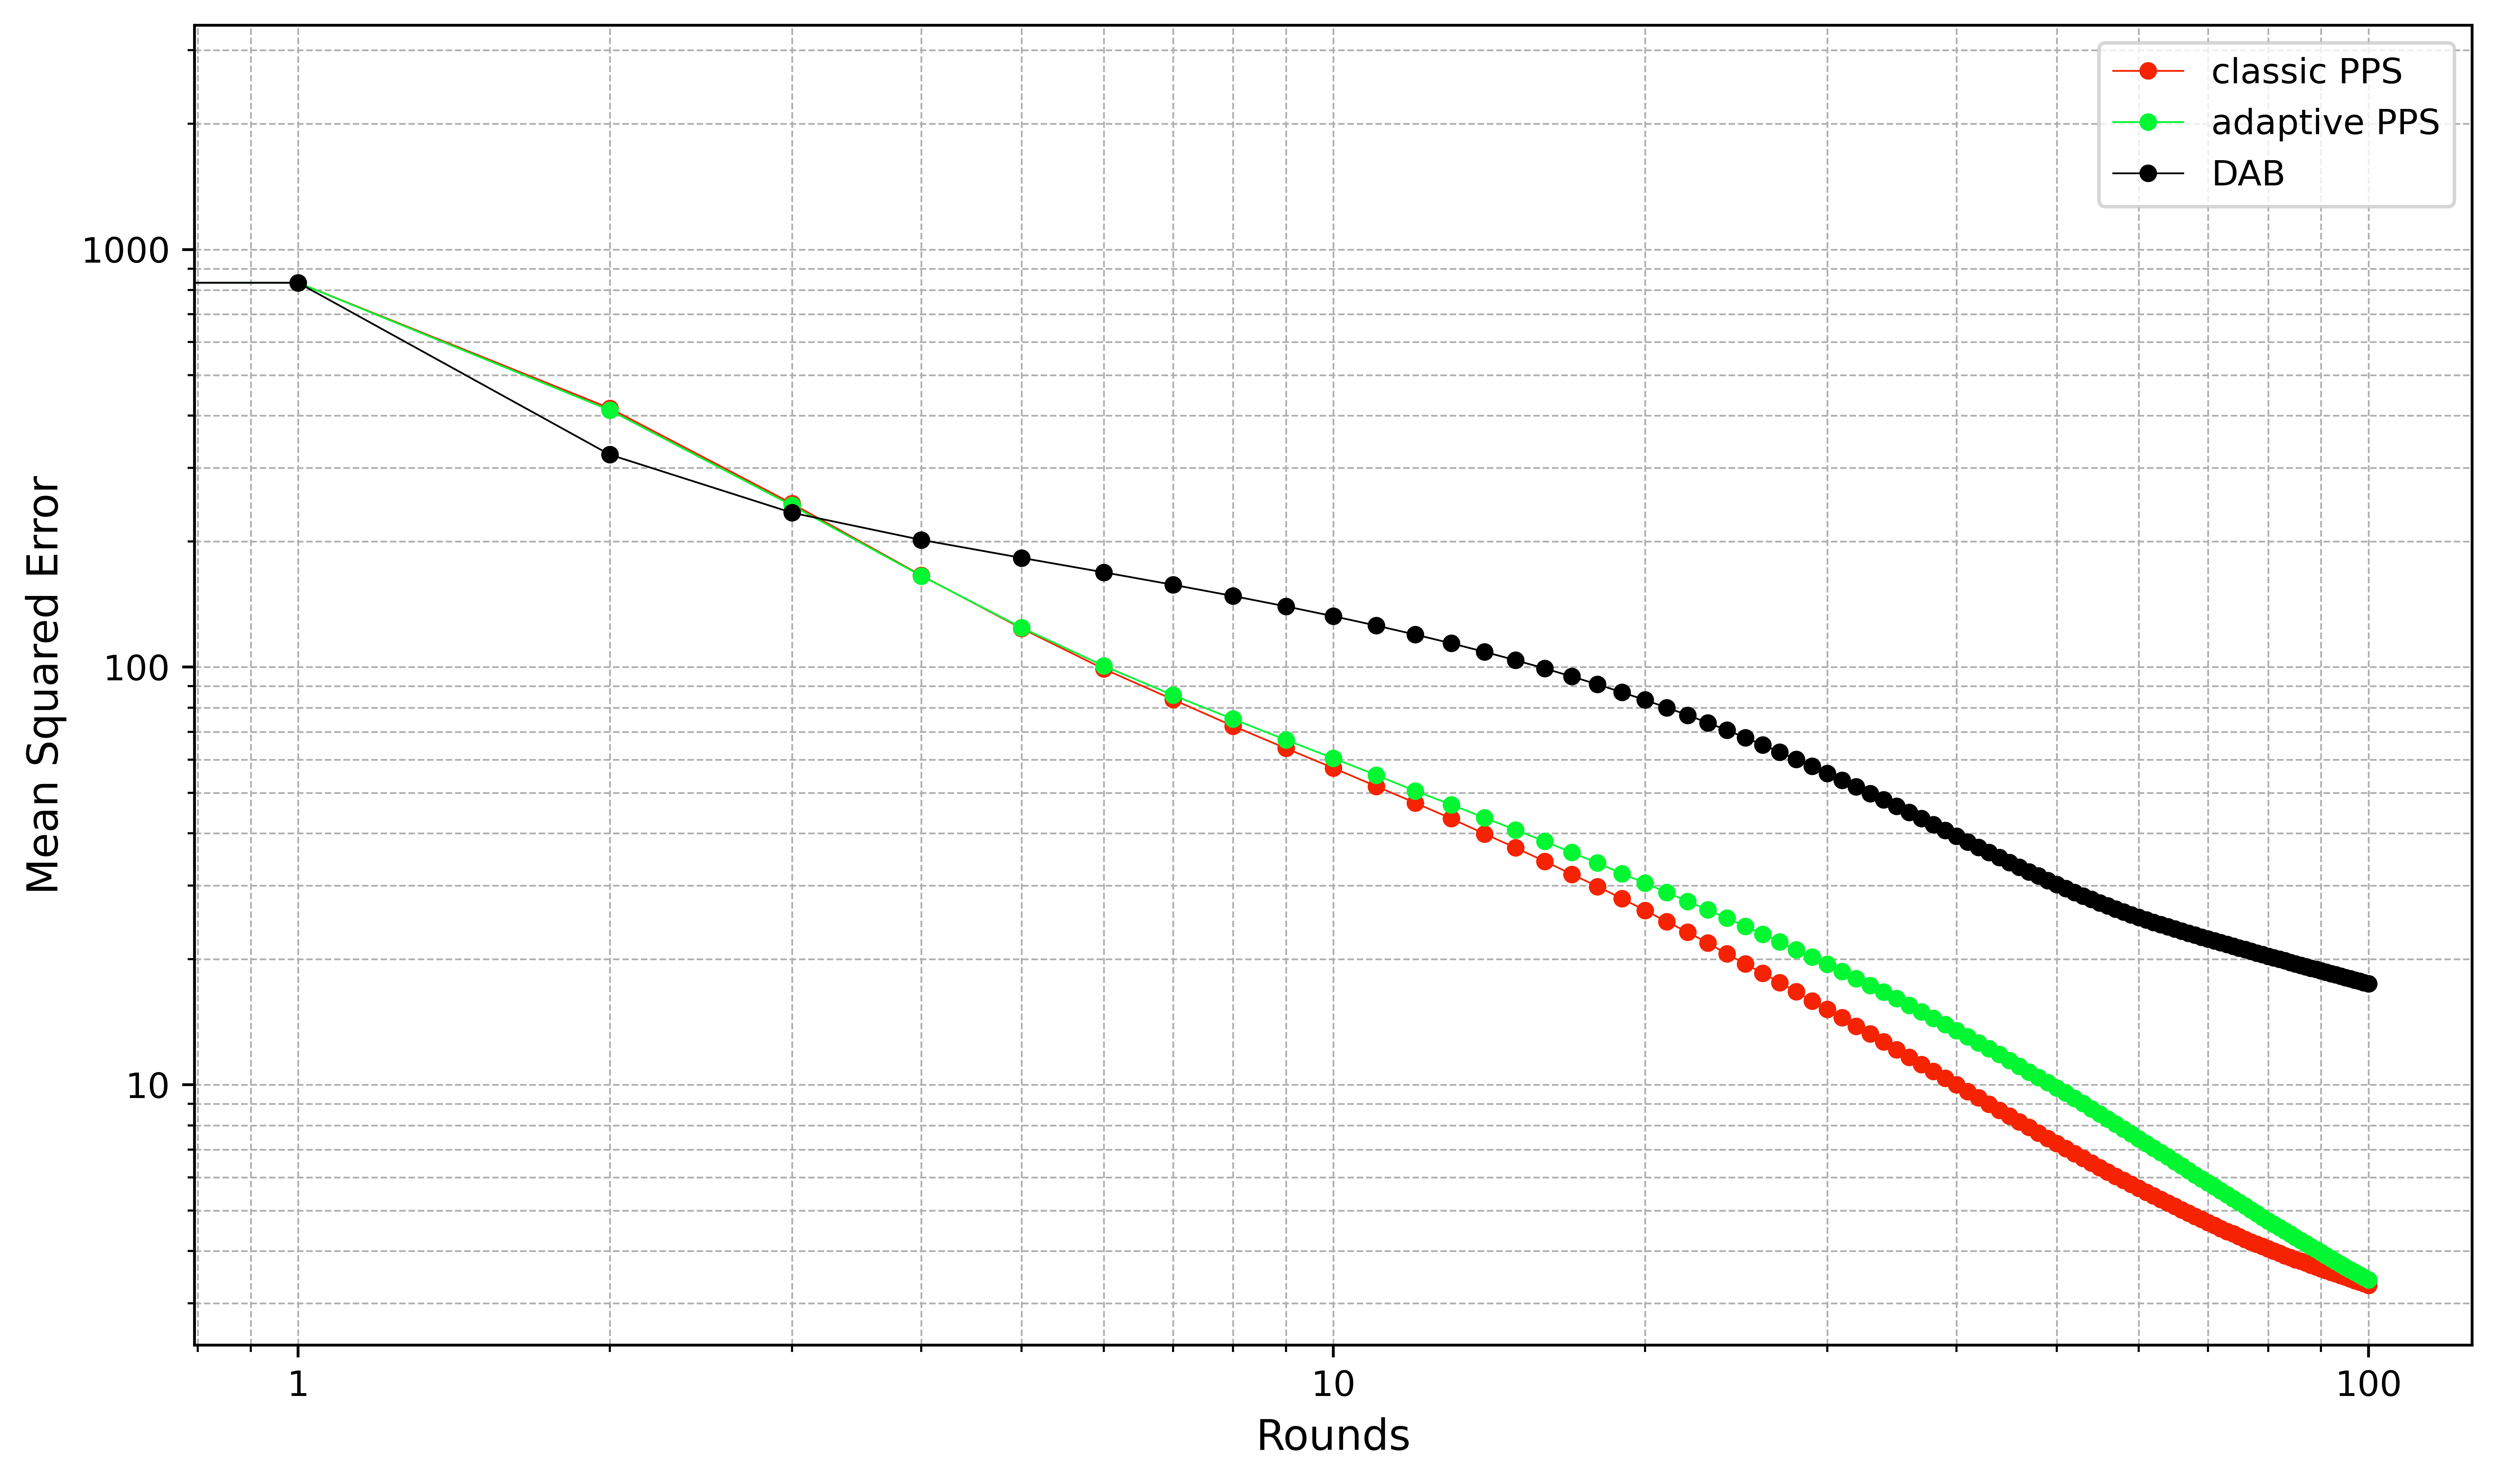
\includegraphics[width=\linewidth]{figures/Simulation_outcomes/LollipopGraph/128_896/DAB_vs_PPS_LG_r100_n1024_averaged_loglog.png}
    \caption{(128, 896)-Lollipop graph: mean squared error per rounds (log-log)}
    \label{fig:128_896lollipopgraphMSEperRoundLogLog}
\end{figure}

The MSE data of all three load balancing algorithms fit a equation of the polynomial regression model. The MSE data of the DAB and ATPPS are fitted to a polynomial of degree 4 each, while the PPS MSE data seems to be a bit more complex following a polynomial of degree 5. The fitted model of the DAB MSE data follows the equation: $MSE_r=3.46\times 10^{-6}r^{4}-1.12\times 10^{-3}r^{3}+0.14r^{2}-7.69r+190.78$ (figure \ref{fig:dab_128x896lollipopgraphModelFit}) and the one of the ATPPS follows the equation $MSE_r=1.59\times 10^{-6}r^{4}-4.74\times 10^{-4}r^{3}+0.054r^{2}-2.94r+70.59$ (figure \ref{fig:pps_128x896lollipopgraphModelFit}). The polynomial fitted to the PPS MSE data follows the equation: $MSE_r=-3.72\times 10^{-8}r^{5}+1.31\times 10^{-5}r^{4}-1.85\times 10^{-3}r^{3}+0.13r^{2}-4.96r+84.91$ (figure \ref{fig:atpps_128x896lollipopgraphModelFit}).
\begin{figure}[]
    \centering
    \scalebox{0.8}{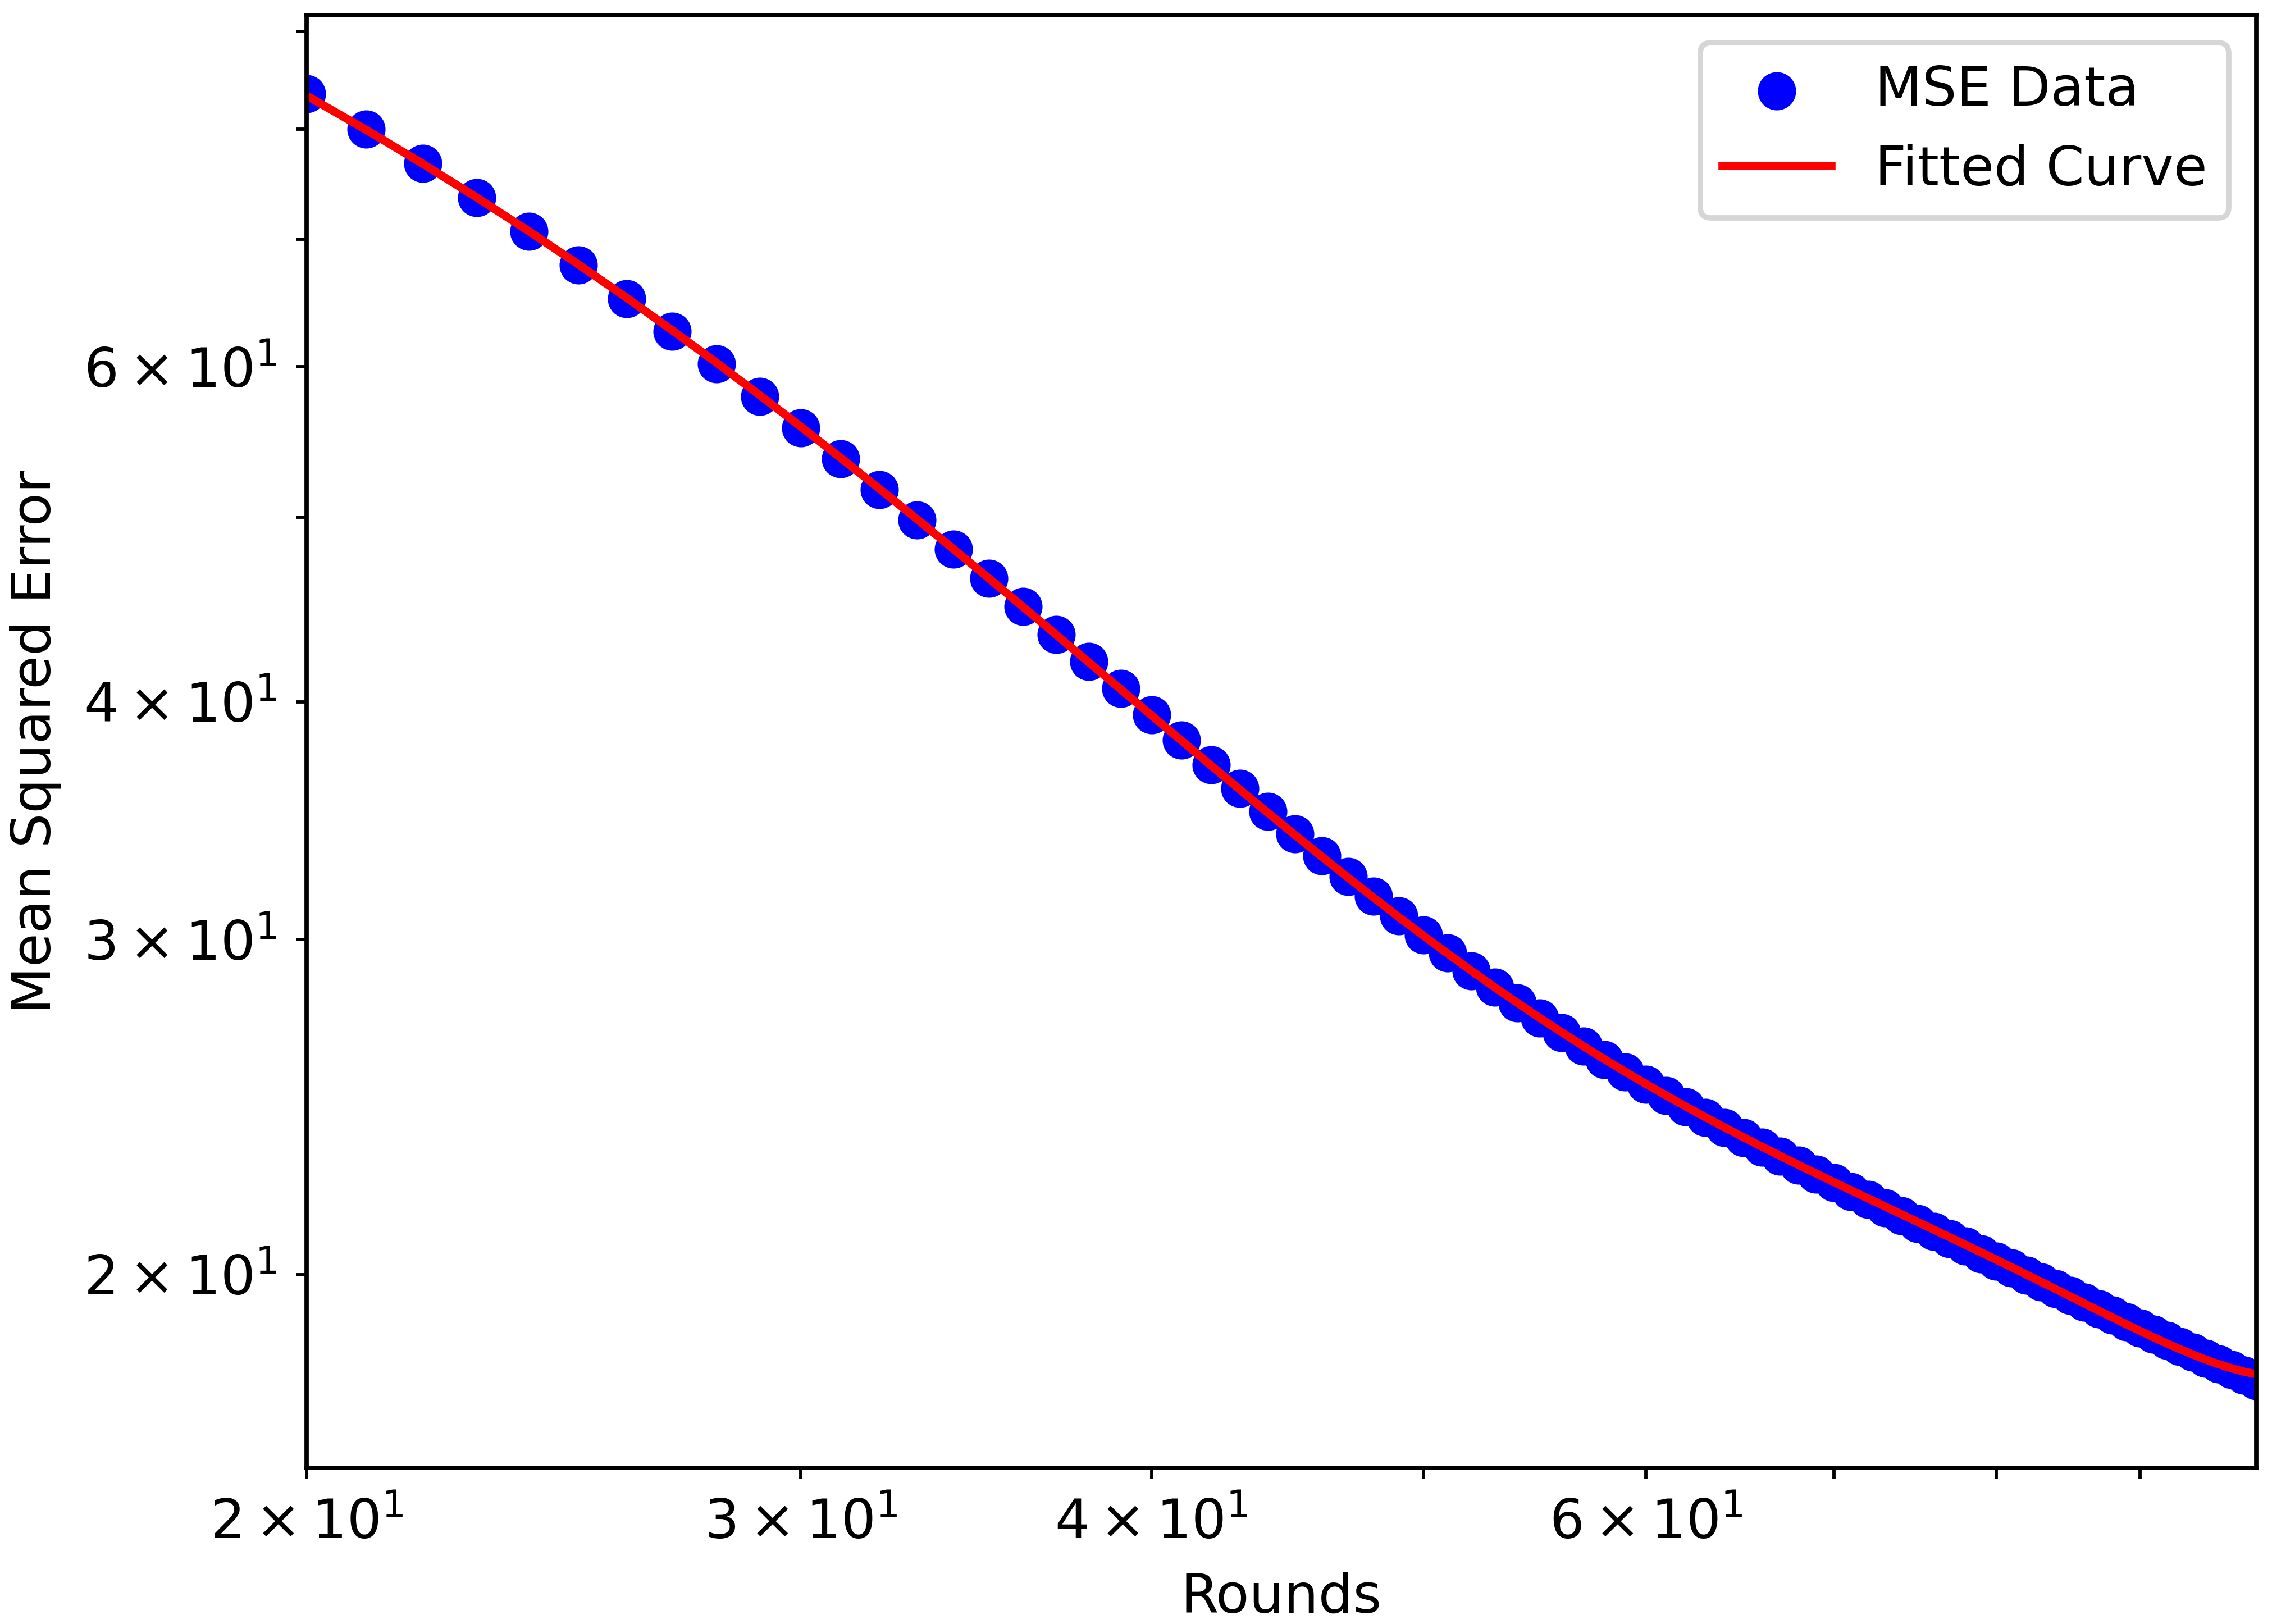
\includegraphics{figures/Simulation_outcomes/LollipopGraph/128_896/DAB/DAB_modelfitting_rounds_99_model_2.png}}
    \caption{(128, 896)-Lollipop graph - polynomial regression fit: DAB}
    \label{fig:dab_128x896lollipopgraphModelFit}
\end{figure}

\begin{figure}[]
    \centering
    \scalebox{0.8}{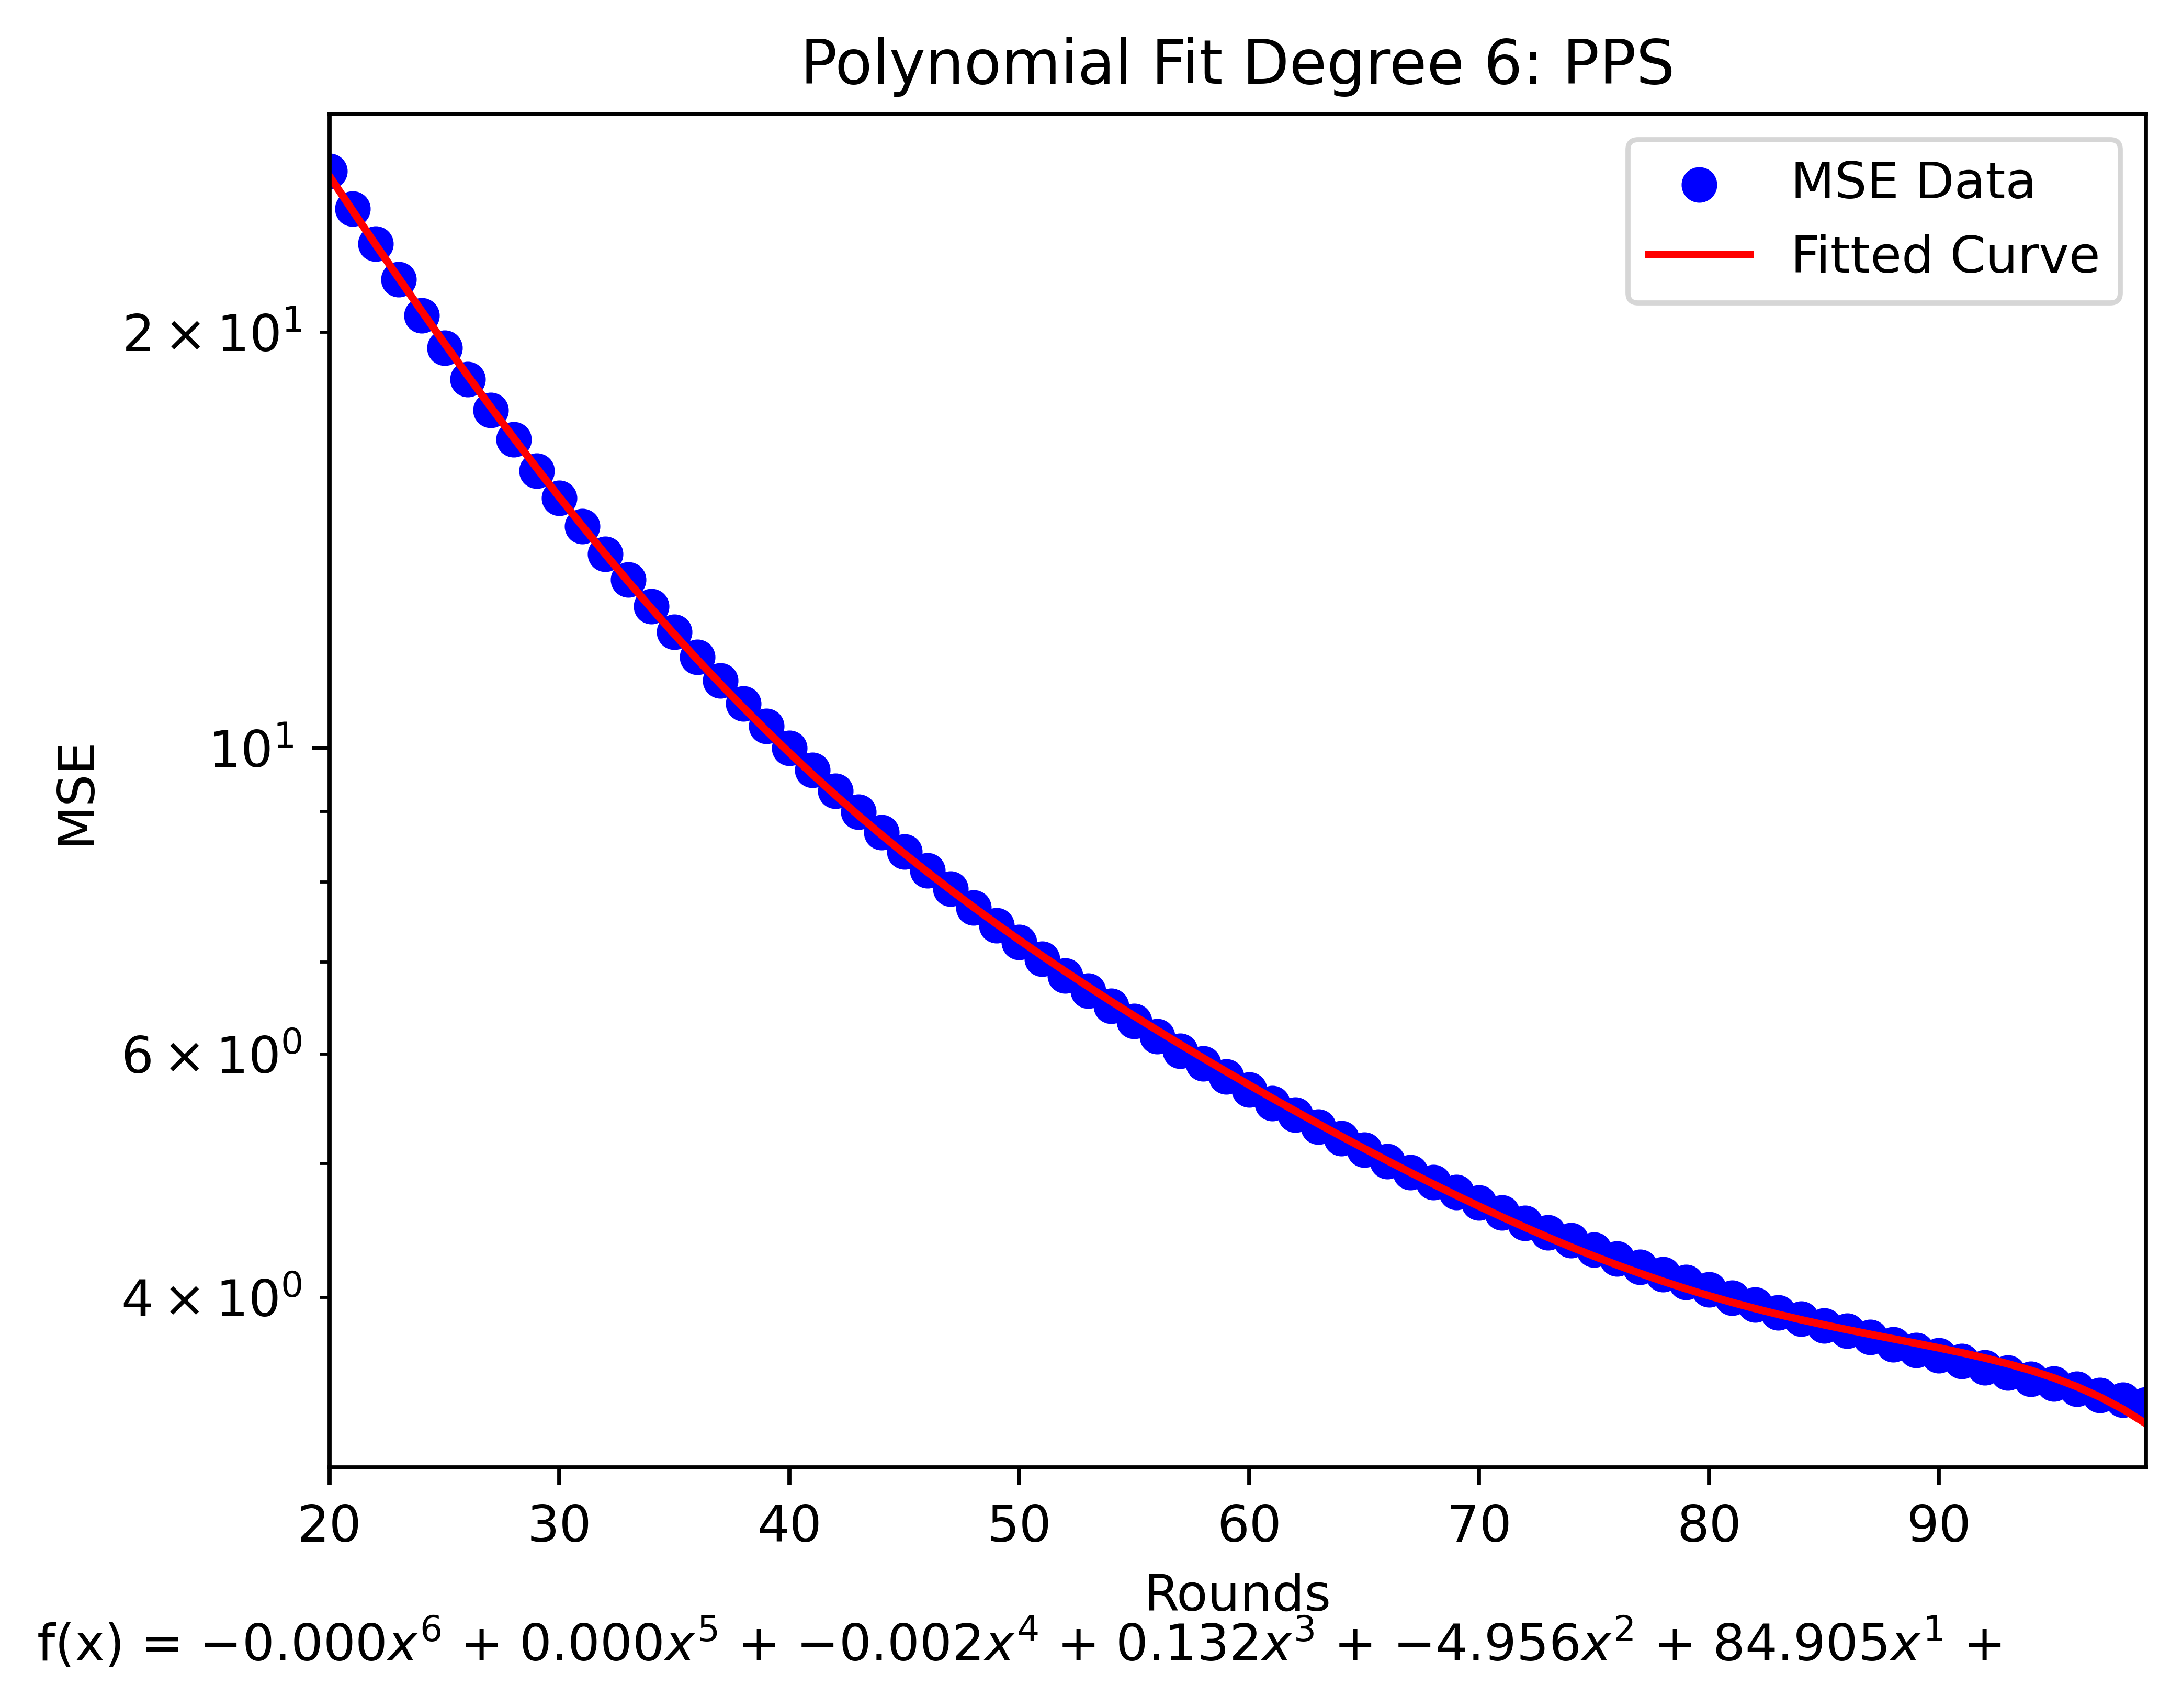
\includegraphics{figures/Simulation_outcomes/LollipopGraph/128_896/PPS/PPS_modelfitting_rounds_99_model_2.png}}
    \caption{(128, 896)-Lollipop graph - polynomial regression fit: PPS}
    \label{fig:pps_128x896lollipopgraphModelFit}
\end{figure}

\begin{figure}[]
    \centering
    \scalebox{0.8}{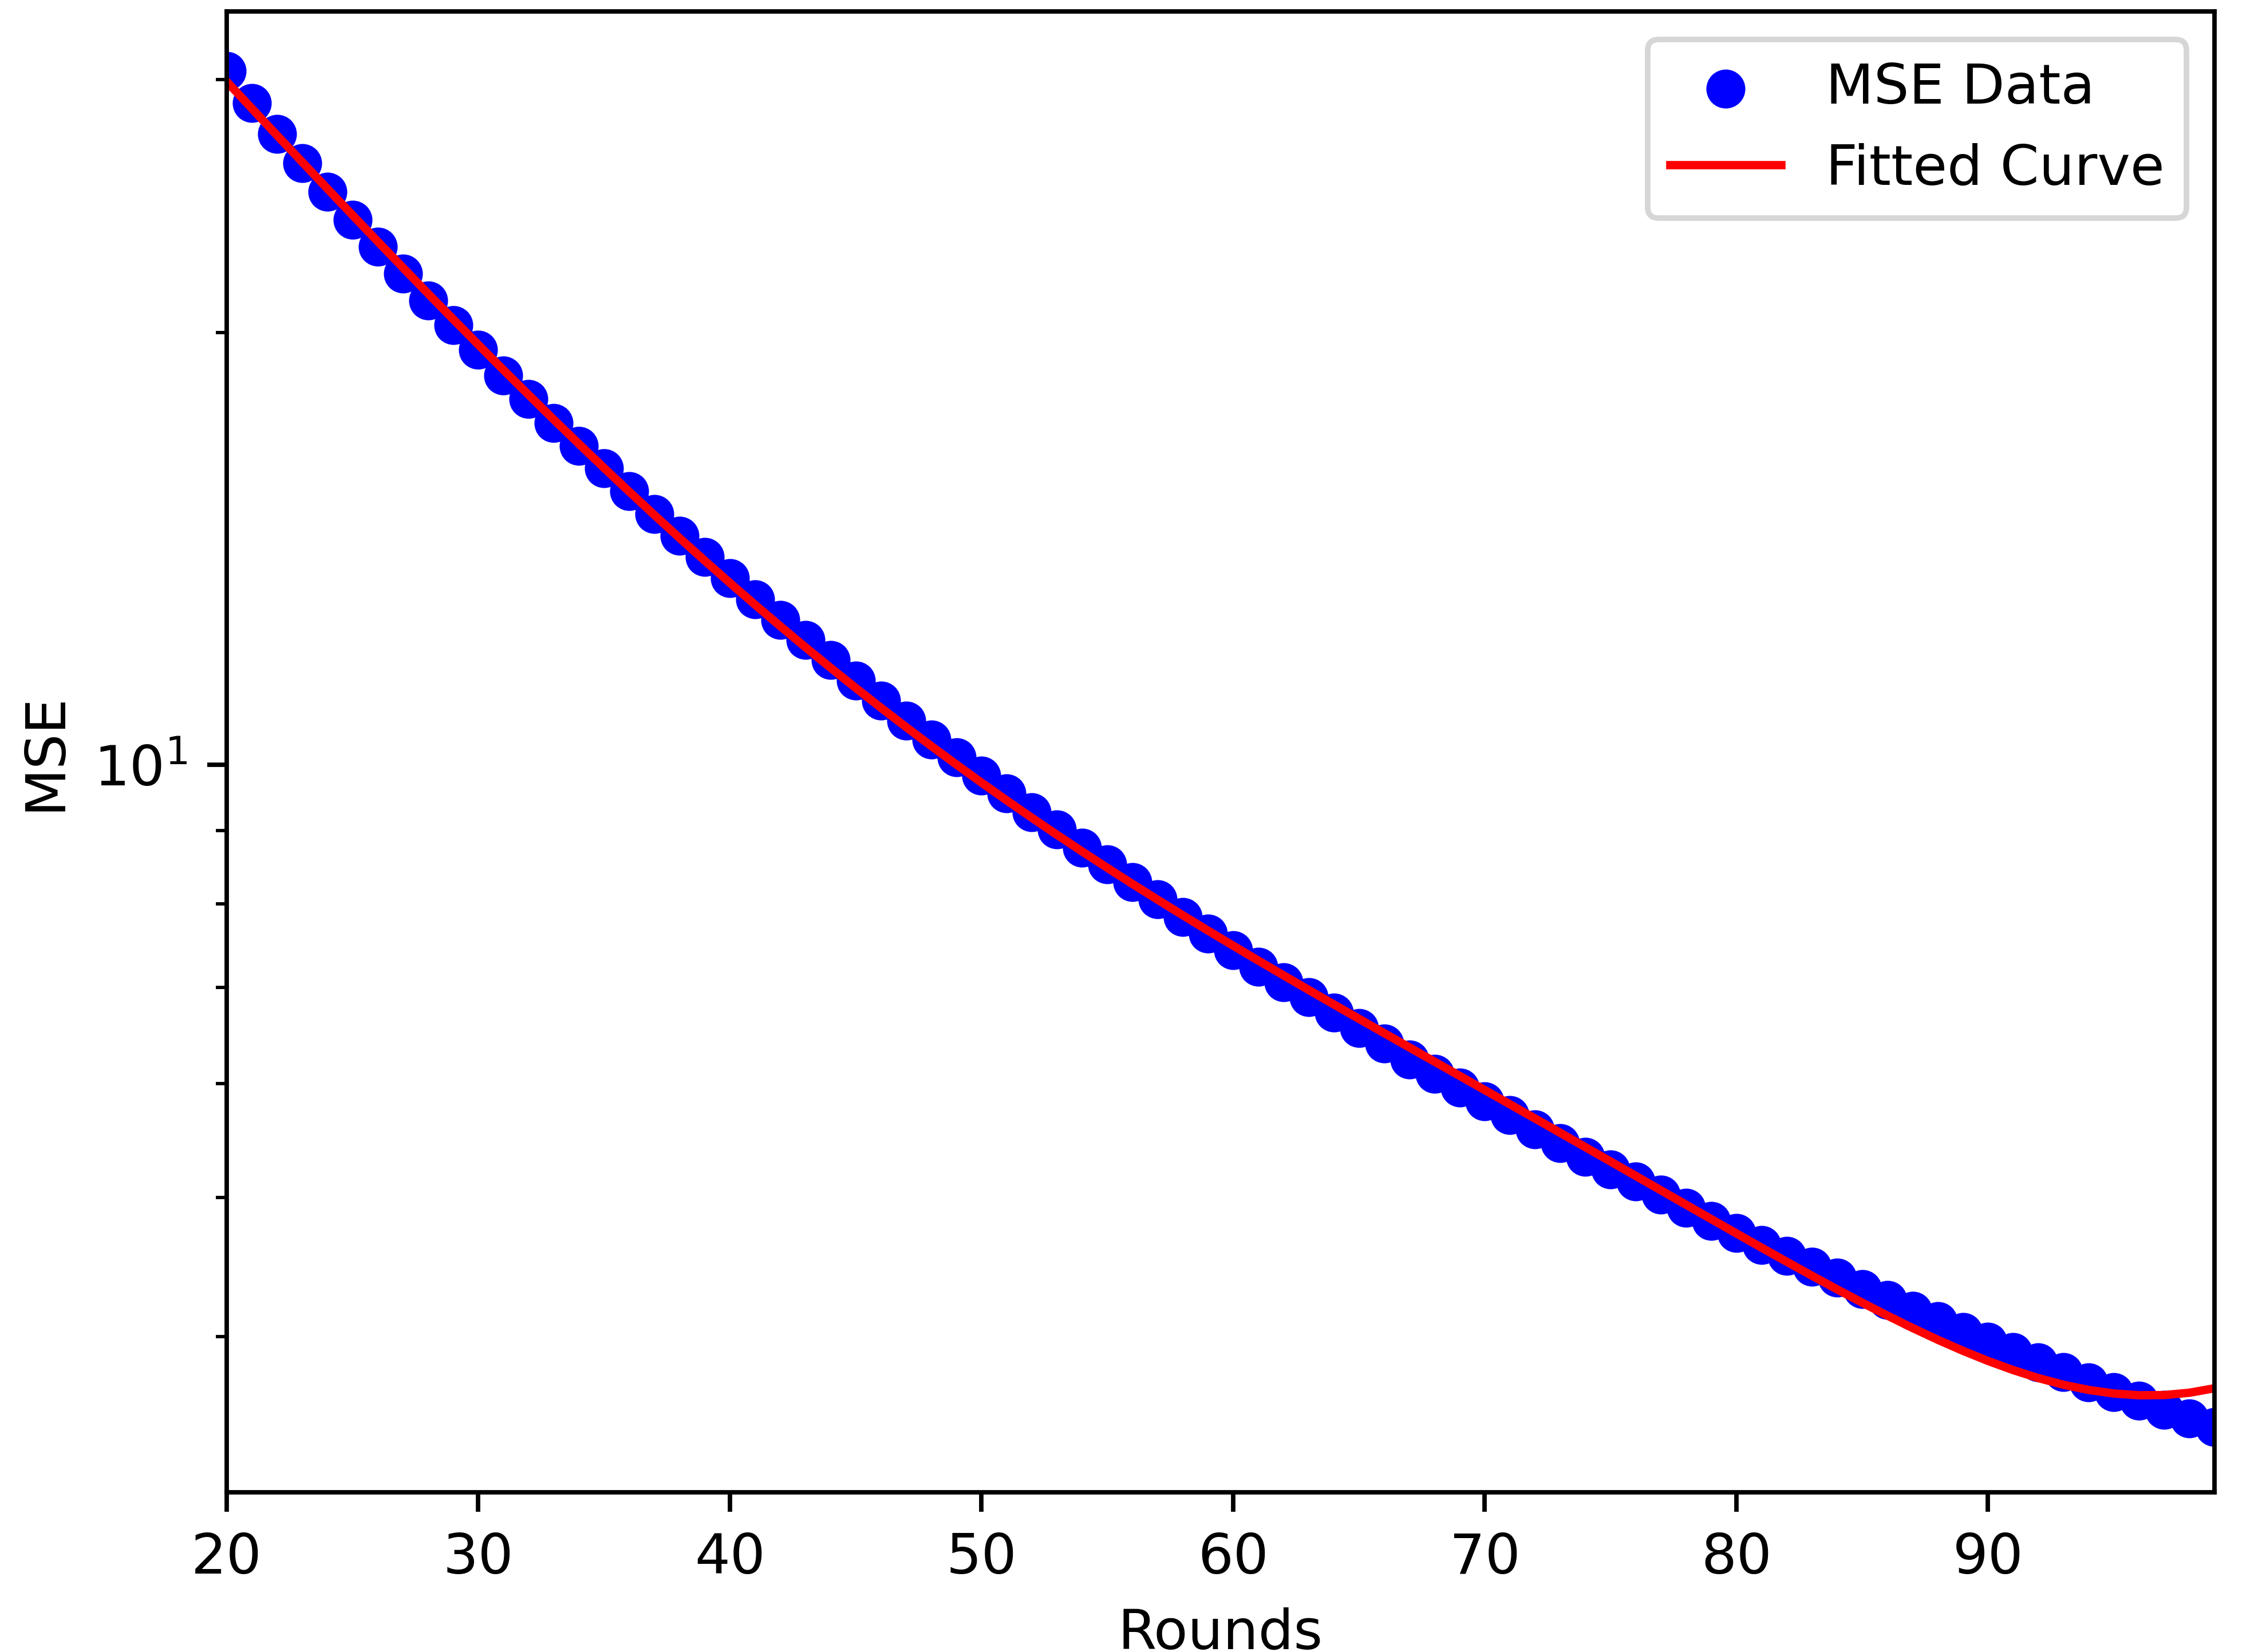
\includegraphics{figures/Simulation_outcomes/LollipopGraph/128_896/ATPPS/ATPPS_modelfitting_rounds_99_model_2.png}}
    \caption{(128, 896)-Lollipop graph - polynomial regression fit: ATPPS}
    \label{fig:atpps_128x896lollipopgraphModelFit}
\end{figure}

\begin{figure}
    \centering
    \scalebox{0.8}{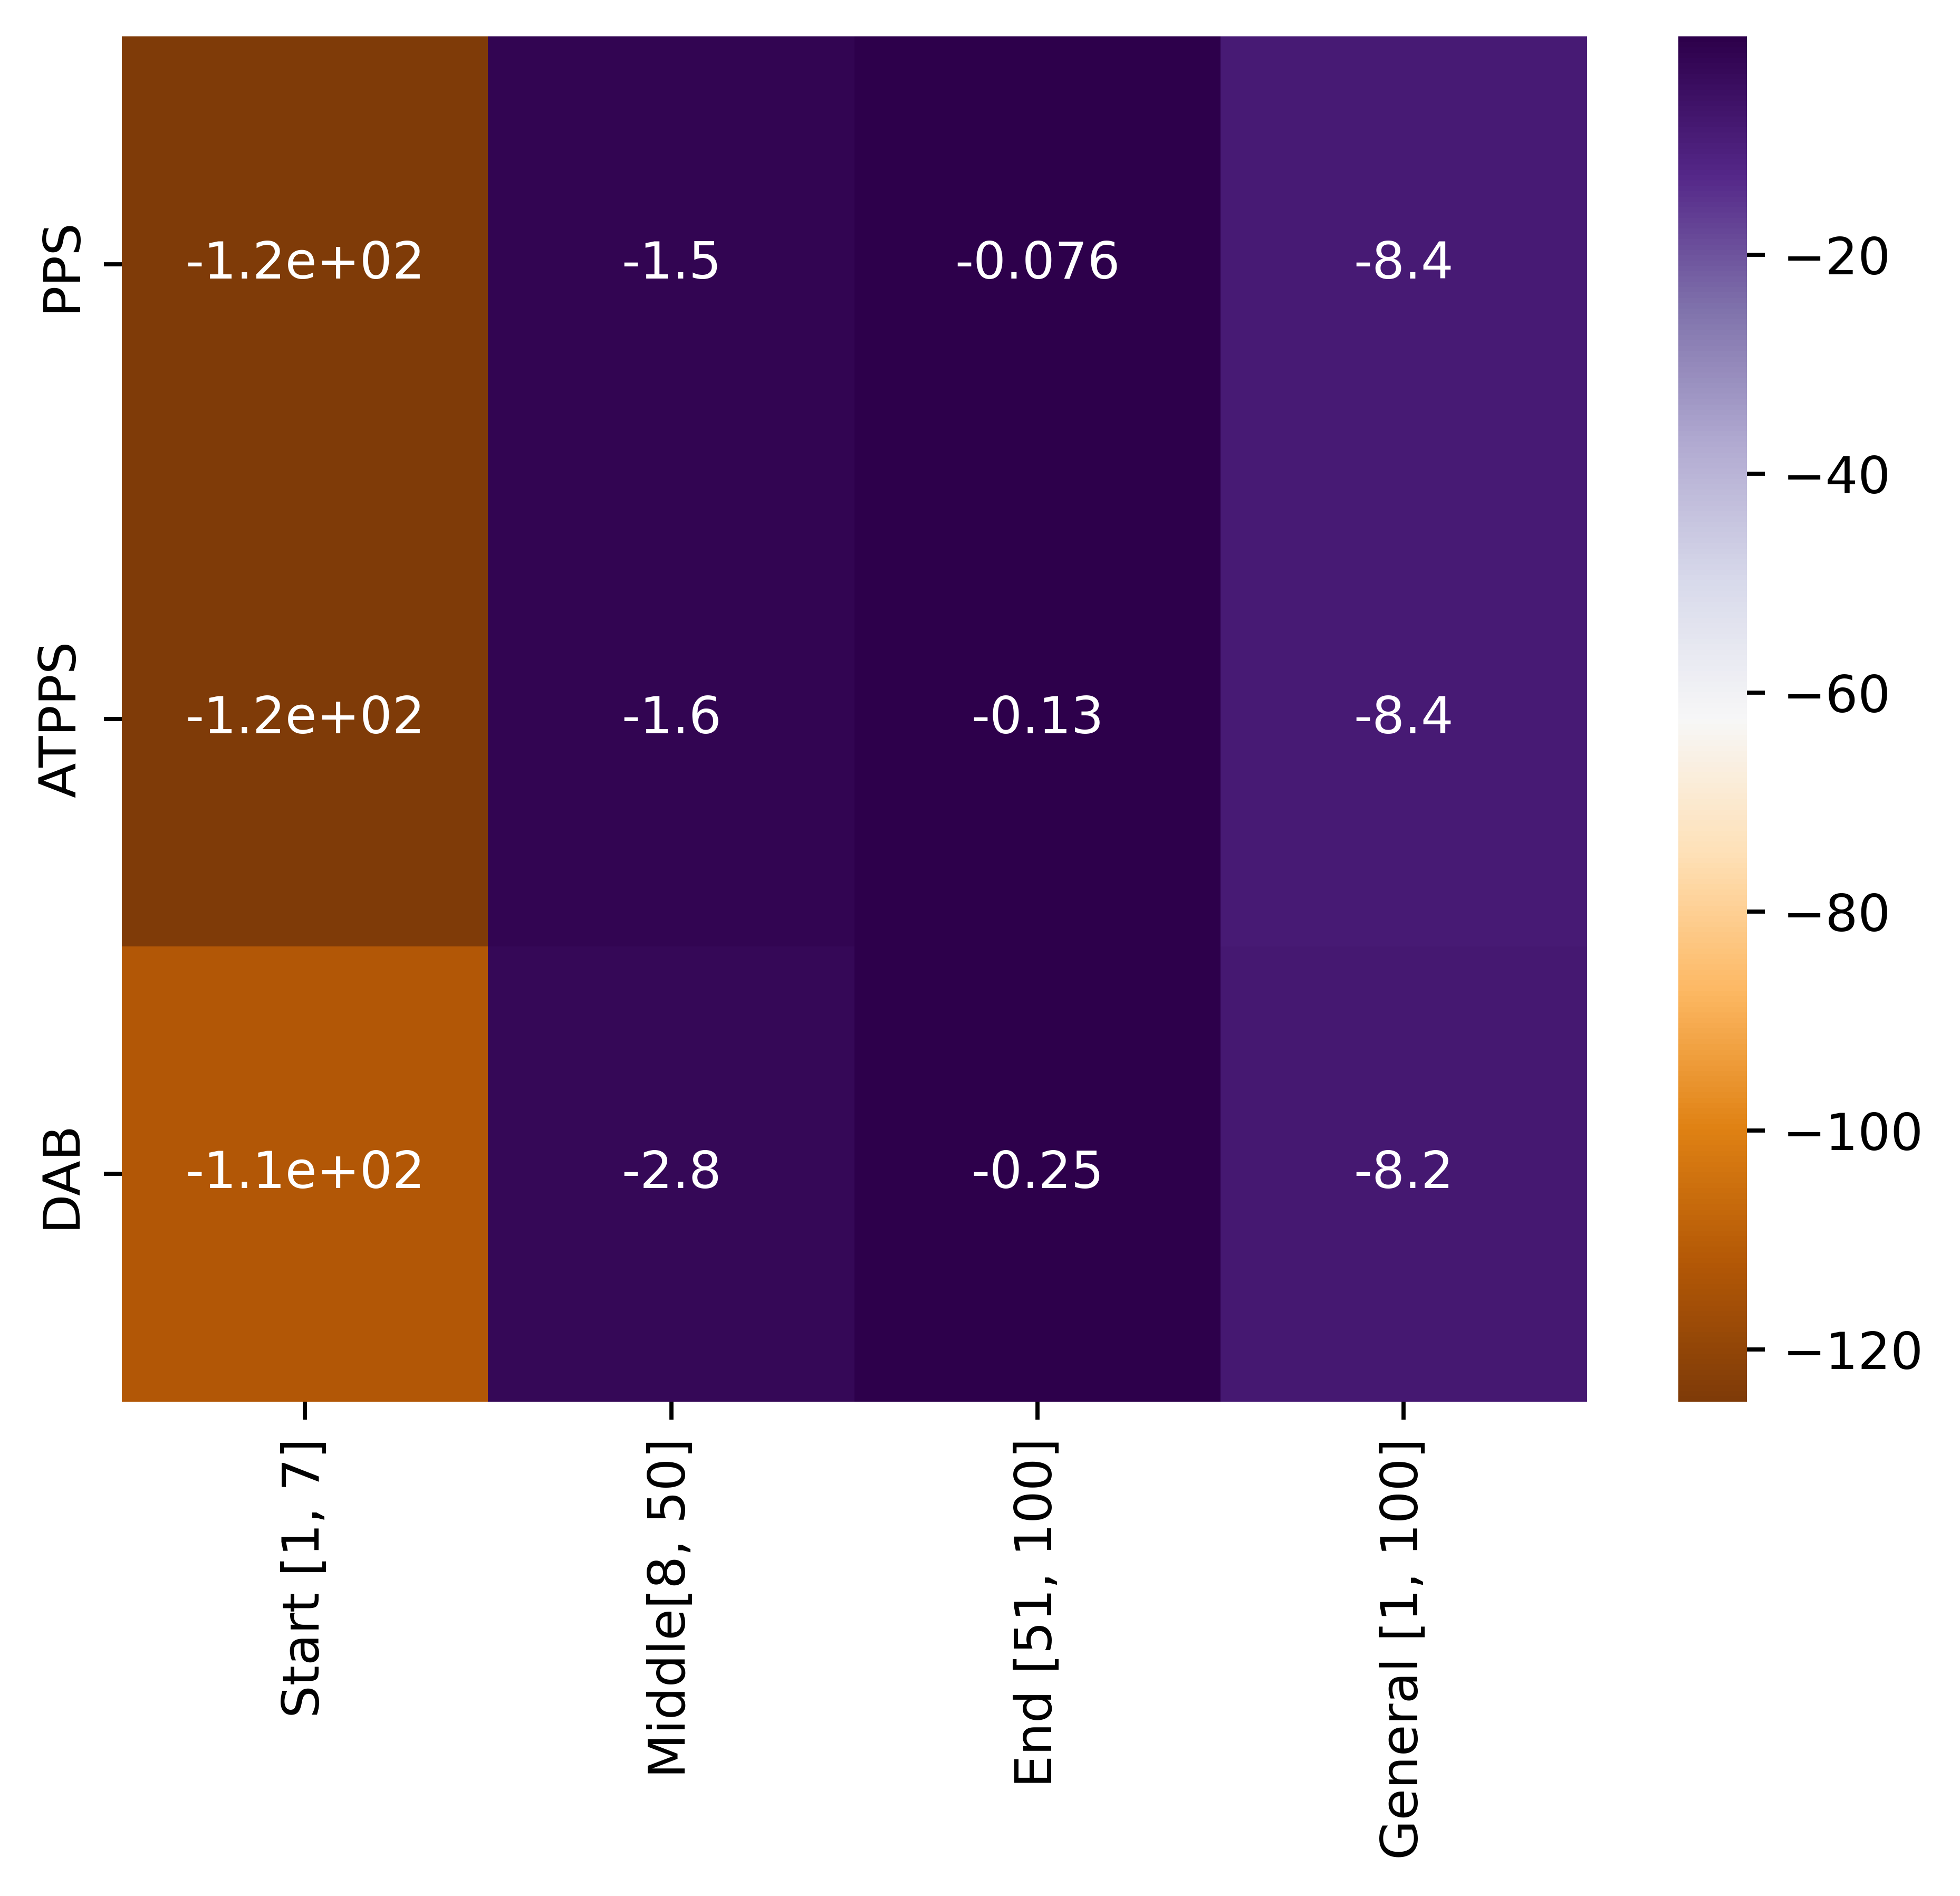
\includegraphics{figures/Simulation_outcomes/LollipopGraph/128_896/DAB_vs_PPS_vs_ATPPS_slopesheatmap_100rounds.png}}
    \caption{(128, 896)-Lollipop graph: heat map of slopes per region}
    \label{fig:128_896lollipopslopes}
\end{figure}

\subsection{(896, 128) Lollipop Graph}\label{subsec:896_128lollipop}
Now that more nodes are assigned to the clique and taken from the path compared to the initial experiment where the clique and the path had the same number of nodes, the discrepancy between the Push-Pull Sum based and the DAB algorithms is more obvious, as shown in figure \ref{fig:896_128lollipopgraphMSEperRoundLogLog}. This is also indicated by the slopes. In the start region the Push-Pull Sum based algorithms both balance the network with the (896, 128)-Lollipop graph more quickly, achieving slopes of -140 in this initial region, compared to -130 (figure \ref{fig:896x128lollipopslopes}) in the (512, 512)-Lollipop graph. The overall MSE is also lower for the (896, 128)-Lollipop graph, where the error is reduced to a value of 3.27 for the network where the ATPPS is applied and 3.59 for the network where PPS is applied as a load balancing strategy. The MSE values for the (512, 512)-Lollipop graph are higher, where the MSE data of the ATPPS shows values of 13.83 and for the PPS 14.71. However, no significant advantage of the ATPPS over the PPS is observed. The DAB struggles to achieve good performance in reducing error, showcased by the immense discrepancy between the MSE values after 100 rounds. For the (512, 512)-Lollipop graph experiments the DAB achieved values of 108.90, in the experiment of (896, 128)-Lollipop graph the value that the network ends up with is at 542.09, which is nearly five times as much.

The best-fit polynomials fitted to the MSE data of the load balancing algorithms are of degree 3 for the DAB MSE data and of degree 4 for the PPS-based algorithms MSE data. The polynomial for the DAB MSE data follows the equation: $MSE_r=-1.936\times 10^{-4}r^{3}+0.05r^{2}-5.33r+745.95$ (figure \ref{fig:dab_896x128lollipopgraphModelFit}). The polynomial for the Push-Pull Sum based algorithms follow the equation: $MSE_r=2.00\times 10^{-7}r^{4}-6.01\times 10^{-5}r^{3}+6.95\times 10^{-3}r^{2}-0.39r+13.44$ (figure \ref{fig:pps_896x128lollipopgraphModelFit}) for the PPS and $MSE_r=2.28\times 10^{-7}r^{4}-6.77\times 10^{-5}r^{3}+7.68\times 10^{-3}r^{2}-0.42r+13.62$ for the ATPPS (figure \ref{fig:atpps_896x128lollipopgraphModelFit}). 
\begin{figure}[]
    \centering
    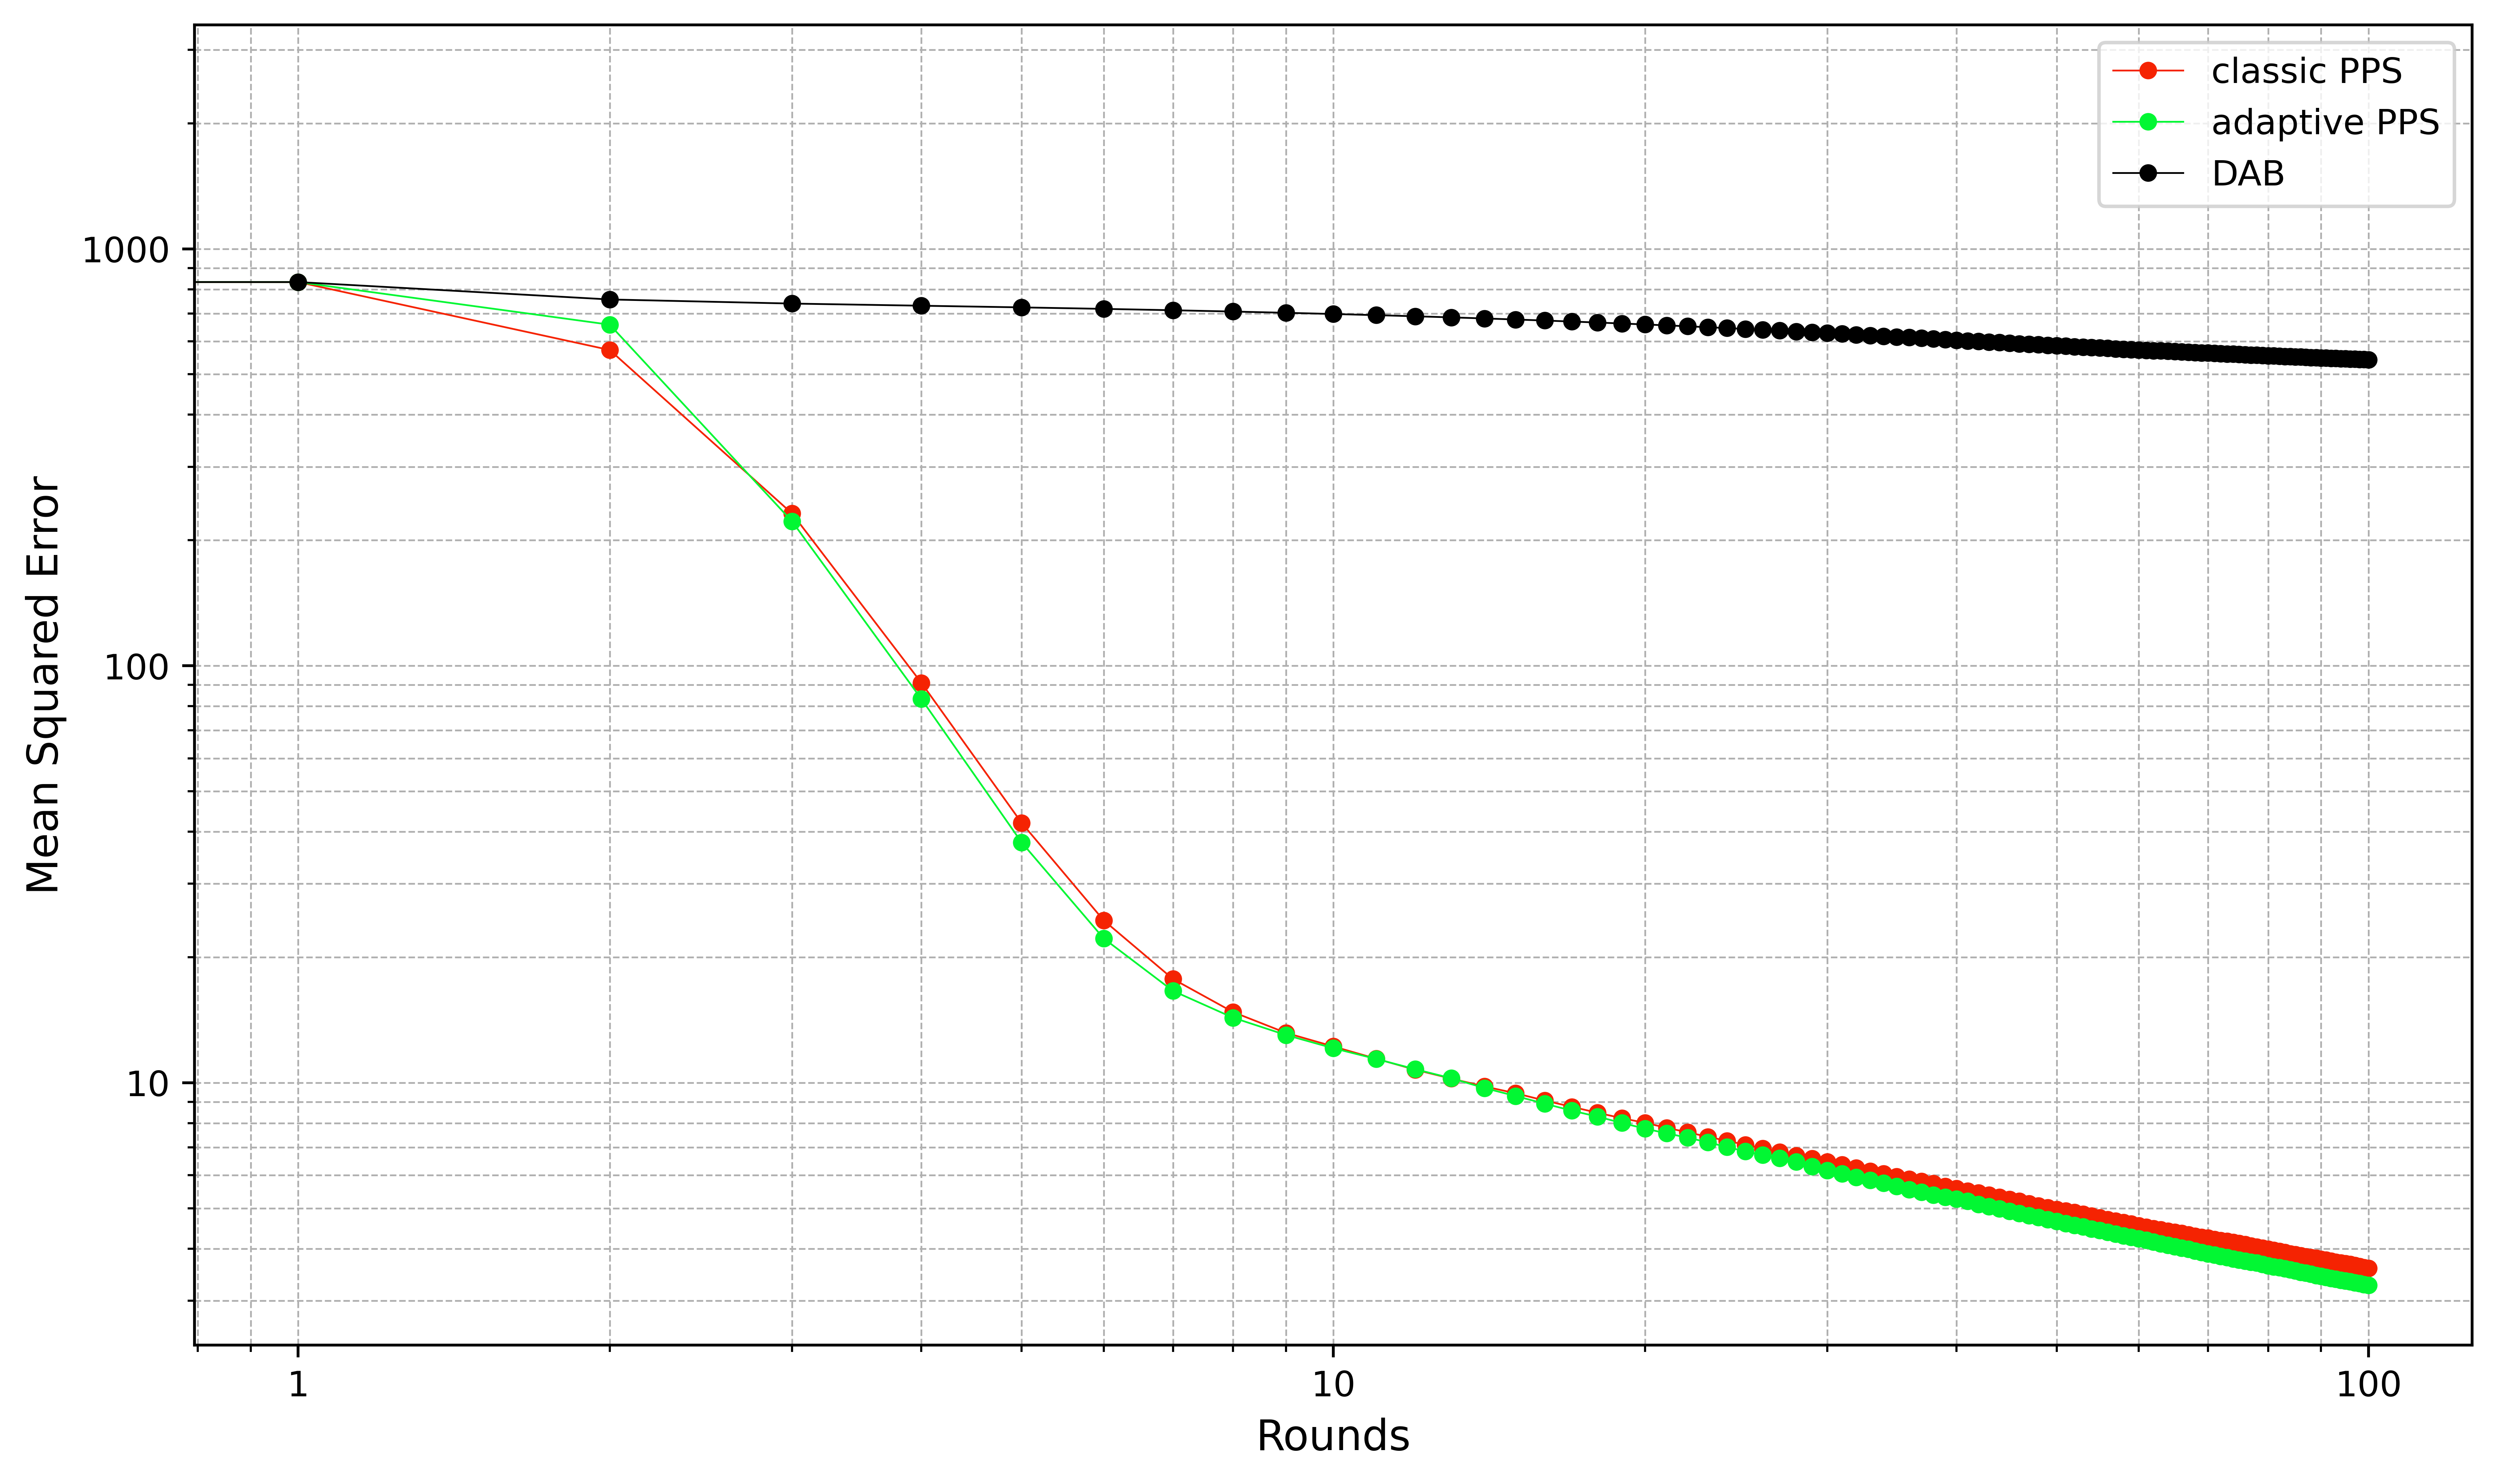
\includegraphics[width=\linewidth]{figures/Simulation_outcomes/LollipopGraph/896_128/DAB_vs_PPS_LG_r100_n1024_averaged_loglog.png}
    \caption{(896, 128)-Lollipop graph: mean squared error per rounds (log-log)}
    \label{fig:896_128lollipopgraphMSEperRoundLogLog}
\end{figure}

\begin{figure}[]
    \centering
    \scalebox{0.8}{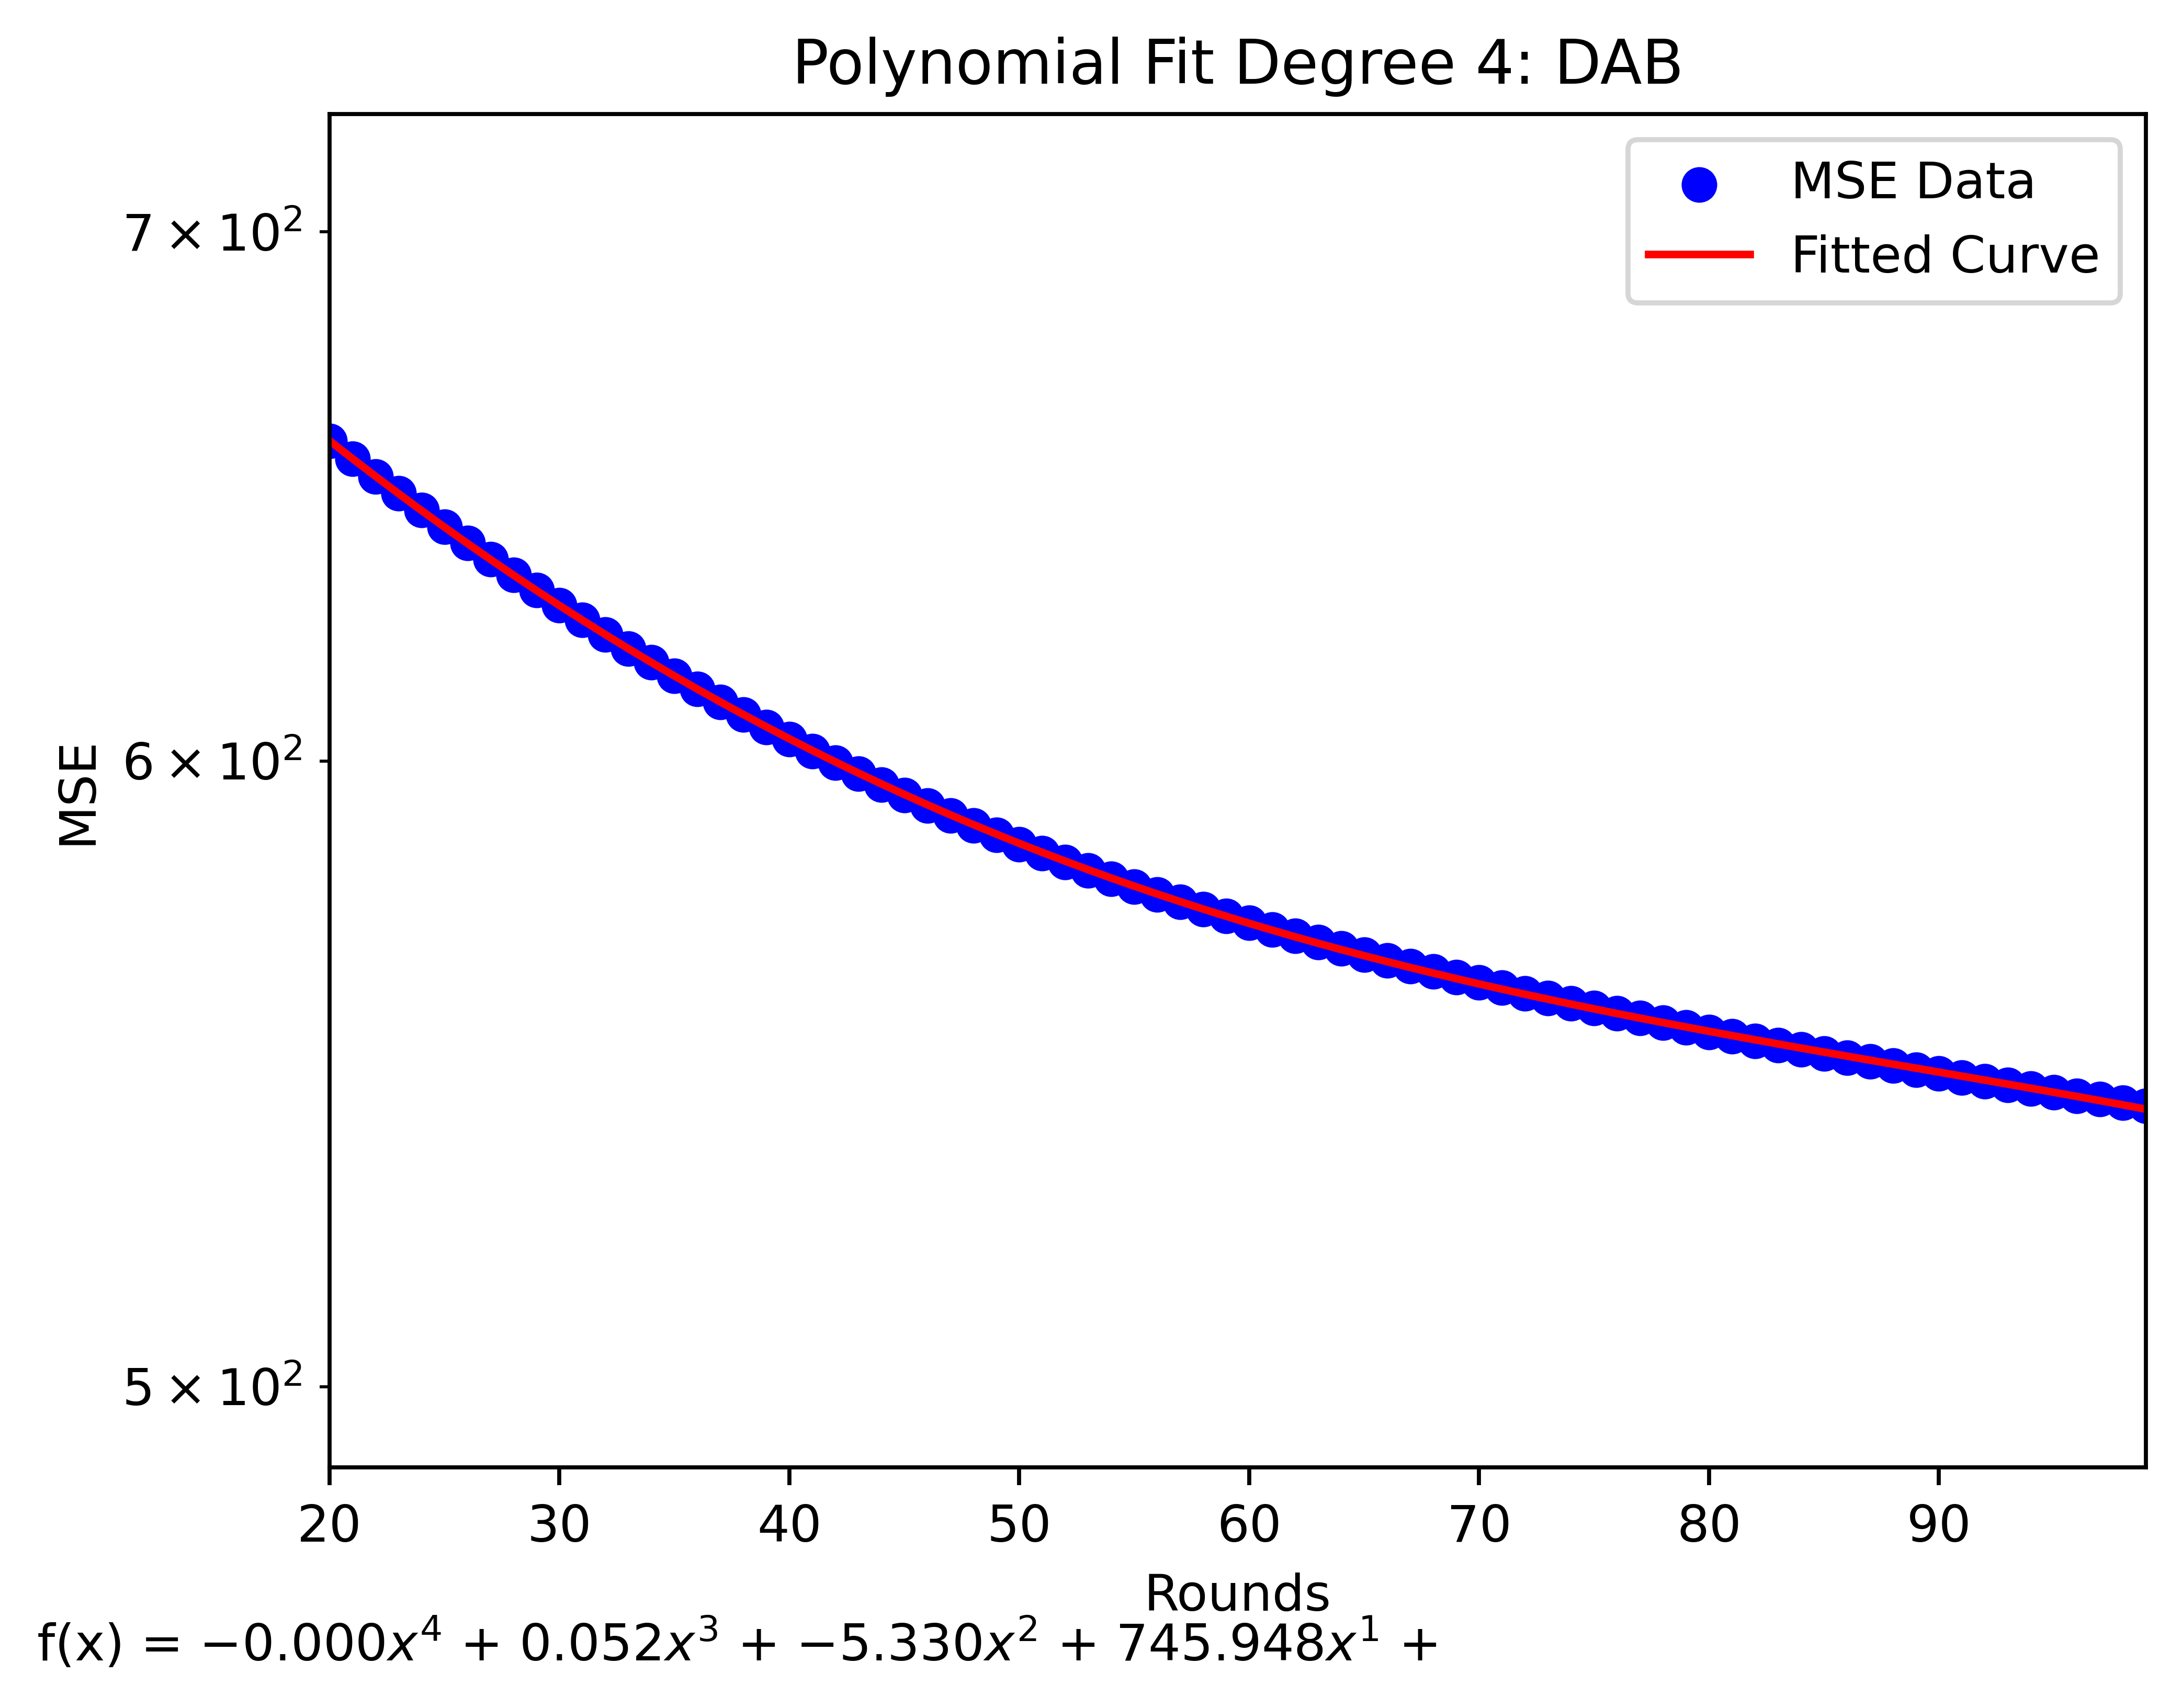
\includegraphics[width=\linewidth]{figures/Simulation_outcomes/LollipopGraph/896_128/DAB/DAB_modelfitting_rounds_99_model_2.png}}
    \caption{(896, 128)-Lollipop graph - polynomial regression fit: DAB}
    \label{fig:dab_896x128lollipopgraphModelFit}
\end{figure}

\begin{figure}[]
    \centering
    \scalebox{0.8}{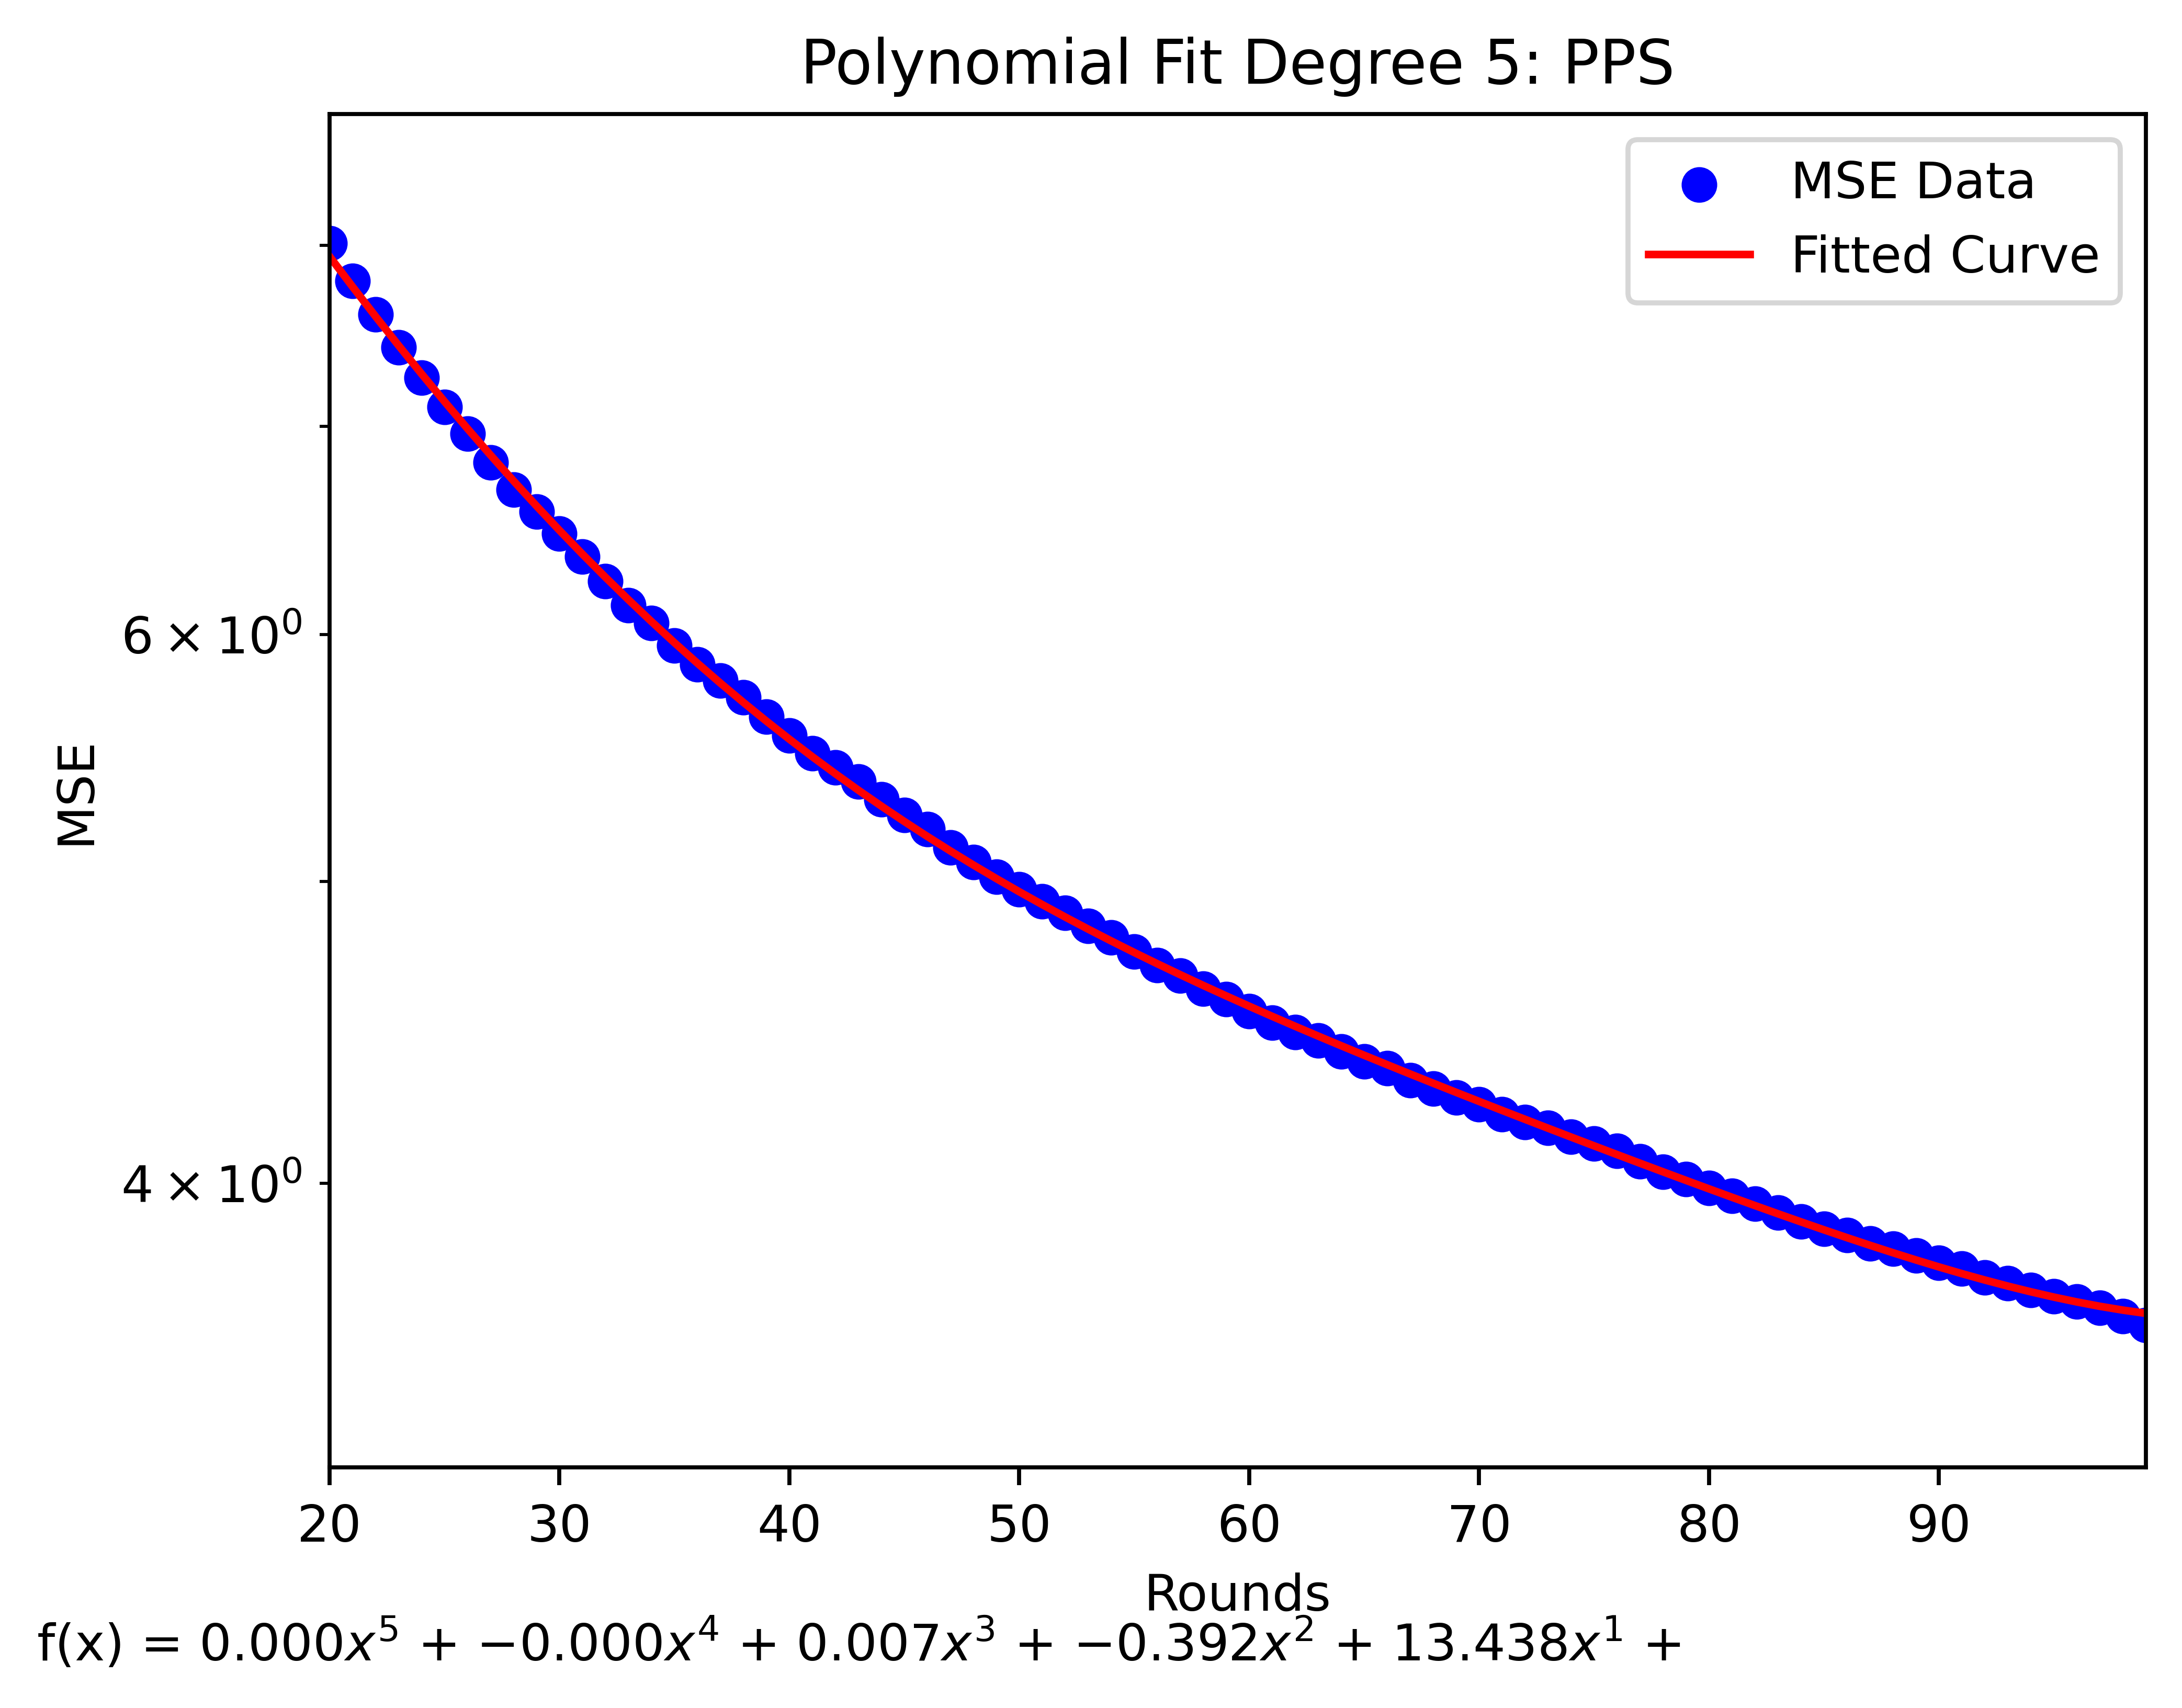
\includegraphics{figures/Simulation_outcomes/LollipopGraph/896_128/PPS/PPS_modelfitting_rounds_99_model_2.png}}
    \caption{(896, 128)-Lollipop graph - polynomial regression fit: PPS}
    \label{fig:pps_896x128lollipopgraphModelFit}
\end{figure}

\begin{figure}[]
    \centering
    \scalebox{0.8}{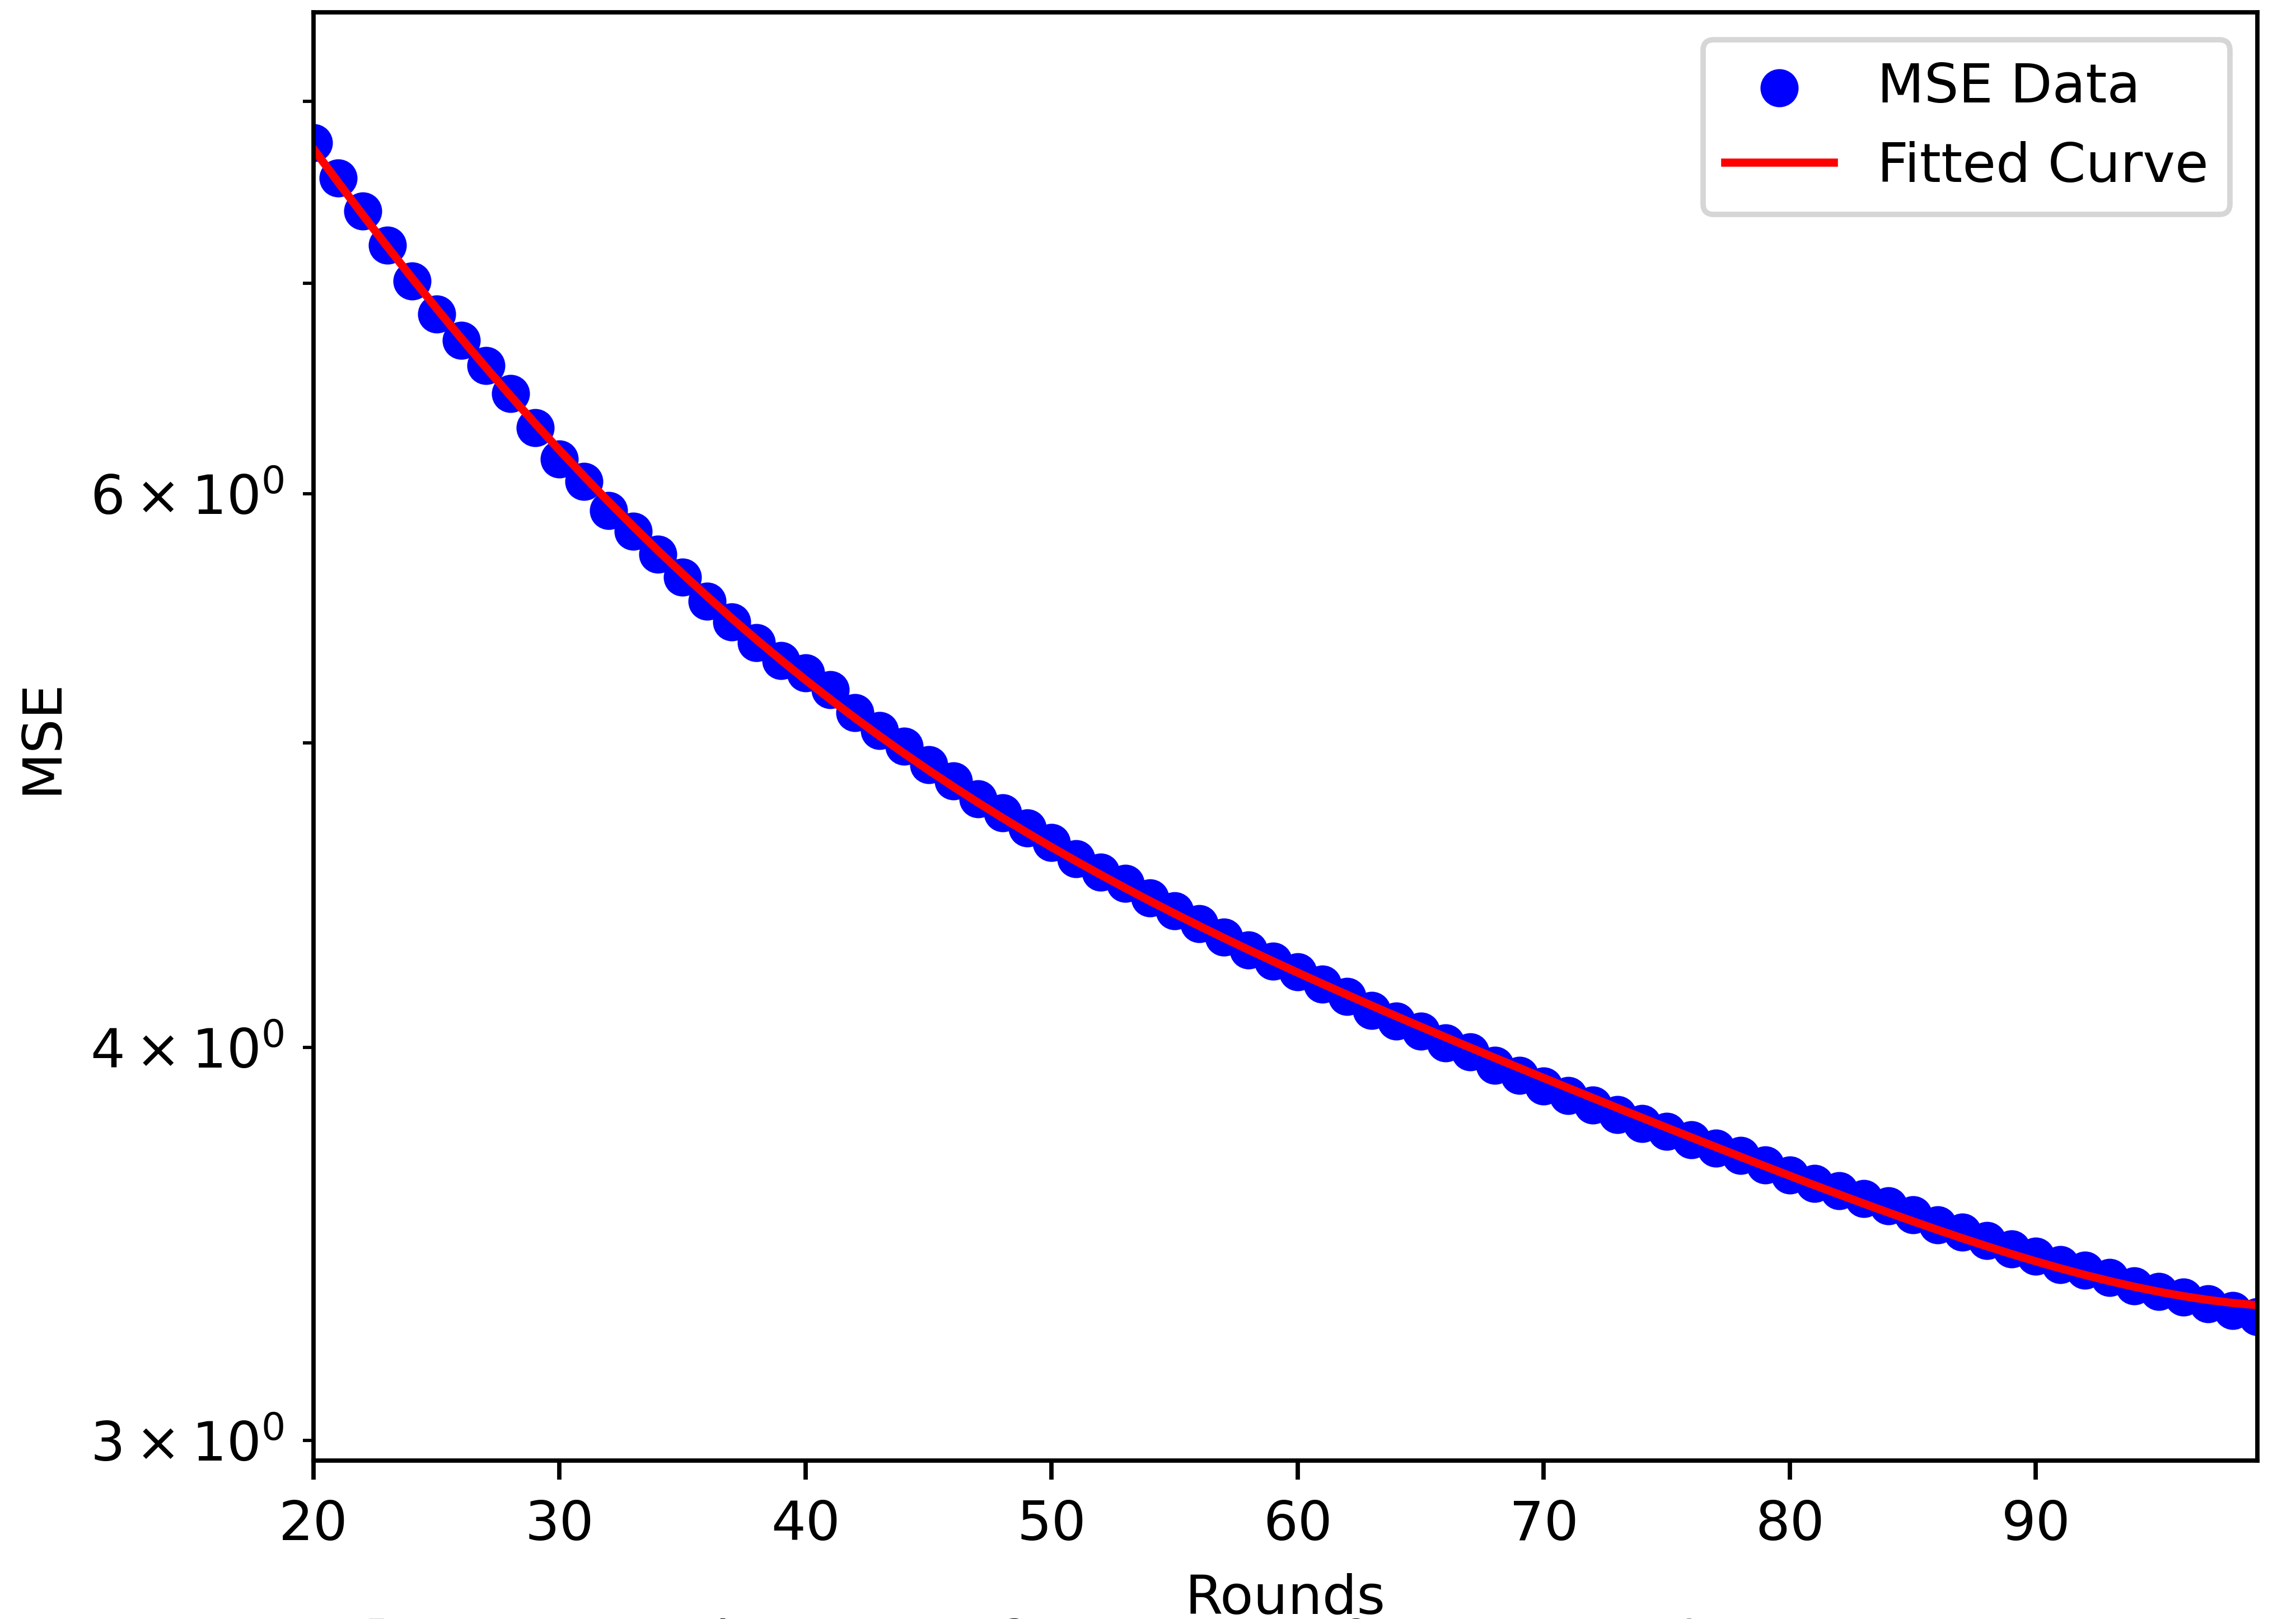
\includegraphics[width=\linewidth]{figures/Simulation_outcomes/LollipopGraph/896_128/ATPPS/ATPPS_modelfitting_rounds_99_model_2.png}}
    \caption{(896, 128)-Lollipop graph - polynomial regression fit: ATPPS}
    \label{fig:atpps_896x128lollipopgraphModelFit}
\end{figure}

\begin{figure}
    \centering
    \scalebox{0.8}{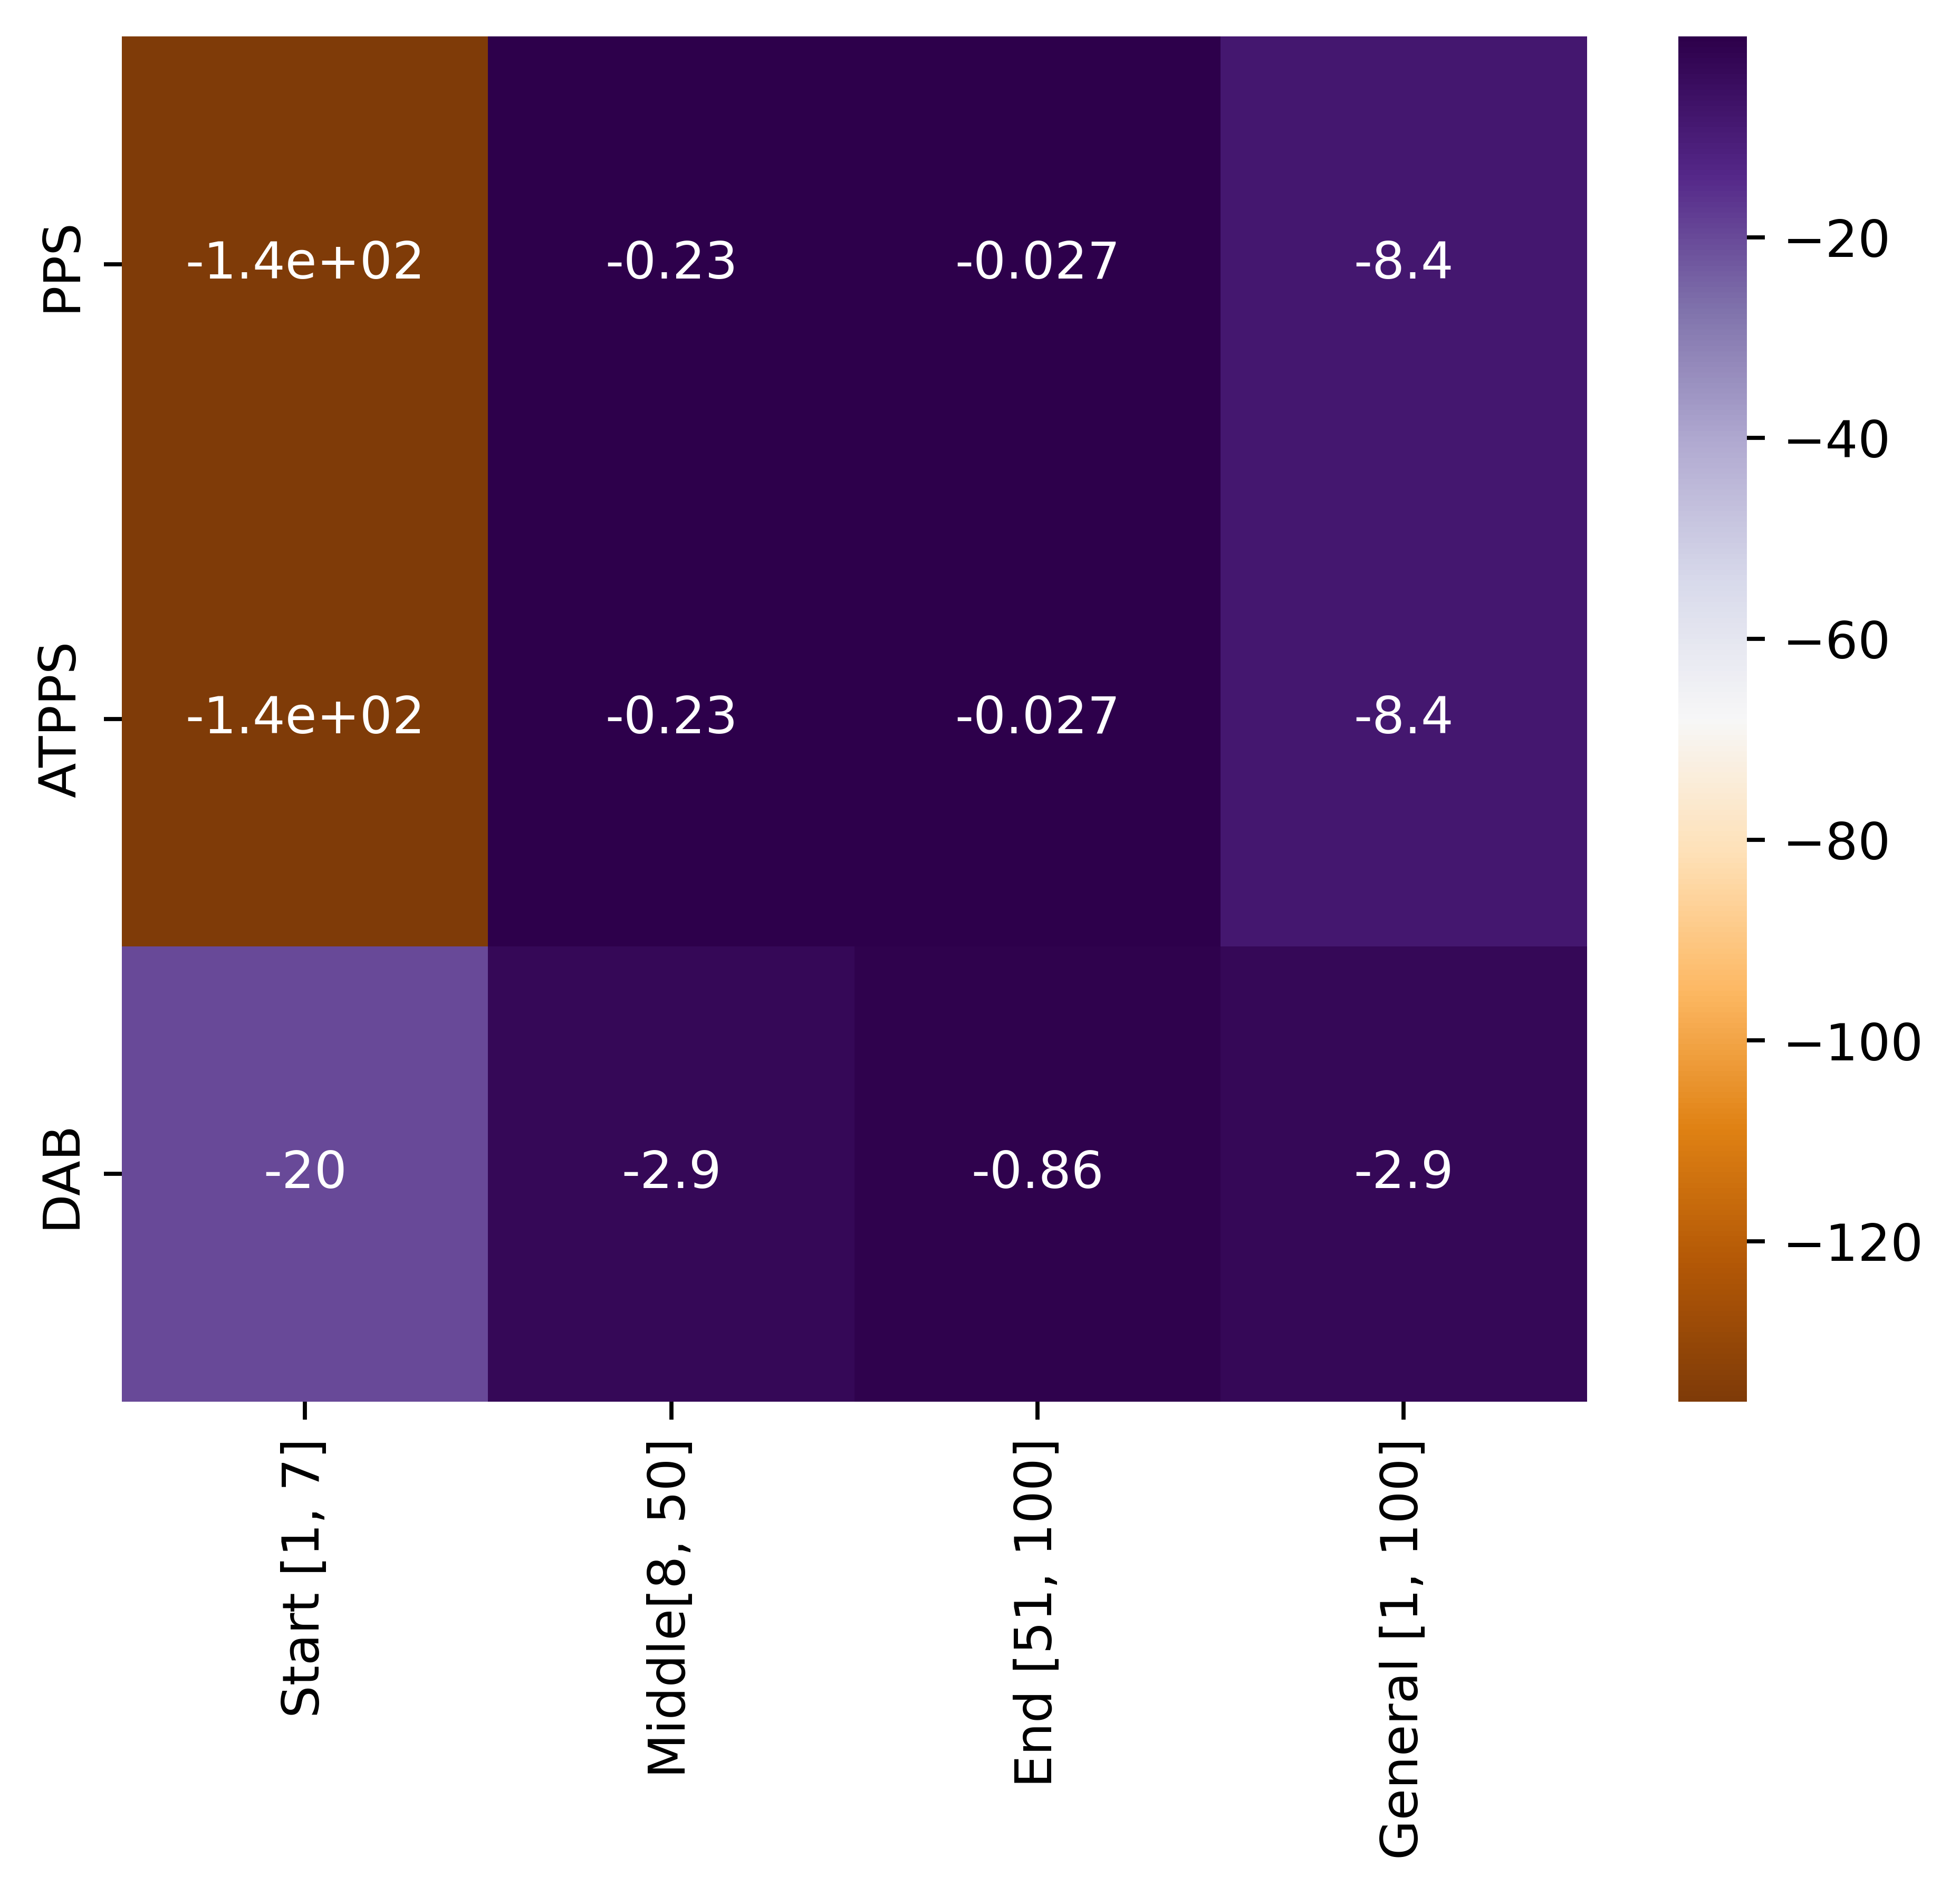
\includegraphics{figures/Simulation_outcomes/LollipopGraph/896_128/DAB_vs_PPS_vs_ATPPS_slopesheatmap_100rounds.png}}
    \caption{(896, 128) Lollipop Graph: heat map of slopes per region}
    \label{fig:896x128lollipopslopes}
\end{figure}

\section{Ring of Cliques}\label{sec:ringofcliques}
\subsection{32x32 Ring of Cliques}\label{subsec:32_32ROC}
In the early rounds, PPS and ATPPS exhibit the fastest MSE reduction showcased by a very steep downwards trend between rounds 1 and 5 in figure \ref{fig:atppsRingOfCliquesLog_LogLog} b). Both Push-Pull Sum based approaches start with faster convergence rates compared to DAB. The initial steep downwards slope of -200 for each Push-Pull Sum based algorithm as depicted in figure \ref{fig:ringOfCliquesslopes} within the first 5 rounds is due to the unbalanced state of each clique. The Push-Pull Sum based approaches have shown to be outperforming the DAB algorithm for Complete graphs. While the cliques are still unbalanced the Push-Pull Sum based algorithms achieve faster convergence. After the cliques are balanced round by round the DAB algorithm catches up especially between the rounds 6 to 40 where the slopes are -48 compared to $\sim-2$ for the Push-Pull Sum based algorithms. Nodes within cliques tend to converge quickly internally due to their dense interconnections for the Push-Pull Sum based algorithms. However, load balancing between cliques, especially when the nodes select for random neighbors is slower, creating bottlenecks for global convergence (this is especially the case for the PPS, whichs curve starts to stagnate between round 10 to 100). Due to the determistic nature of the DAB, the bridging nodes choose nodes outside of their cliques, once the load is balanced within the clique, and spread the load to other cliques. The ATPPS algorithm achieves better results compared to the PPS, since it has a similar mechanism in this scenario like the DAB, prioritizing communication between cliques (where differences in loads are more significant) over redundant communication within cliques (where loads are already close to balanced). This is mirrored in the behavior of the curve after round 10. Again, the ATPPS acts as a compromise solution between the PPS and the DAB achieving results close to them of the DAB algorithm. Overall, at round 100 the DAB achieved a MSE of $\sim 6.55$, the PPS a MSE of 19.80 and the ATPPS a MSE of 8.42.

The polynomial fit for the DAB algorithm is: $MSE_r=1.04\times 10^{-6}r^{4}-2.941\times 10^{-4}r^{3}+0.03r^{2}-1.66r+45.30$ (figure \ref{fig:dabRingOfCliquesModelFit}). Thus the MSE as a function of rounds is modeled by a fourth degree polynomial. The PPS MSE data of rounds 20 to 100 is fitted to a linear regression model following the equation: $MSE_r=-0.05r+24.70$ (figure \ref{fig:ppsRingOfCliquesModelFit}). The negative slope indicates a consistent reduction in MSE with each round in this region, but the value -0.05 is relatively small. This suggests that the PPS algorithm achieves slow and steady progress toward load balancing. The linear fit highlights that PPS achieves only gradual improvement in balancing the load in the Ring of Cliques topology. The reason for that is that PPS focuses on a push-pull mechanism that is, relying on random neighbor interactions. In the Ring of Cliques, inter-clique connections are sparse, and PPS lacks a mechanism to prioritize balancing between these sparsely connected regions. As a result, its performance is bottlenecked by the topology. The linearity of the model suggests a uniform rate of error reduction across rounds, without any acceleration observed in other methods (like DAB). The logarithmic model for the ATPPS algorithm is given as:
$\log{(MSE_r)}=-7.59\log{(r)}+43.26$ (figure \ref{fig:atppsRingOfCliquesModelFit}). By exponentiating this equation, the relationship between the MSE and the number of rounds is: $MSE_r=10^{43.26}*r-7.59$. The steep negative slope of value -7.59 in the log-log fit indicates a rapid decrease in MSE as the number of rounds increases. This suggests that ATPPS achieves exponentially faster convergence compared to PPS, especially in the early rounds of load balancing.

\begin{figure}[!ht]
    \centering
        \subfloat[]{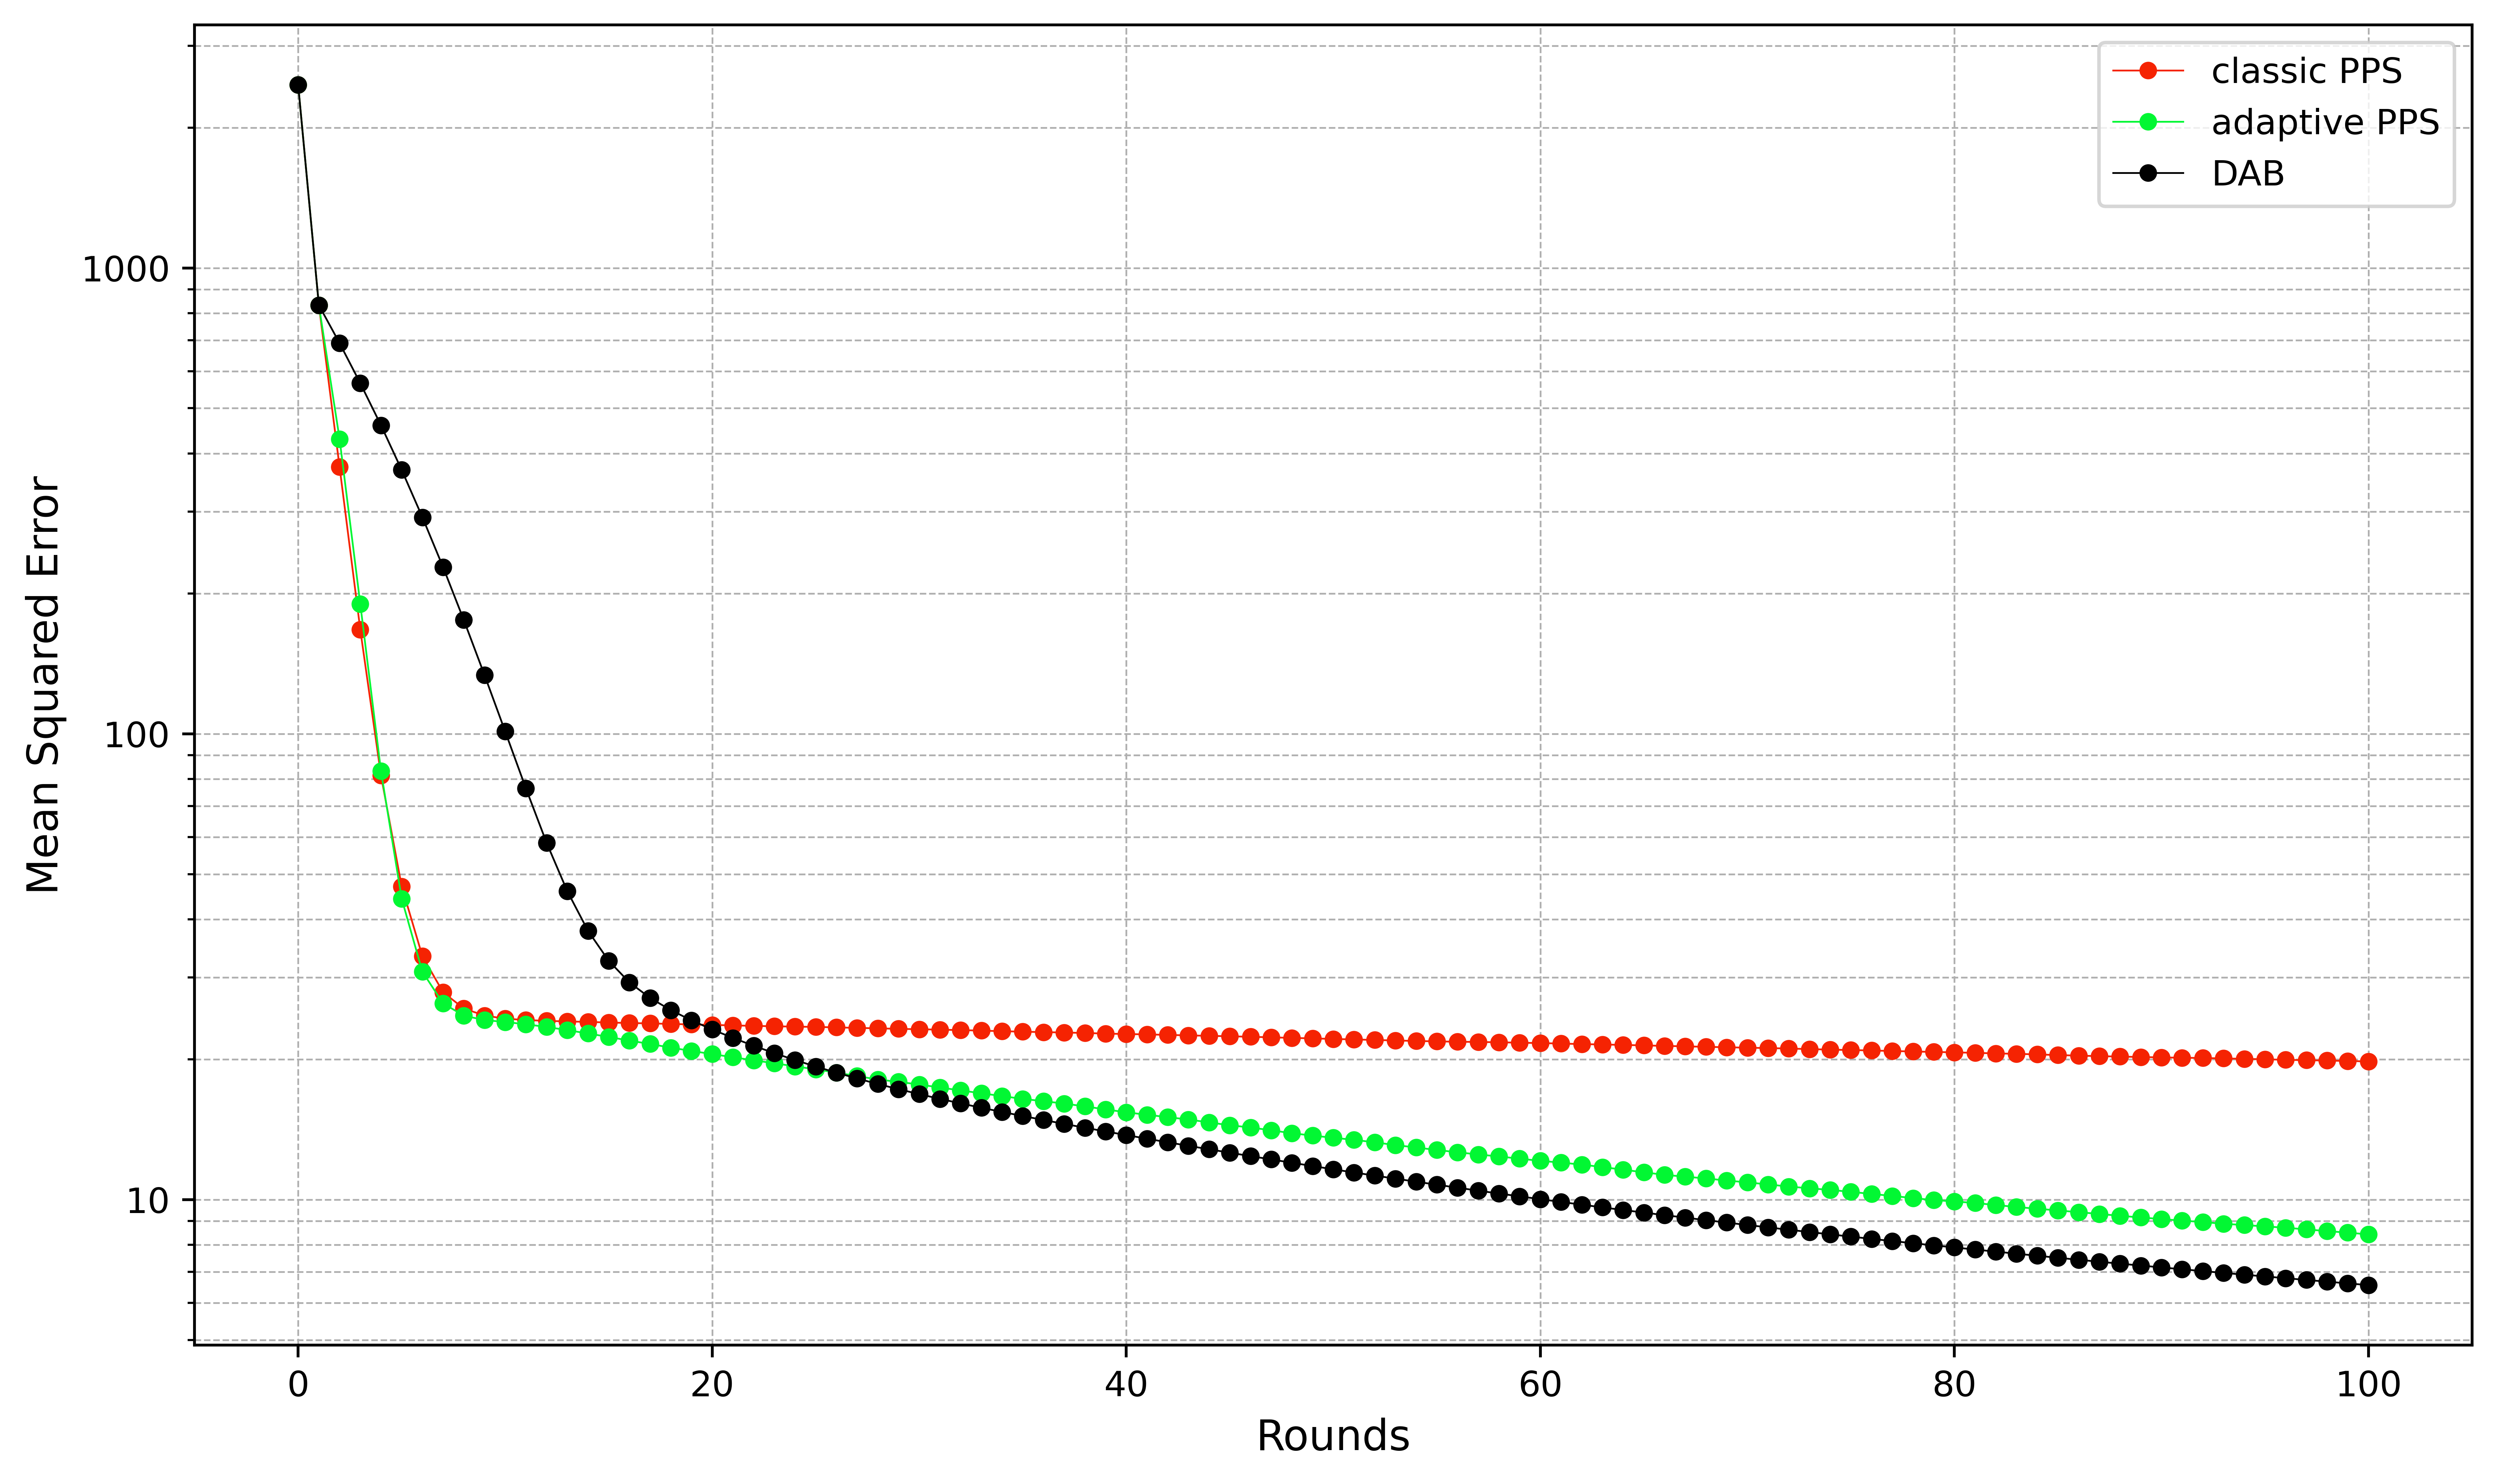
\includegraphics[width=0.49\linewidth]{figures/Simulation_outcomes/RingOfCliques/32x32/DAB_vs_PPS_RoC_r100_n1024_averaged_log.png}}
    \hfil
        \subfloat[]{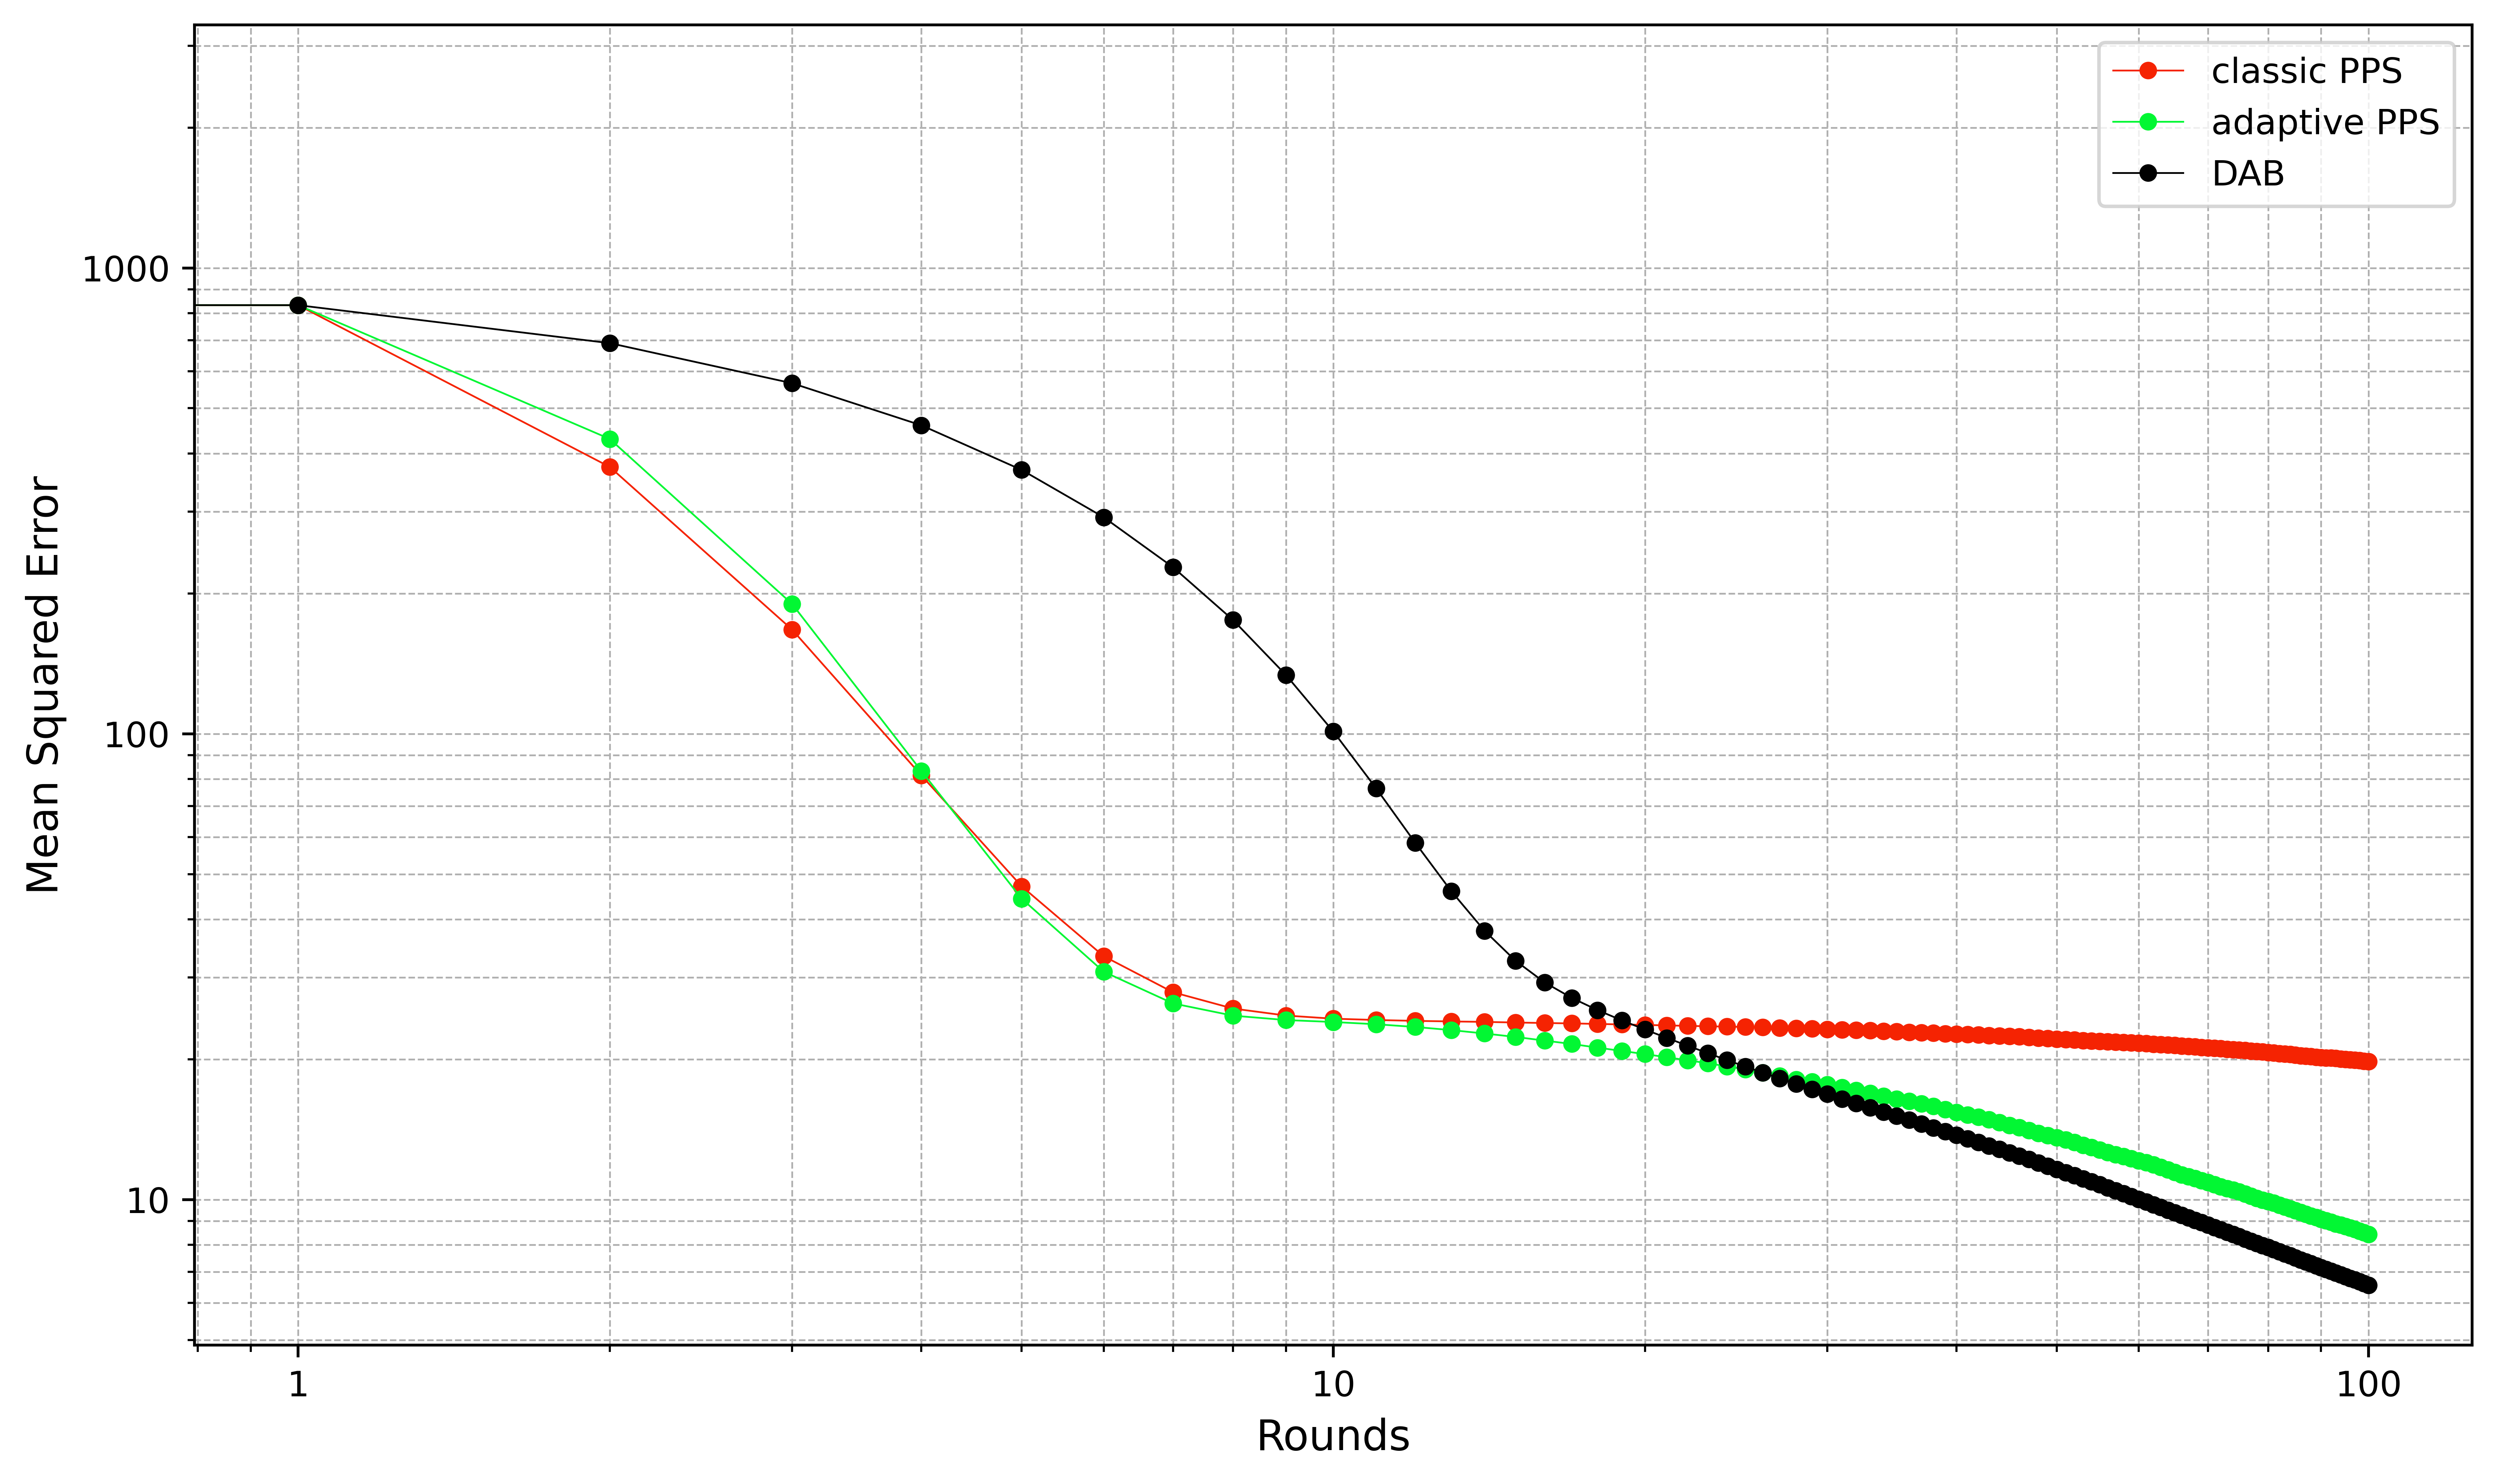
\includegraphics[width=0.49\linewidth]{figures/Simulation_outcomes/RingOfCliques/32x32/DAB_vs_PPS_RoC_r100_n1024_averaged_loglog.png}}
    \caption{$(32\times32)$-Ring of Cliques: mean squared error per rounds (log-linear and log-log)}
        \label{fig:atppsRingOfCliquesLog_LogLog}
\end{figure}
 \begin{figure}[]
     \centering
     \scalebox{0.8}{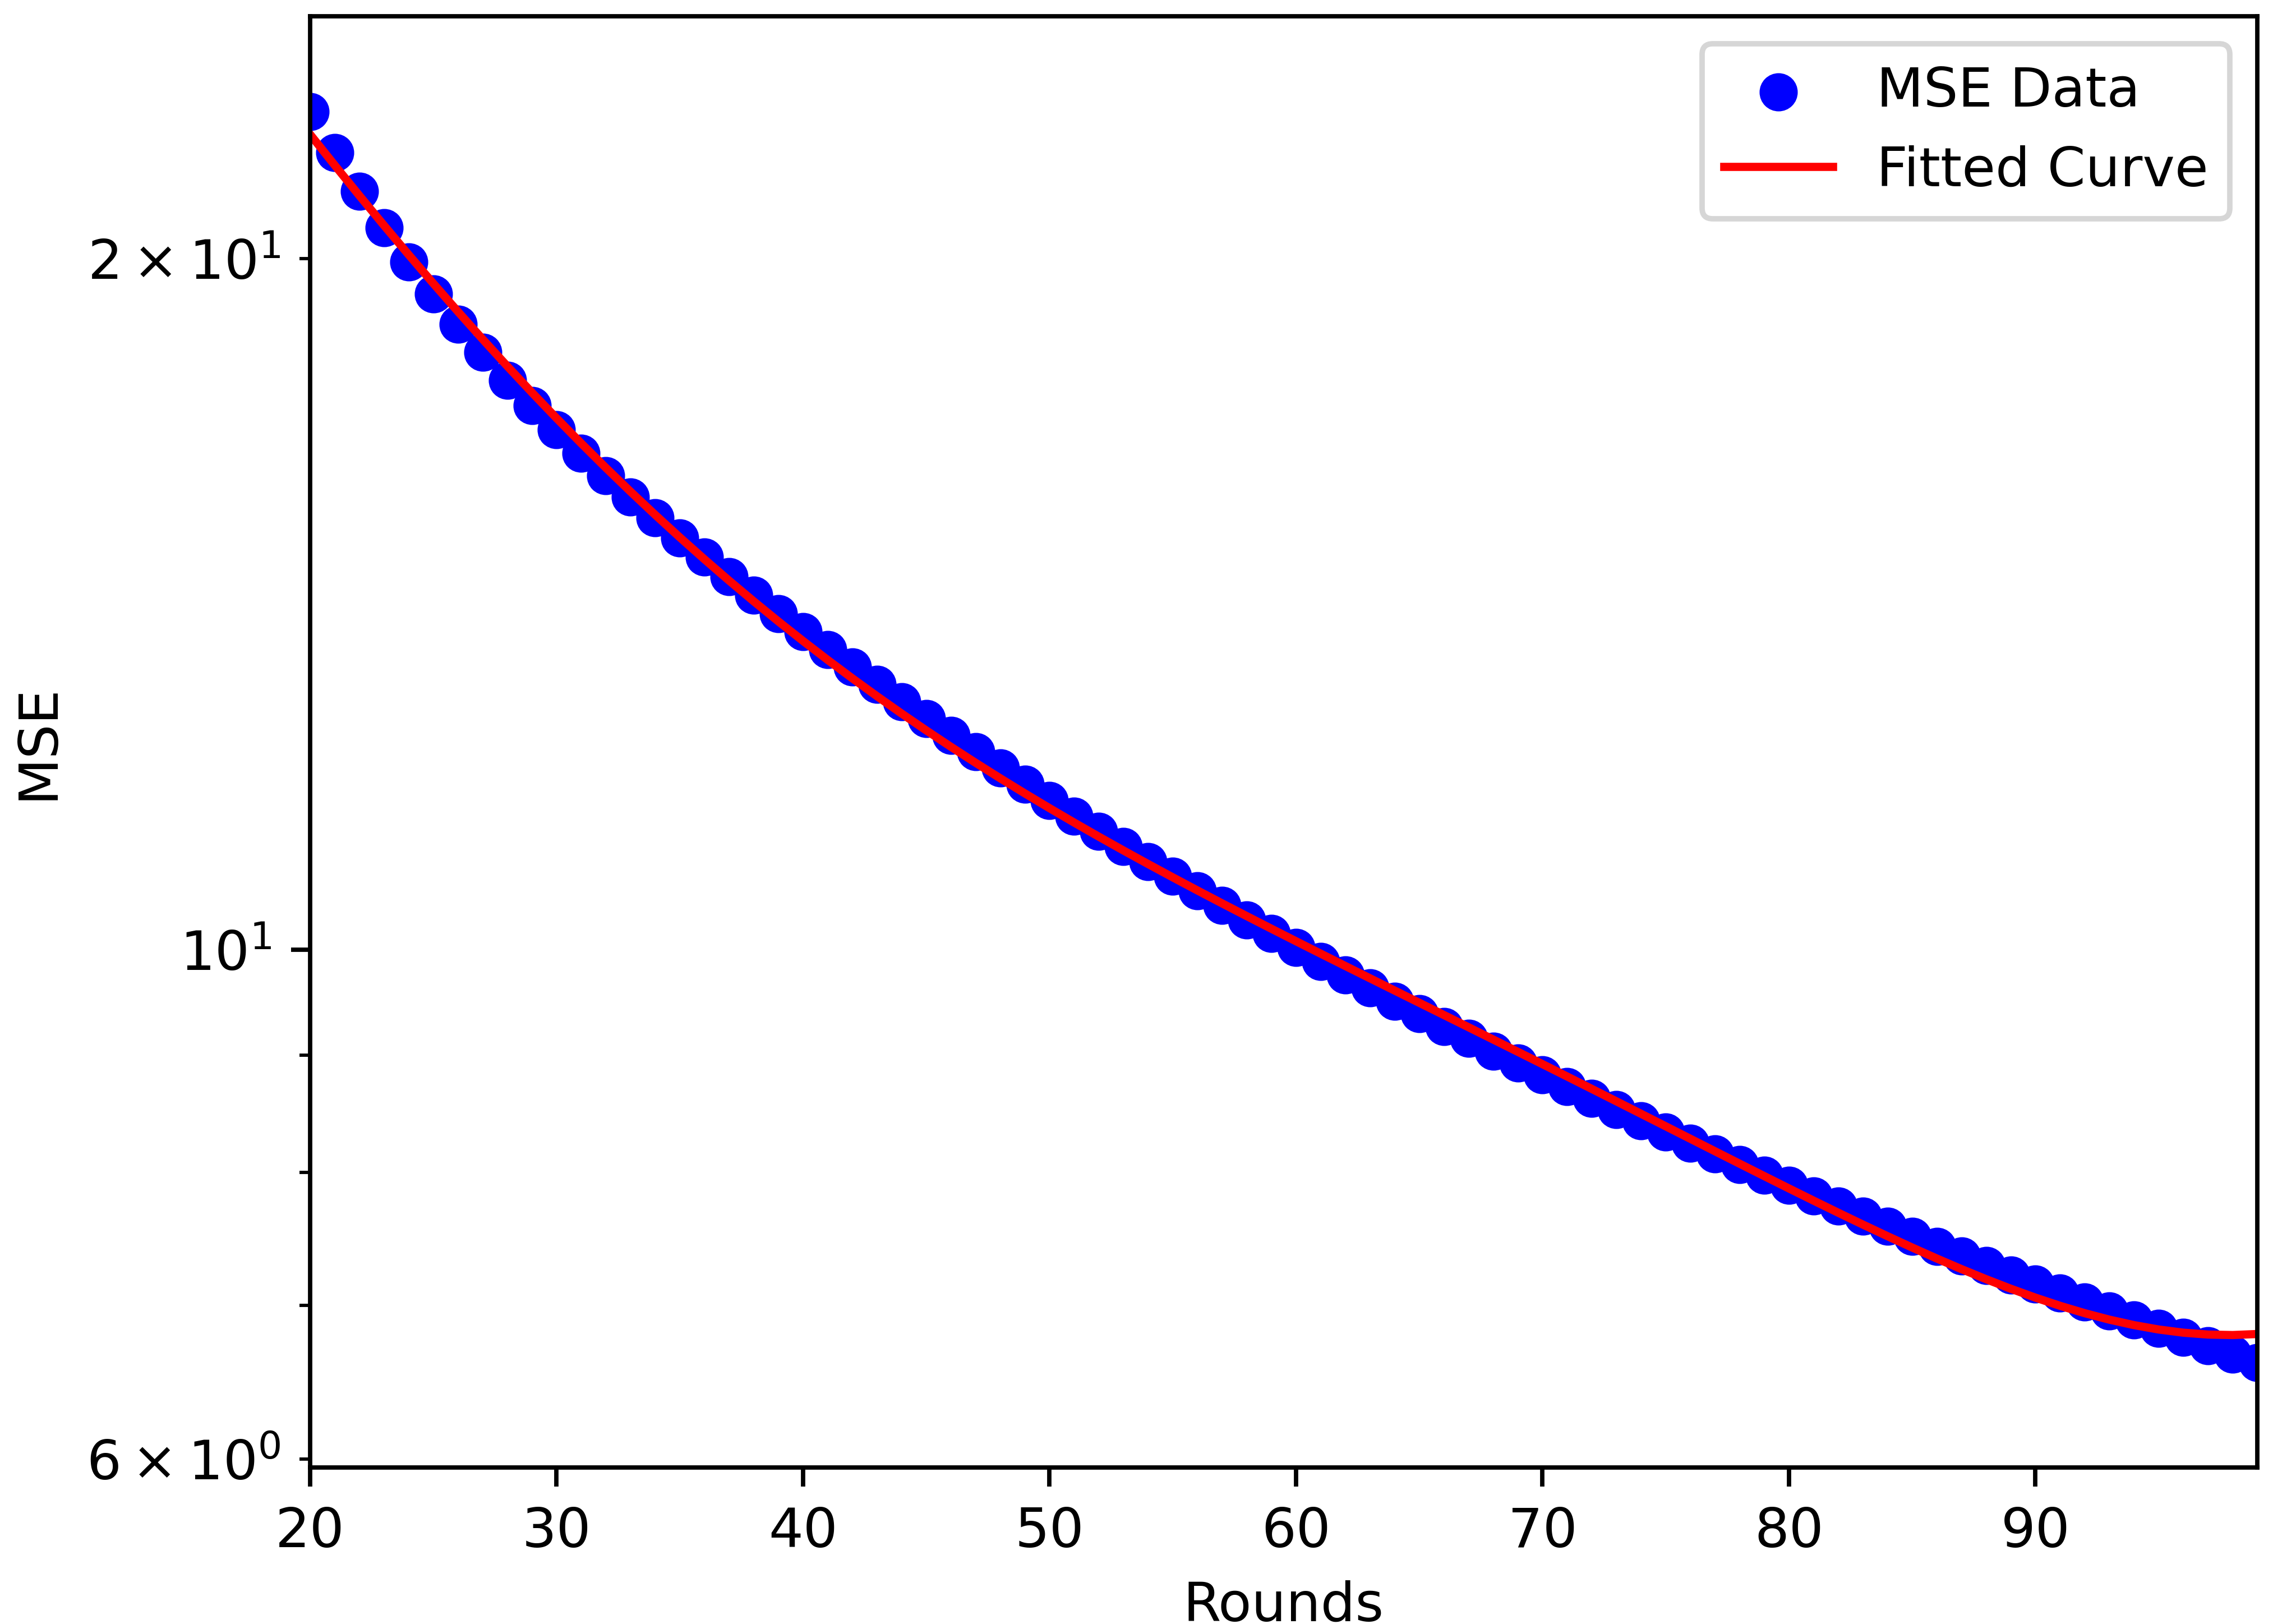
\includegraphics{figures/Simulation_outcomes/RingOfCliques/32x32/DAB/DAB_modelfitting_rounds_99_model_2.png}}
     \caption{$(32\times32)$-Ring of Cliques - polynomial regression fit: DAB}
     \label{fig:dabRingOfCliquesModelFit}
 \end{figure}
\begin{figure}[]
    \centering
    \scalebox{0.8}{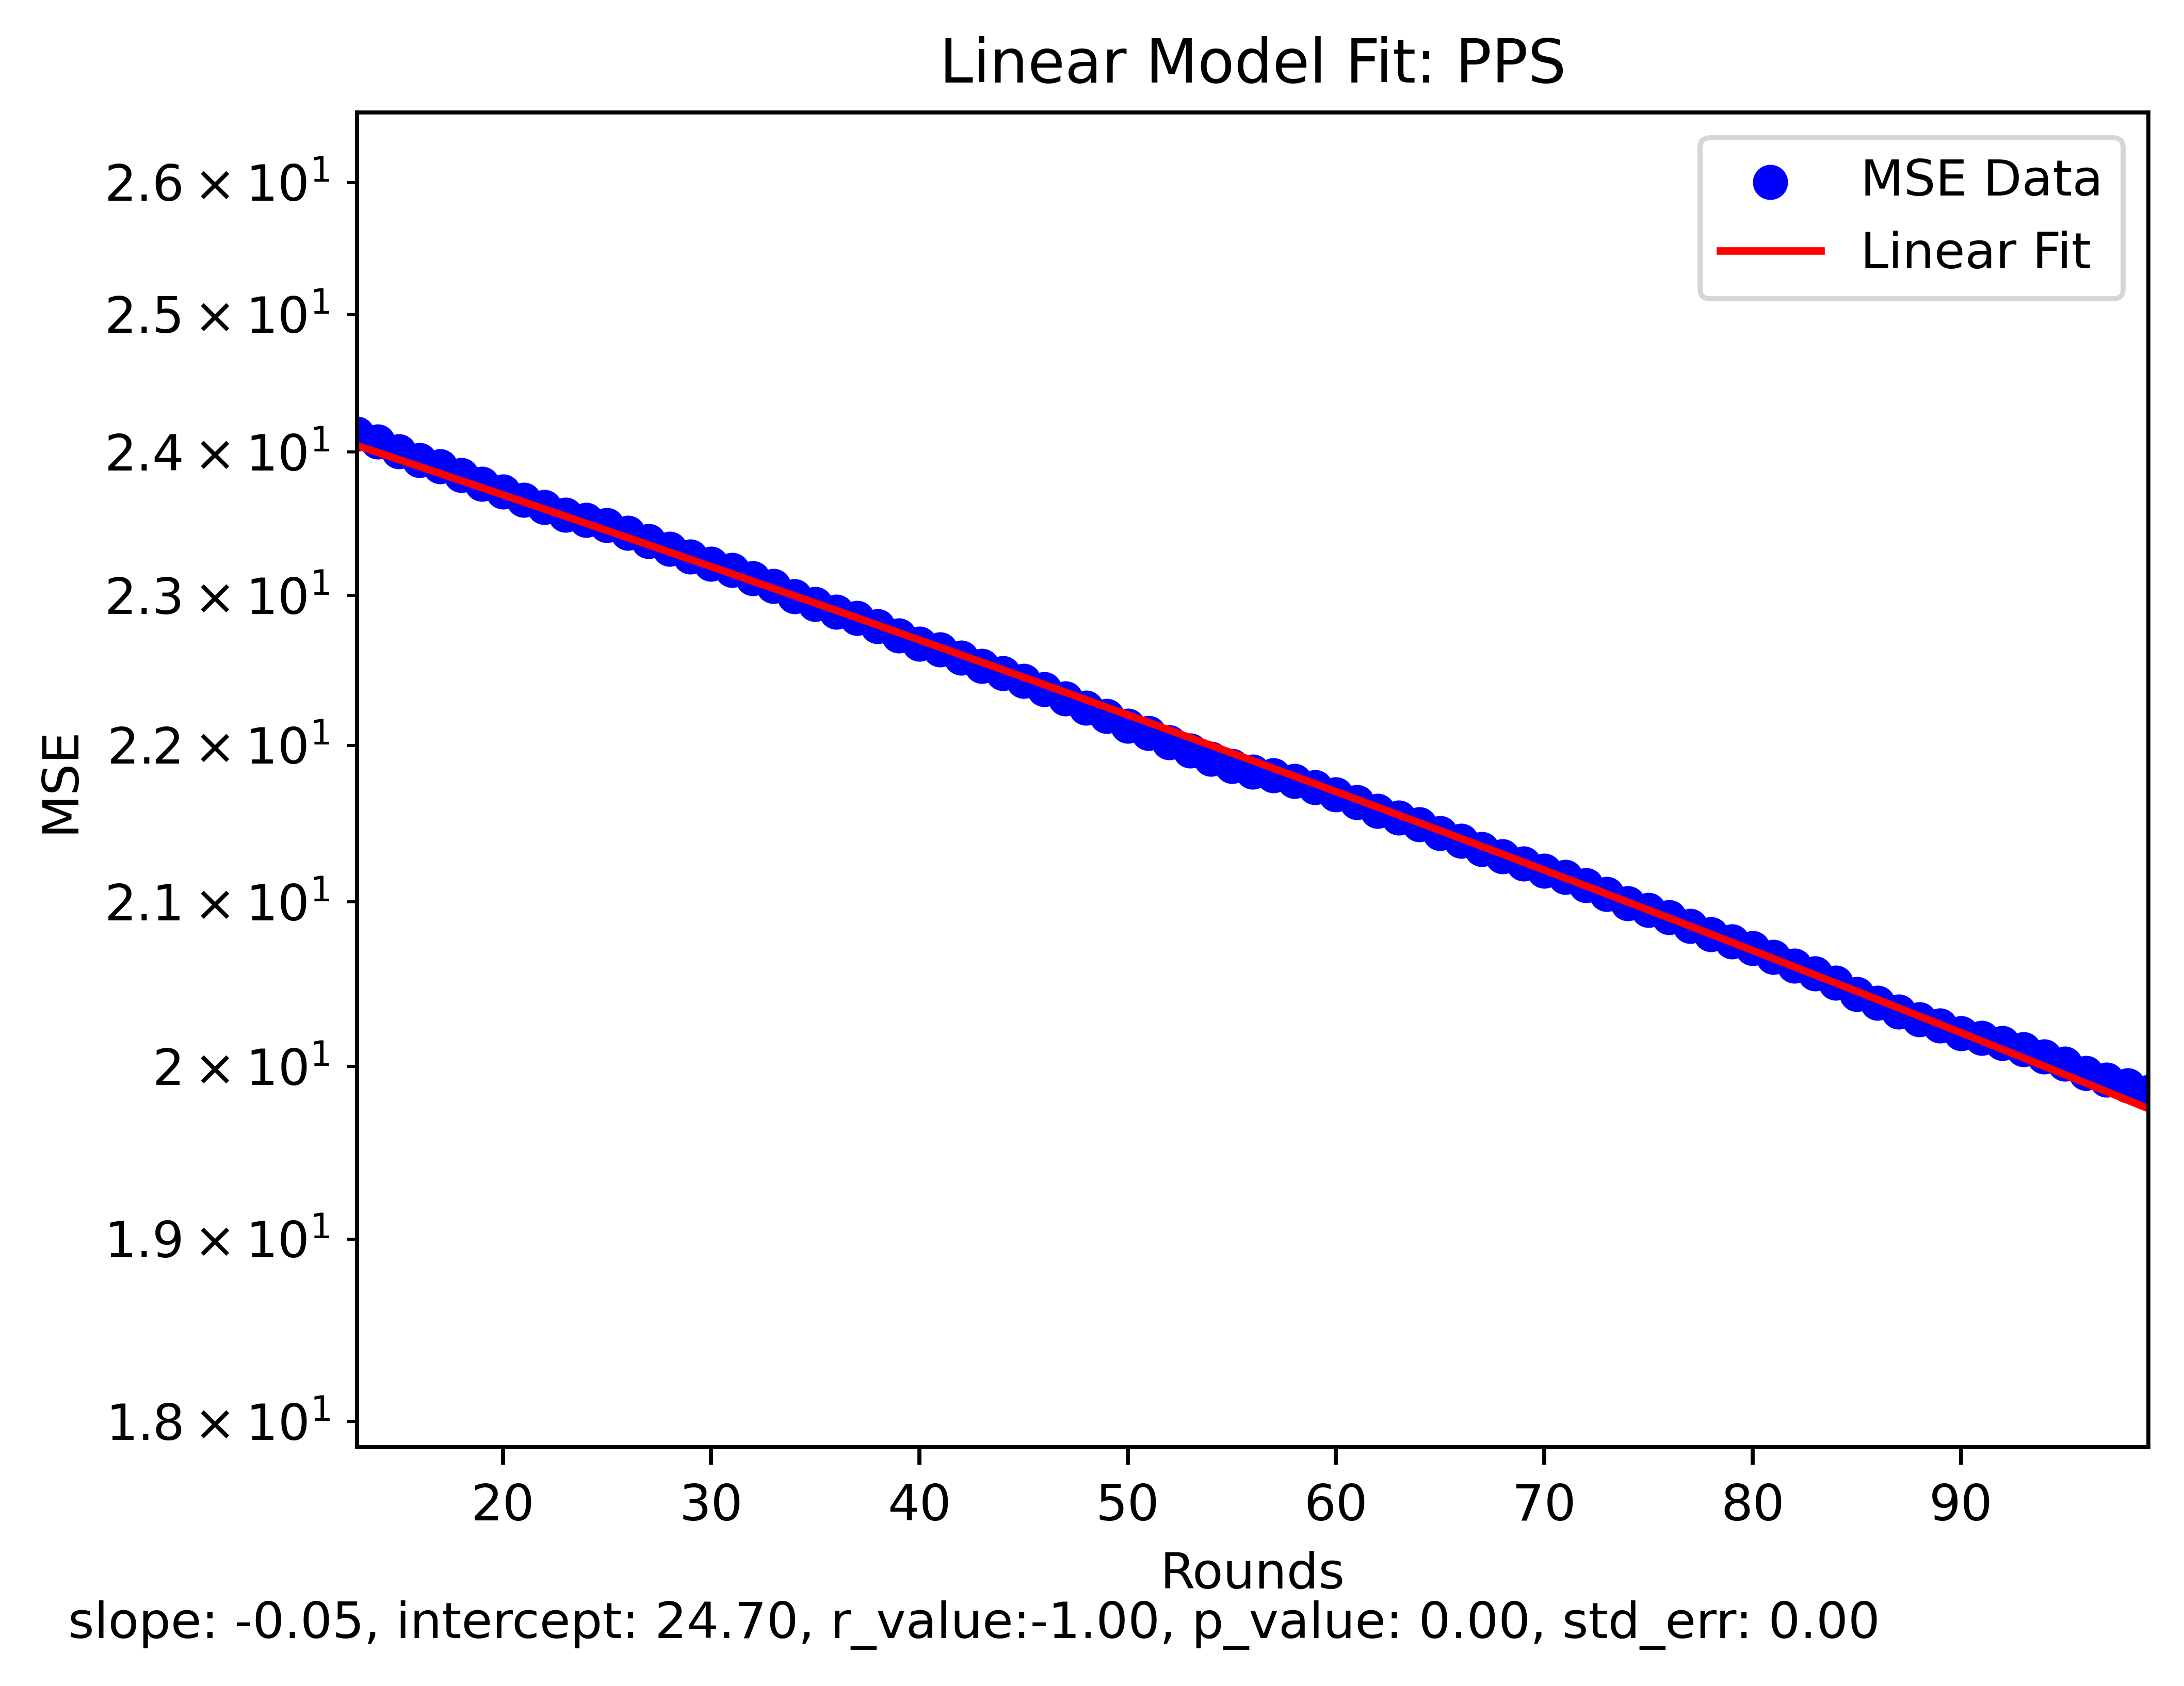
\includegraphics{figures/Simulation_outcomes/RingOfCliques/32x32/PPS/PPS_modelfitting_rounds_99_model_0.png}}
    \caption{$(32\times32)$-Ring of Cliques - polynomial regression fit: PPS}
    \label{fig:ppsRingOfCliquesModelFit}
\end{figure}

\begin{figure}[]
    \centering
    \scalebox{0.8}{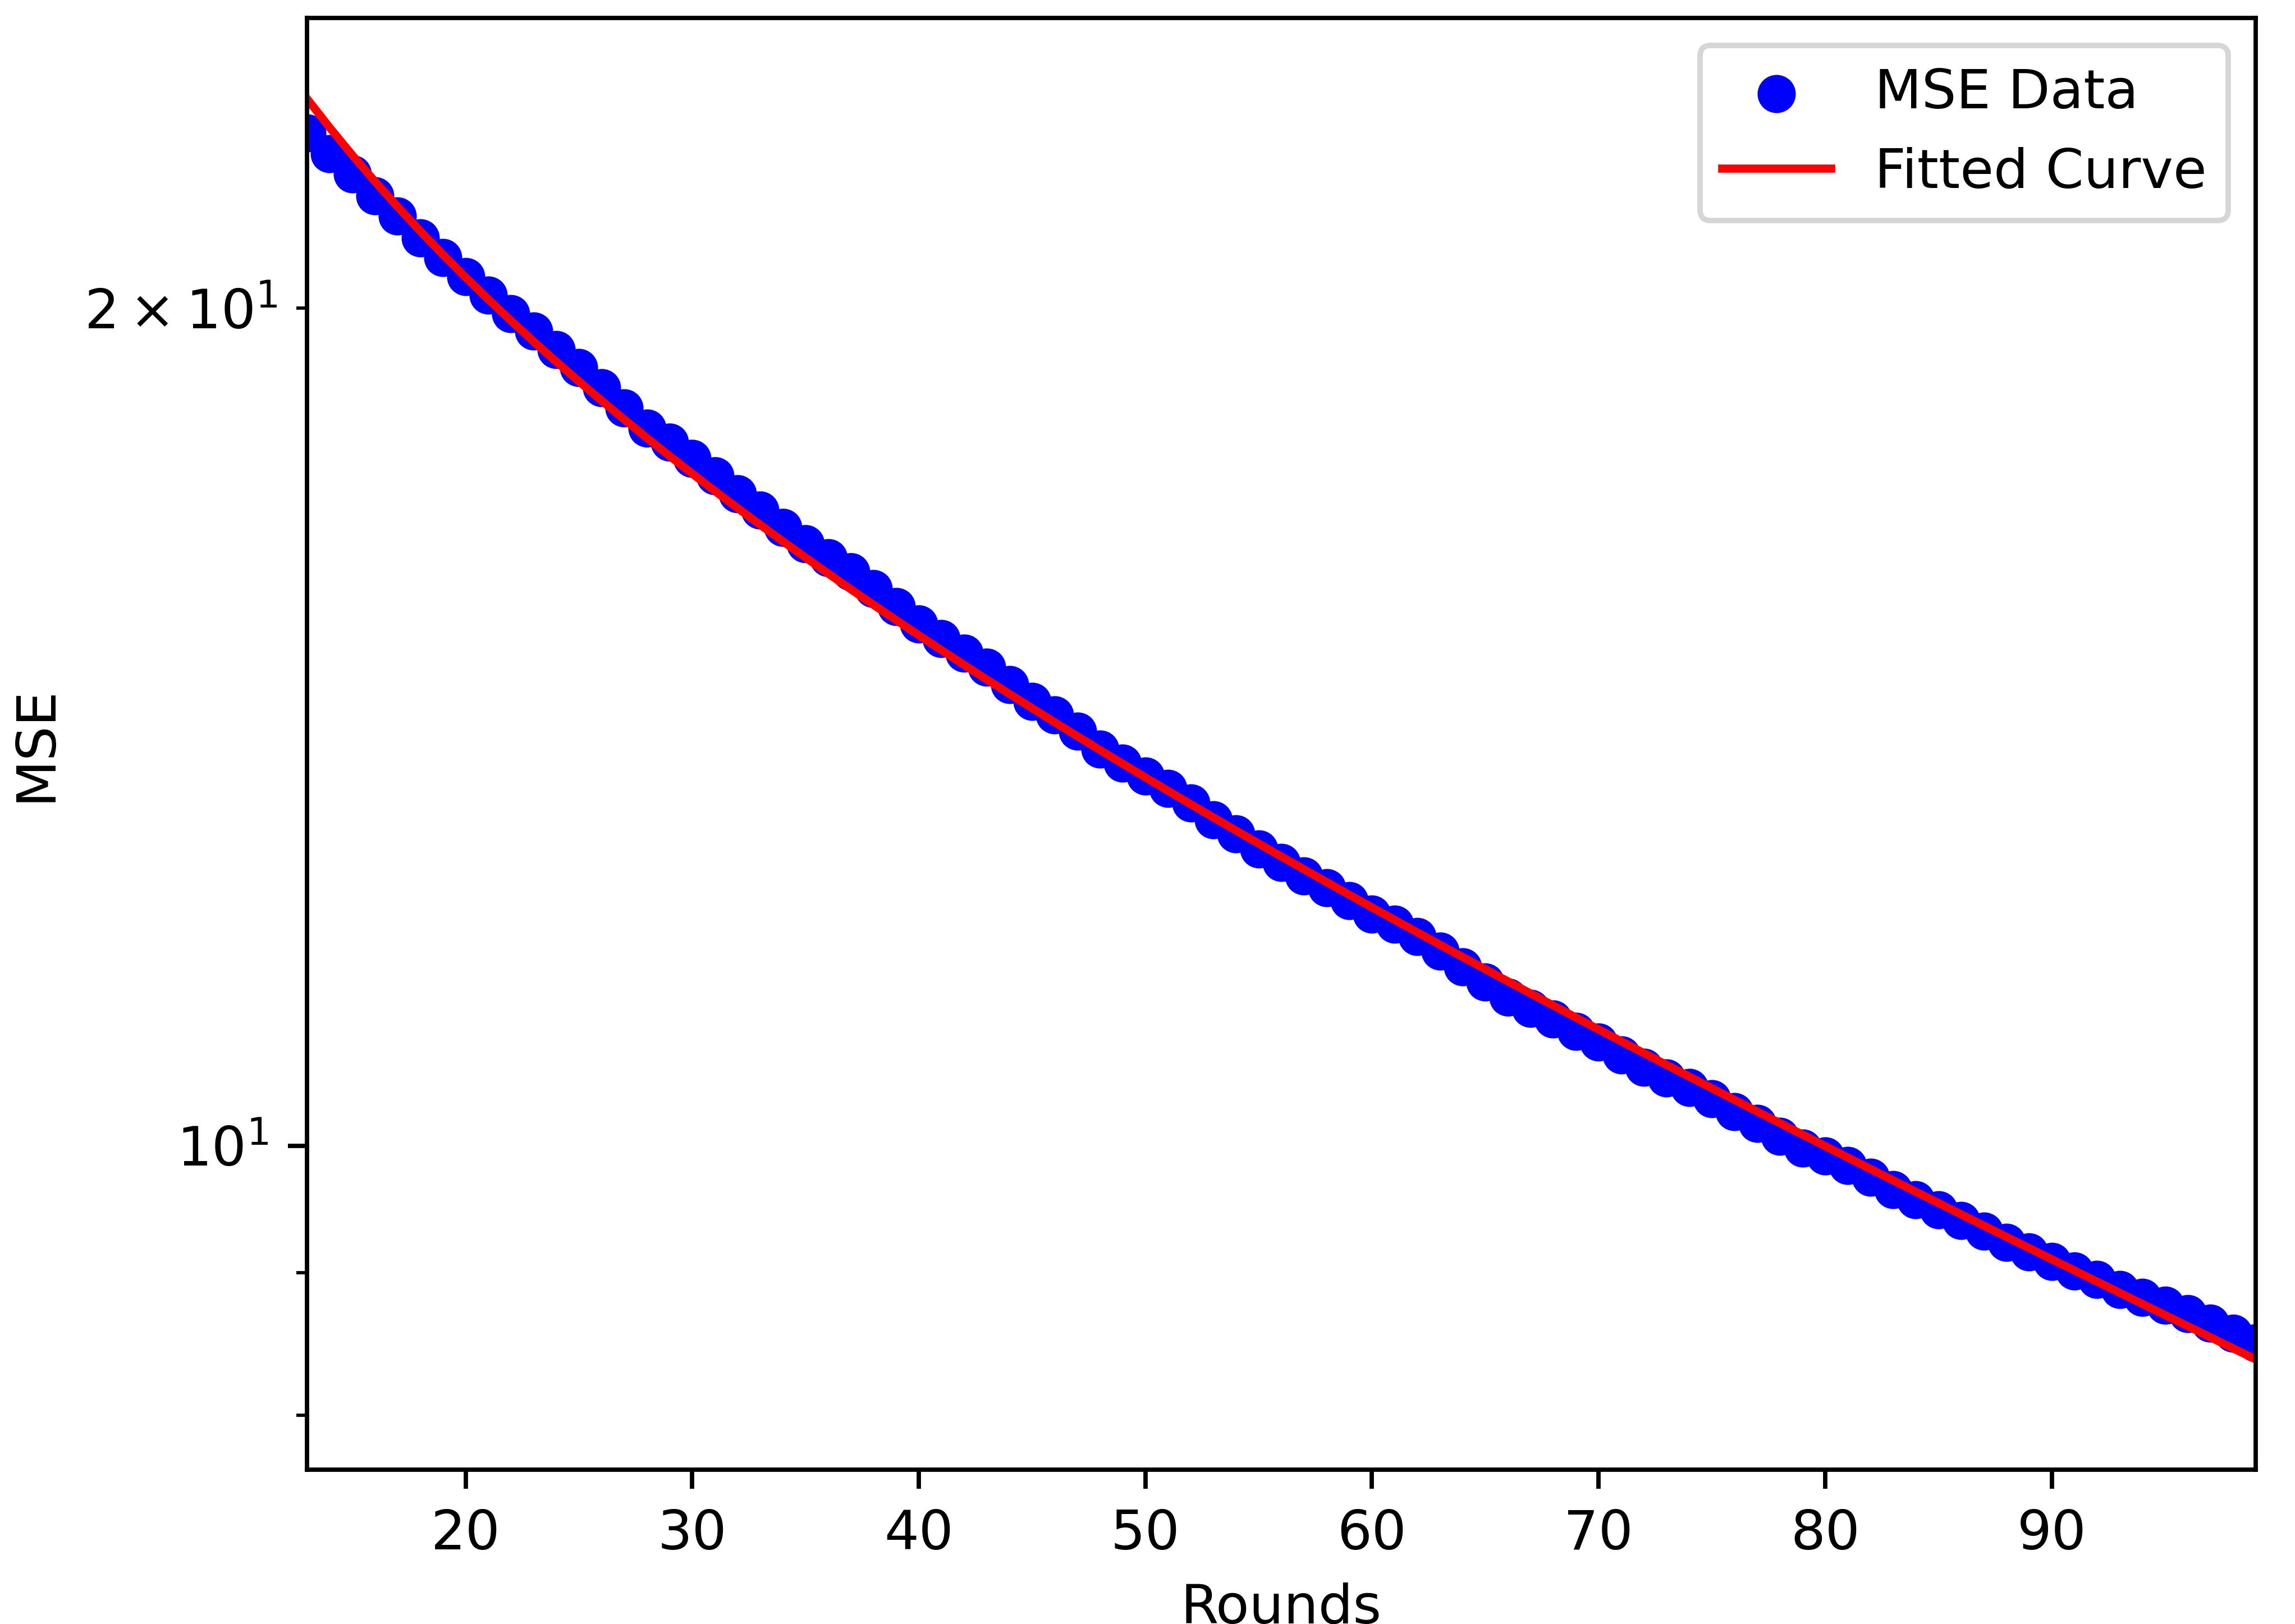
\includegraphics{figures/Simulation_outcomes/RingOfCliques/32x32/ATPPS/ATPPS_modelfitting_rounds_99_model_3.png}}
    \caption{$(32\times32)$-Ring of Cliques - logarithmic regression fit: ATPPS}
    \label{fig:atppsRingOfCliquesModelFit}
\end{figure}

\begin{figure}
    \centering
    \scalebox{0.8}{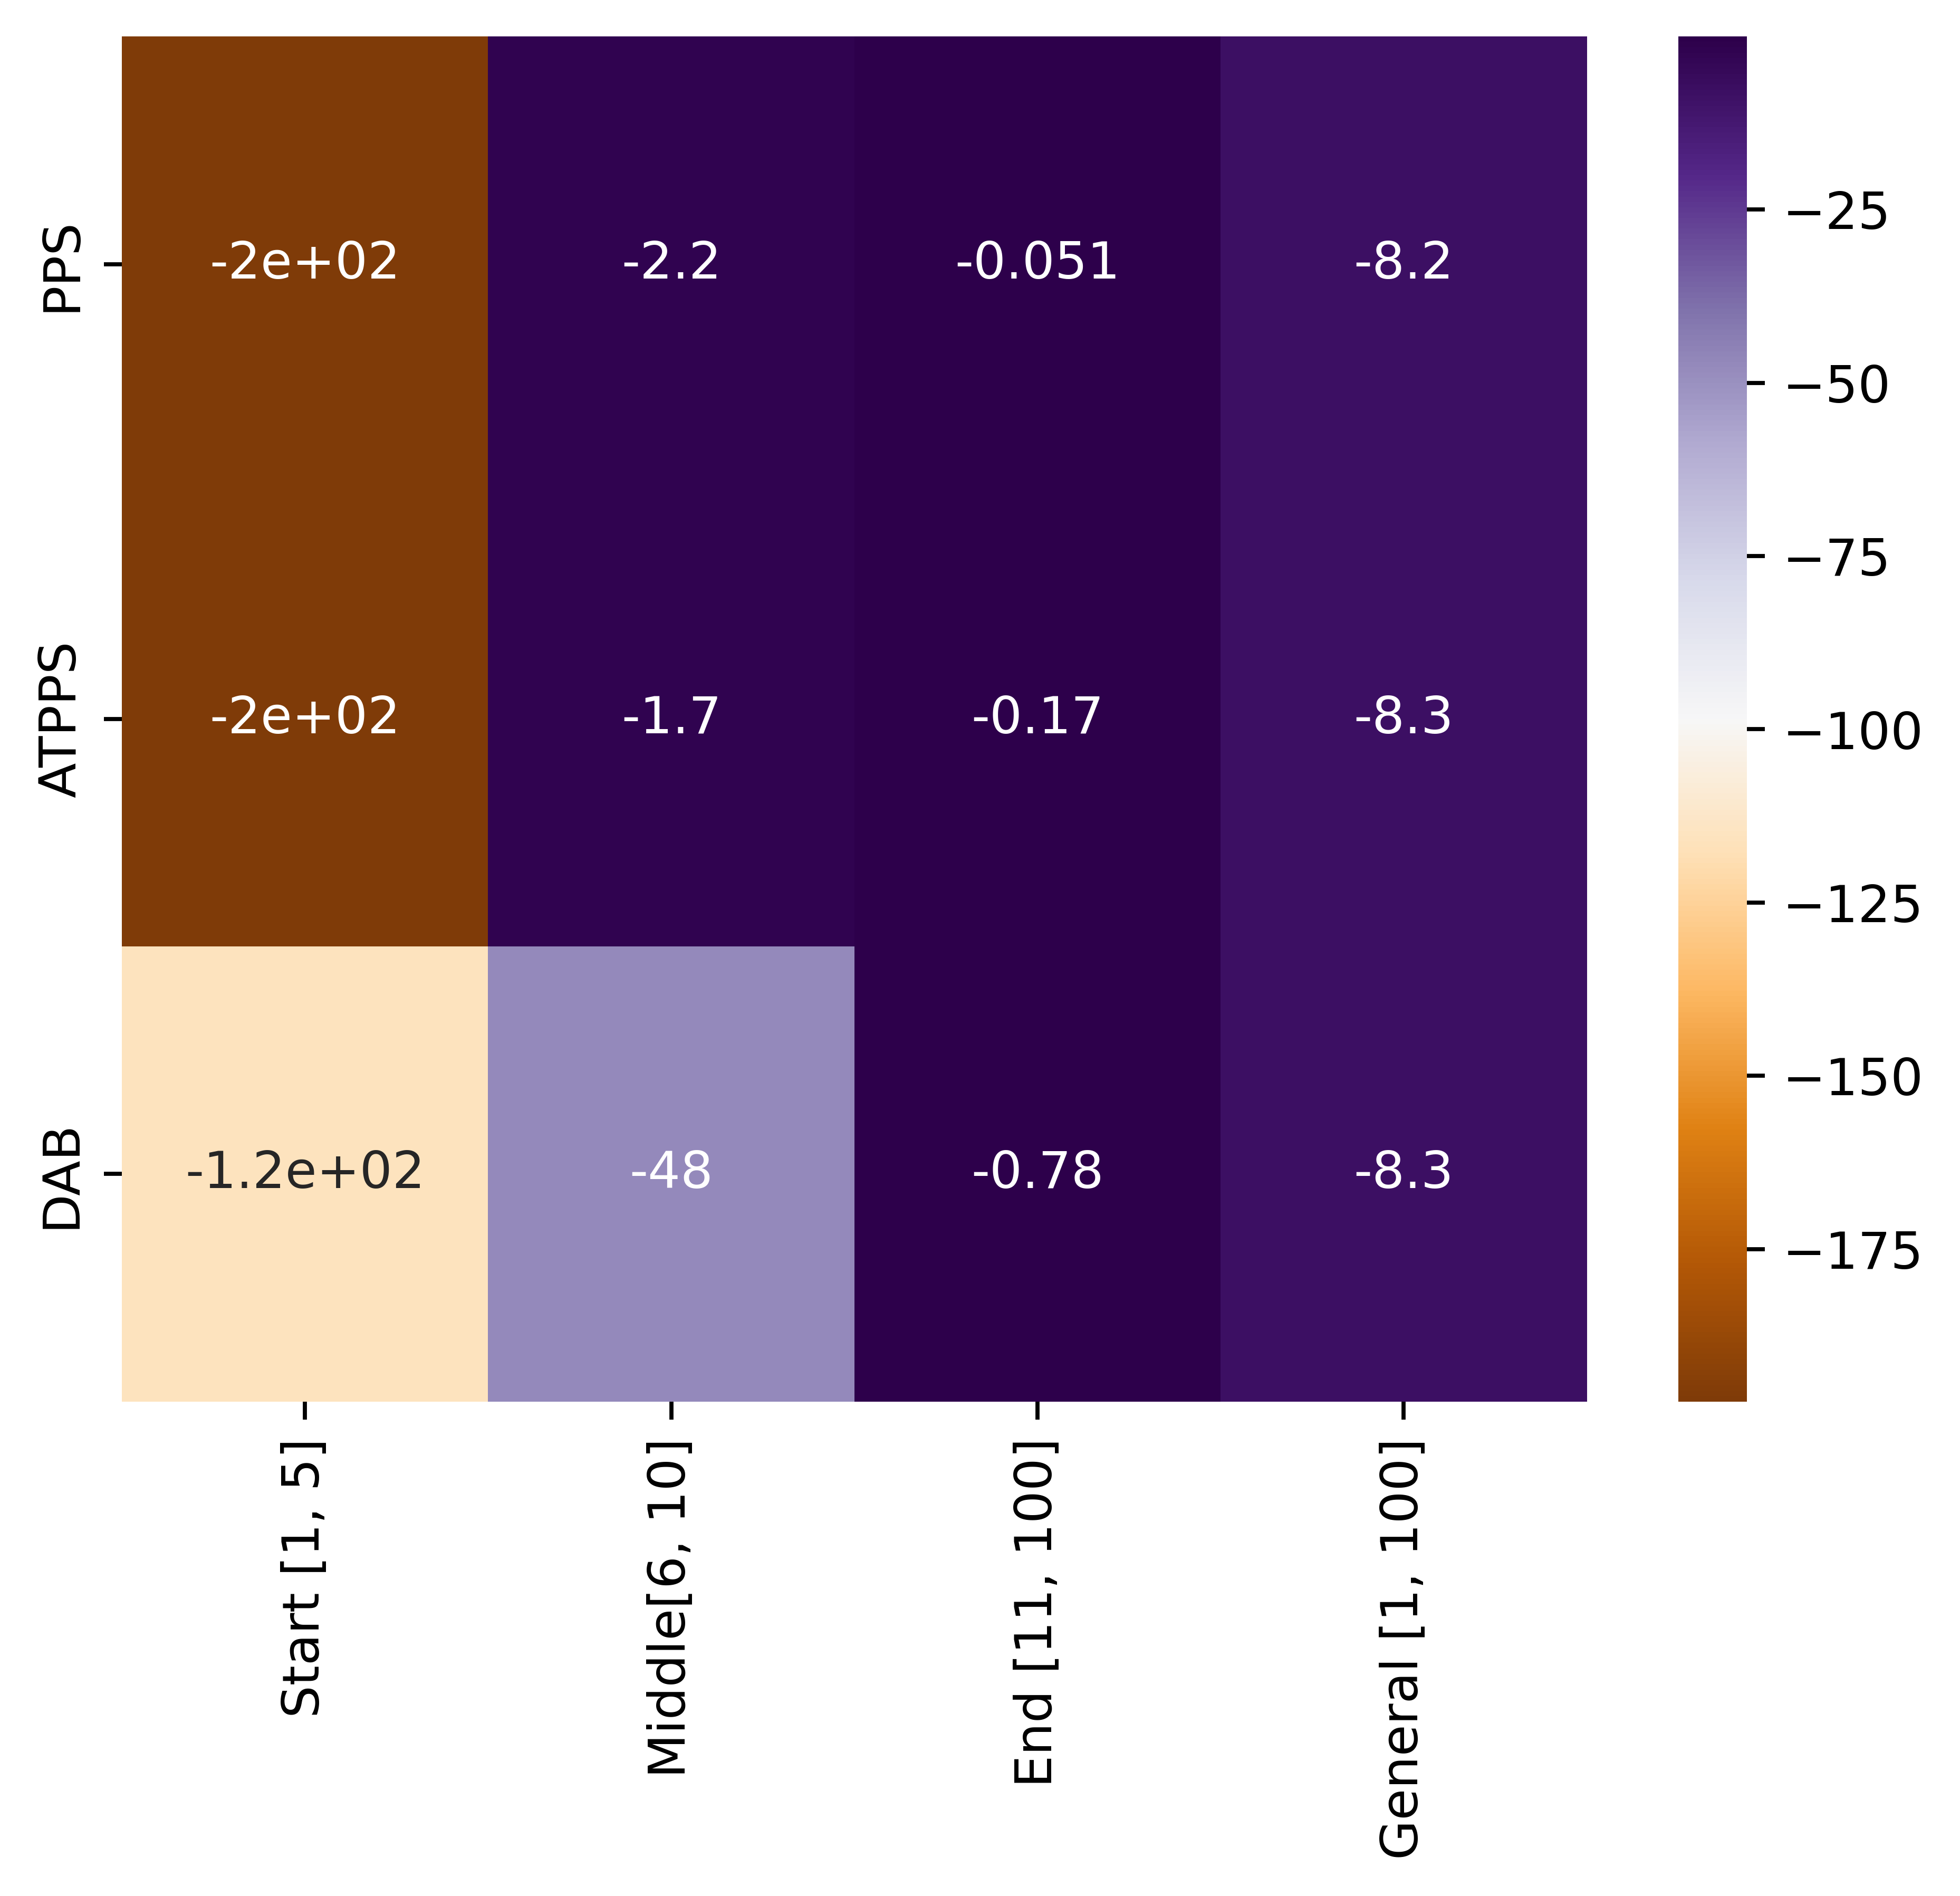
\includegraphics{figures/Simulation_outcomes/RingOfCliques/32x32/DAB_vs_PPS_vs_ATPPS_slopesheatmap_100rounds.png}}
    \caption{$(32\times32)$-Ring of Cliques: heat map of slopes per region}
    \label{fig:ringOfCliquesslopes}
\end{figure}

In the following the Ring of Cliques are newly organized. Experiments are conducted where the number of cliques is increased from $2^{5}$ to $2^{7}$ in subsection \ref{subsec:128_8ROC} and thus the clique size of each clique is decreased to $2^{3}$. Subsection \ref{subsec:8_128ROC} covers the experiment where the clique size is increased and the number of cliques is decreased in the same magnitude as discussed before.

\subsection{128x8 Ring of Cliques}\label{subsec:128_8ROC}
The clique size plays a crucial role for the efficacy of the DAB algorithm. The decreased clique size favors the DAB making it the load balancing algorithm to reduce the error in the network more rapidly than the Push-Pull Sum based algorithms as seen in figure \ref{fig:128x8RingOfCliquesLog_LogLog}. All the load balancing algorithms show an rapid decrease of error in the network, indicated by the steep negative slopes as visualized in figure \ref{fig:128x8ringOfCliquesslopes}. The Push-Pull Sum based algorithms show an decrease of -180, whereas the DAB shows a decrease of -190 in the start region (rounds 1 to 5). After the very steep decrease in the start region the load balancing algorithms decrease the error more moderately, where the DAB algorithm still has the steepest decrease of error of -5.2, followed by the ATPPS decreasing the error as low as -4.6, lastly the PPS follows with a slope of -3.6. The curve in this region is rather flat as seen in the log-log representation in figure \ref{fig:128x8RingOfCliquesLog_LogLog} a) The decrease effect diminishes as the error of the network is already relatively low, in the end region. The MSE values at the end of round of 100 show the magnitude of error reduction. The DAB scored the lowest MSE value 10.64, followed by the ATPPS achieving very good results to with a MSE value of 13.68. The PPS value achieved the highest MSE value of 22.33. Compared to the $(32\times 32)$-Ring of Cliques the load balancing algorithms reduced the error even more by a margin of 2 to 4 units. The most improvement is drawn by the ATPPS with a lower value of around around 5 followed by the DAB, with a lower MSE of 4 and lastly the PPS with a decreased value of around 2.

All three load balancing algorithms were fitted against polynomials with degree 4. The equations are as follows: DAB $MSE_r=5.45\times 10 ^{-7}r^{4}-1.7\times 10^{-4}r^{3}+0.02r^{2}-1.33r+46.71$ (figure \ref{fig:128x8dabRingOfCliquesModelFit}) PPS: $MSE_r=1.04\times 10 ^{-6}r^{4}-3.41\times 10^{-4}r^{3}+0.04r^{2}-2.73r+97.58$ (figure \ref{fig:128x8ppsRingOfCliquesModelFit}) and ATPPS: $MSE_r=9.54\times 10^{-7}r^{4}-2.93\times 10^{-4}r^{3}+0.03r^{2}-2.05r+67.02$ (figure \ref{fig:128x8atppsRingOfCliquesModelFit}).
\begin{figure}[!ht]
    \centering
        \subfloat[]{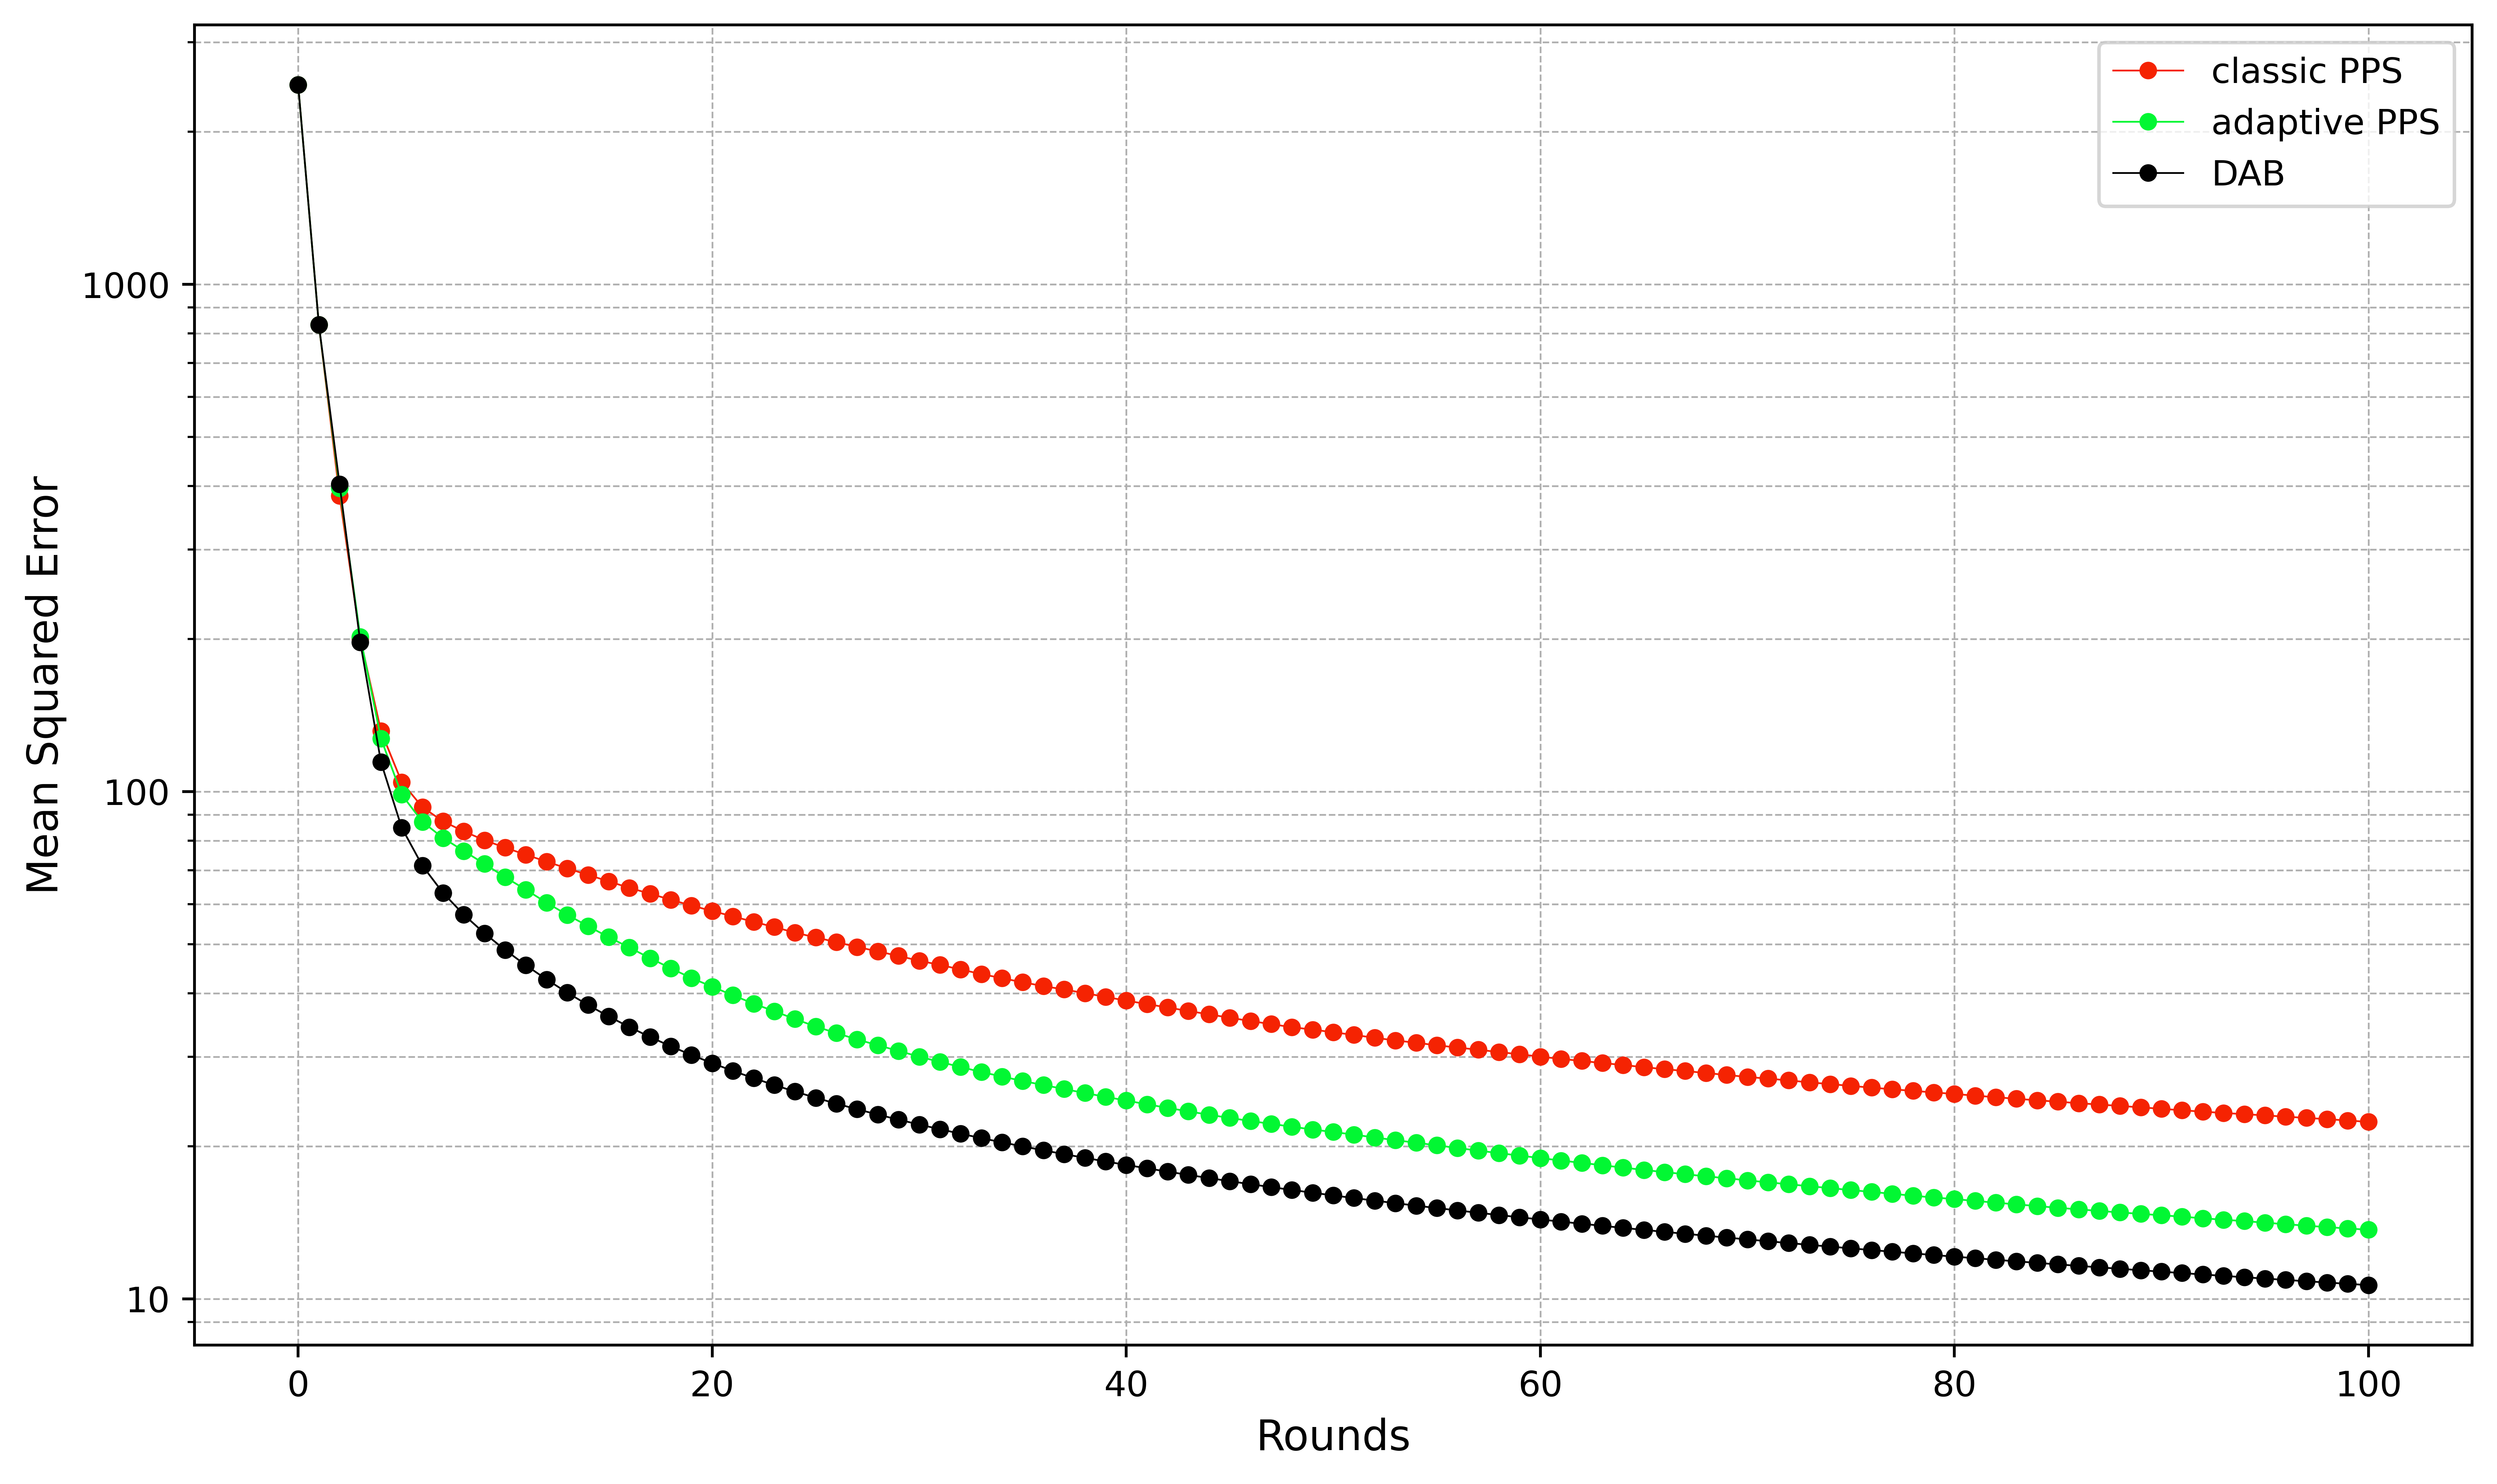
\includegraphics[width=0.49\linewidth]{figures/Simulation_outcomes/RingOfCliques/128x8/DAB_vs_PPS_RoC_r100_n1024_averaged_log.png}}
    \hfil
        \subfloat[]{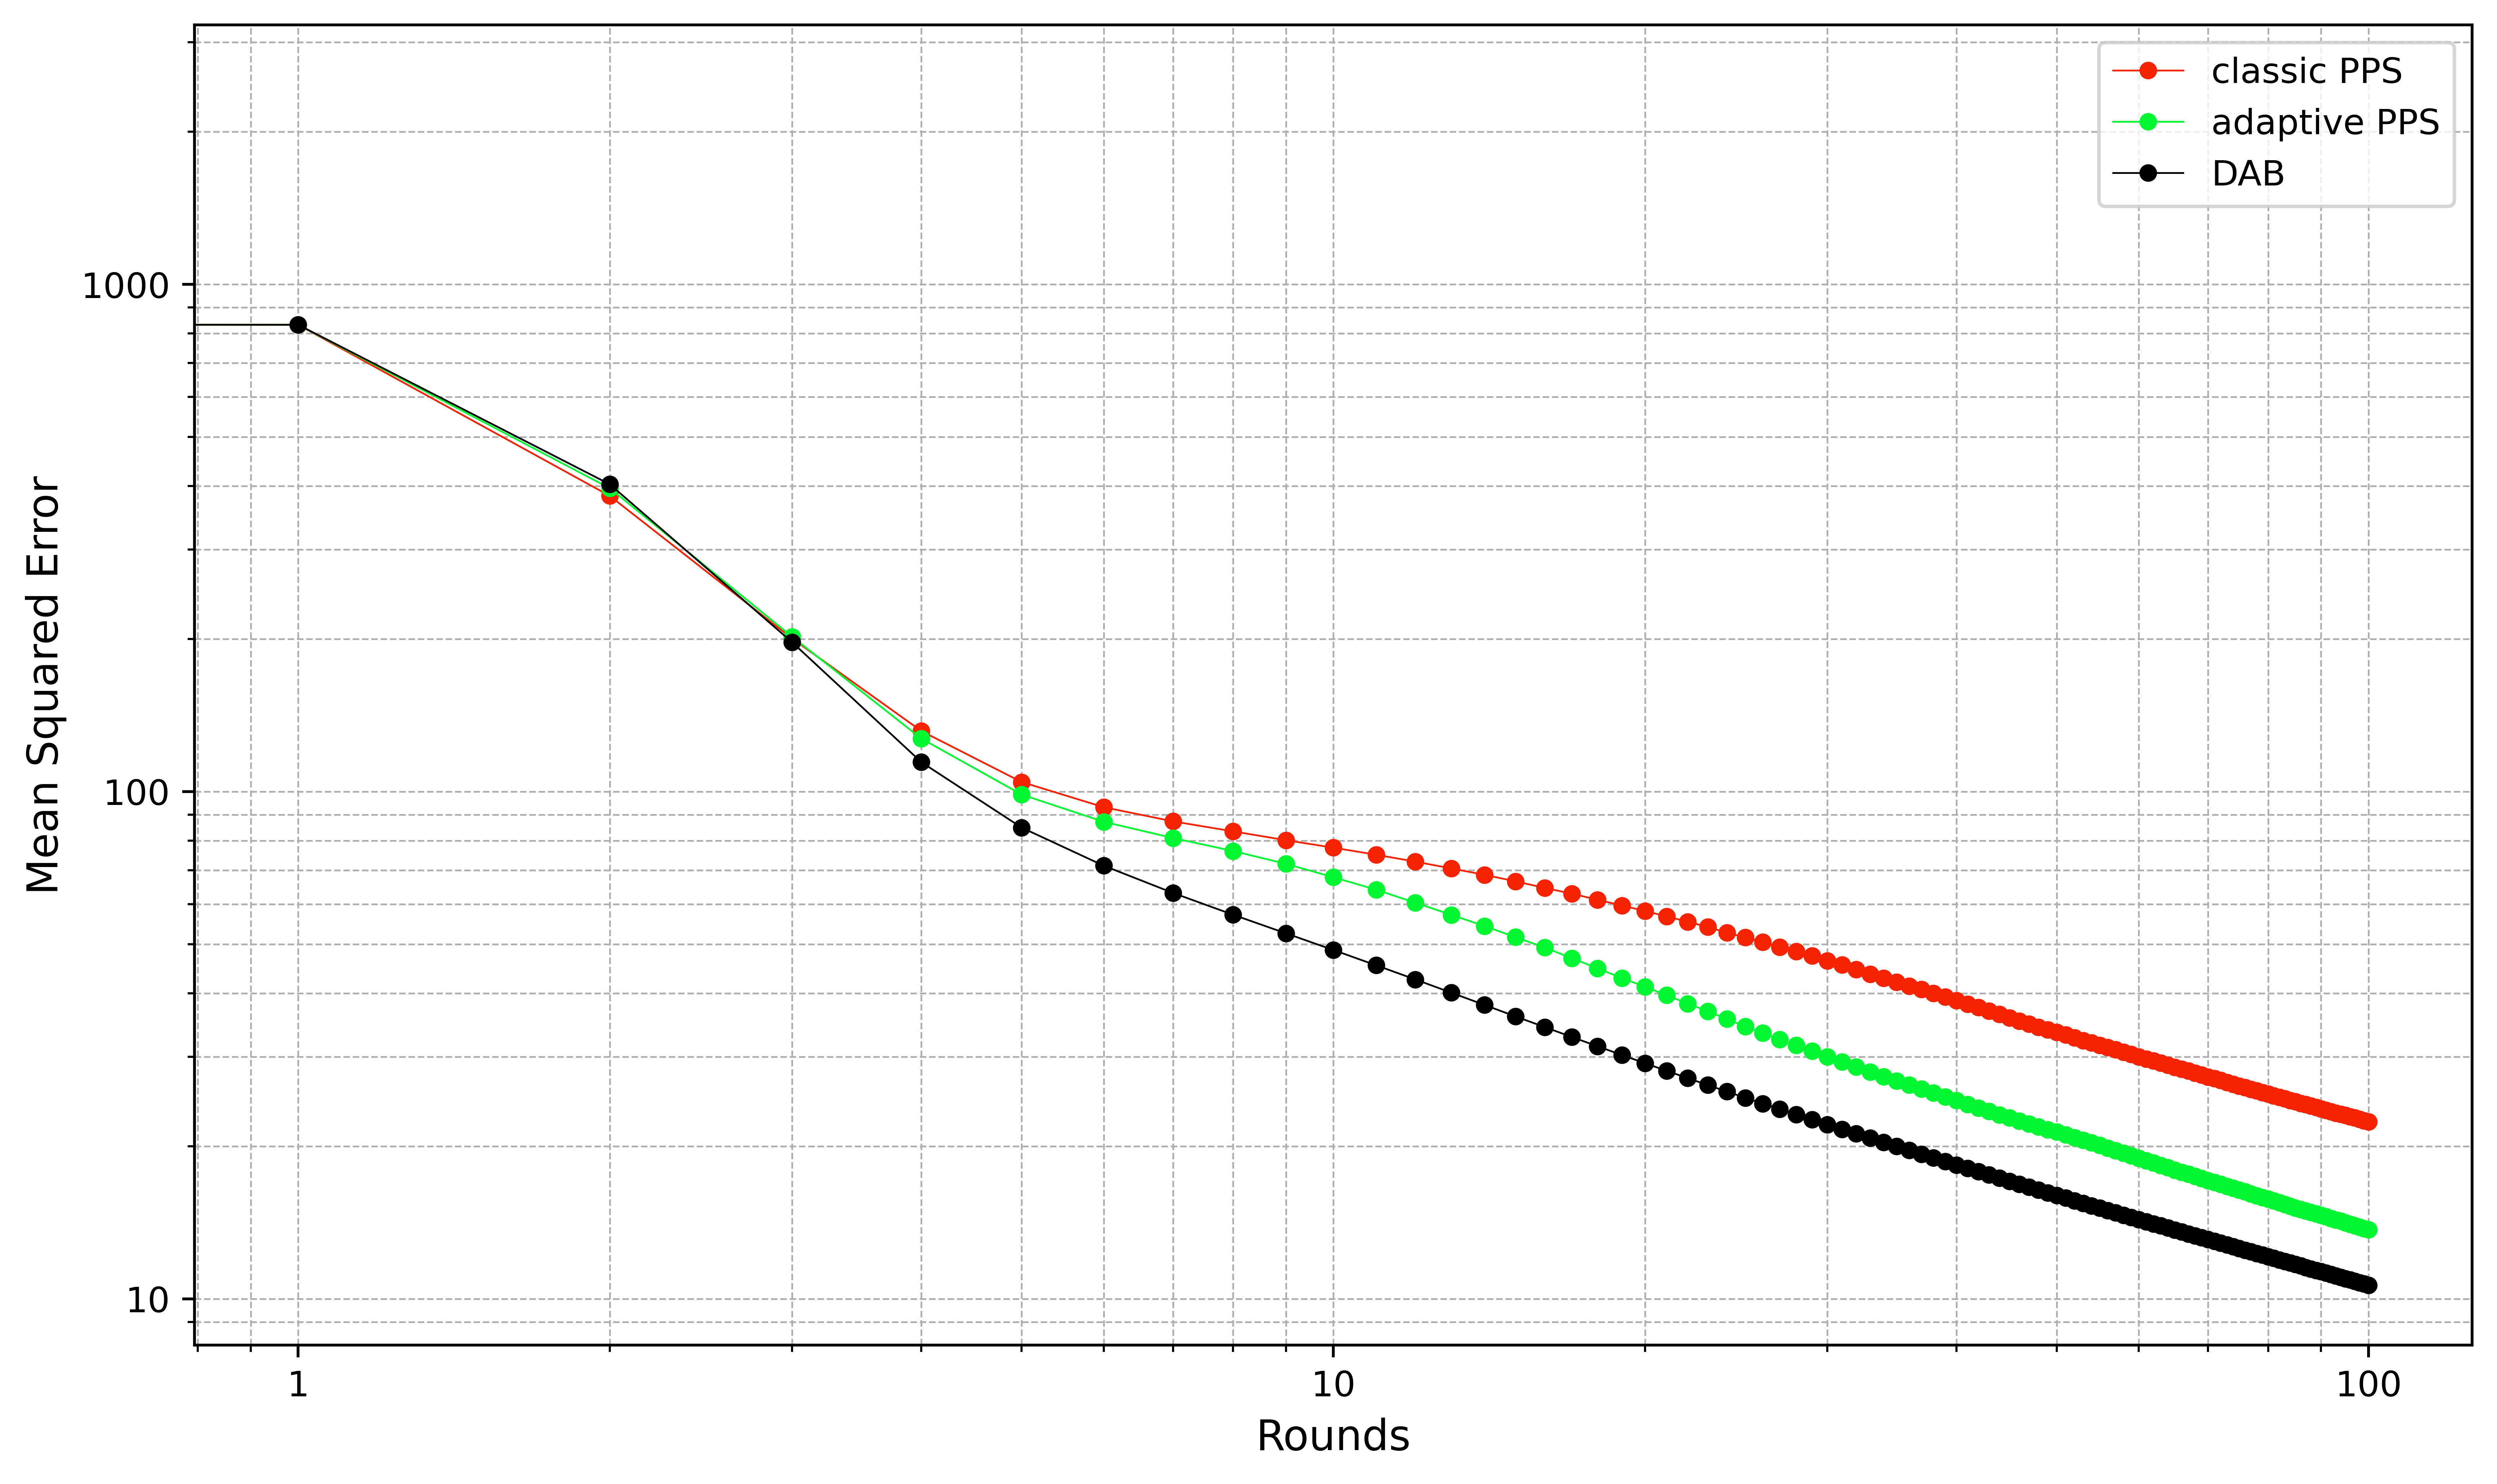
\includegraphics[width=0.49\linewidth]{figures/Simulation_outcomes/RingOfCliques/128x8/DAB_vs_PPS_RoC_r100_n1024_averaged_loglog.png}}
    \caption{$(128\times8)$-Ring of Cliques: mean squared error per rounds (log-linear and log-log)}
        \label{fig:128x8RingOfCliquesLog_LogLog}
\end{figure}

\begin{figure}[]
     \centering
     \scalebox{0.8}{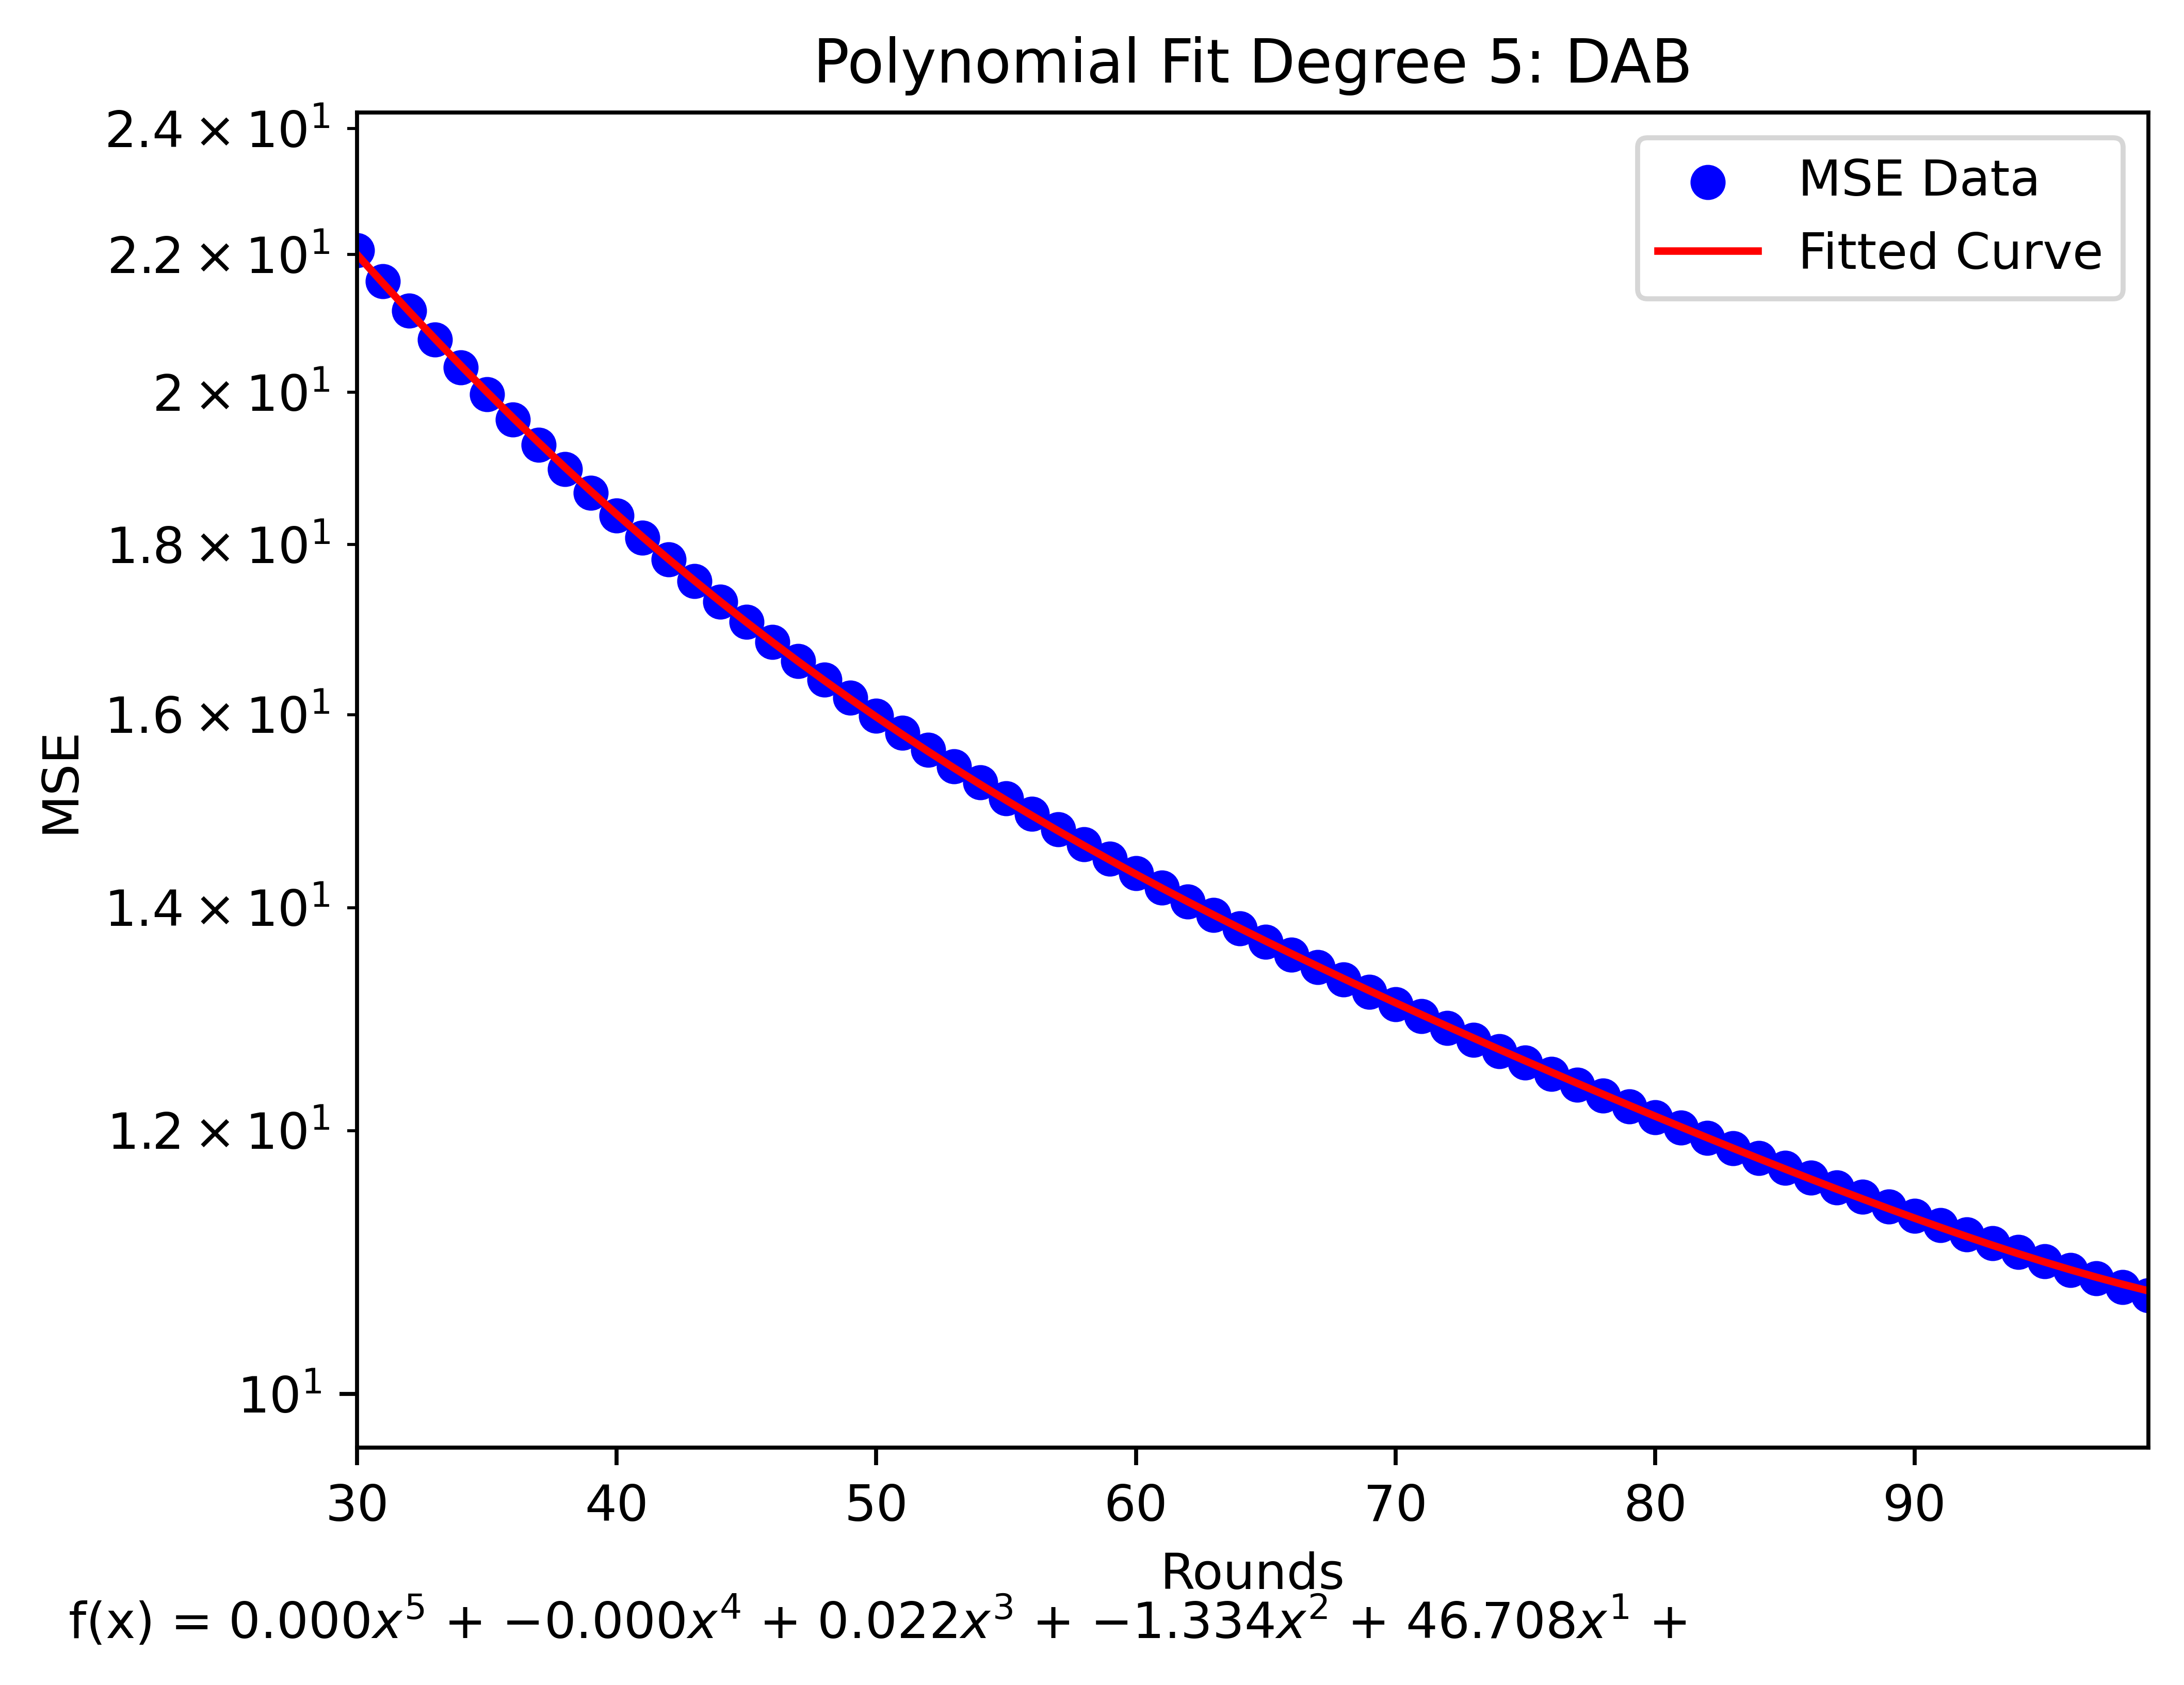
\includegraphics{figures/Simulation_outcomes/RingOfCliques/128x8/DAB/DAB_modelfitting_rounds_99_model_2.png}}
     \caption{$(128\times8)$-Ring of Cliques - polynomial regression fit: DAB}
     \label{fig:128x8dabRingOfCliquesModelFit}
\end{figure}
\begin{figure}[]
    \centering
    \scalebox{0.8}{\includegraphics{figures/Simulation_outcomes/RingOfCliques/128x8/PPS/PPS_modelfitting_rounds_99_model_2.png}}
    \caption{$(128\times8)$-Ring of Cliques - polynomial regression fit: PPS}
    \label{fig:128x8ppsRingOfCliquesModelFit}
\end{figure}

\begin{figure}[]
    \centering
    \scalebox{0.8}{\includegraphics{figures/Simulation_outcomes/RingOfCliques/128x8/ATPPS/ATPPS_modelfitting_rounds_99_model_2.png}}
    \caption{$(128\times8)$-Ring of Cliques - polynomial regression fit: ATPPS}
    \label{fig:128x8atppsRingOfCliquesModelFit}
\end{figure}

\begin{figure}
    \centering
    \scalebox{0.8}{\includegraphics{figures/Simulation_outcomes/RingOfCliques/128x8/DAB_vs_PPS_vs_ATPPS_slopesheatmap_100rounds.png}}
    \caption{$(128\times8)$-Ring of Cliques: heat map of slopes per region}
    \label{fig:128x8ringOfCliquesslopes}
\end{figure}

\subsection{8x128 Ring of Cliques}\label{subsec:8_128ROC}
Increasing the clique size and reducing the number of cliques favors the Push-Pull Sum based algorithms, which show a very steep decrease of error in the first 5 rounds of the simulation. The error is reduced by -200 on average in this region for each Push-Pull Sum based algorithm. The DAB data shows a more moderate decrease by -36 in this region. The error reduction reduces over the next regions, since the error of the network is already very low and the network is in a state of good balance showing a MSE in this region of around $\sim -30$ for the Push-Pull Sum based algorithms. After the first region the state of the network managed by the DAB is still very unbalanced and thus the balance potential is higher. This is shown by the slopes in the middle region. The Push-Pull Sum based algorithms reduce the error by $\sim -2$ while the DAB shows a still very high value of $\sim -30$. The reason behind this behavior is due to the impact of the clique sizes. The Push-Pull Sum based algorithms achieve good performances in reducing error in this scenario compared to the DAB which struggles in the context of dense graphs. The steep decrease and the low MSE values after rounds 5 and 10 stem from the fast error reduction in the cliques while still having to spread loads from clique to clique through the briding nodes. Compared to the experiment in the $(8 \times 128)$-Ring of Cliques in \ref{subsec:128_8ROC} the error after rounds 100 drop to lower values. After rounds 100 the DAB achieves a MSE value of 5.18 compared to 5.95 for the PPS and 4.56 for the ATPPS. especially in the last region (rounds 12 to 100) the DAB catches up to the PPS-based algorithms. However, the Push-Pull Sum based algorithms achieved a broadly balanaced state of the network after round 10 dropping the error to a MSE value of 7. In the following rounds the inter -clique error reduction follows. Here the PPS algorithm has difficulties, since the algorithms orders the nodes of the network to choose their transfer partner by random. The ATPPS has an advantage compared to the PPS here since it prioritizes the bridging nodes once its neighbors within the clique are already balanced. This elaborates why the PPS curve is mostly stagnating, while the ATPPS curve shows a downwards trend. The stagnating trend between rounds 20 to 100 is expressed by the linear mode fit in figure \ref{fig:8x128ppsRingOfCliquesModelFit}. The best-fit model follows the equation. $MSE_r=-0.0015x+6.05$. The PPS curve shows a complexer relation between the MSE reduction over the rounds, namely a polynomial of degree 2 following the equation $MSE_r=6.07\times 10^{-5}r^{2}-0.02r+6.39$ (figure \ref{fig:8x128ppsRingOfCliquesModelFit}). The DAB does not follow a single power relation ship in this region. Between the rounds 15 to 50 the error reduction can be expressed by a third degree polynomial $MSE_r=-3.33\times 10^{-3}r^{3}+0.63r^{2}-40.23r+872.75$ (figure \ref{fig:8x128atppsRingOfCliquesModelFit} a)) while in later rounds the power relation is a bit complexer, expressed by a fourth degree polynomial following the equation $MSE_r=2.96 \times 10^{-6}r^{4}-9.97\times 10^{-3}r^{3}+0.13r^{2}-7.16r+161.73$ (figure \ref{fig:8x128atppsRingOfCliquesModelFit} b)).

Snippets of the simulation outcomes after the 100th rounds of each load balancing algorithm verify that within the cliques the load is balanced, however the inter clique connection seems to be pending. Listing \ref{lst:exampleROCOutcomes} shows the simulation outcomes of two connected cliques balanced by the ATPPS in round 100. While the first clique converged to a value of $\sim 46.35$ the second clique averaged to $\sim 47.90$. The ground truth of the first clique is $45.89$ and the ground truth of the second clique is $48.13$. So the simulation outcomes and the ground truths align, however the averages do not align with the ground truth of the Ring of Cliques (which is $49.09$) itself. The PPS simulation outcomes show a similiar behavior.
\begin{figure}[!ht]
    \centering
        \subfloat[]{\includegraphics[width=0.49\linewidth]{figures/Simulation_outcomes/RingOfCliques/8x128/DAB_vs_PPS_RoC_r100_n1024_averaged_log.png}}
    \hfil
        \subfloat[]{\includegraphics[width=0.49\linewidth]{figures/Simulation_outcomes/RingOfCliques/8x128/DAB_vs_PPS_RoC_r100_n1024_averaged_loglog.png}}
    \caption{$(8\times128)$-Ring of Cliques: mean squared error per rounds (log-linear and log-log)}
        \label{fig:128x8RingOfCliquesLog_LogLog}
\end{figure}

\begin{figure}[!ht]
    \centering
        \subfloat[]{\includegraphics[width=0.49\linewidth]{figures/Simulation_outcomes/RingOfCliques/8x128/DAB/DAB_modelfitting_rounds_49_model_2.png}}
    \hfil
        \subfloat[]{\includegraphics[width=0.49\linewidth]{figures/Simulation_outcomes/RingOfCliques/8x128/DAB/DAB_modelfitting_rounds_99_model_2.png}}
    \caption{$(8\times128)$-Ring of Cliques - polynomial regression fit: rounds 20-50 and 55-100}
        \label{fig:8x128dabRingOfCliquesModelFit}
\end{figure}
\begin{figure}[]
    \centering
    \scalebox{0.8}{\includegraphics{figures/Simulation_outcomes/RingOfCliques/8x128/PPS/PPS_modelfitting_rounds_99_model_0.png}}
    \caption{$(8\times128)$-Ring of Cliques - polynomial regression fit: PPS}
    \label{fig:8x128ppsRingOfCliquesModelFit}
\end{figure}

\begin{figure}[]
    \centering
    \scalebox{0.8}{\includegraphics{figures/Simulation_outcomes/RingOfCliques/8x128/ATPPS/ATPPS_modelfitting_rounds_99_model_2.png}}
    \caption{$(8\times128)$-Ring of Cliques - polynomial regression fit: ATPPS}
    \label{fig:8x128atppsRingOfCliquesModelFit}
\end{figure}

\begin{figure}
    \centering
    \scalebox{0.8}{\includegraphics{figures/Simulation_outcomes/RingOfCliques/8x128/DAB_vs_PPS_vs_ATPPS_slopesheatmap_100rounds.png}}
    \caption{$(8\times128)$-Ring of Cliques: heat map of slopes per region}
    \label{fig:128x8ringOfCliquesslopes}
\end{figure}

\begin{lstlisting}[caption=Snippet of simulation outcomes ATPPS: Experiment 2, captionpos=b, label=lst:exampleROCOutcomes]
# First Clique starts here
ID 0	 sum 23.703116631927735	 weight 0.5112902995975737	 Average 46.359410007551446
ID 1	 sum 39.52476483621201	 weight 0.852801600538612	 Average 46.34696371494727
ID 2	 sum 8.793798989811481	 weight 0.18958634077240344	 Average 46.38413798158778
...
ID 125	 sum 94.3005473042508	 weight 2.0354736681273184	 Average 46.32855181615266
ID 126	 sum 145.10578299145917	 weight 3.1321941681390815	 Average 46.32719914604474
ID 127	 sum 149.43516229432458	 weight 3.222997634840688	 Average 46.365272092950555
# First Cliques ends here

# Second Clique starts here
ID 128	 sum 198.97437468622982	 weight 4.149869252421544	 Average 47.947143050380134
ID 129	 sum 168.24642313171216	 weight 3.5107838866374186	 Average 47.92275131832632
ID 130	 sum 35.6266112221637	 weight 0.7449330697151406	 Average 47.82525124812511
...
ID 253	 sum 63.87360335784297	 weight 1.3317373880292274	 Average 47.962611797185005
ID 254	 sum 15.173810743452982	 weight 0.31637895519911763	 Average 47.96087253623784
ID 255	 sum 19.982619800226413	 weight 0.4175626540105257	 Average 47.85538076334456
# Second Cliques ends here
\end{lstlisting}
    \chapter{Conclusion}\label{chap:conclusion}
The Adaptive Threshold Push-Pull Sum algorithm shows to be a compromise solution between the Push-Pull Sum and Single-Proposal Deal-Agreement-Based algorithms. The simulation results show that the Adaptive Threshold Push-Pull Sum algorithm performs well in dense graphs as well as in regular low-degree graphs. Especially for the Complete Graph $K_{1024}$, Ring of Cliques $ROC_{32,32}$ and $ROC_{8,128}$, as well as for Lollipop $L_{512,512}$ and $L_{896,128}$ topologies, the ATPPS algorithm proved to be the best solution, as the algorithm achieved the lowest MSE values after 100 rounds of simulation. The Adaptive Threshold Push-Pull Sum achieved good overall results. In cases where the PPS failed to show good balancing abilities, like in the $ROC_{32,32}$, the Adaptive Threshold Push-Pull Sum proved to be very efficient, achieving results close to the Deal-Agreement-Based algorithm. In cases where the Push-Pull Sum algorithm achieved lower MSE within 100 rounds, the difference to the Adaptive Threshold Push-Pull Sum algorithm was not significant as seen for the Star graph $S_{1024}$, the Lollipop graph $L_{128,896}$, as well as the Torus Grid $T_{32,32}$. However, when the Adaptive Threshold Push-Pull Sum outperforms the traditional Push-Pull Sum algorithm, the MSE discrepancies are more pronounced, like in the case of Ring of Cliques $ROC_{32,32}$ and $ROC_{128,8}$. Here, the Adaptive Threshold Push-Pull Sum algorithm manages to distribute loads efficiently by adapting to the network state. When the load differences within the cliques were no longer significant enough, clique-to-clique communication via the bridging nodes was favored. The Adaptive Threshold Push-Pull Sum algorithm also achieves the sharpest downward trend for $K_{1024}$ until the curve finally stagnates (due to the precision of doubles in Java). No improvement of the load balancing behavior was observed for the Ring $R_{1024}$ structure. The reason for this is that each node has exactly 2 neighbors, and thus only one neighbor is selected as $\lceil\log_{2}{(|neighborhood_{i}|)}\rceil$ evaluates to 1. The behavior of this algorithm is therefore very similar to the traditional Push-Pull Sum algorithm, without prioritizing any nodes. Also for the Star topology, the Adaptive Threshold Push-Pull Sum algorithm does not achieve any advantage over the traditional Push-Pull Sum algorithm, as the leaf nodes all communicate with the central node. The condition with significant load transfers limits the number of requests to the central node compared to the traditional Push-Pull Sum algorithm. The result: the Push-Pull Sum achieves a balanced state of the network earlier. Compared to the Push-Pull Sum algorithms, the Single-Proposal Deal-Agreement-Based algorithm has problems with dense graphs, such as the Complete graph, Lollipop graph with a large clique size, and Ring of Cliques with a large clique size. The MSE differences for dense graphs after 100 rounds of computation are extremely large between the Single-Proposal Deal-Agreement-Based algorithm and the Push-Pull Sum-based algorithms. For low-degree topologies such as the Ring graph and the Torus Grid graph the MSE differences are not as significant, especially between the best-performing Single-Proposal Deal-Agreement-Based algorithm and the Adaptive Threshold Push-Pull Sum algorithm. The simulation results depend mainly on the sensitivity factor $k$. A large $k$ ensures a more sensitive selection of neighbors, while a smaller $k$ allows a coarser selection of neighbors.
    \chapter{Outlook}\label{chap:outlook}
The proposed load balancing algorithm can be used in many different scenarios, like in cloud environments where many different servers are connected to a network, many with different hardware specifications. The method of randomized neighbour selection and the push and pull mechanisms allow an even distribution of loads throughout the network. The adaptive threshold condition only allows load transfers with a high impact on the balance of the network. The weight value can, for instance, represent the server capacities, i.e. given the hardware of a server, how capable it is of balancing the loads relative to the other partners in the network.

It is important to note that the performance of the algorithm was only tested in specific static topologies. Future research can also inspect dynamic networks. Furthermore, the performance was only tested with the metric of mean squared error and the trend of MSE decay was analysed with model fitting. However, further research is planned to compare the amount of messages sent to achieve low MSE values after r rounds. This would provide an insight into how efficient the load balancing mechanisms of the individual algorithms are.
    \chapter{Acknowledgments}

First and foremost, I would like to thank...
\begin{itemize}
\item{Saptadi Nugroho for his guidance and support throughout this thesis.}
\item{Prof. Dr. Christian Schindelhauer for giving me the opportunity to conduct this research at the chair of Computer Networks and Telematics. His critical questions and advice challenged me to refine my ideas and improved my work further.}
\item{my family for their support, patience, and encouragement throughout this journey. Their belief in me has been a constant source of motivation.}
\end{itemize}
    \chapter{Appendix}\label{chap:appendix}
\section{Model Fitting}\label{sec:modelfitting}
The model fitting was performed using the \textit{SciPy} and \textit{NumPy} libraries in Python. For fitting data to an exponential model, \textit{SciPy} provides the \textbf{curve\_fit} method. This method uses the Levenberg-Marquardt method to solve non-linear least squares problems \cite{SciPyCurveFit}. The linear regression was performed using the \textbf{linregress} method from \textit{scipy.stats}, which calculates a linear least squares regression for two sets of data points for x and y \cite{SciPyLinRegress}. For fitting the MSE data to a polynomial model of equation \ref{eq:polyfit}, \textit{NumPy}'s \textbf{polyfit} method was used.

\subsection{Levenberg-Marquardt Method}\label{subsec:lmMethod}
The Levenberg-Marquardt method is a hybrid of the Gauss-Newton method and the Levenberg method (Trust-Region approach). Starting from an initial guess for the parameters, the Levenberg-Marquardt method uses the Jacobian matrix to estimate how changes in parameters affect the fitted function. Then a damped least squares step is applied, where if the parameters are far from optimal, the Levenberg-Marquardt method behaves like the gradient descent, and if the parameters are near optimal, the Levenberg-Marquardt method acts like the Gauss-Newton method. It minimizes the sum of the squared residuals:
\begin{align}
    f(x)=\frac{1}{2}\sum_{j=1}^{m}{r_{j}^{2}(x)=\frac{1}{2}||r||^{2}},
\end{align}
where $f(x)$ is the objective function that we are trying to minimize, $r_{j}(x)$ represents the residuals (which are the differences between the observed data and the model predictions), and $r(x)$ is the vector of residuals, where $r(x)=[r_{1}(x), r_{2}(x),...,r_{n}(x)]^T$. The Gauss-Newton method is modified by a damping coefficient $\lambda$ and is written as:
\begin{align}
    (J^{T}J+ \lambda I)p = J^{T}r(x),
\end{align}
where $J$ is the Jacobian matrix of $r(x)$ (the derivatives of the residuals), $I$ is the identity matrix, and $\lambda$ controls the step size. $J^{T}J$ is the approximation of the Hessian matrix. $p$ is the update step. This equation is solved by iteratively reducing $f(x)$ until the parameters converge.

If $\lambda$ is large, the equation behaves like the gradient descent:
\begin{align}
    \lambda I p= J^{T}r(x),
\end{align}
while a small $\lambda$ causes the equation to behave like the Gauss-Newton method:
\begin{align}
    J^{T}Jp=J^{T}r(x).
\end{align}
\cite{gavin2020levenberg} \cite{Levenberg-Marquardt} \cite{broxOptimierung}

\subsection{SciPy's linregress}\label{subsec:linreg}
SciPy's \textbf{linregress} method fits data to a simple linear model as depicted in equation \ref{eq:linreg}. It achieves this by solving the \textit{Ordinary Least Squares} regression, which minimizes the sum of squared residuals. It returns the slope and the intercept of the fitted line, as well as the \textit{R-value} (\textit{Pearson's R}), \textit{p-value}, standard error of the estimated slope, and the standard error of the estimated intercept.
\cite{SciPyLinRegress} \cite{Wooditch2021}

\subsection{NumPy's polyfit and polyval}\label{subsec:polyfit}
The \textit{numpy.polyfit} method fits a polynomial of a given degree to a set of data points using the least squares minimization method \cite{NumPyPolyfit}. First, the Vandermonde Matrix is constructed, if given a degree $d$ and a set of data points $(x_1, y_1), (x_2, y_2), \dots, (x_n, y_n)$ of the form:
\begin{align}
    V =
    \begin{bmatrix} 
        x_{1}^{d} & x_{1}^{d-1} & \dots & x_{1}^{1} & 1 \\
        x_{2}^{d} & x_{2}^{d-1} & \dots & x_{2}^{1} & 1 \\
        \vdots & \vdots & \ddots & \vdots & \vdots \\
        x_{n}^{d} & x_{n}^{d-1} & \dots & x_{n}^{1} & 1 \\ 
    \end{bmatrix}.
\end{align}
Each row represents one data point, and each column corresponds to a power of $x$. Following the construction of the Vandermonde matrix, the polynomial coefficients $c=[c_{d},c_{d-1},...,c_{0}]$ are computed by solving:
\begin{align}
    c=(V^{T}V)^{-1}V^{T}y.
\end{align}
This method solves the linear least squares problem and ensures that the sum of squared residuals is minimized:
\begin{align}
    \sum_{i=1}{(y_{i}-P(x_i))^{2}},
\end{align}
where $P(x_{i})$ is the polynomial function. \cite{NumPyPolyfit} \cite{Vandermonde} \cite{GATechLS}

Once the polynomial coefficients are computed, the polynomial is evaluated using numpy's \textbf{polyval} method. This method internally uses \textit{Horner's method} in order to reduce the number of multiplications \cite{NumPyPolyVal}. For the polynomial of the form:
\begin{align}
    P(x) = a_{n}x^{n}+a_{n-1}x^{n-1}+ \dots + a_{1}x+a_{0},
\end{align}
it outputs a polynomial of form:
\begin{align}
    P(x)=p_{0}x^{n}+p_{1}^{n-1}+\dots + p_{n}.
\end{align}
\cite{wolfram_horner}

\section{Overview of Simulation Outcomes}\label{sec:overviewSimOutcomes}
The simulation outcomes are presented in the tables \ref{table:overviewcompletegraph}, \ref{table:overviewstar}, \ref{table:overviewring}, \ref{table:overviewtorus}, \ref{table:overview_Lollipop512_512}, \ref{table:overview_L128_896}, \ref{table:overview_L896_128}, \ref{table:overview_ROC_32_32}, \ref{table:overview_ROC_128_8}, and \ref{table:overview_ROC_8_128}. The tables contain the equations for the fitted models, the slopes in all regions, and the MSE value after 100 rounds of execution of the algorithms.

\begin{sidewaystable}
  \centering
  \caption{Simulation Overview - Complete graph: Fitted Model, Slopes per Region, and Final MSE}
  \label{table:overviewcompletegraph}
  \begin{tabular}{ll l c c c c c}
      \toprule
      \multicolumn{2}{l}{\textbf{Topology}} & \textbf{Fitted Model} & \textbf{Slope (log-linear)} \\ 
      & & & \shortstack{Rounds \\ 1--10} & \shortstack{Rounds \\ 11--65} & \shortstack{Rounds \\ 66--100} & \shortstack{Rounds \\ 1--100} & \shortstack{$MSE_{100}$} \\
      \midrule
      \multirow{3}{*}{$K_{1024}$} 
      & DAB   & \shortstack{\textbf{Rounds 1--100:} \\ $MSE_r = 844.63 \cdot e^{-0.01r}$}   & $-2.6 \times 10^{-3}$  & $-2.7 \times 10^{-3}$  & $-3.0 \times 10^{-3}$  & $-2.8 \times 10^{-3}$   & 436.85 \\
      & PPS   & \shortstack{\textbf{Rounds 10--80:} \\ $MSE_r = 2530.41 \cdot e^{-0.9r}$} & -0.38   & -0.39 & -0.16  & -0.31  & $1.73\times10^{-28}$ \\
      & ATPPS & \shortstack{\textbf{Rounds 10--65:} \\ $MSE_r = 4309.94 \cdot e^{-1.06r}$}   & -0.43   & -0.46 & -0.02  & -8.4  & $5.63\times10^{-28}$ \\
      \bottomrule
  \end{tabular}
\end{sidewaystable}


\begin{sidewaystable}
    \centering
    \caption{Simulation overview - Star graph: fitted model, slopes per region, and final MSE}
    \label{table:overviewstar}
    \begin{tabular}{ll l c c c c c}
        \toprule
        \multicolumn{2}{l}{\textbf{Topology}} & \textbf{Fitted Model} & \textbf{Slope (log-linear)} \\ 
        & & & \shortstack{Rounds \\ 1--10} & \shortstack{Rounds \\ 11--45} & \shortstack{Rounds \\ 46--100} & \shortstack{Rounds \\ 1--100} & \shortstack{$MSE_{100}$} \\
        \midrule
        \multirow{3}{*}{$S_{1024}$} 
        & DAB   & \shortstack{\textbf{Rounds 1--100:} \\ $MSE_r = 840.42 \cdot e^{-0.01r}$} & $-2.3 \times 10^{-3}$ & $-2.3 \times 10^{-3}$ & $-2.5 \times 10^{-3}$ & $-2.4 \times 10^{-3}$ & 480.48 \\
        & PPS   & \shortstack{\textbf{Rounds 10--45:} \\ $MSE_r = 29794.60 \cdot e^{-1.39r}$} & -0.5  & -0.6 & $-4.8 \times 10^{-3}$ & -0.26 & $8.31 \times 10^{-25}$ \\
        & ATPPS & \shortstack{\textbf{Rounds 18--60:} \\ $MSE_r = 9329.40 \cdot e^{-1.05r}$} & -0.45  & -0.45 & -0.11 & -0.26 & $6.52 \times 10^{-24}$ \\
        \bottomrule
    \end{tabular}
  \end{sidewaystable}
  

\begin{sidewaystable}
    \centering
    \caption{Simulation overview - Ring graph: fitted model, slopes per region, and final MSE}
    \label{table:overviewring}
    \begin{tabular}{ll l c c c c c}
        \toprule
        \multicolumn{2}{l}{\textbf{Topology}} & \textbf{Fitted Model} & \textbf{Slope (log-log)} \\ 
        & & & \shortstack{Rounds \\ 1--10} & \shortstack{Rounds \\ 11--69} & \shortstack{Rounds \\ 70--100} & \shortstack{Rounds \\ 1--100} & \shortstack{$MSE_{100}$} \\
        \midrule
        \multirow{3}{*}{$R_{1024}$} 
        & DAB   & \shortstack{\textbf{Rounds 10--60:} \\ $MSE_r=1.72 \times 10^{-5}r^{4} - 2.30 \times 10^{-3}r^{3}$\\ 
        $ + 0.19r^{2} - 5.99r + 114.83$} & -1.1 & -0.51 & -0.5 & -0.78  & 22.41 \\
        & PPS   & \shortstack{\textbf{Rounds 10--60:} \\ $MSE_r= 2.99 \times 10^{-5}r^{4} - 0.5 \times 10^{-2}r^{3}$ \\ $+ 0.32r^{2} - 9.68r + 166.30$} & -0.93 & -0.55 & -0.52 & -0.74  & 27.68 \\
        & ATPPS & \shortstack{\textbf{Rounds 10--60:} \\ $MSE_r= 3.04 \times 10^{-5}r^{4} - 0.5 \times 10^{-2}r^{3}$ \\ $+ 0.32r^{2} - 9.64r + 161.86$} & -0.95 & -0.56 & -0.49 & -0.75  & 26.56 \\
        \bottomrule
    \end{tabular}
  \end{sidewaystable}
  

\begin{sidewaystable}
  \centering
  \caption{Simulation overview - Torus Grid: fitted model, slopes per region, and final MSE}
  \label{table:overviewtorus}
  \begin{tabular}{ll l c c c c c}
      \toprule
      \multicolumn{2}{l}{\textbf{Topology}} & \textbf{Fitted Model} & \textbf{Slope} \\ 
      & & & \shortstack{Rounds \\ 1--10} & \shortstack{Rounds \\ 10--39} & \shortstack{Rounds \\ 40--100} & \shortstack{Rounds \\ 1--100} & \shortstack{$MSE_{100}$} \\
      \midrule
      \multirow{3}{*}{$T_{32,32}$} 
      & DAB   & \shortstack{\textbf{Rounds 10--39:} \\ 
      $MSE_r = -1.35 \times 10^{-6}r^{5} + 1.89 \times 10^{-4}r^{4}$ \\ 
      $- 0.01r^{3} + 0.30r^{2} - 4.6r + 34.10$ \\ 
      \textbf{Rounds 40--100:} \\ 
      $MSE_r = -6.01 \times 10^{-6}r^{3} + 1.66 \times 10^{-3}r^{2}$ \\ 
      $- 0.16r + 6$} 
      & -2.1 & -1.2 & -2 & -1.7 & 436.85 \\
      
      & PPS   & \shortstack{\textbf{Rounds 10--39:} \\ 
      $MSE_r = -3.65 \times 10^{-6}r^{5} + 5.16 \times 10^{-4}r^{4}$ \\ 
      $- 0.03r^{3} + 0.83r^{2} - 12.52r + 88.16$ \\ 
      \textbf{Rounds 40--100:} \\ 
      $MSE_r = -1.15 \times 10^{-5}r^{3} + 3.205 \times 10^{-3}r^{2}$ \\ 
      $- 0.33r + 13.72$} 
      & -1.5 & -1.2 & -1.4 & -1.4 & $1.73 \times 10^{-28}$ \\

      & ATPPS & \shortstack{\textbf{Rounds 10--39:} \\ 
      $MSE_r = -5.54 \times 10^{-6}r^{5} + 7.65 \times 10^{-4}r^{4}$ \\ 
      $- 0.04r^{3} + 1.16r^{2} - 16.81r + 112.86$ \\ 
      \textbf{Rounds 40--100:} \\ 
      $MSE_r = -9.99 \times 10^{-6}r^{3} + 2.8034 \times 10^{-3}r^{2}$ \\ 
      $- 0.28r + 11.29$} 
      & -1.6 & -1.3 & -1.7 & -1.5 & $5.63 \times 10^{-28}$ \\
      \bottomrule
  \end{tabular}
\end{sidewaystable}


\begin{sidewaystable}
  \centering
  \caption{Simulation overview for $L_{512,512}$: fitted model, slopes per region, and final MSE}
  \label{table:overview_L512_512}
  \begin{tabular}{ll l c c c c c}
      \toprule
      \multicolumn{2}{l}{\textbf{Topology}} & \textbf{Fitted Model} & \textbf{Slope} \\ 
      & & & \shortstack{Rounds \\ 1--7} & \shortstack{Rounds \\ 8--50} & \shortstack{Rounds \\ 51--100} & \shortstack{Rounds \\ 1--100} & \shortstack{$MSE_{100}$} \\
      \midrule
      \multirow{3}{*}{$L_{512,512}$} 
      & DAB   & \makecell[l]{$MSE_r=-5.89\times10^{-5}r^{3}+0.03r^{2}$ \\ $-5.68r+459.42$} & -67 & -4.5 & -2.6 & -7.3 & 108.90 \\
      & PPS   & \makecell[l]{$MSE_r=8.44\times 10^{-7}r^{4}-2.52\times 10^{-4}r^{3}$ \\ $-0.03r^{2}-1.64r+56.68$} & -130 & -0.9 & -0.12 & -8.3 & 14.71 \\
      & ATPPS & \makecell[l]{$MSE_r=8.69 \times 10^{-7}r^{4}-2.56 \times 10^{-4}r^{3}$ \\ $+0.03r^{2}-1.62r+54.48$} & -130 & -0.87 & -0.12 & -8.3 & 13.82 \\
      \bottomrule
  \end{tabular}
\end{sidewaystable}

\begin{sidewaystable}
  \centering
  \caption{Simulation overview for $L_{128,896}$: fitted model, slopes per region, and final MSE}
  \label{table:overview_L128_896}
  \begin{tabular}{ll l c c c c c}
      \toprule
      \multicolumn{2}{l}{\textbf{Topology}} & \textbf{Fitted Model} & \textbf{Slope} \\ 
      & & & \shortstack{Rounds \\ 1--7} & \shortstack{Rounds \\ 8--50} & \shortstack{Rounds \\ 51--100} & \shortstack{Rounds \\ 1--100} & \shortstack{$MSE_{100}$} \\
      \midrule
      \multirow{3}{*}{$L_{128,896}$} 
      & DAB   & \makecell[l]{$MSE_r=3.46\times 10^{-6}r^{4}-1.12\times 10^{-3}r^{3}$ \\ $+0.14r^{2}-7.69r+190.78$} & -110 & -2.8 & -0.25 & -8.2 & 17.47 \\
      & PPS   & \makecell[l]{$MSE_r=-3.72\times 10^{-8}r^{5}+1.31\times 10^{-5}r^{4}$ \\ $-1.85\times 10^{-3}r^{3}+0.13r^{2}-4.96r+84.91$} & -120 & -1.5 & $-7.6 \times 10^{-2}$ & -8.4 & 3.31 \\
      & ATPPS & \makecell[l]{$MSE_r=1.59\times 10^{-6}r^{4}-4.74\times 10^{-4}r^{3}$ \\ $+0.054r^{2}-2.94r+70.59$} & -120 & -1.6 & -0.13 & -8.4 & 3.41 \\
      \bottomrule
  \end{tabular}
\end{sidewaystable}

\begin{sidewaystable}
  \centering
  \caption{Simulation overview for $L_{128,896}$: fitted model, slopes per region, and final MSE}
  \label{table:overview_L128_896}
  \begin{tabular}{ll l c c c c c}
      \toprule
      \multicolumn{2}{l}{\textbf{Topology}} & \textbf{Fitted Model} & \textbf{Slope} \\ 
      & & & \shortstack{Rounds \\ 1--7} & \shortstack{Rounds \\ 8--50} & \shortstack{Rounds \\ 51--100} & \shortstack{Rounds \\ 1--100} & \shortstack{$MSE_{100}$} \\
      \midrule
      \multirow{3}{*}{$L_{128,896}$} 
      & DAB   & \makecell[l]{$MSE_r=3.46\times 10^{-6}r^{4}-1.12\times 10^{-3}r^{3}$ \\ $+0.14r^{2}-7.69r+190.78$} & -110 & -2.8 & -0.25 & -8.2 & 17.47 \\
      & PPS   & \makecell[l]{$MSE_r=-3.72\times 10^{-8}r^{5}+1.31\times 10^{-5}r^{4}$ \\ $-1.85\times 10^{-3}r^{3}+0.13r^{2}-4.96r+84.91$} & -120 & -1.5 & $-7.6 \times 10^{-2}$ & -8.4 & 3.31 \\
      & ATPPS & \makecell[l]{$MSE_r=1.59\times 10^{-6}r^{4}-4.74\times 10^{-4}r^{3}$ \\ $+0.054r^{2}-2.94r+70.59$} & -120 & -1.6 & -0.13 & -8.4 & 3.41 \\
      \bottomrule
  \end{tabular}
\end{sidewaystable}



\begin{sidewaystable}
  \centering
  \caption{Simulation overview - $ROC_{32,32}$: fitted model, slopes per region, and final MSE}
  \label{table:overview_ROC_32_32}
  \begin{tabular}{ll l c c c c c}
      \toprule
      \multicolumn{2}{l}{\textbf{Topology}} & \textbf{Fitted Model} & \textbf{Slope (log-log)} \\ 
      & & & \shortstack{Rounds \\ 1--5} & \shortstack{Rounds \\ 6--10} & \shortstack{Rounds \\ 11--100} & \shortstack{Rounds \\ 1--100} & \shortstack{$MSE_{100}$} \\
      \midrule
      \multirow{3}{*}{$ROC_{32,32}$} 
      & DAB   & \makecell[l]{$MSE_r=-5.89\times10^{-5}r^{3}+0.03r^{2}$ \\ $-5.68r+459.42$} & -0.51 & -2.1 & -1.1 & -1.1 & 6.55 \\
      & PPS   & \makecell[l]{$MSE_r=8.44\times 10^{-7}r^{4}-2.52\times 10^{-4}r^{3}$ \\ $-0.03r^{2}-1.64r+56.68$} & -1.8 & -0.61 & -0.09 & -0.81 & 19.80 \\
      & ATPPS & \makecell[l]{$MSE_r=8.69 \times 10^{-7}r^{4}-2.56 \times 10^{-4}r^{3}$ \\ $+0.03r^{2}-1.62r+54.48$} & -1.8 & -0.49 & -0.47 & -1 & 8.42 \\
      \bottomrule
  \end{tabular}
\end{sidewaystable}

\begin{sidewaystable}
  \centering
  \caption{Simulation overview for $ROC_{128,8}$: fitted model, slopes per region, and final MSE}
  \label{table:overview_ROC_128_8}
  \begin{tabular}{ll l c c c c c}
      \toprule
      \multicolumn{2}{l}{\textbf{Topology}} & \textbf{Fitted Model} & \textbf{Slope (log-log)} \\ 
      & & & \shortstack{Rounds \\ 1--5} & \shortstack{Rounds \\ 6--11} & \shortstack{Rounds \\ 12--100} & \shortstack{Rounds \\ 1--100} & \shortstack{$MSE_{100}$} \\
      \midrule
      \multirow{3}{*}{$ROC_{128,8}$} 
      & DAB   & \makecell[l]{$MSE_r=5.45\times 10 ^{-7}r^{4}-1.7\times 10^{-4}r^{3}$ \\ $+0.02r^{2}-1.33r+46.71$} & -1.4 & -0.75 & -0.66 & -0.95 & 10.64 \\
      & PPS   & \makecell[l]{$MSE_r=1.04\times 10 ^{-6}r^{4}-3.41\times 10^{-4}r^{3}$ \\ $+0.04r^{2}-2.73r+97.58$} & -1.3 & -0.36 & -0.55 & -0.79 & 22.33 \\
      & ATPPS & \makecell[l]{$MSE_r=9.54\times 10^{-7}r^{4}-2.93\times 10^{-4}r^{3}$ \\ $+0.03r^{2}-2.05r+67.02$} & -1.3 & -0.49 & -0.7 & -0.89 & 13.68 \\
      \bottomrule
  \end{tabular}
\end{sidewaystable}

\begin{sidewaystable}
  \centering
  \caption{Simulation overview - $ROC_{8,128}$: fitted model, slopes per region, and final MSE}
  \label{table:overview_ROC_8_128}
  \begin{tabular}{ll l c c c c c}
      \toprule
      \multicolumn{2}{l}{\textbf{Topology}} & \textbf{Fitted Model} & \textbf{Slope (log-log)} \\ 
      & & & \shortstack{Rounds \\ 1--5} & \shortstack{Rounds \\ 6--11} & \shortstack{Rounds \\ 12--100} & \shortstack{Rounds \\ 1--100} & \shortstack{$MSE_{100}$} \\
      \midrule
      \multirow{3}{*}{$ROC_{8,128}$} 
      & DAB   & \makecell[l]{$MSE_r=-3.33\times 10^{-3}r^{3}+0.63r^{2}$ \\ $-40.23r+872.75$ \\ \textbf{Rounds 60-100:} \\ $MSE_r=2.96 \times 10^{-6}r^{4}-9.97\times 10^{-3}r^{3}$ \\ $+0.13r^{2}-7.16r+161.73$} & -0.12 & -0.41 & -2.1 & -1.1 & 5.18 \\
      & PPS   & \makecell[l]{$MSE_r=6.07\times 10^{-5}r^{2}-0.02r+6.39$} & -2 & -1.9 & -0.01 & -1.1 & 5.95 \\
      & ATPPS & \makecell[l]{$MSE_r=-0.0015x+6.05$} & -2.1 & -1.6 & -0.13 & -1.1 & 4.56 \\
      \bottomrule
  \end{tabular}
\end{sidewaystable}


\section{Struggles of the Single-Proposal Deal-Agreement-Based Algorithm with Dense Graphs}\label{sec:struggleDAB}
Figure \ref{fig:specialcompletegraphDemo} illustrates a Complete graph with six nodes. The red node represents the minimally loaded node in the network that carries the load $L_{min}$. Using the Single-Proposal Deal-Agreement-Based algorithm, all blue nodes propose a load transfer to the red node. Since the red node now has five potential transfer options, it evaluates these options and accepts the option with maximal effect. This behavior also occurs with Complete graphs with a larger network size. In a graph where each node is interconnected, the balancing potential is usually high, as there are many options per node. However, in this stubborn deterministic way, this load balancing algorithm decreases the error only in very small steps.

A similar problem arises in the Star graph, as shown in figure \ref{fig:specialstargraphDemo}. All nodes have the central node as a neighbor. Now all leaves propose a load transfer to the central node, only now with the difference that the central node is not necessarily the minimally loaded node in the network (i.e., it does not carry $L_{min}$). The minimally loaded node in the example of figure \ref{fig:specialstargraphDemo} is a leaf node. The central node now receives a maximum of 4 proposals (i.e., exactly when the central node holds the second smallest load in the network) and accepts exactly one. If the central node is the maximally loaded node (i.e., the node that carries $L_{max}$), then there will be no proposals from the leaf nodes. Only the central node proposes the minimally loaded node, and that is the only load transfer.

In both scenarios, the number of load transfers is heavily limited.
\begin{figure}[]
    \centering
    \begin{tikzpicture}
    \foreach \i in {1,...,6} {
        \ifnum\i=1
            \node[draw, fill=red, circle, minimum size=20pt] (v\i) at ({360/6 * (\i-1)}:3) {};
        \else
            \node[draw, fill=blue, circle, minimum size=20pt] (v\i) at ({360/6 * (\i-1)}:3) {};
        \fi
    }
    
    \foreach \i in {1,...,6} {
        \foreach \j in {1,...,6} {
            \ifnum\i<\j
                \ifnum\i=1
                    \draw[->, line width=0.5mm, >=latex] (v\j) -- (v\i);
                \else
                    \draw[line width=0.2mm] (v\i) -- (v\j);
                \fi
            \fi
        }
    }
\end{tikzpicture}
    \caption{Complete graph: network size 6}
    \label{fig:specialcompletegraphDemo}
\end{figure}
\begin{figure}[]
    \centering
    \begin{tikzpicture}
    \node[draw, fill=blue, circle, minimum size=20pt] (center) at (0, 0) {}; % Central node in blue
    
    \foreach \i in {1,...,5} {
        \ifnum\i=1
            \node[draw, fill=red, circle, minimum size=20pt] (n\i) at ({360/5 * (\i-1)}:3) {}; % First outer node in red
        \else
            \node[draw, fill=blue, circle, minimum size=20pt] (n\i) at ({360/5 * (\i-1)}:3) {}; % Other outer nodes in blue
        \fi
        \draw[->, line width=0.5mm, >=latex] (n\i) -- (center);
    }
\end{tikzpicture}
    \caption{Star graph: network size 6}
    \label{fig:specialstargraphDemo}
\end{figure}
    
    % If you want a list of your ToDos at the end of the document
    % don't forget to remove before submission!
    % % place it somewhere in the document
\chapter*{ToDo Counters}
\newcounter{ct}%
To Dos: \arabic{todos}; \hspace{1em}%
\setcounter{ct}{0}%
\whiledo {\value{ct} < \value{todos}}%
{%
	\stepcounter {ct}%
    \ref{todo \thect}%
	\ifnum\value{ct} = \value{todos}{}\else{, }\fi
}

Parts to extend: \arabic{extends}; \hspace{1em}%
\setcounter{ct}{0}%
\whiledo {\value{ct} < \value{extends}}%
{%
	\stepcounter {ct}%
	\ref{extend \thect}%
	\ifnum\value{ct} = \value{extends}{}\else{, }\fi
}

Draft parts: \arabic{drafts}; \hspace{1em}%
\setcounter{ct}{0}%
\whiledo {\value{ct} < \value{drafts}}%
{%
	\stepcounter {ct}%
	\ref{draft \thect}%
	\ifnum\value{ct} = \value{drafts}{}\else{, }\fi
}


    \bibliographystyle{ieeetr}
    \bibliography{bib/main}
    % bibliography is not in the table of contents per default, add it manually
    % enable the \renewcommand for german header
    % \renewcommand{\bibname}{Literaturverzeichnis}
    \addcontentsline{toc}{chapter}{Bibliography}
    \newpage
    \thispagestyle{empty}
    \mbox{}


\end{document}
